% generated by GAPDoc2LaTeX from XML source (Frank Luebeck)
\documentclass[a4paper,11pt]{report}
\usepackage{geometry}
\usepackage{tikz}
\usetikzlibrary{positioning}

\usepackage{a4wide}
\sloppy
\pagestyle{myheadings}
\usepackage{amssymb}
\usepackage[latin1]{inputenc}
\usepackage{makeidx}
\makeindex
\usepackage{color}
\definecolor{FireBrick}{rgb}{0.5812,0.0074,0.0083}
\definecolor{RoyalBlue}{rgb}{0.0236,0.0894,0.6179}
\definecolor{RoyalGreen}{rgb}{0.0236,0.6179,0.0894}
\definecolor{RoyalRed}{rgb}{0.6179,0.0236,0.0894}
\definecolor{LightBlue}{rgb}{0.8544,0.9511,1.0000}
\definecolor{Black}{rgb}{0.0,0.0,0.0}

\definecolor{linkColor}{rgb}{0.0,0.0,0.554}
\definecolor{citeColor}{rgb}{0.0,0.0,0.554}
\definecolor{fileColor}{rgb}{0.0,0.0,0.554}
\definecolor{urlColor}{rgb}{0.0,0.0,0.554}
\definecolor{promptColor}{rgb}{0.0,0.0,0.589}
\definecolor{brkpromptColor}{rgb}{0.589,0.0,0.0}
\definecolor{gapinputColor}{rgb}{0.589,0.0,0.0}
\definecolor{gapoutputColor}{rgb}{0.0,0.0,0.0}

%%  for a long time these were red and blue by default,
%%  now black, but keep variables to overwrite
\definecolor{FuncColor}{rgb}{0.0,0.0,0.0}
%% strange name because of pdflatex bug:
\definecolor{Chapter }{rgb}{0.0,0.0,0.0}
\definecolor{DarkOlive}{rgb}{0.1047,0.2412,0.0064}


\usepackage{fancyvrb}

\usepackage{mathptmx,helvet}
\usepackage[T1]{fontenc}
\usepackage{textcomp}


\usepackage[
            pdftex=true,
            bookmarks=true,        
            a4paper=true,
            pdftitle={Written with GAPDoc},
            pdfcreator={LaTeX with hyperref package / GAPDoc},
            colorlinks=true,
            backref=page,
            breaklinks=true,
            linkcolor=linkColor,
            citecolor=citeColor,
            filecolor=fileColor,
            urlcolor=urlColor,
            pdfpagemode={UseNone}, 
           ]{hyperref}

\newcommand{\maintitlesize}{\fontsize{50}{55}\selectfont}

% write page numbers to a .pnr log file for online help
\newwrite\pagenrlog
\immediate\openout\pagenrlog =\jobname.pnr
\immediate\write\pagenrlog{PAGENRS := [}
\newcommand{\logpage}[1]{\protect\write\pagenrlog{#1, \thepage,}}
%% were never documented, give conflicts with some additional packages

\newcommand{\GAP}{\textsf{GAP}}

%% nicer description environments, allows long labels
\usepackage{enumitem}
\setdescription{style=nextline}

%% depth of toc
\setcounter{tocdepth}{1}





%% command for ColorPrompt style examples
\newcommand{\gapprompt}[1]{\color{promptColor}{\bfseries #1}}
\newcommand{\gapbrkprompt}[1]{\color{brkpromptColor}{\bfseries #1}}
\newcommand{\gapinput}[1]{\color{gapinputColor}{#1}}


\begin{document}

\logpage{[ 0, 0, 0 ]}
\begin{titlepage}
\mbox{}\vfill

\begin{center}{\maintitlesize \textbf{\textsf{YAGS}\mbox{}}}\\
\vfill

\hypersetup{pdftitle=\textsf{YAGS}}
\markright{\scriptsize \mbox{}\hfill \textsf{YAGS} \hfill\mbox{}}
{\Huge \textbf{Yet Another Graph System\mbox{}}}\\
\vfill

{\Huge Version 0.0.1\mbox{}}\\[1cm]
{15 August 2016\mbox{}}\\[1cm]
\mbox{}\\[2cm]
{\Large \textbf{R. MacKinney-Romero  \mbox{}}}\\
{\Large \textbf{M.A. Piza{\~n}a   \mbox{}}}\\
{\Large \textbf{ R. Villarroel-Flores   \mbox{}}}\\
\hypersetup{pdfauthor=R. MacKinney-Romero  ; M.A. Piza{\~n}a   ;  R. Villarroel-Flores   }
\mbox{}\\[2cm]
\begin{minipage}{12cm}\noindent
 {\centering \scalebox{0.8}{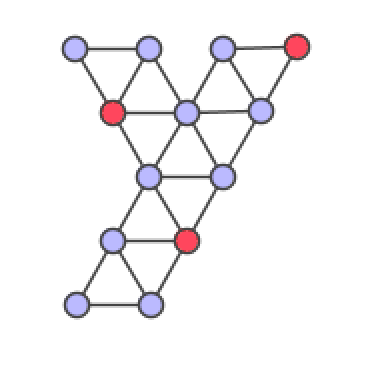
\includegraphics{yagslogo.png}}\par}  \end{minipage}

\end{center}\vfill

\mbox{}\\
{\mbox{}\\
\small \noindent \textbf{R. MacKinney-Romero  }  Email: \href{mailto://rene@xanum.uam.mx} {\texttt{rene@xanum.uam.mx}}}\\
{\mbox{}\\
\small \noindent \textbf{M.A. Piza{\~n}a   }  Email: \href{mailto://mpizana@gmail.com} {\texttt{mpizana@gmail.com}}\\
  Homepage: \href{http://xamanek.izt.uam.mx/map/} {\texttt{http://xamanek.izt.uam.mx/map/}}}\\
{\mbox{}\\
\small \noindent \textbf{ R. Villarroel-Flores   }  Email: \href{mailto://rafaelv@uaeh.edu.mx} {\texttt{rafaelv@uaeh.edu.mx}}\\
  Homepage: \href{http://rvf0068.github.io} {\texttt{http://rvf0068.github.io}}}\\
\end{titlepage}

\newpage\setcounter{page}{2}
{\small 
\section*{Copyright}
\logpage{[ 0, 0, 2 ]}
 

\textsf{YAGS} - Yet Another Graph System\\
 Copyright {\copyright} 2016 R. MacKinney-Romero, M.A. Piza{\~n}a and R.
Villarroel-Flores. 

This program is free software: you can redistribute it and/or modify it under
the terms of the GNU General Public License as published by the Free Software
Foundation, either version 3 of the License, or (at your option) any later
version. 

This program is distributed in the hope that it will be useful, but WITHOUT
ANY WARRANTY; without even the implied warranty of MERCHANTABILITY or FITNESS
FOR A PARTICULAR PURPOSE. See the GNU General Public License for more details. 

For details, see the file GPL in the installation directory of \textsf{YAGS} typically under \texttt{GAP-DIR/pkg/yags/GPL} or see \href{http://www.gnu.org/licenses/gpl-3.0.html} {\texttt{http://www.gnu.org/licenses/gpl-3.0.html}}. 

\textsc{Contact information:}\\
 M.A. Piza{\~n}a \\
 \href{mailto://yags@xamanek.izt.uam.mx} {\texttt{yags@xamanek.izt.uam.mx}}\\
 \href{mailto://mpizana@gmail.com} {\texttt{mpizana@gmail.com}}\\
  Departamento de Ingenier{\a'\i}a El{\a'e}ctrica\\
 Universidad Aut{\a'o}noma Metropolitana\\
 Av. San Rafael Atlixco 186.\\
 Col. Vicentina, Del. Iztapalapa\\
 Ciudad de M{\a'e}xico 09340 MEXICO.  \mbox{}}\\[1cm]
{\small 
\section*{Acknowledgements}
\logpage{[ 0, 0, 1 ]}
Partially supported by SEP-CONACyT, grant 183210. \\
\\
 We are also grateful for the support of our Universities:\\
 Universidad Aut{\a'o}noma Metropolitana and Universidad Aut{\a'o}noma del
Estado de Hidalgo. \mbox{}}\\[1cm]
\newpage

\def\contentsname{Contents\logpage{[ 0, 0, 3 ]}}

\tableofcontents
\newpage

 
\chapter{\textcolor{Chapter }{Preface}}\label{preface}
\logpage{[ 1, 0, 0 ]}
\hyperdef{L}{X874E1D45845007FE}{}
{
   
\section{\textcolor{Chapter }{Welcome to \textsf{YAGS}}}\label{welcometoyags}
\logpage{[ 1, 1, 0 ]}
\hyperdef{L}{X84CD2E0285ABBBC6}{}
{
  

\textsf{YAGS} - \emph{Yet Another Graph System} is a \textsf{GAP} package for dealing with graphs, in the sense of Graph Theory (not bar graphs,
pie charts nor graphs of functions). Our graphs are then, ordered pairs $G=(V,E)$, where $V$ is a finite set of vertices and $E$ is a finite set of edges which are (ordered or unordered) pairs of vertices. 

\textsf{YAGS} was initiated by M.A. Piza{\~n}a in May 2003, and soon incorporated the work
of R. MacKinney-Romero and R. Villarroel-Flores. It sprang from our need of
computing graphs and graph parameters within our research on graph theory and
clique graphs. Consequently, \textsf{YAGS} is well suited for these purposes. 

\textsf{YAGS} is a \textsf{GAP} package and hence its code is interpreted and not compiled (although some
compilation possibilities exist in \textsf{GAP}). Therefore, from the very beginning, it was clear that speed is not our main
goal. Instead, we wanted a very functional, full-featured system; a system
adequate for rapid prototyping of algorithms; and a quick, easy-to-use, way
for testing the rapidly changing working conjectures that are typical of the
research process. 

Over the years, \textsf{YAGS} grew to its present size of more than 200 methods and more than 10 thousands
lines of code. We considered that all this code and effort could (and should)
be useful for other people and then we decided to engage in the task of tying
up loose ends and writing this manual. 

We would like to mention that we started using \textsf{GRAPE}, and we are grateful to its author, Leonard H. Soicher, for the very useful
system that we used for several years. But at some point we needed some
Object-Oriented features that were not easy to implement in \textsf{GRAPE} and our own subsystem had to follow its own way. If the reader has a profound
need for having groups acting on her/his graphs, then \textsf{GRAPE} may be the best choice. On the other hand, \textsf{YAGS} offers a much wider set of functions (Appendix \ref{allalpha}); a graph-drawing subsystem (\texttt{Draw} (\ref{Draw})); many methods for dealing with graph homomorphism (Chapter \ref{morphismsofgraphs}); an Object-Oriented approach that simplifies the task of working with
several different graph categories (Chapter \ref{graphcategories}); and a generic backtracking subsystem useful to solve many combinatorial
problems easily (Chapter \ref{backtracking}). }

 
\section{\textcolor{Chapter }{Citing \textsf{YAGS}}}\label{citingyags}
\logpage{[ 1, 2, 0 ]}
\hyperdef{L}{X792C907981C4DFE4}{}
{
  

If you publish a result and you used \textsf{YAGS} during your research, please cite us as you would normally do with a research
paper:\\
\\
 R. MacKinney-Romero, M.A. Piza{\~n}a and R. Villarroel-Flores.\\
 \emph{YAGS - Yet Another Graph System, Version 0.0.1} (2016)\\
 \href{http://xamanek.izt.uam.mx/yags/} {\texttt{http://xamanek.izt.uam.mx/yags/}} 
\begin{verbatim}  
  @manual{YAGS,
    author = {R. MacKinney-Romero and M.A. Piza{\~n}a and R. Villarroel-Flores},
    title = {YAGS - Yet Another Graph System, Version 0.0.1},
    year = {2016},
    note = {http://xamanek.izt.uam.mx/yags/},
  }
\end{verbatim}
 

Several other citation formats can be obtained from the file \texttt{YAGS-DIR/CITATION} or by typing \texttt{Cite("yags");} at the \textsf{GAP} prompt. }

 
\section{\textcolor{Chapter }{Authors}}\label{authors}
\logpage{[ 1, 3, 0 ]}
\hyperdef{L}{X7B88101D7EE7EB10}{}
{
  

The authors of \textsf{YAGS} in the chronological order of their first contribution are as follows:\\
\\
 M.A. Piza{\~n}a\\
 Departamento de Ingenier{\a'\i}a El{\a'e}ctrica\\
 Universidad Aut{\a'o}noma Metropolitana\\
 \href{mailto://mpizana@gmail.com} {\texttt{mpizana@gmail.com}}\\
\\
 R. MacKinney-Romero\\
 Departamento de Ingenier{\a'\i}a El{\a'e}ctrica\\
 Universidad Aut{\a'o}noma Metropolitana\\
 \href{mailto://rene@xanum.uam.mx} {\texttt{rene@xanum.uam.mx}}\\
\\
 R. Villarroel-Flores\\
 Centro de Investigaci{\a'o}n en Matem{\a'a}ticas\\
 Universidad Aut{\a'o}noma del Estado de Hidalgo\\
 \href{mailto://rafaelv@uaeh.edu.mx} {\texttt{rafaelv@uaeh.edu.mx}} }

 
\section{\textcolor{Chapter }{More Information}}\label{moreinformation}
\logpage{[ 1, 4, 0 ]}
\hyperdef{L}{X80298E137C189819}{}
{
  

More information about \textsf{YAGS} can be found on its official web page and manual:\\
 \href{http://xamanek.izt.uam.mx/yags/} {\texttt{http://xamanek.izt.uam.mx/yags/}}\\
 \href{http://xamanek.izt.uam.mx/yags/doc/chap0.html} {\texttt{http://xamanek.izt.uam.mx/yags/doc/chap0.html}}\\
 \href{http://xamanek.izt.uam.mx/yags/manual.pdf} {\texttt{http://xamanek.izt.uam.mx/yags/manual.pdf}}\\
 

You can receive notifications about \textsf{YAGS} (i.e. new releases, bug fixes, etc.) by subscribing to its email distribution
list: \href{http://xamanek.izt.uam.mx/yagsnews/} {\texttt{http://xamanek.izt.uam.mx/yagsnews/}} 

If you are a developer, you may contribute to our project on our public
repository: \href{https://github.com/yags/yags/} {\texttt{https://github.com/yags/yags/}} 

Comments, support requests, bug reports and installation notifications are
welcome at \href{mailto://yags@xamanek.izt.uam.mx} {\texttt{yags@xamanek.izt.uam.mx}}. }

 }

 
\chapter{\textcolor{Chapter }{Getting Started}}\label{basics}
\logpage{[ 2, 0, 0 ]}
\hyperdef{L}{X7B1863E17896BCE1}{}
{
  
\section{\textcolor{Chapter }{What is \textsf{YAGS}?}}\label{whatisyags}
\logpage{[ 2, 1, 0 ]}
\hyperdef{L}{X83E7553782F04B65}{}
{
  

\textsf{YAGS} - \emph{Yet Another Graph System} is a \textsf{GAP} package for dealing with graphs, in the sense of Graph Theory (not bar graphs,
pie charts nor graphs of functions). Hence our graphs are ordered pairs $G=(V,E)$, where $V$ is a finite set of vertices and $E$ is a finite set of edges which are (ordered or unordered) pairs of vertices. 

\textsf{YAGS} was designed to be useful for research on graphs theory and clique graphs. It
is a very functional, full-featured system; a system adequate for rapid
prototyping of algorithms; and it is a quick, easy-to-use way, for testing the
rapidly changing working conjectures which are typical of the research
process. 

\textsf{YAGS} offers an ample set of functions (Appendix \ref{allalpha}); a graph-drawing subsystem (\texttt{Draw} (\ref{Draw})); many methods for dealing with graph homomorphism (Chapter \ref{morphismsofgraphs}); an Object-Oriented approach that simplifies the task of working with
several different graph categories (Chapter \ref{graphcategories}); and a generic backtracking subsystem useful to solve many combinatorial
problems easily (Chapter \ref{backtracking}). }

 
\section{\textcolor{Chapter }{Installing \textsf{YAGS} }}\label{installingyagsnow}
\logpage{[ 2, 2, 0 ]}
\hyperdef{L}{X7C143E16864EBAA6}{}
{
  

If you are fond of \texttt{git} and you already installed \textsf{GAP}, then you could clone our repository as usual (here we assume that \texttt{GAP-DIR} is your \textsf{GAP} installation directory): 

 
\begin{Verbatim}[commandchars=!@|,fontsize=\small,frame=single,label=Example]
  git clone http://github.com/yags/yags.git GAP-DIR/pkg/yags
\end{Verbatim}
 

Otherwise, you may follow these installation instructions: 
\begin{enumerate}
\item Install \textsf{GAP} following the instructions at \href{http://www.gap-system.org/} {\texttt{http://www.gap-system.org/}}. 
\item Obtain \textsf{YAGS} from its repository \href{https://github.com/yags/yags/archive/master.zip} {\texttt{https://github.com/yags/yags/archive/master.zip}}.
\item Unpack \textsf{YAGS}: the contents of the zip file should go under \texttt{GAP-DIR/pkg/yags/}. Here, we assume that \texttt{GAP-DIR} is your \textsf{GAP} installation directory.
\item Test \textsf{YAGS} by running \textsf{GAP}, loading \textsf{YAGS} and executing a few basic commands in a terminal: 

 
\begin{Verbatim}[commandchars=!@|,fontsize=\small,frame=single,label=Example]
  !gapprompt@>| !gapinput@gap|
     --- some GAP info here ---
  !gapprompt@gap>| !gapinput@RequirePackage("yags");|
  
  Loading  YAGS - Yet Another Graph System 0.0.1.
  Copyright (C) 2016 R. MacKinney-Romero, M.A. Pizana and R. Villarroel-Flores
  This is free software under GPLv3; for details type: ?yags:Copyright 
  
  true
  !gapprompt@gap>| !gapinput@CliqueNumber(Icosahedron);NumberOfCliques(Icosahedron);|
  3
  20
  !gapprompt@gap>| !gapinput@|
\end{Verbatim}

\item  (Optional) Make us happier by sending us a brief installation notification to \href{mailto://yags@xamanek.izt.uam.mx} {\texttt{yags@xamanek.izt.uam.mx}} and subscribing to \textsf{YAGS}'s distribution list: \href{http://xamanek.izt.uam.mx/yagsnews/} {\texttt{http://xamanek.izt.uam.mx/yagsnews/}} 
\end{enumerate}
 

Did it work? Congratulations! Otherwise, consider the following
troubleshooting issues: 


\begin{itemize}
\item \textsc{Is }\textsf{GAP}\textsc{ working?}\\
 Make sure it is. Follow carefully \textsf{GAP}'s installation and troubleshooting procedures. 
\item \textsc{Is the installation directory correct?}\\
 The \emph{\textsf{GAP}'s installation directory}, \texttt{GAP-DIR}, \index{GAP-DIR@\texttt{GAP-DIR}} \index{GAP's
      installation directory@\textsf{GAP}'s installation directory} is typically something like \texttt{/opt/gap4r8/} (in MS Windows it may look like \texttt{C:\texttt{\symbol{92}}gap4r8\texttt{\symbol{92}}}). If this is the case, the \emph{\textsf{YAGS}'s installation directory}, \texttt{YAGS-DIR}, is \index{YAGS-DIR@\texttt{YAGS-DIR}} \index{YAGS's
      installation directory@\textsf{YAGS}'s installation directory} \texttt{/opt/gap4r8/pkg/yags/} (in MS Windows, it would be \texttt{C:\texttt{\symbol{92}}gap4r8\texttt{\symbol{92}}pkg\texttt{\symbol{92}}yags\texttt{\symbol{92}}}). Then, the full path for \textsf{YAGS}'s info file \texttt{PackageInfo.g} should be \texttt{/opt/gap4r8/pkg/yags/PackageInfo.g} (or \texttt{C:\texttt{\symbol{92}}gap4r8\texttt{\symbol{92}}pkg\texttt{\symbol{92}}yags\texttt{\symbol{92}}PackageInfo.g}) 
\item \textsc{Are you using }\textsf{GRAPE}\textsc{?}\\
 \textsf{GRAPE} and \textsf{YAGS} are incompatible: they can not be loaded at the same time. If you had an
initialization file that loads \textsf{GRAPE} automatically, you should disable it in order to use \textsf{YAGS}. Alternatively, the command \texttt{gap -r} starts gap disabling any user-specific configuration files. 
\item \textsc{Unauthorized to access }\textsf{GAP}\textsc{'s directories?}\\
 The installation procedure above assumed that you have full access to your
computer (i.e. that you are the root of the system or that you are using your
PC or Mac). If this is not the case, you can also install \textsf{YAGS} under your user directory. For instance, if your user directory is \texttt{/home/joe/} then you can create a subdirectory \texttt{/home/joe/gaplocal/} and hence your \textsf{YAGS}'s installation directory will be \texttt{/home/joe/gaplocal/pkg/yags/}. Then you can start \textsf{GAP} using \texttt{gap -l ";/home/joe/gaplocal"} so that \textsf{GAP} knows where your \textsf{YAGS} is. 
\end{itemize}
 }

  
\section{\textcolor{Chapter }{A Gentle Tutorial}}\label{agentletutorial}
\logpage{[ 2, 3, 0 ]}
\hyperdef{L}{X875B75517E6E6576}{}
{
  

 This tutorial assumes that you already installed \textsf{GAP} and \textsf{YAGS}; and that you have some basic understanding of \textsf{GAP}: user interface, the read-eval-print loop, arithmetic operations, and lists.
It is strongly recommended that you have some \emph{working directory}, \texttt{WORKING-DIR}, \index{working directory} \index{WORKING-DIR} different from your \textsf{GAP}'s and \textsf{YAGS}'s installation directories. For instance, if your home directory is \texttt{/home/joe/} your working directory could be \texttt{/home/joe/Yags/}. Then you should open a terminal, move to your working directory, start \textsf{GAP} and then, load \textsf{YAGS}: 


\begin{Verbatim}[commandchars=!@|,fontsize=\small,frame=single,label=Example]
  /home/joe> cd Yags
  /home/joe/Yags> gap
     --- some GAP info here ---
  !gapprompt@gap>| !gapinput@RequirePackage("yags");|
  
  Loading  YAGS - Yet Another Graph System 0.0.1.
  Copyright (C) 2016 R. MacKinney-Romero, M.A. Pizana and R. Villarroel-Flores
  This is free software under GPLv3; for details type: ?yags:Copyright 
  
  true
  !gapprompt@gap>| !gapinput@|
\end{Verbatim}
 

The exact appearance of your system prompt (\texttt{/home/joe{\textgreater}} and \texttt{/home/joe/Yags/{\textgreater}} in the example) may be different depending on your system, but the commands '\texttt{cd Yags}' and '\texttt{gap}' are actually the same in all supported systems (assuming your working
directory exists and is named '\texttt{Yags}'). From there (starting with the command '\texttt{RequirePackage("yags");}') everything happens within \textsf{GAP} and hence it is system-independent. 

Now we want to define some graph. Say we have the list of edges of the desired
graph: 
\[ \{ \{ 1, 2 \}, \{ 2, 3 \}, \{ 3, 4 \}, \{ 4, 1 \}, \{ 1, 5 \}, \{ 5, 4 \} \} \]
 

We can put those edges in a list and then construct the graph: 

 
\begin{Verbatim}[commandchars=!@|,fontsize=\small,frame=single,label=Example]
  !gapprompt@gap>| !gapinput@list:=[[1,2],[2,3],[3,4],[4,1],[1,5],[5,4]];|
  [ [ 1, 2 ], [ 2, 3 ], [ 3, 4 ], [ 4, 1 ], [ 1, 5 ], [ 5, 4 ] ]
  !gapprompt@gap>| !gapinput@g:=GraphByEdges(list);                      |
  Graph( Category := SimpleGraphs, Order := 5, Size := 
  6, Adjacencies := [ [ 2, 4, 5 ], [ 1, 3 ], [ 2, 4 ], [ 1, 3, 5 ], 
    [ 1, 4 ] ] )
\end{Verbatim}
 

Note that \textsf{GAP} uses brackets ('\texttt{[}' and '\texttt{]}') instead of braces ('\texttt{\texttt{\symbol{123}}}' and '\texttt{\texttt{\symbol{125}}}') to represent sets and lists (actually, in \textsf{GAP} a set is simply an ordered list). Note also that in \textsf{GAP} '\texttt{list}' and '\texttt{List}' are two different things and you can not use the latter since it is a
reserved word of \textsf{GAP}. In general, it is better for you to use lowercase names for your variables,
to avoid name clashes, since all functions in \textsf{GAP} and \textsf{YAGS} start with an uppercase letter. 

The result in the previous example says that it is a graph, and a \emph{simple graph}. By default all graphs in \textsf{YAGS} are simple (no loops, no arrows, no parallel edges, only plain undirected
edges), in Chapter \ref{graphcategories} we explain how to work with other types of graphs, like digraphs, loopless
graphs, and graphs that may have loops (but no parallel edges are supported in \textsf{YAGS} at all). In this gentle tutorial all our graphs are simple. 

The result also says, that the just constructed graph \texttt{g} have \texttt{5} vertices and \texttt{6} edges. The reported list of adjacencies means that the vertex \texttt{1} is adjacent (connected by an edge) to \texttt{2}, \texttt{4} and \texttt{5}, that the vertex \texttt{2} is adjacent to \texttt{1} and \texttt{3} and so on. To be sure, we can draw our graph and check if it is the intended
graph: 


\begin{Verbatim}[commandchars=!@|,fontsize=\small,frame=single,label=Example]
  !gapprompt@gap>| !gapinput@Draw(g);|
\end{Verbatim}
 

A separate window appears with an editable drawing of the graph (but the graph
itself is not editable here). On that window, type: '\texttt{D}' (toggle dynamics on/off), '\texttt{L}' (toggle labels on/off) and '\texttt{F}' (fit graph into window) to obtain a nice drawing (the initial one is
random). The full list of keyboard commands for the \texttt{Draw} window is displayed when typing '\texttt{H}' (toggle help message). Besides these keyboard commands, you can use your
mouse in obvious ways to edit the drawing. 

To quit, type '\texttt{S}'. The drawing is stored within the graph \texttt{g} and remembered by \textsf{YAGS} in case you want to draw the graph again. 

If you are new to \textsf{GAP}, it may be worth mentioning that you need not remember or type all the full
names of every \textsf{YAGS} operation: \textsf{GAP} supports command completion. For instance, if you type \texttt{Path} and then hit the \texttt{{\textless}TAB{\textgreater}} key, \textsf{GAP} automatically completes the prefix to the unique command that completes it,
namely: \texttt{PathGraph}. If, on the other hand, the prefix has several possible completions, then \textsf{GAP} simply beeps, but a second \texttt{{\textless}TAB{\textgreater}} makes \textsf{GAP} respond with a list of possible completions, so you can then type some
additional keys and perhaps type \texttt{{\textless}TAB{\textgreater}} again, and so on. 


\begin{Verbatim}[commandchars=!@|,fontsize=\small,frame=single,label=Example]
  !gapprompt@gap>| !gapinput@GraphBy<TAB><TAB>|
      GraphByAdjMatrix
      GraphByAdjacencies
      GraphByCompleteCover
      GraphByEdges
      GraphByRelation
      GraphByWalks
  !gapprompt@gap>| !gapinput@GraphBy|
\end{Verbatim}
 

Also, the \texttt{{\textless}UP{\textgreater}} and \texttt{{\textless}DOWN{\textgreater}} keys are useful to bring back (and perhaps edit) some commands typed earlier
in your \textsf{GAP} session. As with any command in \textsf{GAP}/\textsf{YAGS}, in case of doubt, you can always access the online help by typing: 


\begin{Verbatim}[commandchars=!@|,fontsize=\small,frame=single,label=Example]
  !gapprompt@gap>| !gapinput@?yags:draw|
  Help: several entries match this topic - type ?2 to get match [2]
  
  [1] yags: Draw
  [2] yags: Drawing
  !gapprompt@gap>| !gapinput@?1|
    B.1-55 Draw
    
    > Draw( G ) --------------------------------------------- operation
    
    Takes a graph G and makes a drawing of it in a separate window. The
    user  can  then  view  and  modify the drawing and finally save the
    vertex coordinates of the drawing into the graph G.
    
    --- many more lines here ---
\end{Verbatim}
 

Here, '\texttt{?}' specifies that we want help; '\texttt{yags:}' specifies on which manual book we want to search (\textsf{YAGS}'s book in this case) and '\texttt{draw}' specifies the topic we would like to be informed about. As it is common,
there are more than one place with information on our topic, hence we choose
among the options with '\texttt{?1}' in the next command line. It is not necessary to specify the book, but then
you could receive many more options, in different books, about some specific
topic. 

Now that we know that our graph is the one we want, we can ask \textsf{YAGS} a lot of things about it: 

 
\begin{Verbatim}[commandchars=!@|,fontsize=\small,frame=single,label=Example]
  !gapprompt@gap>| !gapinput@Order(g); Size(g); Diameter(g); Girth(g);|
  5
  6
  2
  3
  !gapprompt@gap>| !gapinput@NumberOfCliques(g); CliqueNumber(g);                  |
  4
  3
  !gapprompt@gap>| !gapinput@Adjacencies(g);Adjacency(g,4);Adjacency(g,3);|
  [ [ 2, 4, 5 ], [ 1, 3 ], [ 2, 4 ], [ 1, 3, 5 ], [ 1, 4 ] ]
  [ 1, 3, 5 ]
  [ 2, 4 ]
  !gapprompt@gap>| !gapinput@VertexDegrees(g);VertexDegree(g,4);VertexDegree(g,3);|
  [ 3, 2, 2, 3, 2 ]
  3
  2
  !gapprompt@gap>| !gapinput@IsDiamondFree(g);IsCompleteGraph(g);IsLoopless(g);|
  true
  false
  true
  !gapprompt@gap>| !gapinput@Cliques(g);CompletesOfGivenOrder(g,3);|
  [ [ 1, 4, 5 ], [ 1, 2 ], [ 2, 3 ], [ 3, 4 ] ]
  [ [ 1, 4, 5 ] ]
  !gapprompt@gap>| !gapinput@CompletesOfGivenOrder(g,2);           |
  [ [ 1, 2 ], [ 1, 4 ], [ 1, 5 ], [ 2, 3 ], [ 3, 4 ], [ 4, 5 ] ]
\end{Verbatim}
 

Note that in \textsf{YAGS} a \emph{clique} is always \emph{maximal}. This is just a small sample. The full alphabetic list of \textsf{YAGS} operations can be found in Appendix \ref{allalpha}, and grouped by topic in Appendix \ref{alltopic}. There is also a one-page pdf file, \texttt{cheatsheet-yags.pdf}, which contains a very useful synopsis of many of the most common \textsf{YAGS} operations. See the next section (\ref{cheatsheet}) for details. 

What about \emph{modifying} our graphs\index{modifying graphs}? Well, all graphs in \textsf{YAGS} are always immutable, which means that, once created, we can never modify a
graph. But we can create new graphs which are variations of existing ones: 

 
\begin{Verbatim}[commandchars=!@|,fontsize=\small,frame=single,label=Example]
  !gapprompt@gap>| !gapinput@g;|
  Graph( Category := SimpleGraphs, Order := 5, Size := 
  6, Adjacencies := [ [ 2, 4, 5 ], [ 1, 3 ], [ 2, 4 ], [ 1, 3, 5 ], 
    [ 1, 4 ] ] )
  !gapprompt@gap>| !gapinput@h:=AddEdges(g,[[1,3],[2,4]]);;  |
  !gapprompt@gap>| !gapinput@g;|
  Graph( Category := SimpleGraphs, Order := 5, Size := 
  6, Adjacencies := [ [ 2, 4, 5 ], [ 1, 3 ], [ 2, 4 ], [ 1, 3, 5 ], 
    [ 1, 4 ] ] )
  !gapprompt@gap>| !gapinput@h;|
  Graph( Category := SimpleGraphs, Order := 5, Size := 
  8, Adjacencies := [ [ 2, 3, 4, 5 ], [ 1, 3, 4 ], [ 1, 2, 4 ], 
    [ 1, 2, 3, 5 ], [ 1, 4 ] ] )
\end{Verbatim}
 

Note that the graph \texttt{g} remains the same, but the graph \texttt{h} has two additional edges. This is done in this way, because in \textsf{YAGS} everything that is computed about a graph is stored within the graph, so that
we never need to compute something twice. This saves time when computing
attributes of graphs requiring CPU-intensive algorithms (like computing
cliques and clique graphs), but at the expense of having to make a copy of the
graph when we just want a small variation of it. 

 There are a lot of predefined graphs (the full list can be consulted in
Appendix \ref{tfamilies}): 

 
\begin{Verbatim}[commandchars=!@|,fontsize=\small,frame=single,label=Example]
  !gapprompt@gap>| !gapinput@PathGraph(5);CycleGraph(6);CompleteGraph(5); |
  Graph( Category := SimpleGraphs, Order := 5, Size := 
  4, Adjacencies := [ [ 2 ], [ 1, 3 ], [ 2, 4 ], [ 3, 5 ], [ 4 ] ] )
  Graph( Category := SimpleGraphs, Order := 6, Size := 
  6, Adjacencies := [ [ 2, 6 ], [ 1, 3 ], [ 2, 4 ], [ 3, 5 ], [ 4, 6 ], 
    [ 1, 5 ] ] )
  Graph( Category := SimpleGraphs, Order := 5, Size := 
  10, Adjacencies := [ [ 2, 3, 4, 5 ], [ 1, 3, 4, 5 ], [ 1, 2, 4, 5 ], 
    [ 1, 2, 3, 5 ], [ 1, 2, 3, 4 ] ] )
  !gapprompt@gap>| !gapinput@CompleteBipartiteGraph(3,3);TreeGraph([2,2,2]);|
  Graph( Category := SimpleGraphs, Order := 6, Size := 
  9, Adjacencies := [ [ 4, 5, 6 ], [ 4, 5, 6 ], [ 4, 5, 6 ], 
    [ 1, 2, 3 ], [ 1, 2, 3 ], [ 1, 2, 3 ] ] )
  Graph( Category := SimpleGraphs, Order := 15, Size := 
  14, Adjacencies := [ [ 2, 3 ], [ 1, 4, 5 ], [ 1, 6, 7 ], [ 2, 8, 9 ], 
    [ 2, 10, 11 ], [ 3, 12, 13 ], [ 3, 14, 15 ], [ 4 ], [ 4 ], [ 5 ], 
    [ 5 ], [ 6 ], [ 6 ], [ 7 ], [ 7 ] ] )
  !gapprompt@gap>| !gapinput@Octahedron;ParapluieGraph;|
  Graph( Category := SimpleGraphs, Order := 6, Size := 
  12, Adjacencies := [ [ 3, 4, 5, 6 ], [ 3, 4, 5, 6 ], [ 1, 2, 5, 6 ], 
    [ 1, 2, 5, 6 ], [ 1, 2, 3, 4 ], [ 1, 2, 3, 4 ] ] )
  Graph( Category := SimpleGraphs, Order := 7, Size := 
  9, Adjacencies := [ [ 2 ], [ 1, 3 ], [ 2, 4, 5, 6, 7 ], [ 3, 5 ], 
    [ 3, 4, 6 ], [ 3, 5, 7 ], [ 3, 6 ] ] )
\end{Verbatim}
 

We have found that \texttt{GraphByWalks} (\ref{GraphByWalks}) is one of the most useful and versatile ways of specifying graphs: 

 
\begin{Verbatim}[commandchars=!@|,fontsize=\small,frame=single,label=Example]
  !gapprompt@gap>| !gapinput@p5:=PathGraph(5);;c6:=CycleGraph(6);;w4:=WheelGraph(4);;  |
  !gapprompt@gap>| !gapinput@IsIsomorphicGraph(p5,GraphByWalks([1..5]));|
  true
  !gapprompt@gap>| !gapinput@IsIsomorphicGraph(c6,GraphByWalks([1,2,3,4,5,6,1]));|
  true
  !gapprompt@gap>| !gapinput@IsIsomorphicGraph(c6,GraphByWalks([1..6],[6,1]));   |
  true
  !gapprompt@gap>| !gapinput@IsIsomorphicGraph(w4,GraphByWalks([1,[2,3,4,5,2]]));|
  true
  !gapprompt@gap>| !gapinput@sd:=GraphByWalks([1,[2,3,4,5],6],[5,[6,7,8,1],2]);; |
  !gapprompt@gap>| !gapinput@IsIsomorphicGraph(SnubDisphenoid,sd);|
  true
\end{Verbatim}
 

\textsf{YAGS} knows about random graphs, so you can take some random graphs and study their
parameters. Furthermore, \texttt{GraphAttributeStatistics} (\ref{GraphAttributeStatistics}) can collect statistics on 100 random graphs at a time returning the collected
results of the specified graph parameter on these graphs. The following experiments show, for instance that the values of the minimum
degree parameter are much more spread than those of the clique number or those
of the diameter. 

 
\begin{Verbatim}[commandchars=!@|,fontsize=\small,frame=single,label=Example]
  !gapprompt@gap>| !gapinput@MinDeg:=function(G) return Minimum(VertexDegrees(G)); end;;|
  !gapprompt@gap>| !gapinput@g:=RandomGraph(30,1/2);; MinDeg(g); CliqueNumber(g); Diameter(g);|
  9
  6
  2
  !gapprompt@gap>| !gapinput@GraphAttributeStatistics(30,1/2,MinDeg);|
  [ [ 5, 1 ], [ 6, 2 ], [ 7, 6 ], [ 8, 22 ], [ 9, 30 ], [ 10, 30 ], 
    [ 11, 5 ], [ 12, 4 ] ]
  !gapprompt@gap>| !gapinput@GraphAttributeStatistics(30,1/2,CliqueNumber);|
  [ [ 5, 2 ], [ 6, 70 ], [ 7, 24 ], [ 8, 4 ] ]
  !gapprompt@gap>| !gapinput@GraphAttributeStatistics(30,1/2,Diameter);    |
  [ [ 2, 91 ], [ 3, 9 ] ]
\end{Verbatim}
 

Finally, it is worth mentioning that algorithms the may take too much time to
finish report their progress using the \texttt{InfoLevel} mechanism: Enabling and disabling progress reporting is done by changing the \texttt{InfoLevel} of \texttt{YAGSInfo.InfoClass} to the appropriate level. The default \texttt{InfoLevel} is 0. Some of \textsf{YAGS} algorithms report at \texttt{InfoLevel} 1, and others at \texttt{InfoLevel} 3. 

 
\begin{Verbatim}[commandchars=!@|,fontsize=\small,frame=single,label=Example]
  !gapprompt@gap>| !gapinput@SetInfoLevel(YAGSInfo.InfoClass,3);           |
  !gapprompt@gap>| !gapinput@FullMonoMorphisms(PathGraph(3),CycleGraph(3));|
  #I [  ]
  #I [ 1 ]
  #I [ 1, 2 ]
  #I [ 1, 3 ]
  #I [ 2 ]
  #I [ 2, 1 ]
  #I [ 2, 3 ]
  #I [ 3 ]
  #I [ 3, 1 ]
  #I [ 3, 2 ]
  [  ]
  !gapprompt@gap>| !gapinput@SetInfoLevel(YAGSInfo.InfoClass,0);           |
  !gapprompt@gap>| !gapinput@FullMonoMorphisms(PathGraph(3),CycleGraph(3));|
  [  ]
\end{Verbatim}
 

This way we can abort the calculation (by typing \texttt{Ctr-C}) in case we see that it will take eons to finish. See \texttt{YAGSInfo.InfoClass} (\ref{YAGSInfo.InfoClass}) for details. }

 
\section{\textcolor{Chapter }{Cheatsheet}}\label{cheatsheet}
\logpage{[ 2, 4, 0 ]}
\hyperdef{L}{X7AC1C7197E9E9112}{}
{
  

There is a very useful one-page pdf cheatsheet with \textsf{YAGS}'s most common functions. It can be consulted in your \textsf{YAGS} installation at \texttt{YAGS-DIR/doc/cheatsheet-yags.pdf} or on the web at \href{http://xamanek.izt.uam.mx/yags/cheatsheet-yags.pdf} {\texttt{http://xamanek.izt.uam.mx/yags/cheatsheet-yags.pdf}}. Also, the pdf version of this manual includes it in the next page.  \newpage\thispagestyle{empty}%
\newgeometry{left=0.1cm,top=0.87cm,bottom=0.1cm,right=0.1cm}%
\noindent\scalebox{1}{\rotatebox{90}{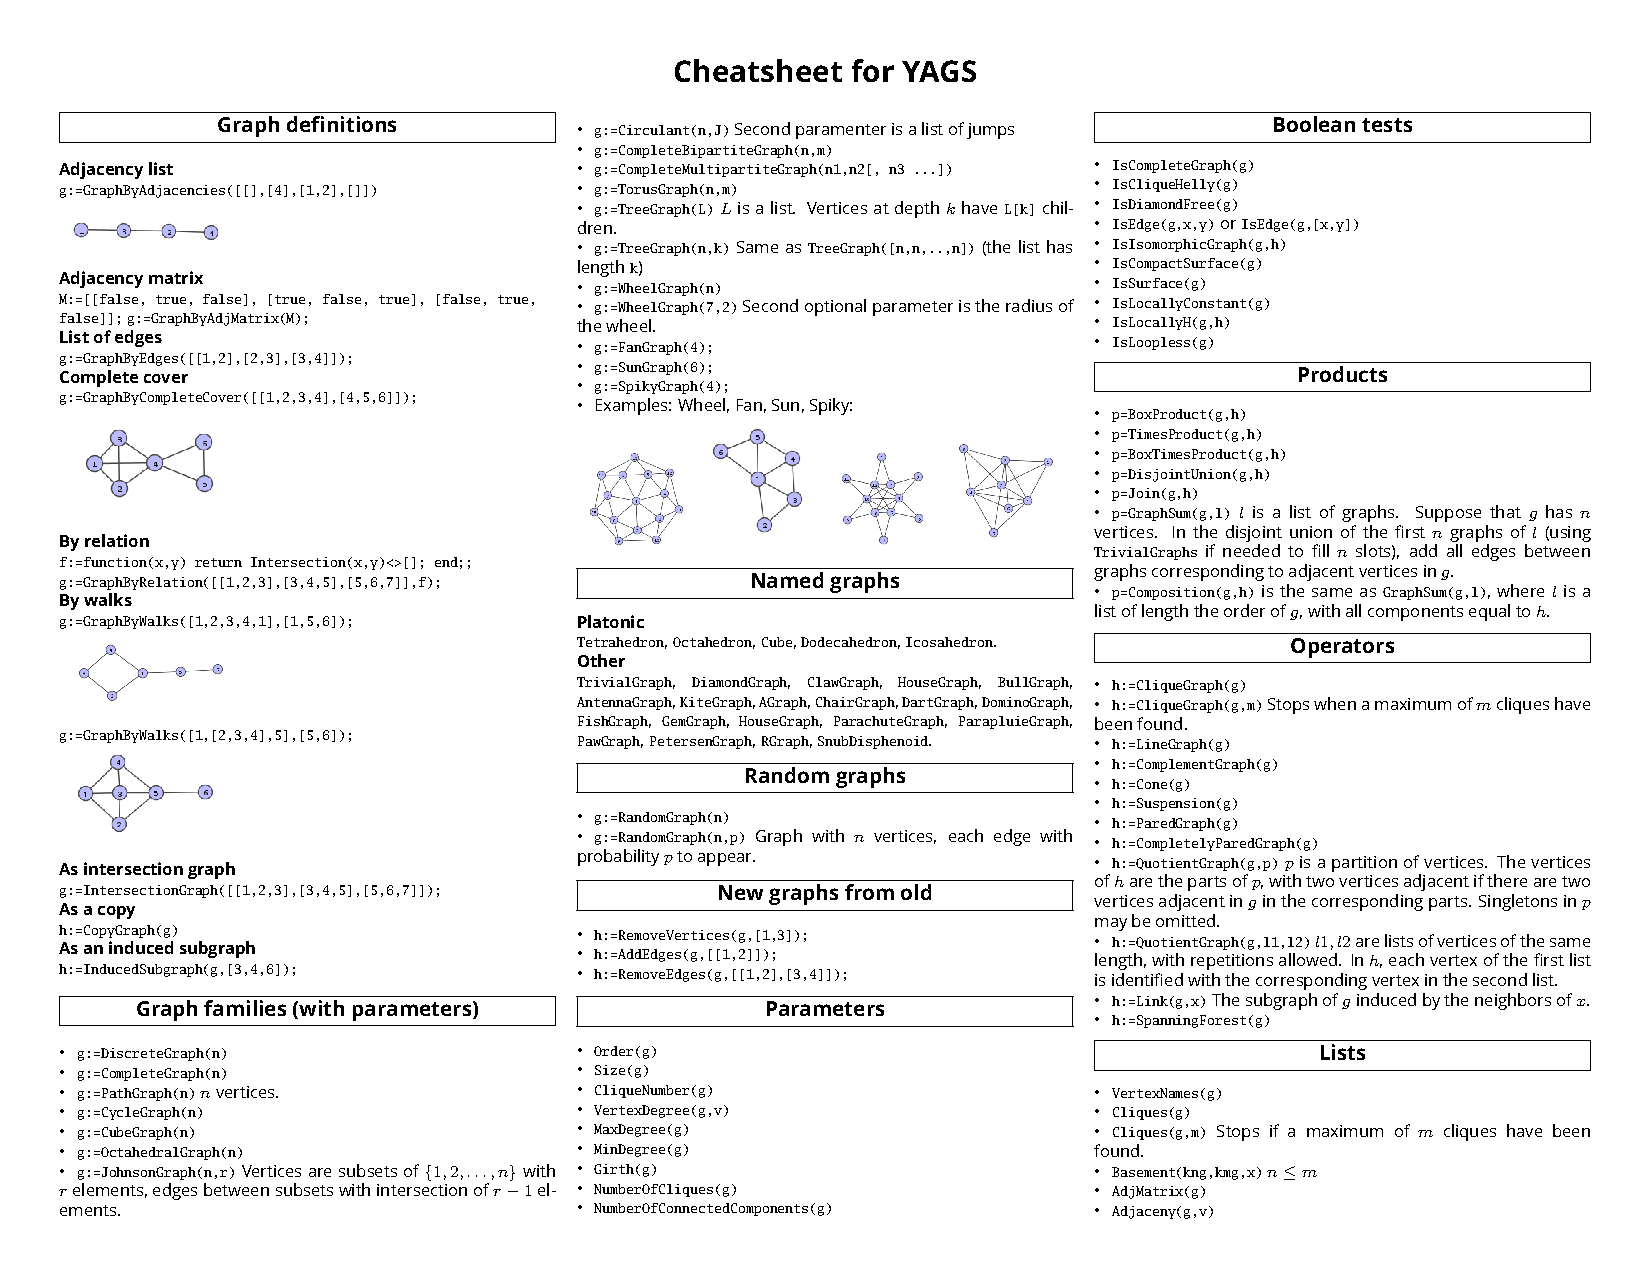
\includegraphics{cheatsheet-yags.pdf}}}%
\restoregeometry  }

 }

 \restoregeometry 
\chapter{\textcolor{Chapter }{Cliques and Clique Graphs}}\label{cliques}
\logpage{[ 3, 0, 0 ]}
\hyperdef{L}{X784B470D87297C9D}{}
{
  

A \emph{clique}\index{clique} is a maximal complete subgraph (other texts use \emph{maxclique} for this concept). It is common to identify induced subgraphs of a graph with
their vertex sets; accordingly, a clique in \textsf{YAGS} is actually a set of vertices of a graph such that any two vertices in the
clique are adjacent in the considered graph. 

The \emph{clique graph}\index{clique graph}, $K(G)$, of a graph $G$ is the intersection graph of all the cliques of $G$: Each clique of $G$ is a vertex of $K(G)$, two of them are adjacent in $K(G)$ if and only if they have a non-empty intersection. 

A number of \textsf{YAGS}'s features concerning cliques and clique graphs are described in this
chapter. 
\section{\textcolor{Chapter }{Cliques and Clique Number}}\label{cliquesandcliquenumber}
\logpage{[ 3, 1, 0 ]}
\hyperdef{L}{X786467B78756F151}{}
{
  

You can get the set of all the cliques of a graph by means of \texttt{Cliques} (\ref{Cliques}); if you want to know the completes of given order (maximal or not) you may
use \texttt{CompletesOfGivenOrder} (\ref{CompletesOfGivenOrder}) instead. 

 
\begin{Verbatim}[commandchars=!@|,fontsize=\small,frame=single,label=Example]
  !gapprompt@gap>| !gapinput@g:=SunGraph(4);;|
  !gapprompt@gap>| !gapinput@Cliques(g);|
  [ [ 2, 4, 6, 8 ], [ 2, 3, 4 ], [ 1, 2, 8 ], [ 4, 5, 6 ], [ 6, 7, 8 ] ]
  !gapprompt@gap>| !gapinput@CompletesOfGivenOrder(g,3);|
  [ [ 1, 2, 8 ], [ 2, 3, 4 ], [ 2, 4, 6 ], [ 2, 4, 8 ], [ 2, 6, 8 ], 
    [ 4, 5, 6 ], [ 4, 6, 8 ], [ 6, 7, 8 ] ]
  !gapprompt@gap>| !gapinput@CompletesOfGivenOrder(g,4);|
  [ [ 2, 4, 6, 8 ] ]
\end{Verbatim}
 

Note that \texttt{CompletesOfGivenOrder} uses a simple, straightforward backtracking algorithm, whereas \texttt{Cliques} uses the Bron-Kerbosch algorithm \cite{BK73}\index{Bron-Kerbosch algorithm} which in our experience is the best algorithm for finding all cliques of a
graph in practice. In particular, \texttt{Cliques} is much faster than \texttt{CompletesOfGivenOrder} (when comparable). 

\index{mutable graphs}\index{immutable graphs} In \textsf{YAGS} all graphs are \emph{immutable}, that is, once created, all graphs always remain exactly the same graph. If
you need to modify a graph, you actually construct a new graph by copying the
first graph and (for example) adding or deleting some edges (all of this in a
single atomic step) therefore creating a new immutable graph. All
graph-modifying operations in \textsf{YAGS} (e.g. \texttt{AddEdges}, \texttt{RemoveEdges}, etc.) work in this way. This is time-consuming if your work involves many
frequent graph editions. On the other hand, this design decision allows us to
meaningfully store all computed graph attributes within the graph itself:
Since the graph is not going to change ever, it will always have the same
order, size, clique number, etc. \textsf{YAGS} does exactly this with all graph attributes and properties. This means that no
attribute is ever computed twice for the same graph and in particular it has a
very clear effect on computing time: 
\begin{Verbatim}[commandchars=!@|,fontsize=\small,frame=single,label=Example]
  !gapprompt@gap>| !gapinput@g:=RandomGraph(200);;                  |
  !gapprompt@gap>| !gapinput@Cliques(g);;time;    |
  5784
  !gapprompt@gap>| !gapinput@Cliques(g);;time;    |
  0
\end{Verbatim}
 

The \emph{clique number}\index{clique number}, $\omega(G)$\index{omega@$\omega(G)$}, is the order of a maximum clique (all cliques are maximal, but they may be
of several different orders). On the other hand, the \emph{number of cliques}\index{cliques@!number
  of}\index{number of cliques}, is simply the cardinality of the set of all cliques. 

 
\begin{Verbatim}[commandchars=!@|,fontsize=\small,frame=single,label=Example]
  !gapprompt@gap>| !gapinput@g:=SunGraph(4);;|
  !gapprompt@gap>| !gapinput@CliqueNumber(g);|
  4
  !gapprompt@gap>| !gapinput@NumberOfCliques(g);|
  5
\end{Verbatim}
 

For random graphs with edge probability $p$ and taking $b:=1/p$, it is known \cite{Bol01} that the distribution of the clique number has a very concentrated peak around $2\log_{b}n-2\log_{b}\log_{b}n +2\log_{b}(\frac{e}{2})$: 

 
\begin{Verbatim}[commandchars=!@|,fontsize=\small,frame=single,label=Example]
  !gapprompt@gap>| !gapinput@GraphAttributeStatistics([10,20..70],1/2,CliqueNumber);|
  [ [ [ 3, 29 ], [ 4, 61 ], [ 5, 9 ], [ 6, 1 ] ], 
    [ [ 4, 5 ], [ 5, 64 ], [ 6, 31 ] ], 
    [ [ 5, 5 ], [ 6, 64 ], [ 7, 29 ], [ 8, 2 ] ], 
    [ [ 6, 20 ], [ 7, 72 ], [ 8, 8 ] ], 
    [ [ 7, 55 ], [ 8, 42 ], [ 9, 3 ] ], 
    [ [ 7, 17 ], [ 8, 75 ], [ 9, 7 ], [ 10, 1 ] ], 
    [ [ 8, 66 ], [ 9, 32 ], [ 10, 2 ] ] ]
  !gapprompt@gap>| !gapinput@List([10,20..70],n->2*Log2(Float(n))                        |
  !gapprompt@>| !gapinput@-2*Log2(Log2(Float(n))) + 2*Log2(FLOAT.E/2));             |
  [ 4.0652, 5.3059, 6.10955, 6.70535, 7.17974, 7.57437, 7.91252 ]
\end{Verbatim}
 Not so much the distribution of the number of cliques: 
\begin{Verbatim}[commandchars=!@|,fontsize=\small,frame=single,label=Example]
  !gapprompt@gap>| !gapinput@GraphAttributeStatistics([10,20..70],1/2,NumberOfCliques);|
  [ [ [ 7, 4 ], [ 8, 4 ], [ 9, 18 ], [ 10, 23 ], [ 11, 23 ], 
        [ 12, 13 ], [ 13, 8 ], [ 14, 5 ], [ 16, 1 ], [ 17, 1 ] ], 
    [ [ 36, 1 ], [ 40, 2 ], [ 41, 3 ], [ 42, 1 ], [ 43, 4 ], 
        [ 44, 4 ], [ 45, 2 ], [ 46, 4 ], [ 47, 1 ], [ 48, 5 ], 
        [ 49, 2 ], [ 50, 1 ], [ 51, 5 ], [ 52, 6 ], [ 53, 6 ], 
        [ 54, 5 ], [ 55, 6 ], [ 56, 4 ], [ 57, 5 ], [ 58, 7 ], 
        [ 59, 4 ], [ 60, 2 ], [ 61, 3 ], [ 62, 3 ], [ 63, 4 ], 
        [ 64, 3 ], [ 66, 3 ], [ 67, 1 ], [ 68, 1 ], [ 72, 1 ], 
        [ 77, 1 ] ], 
     [ [ 130, 1 ], [ 133, 1 ], [ 135, 1 ], [ 137, 1 ], [ 142, 1 ],
        
     --- many more lines here ---
  
        [ 4626, 1 ], [ 4629, 1 ] ] ]
\end{Verbatim}
 }

 
\section{\textcolor{Chapter }{Clique Graphs}}\label{cliquegraphs}
\logpage{[ 3, 2, 0 ]}
\hyperdef{L}{X7EC084CC84A85A76}{}
{
  

Whenever we have a graph $G$, we can compute its clique graph $K(G)$, which is the intersection graph of the cliques of $G$. Much work has been done on clique graphs \cite{Szw03}\cite{Pri95b}\cite{LPV14} and they have even been applied to Loop Quantum Gravity \cite{Req00a}\cite{Req00b}\cite{Req03}. It is know that deciding whether a given graph is a clique graph ($G\cong K(H)$ for some $H$) is NP-complete \cite{AFFG09}. 

Computing the clique graph of a graph is clearly an exponential time operation
in the worst case as the maximum number of cliques of a graph of order $n$ is $\alpha\times 3^{\frac{n-\alpha}{3}}= \Theta(3^{\frac{n}{3}})$ \cite{MM65} (here $\alpha$ it taken such that $\alpha \in \{2,3,4\}$ and $n\equiv \alpha$ mod 3). However, very often the number of cliques in a graph is much smaller; the
following experiment shows that the number of cliques of a graph on 50
vertices is likely between 700 and 1300 instead of the maximum possible which
is $2\times3^{16}=86093442$. 

 
\begin{Verbatim}[commandchars=!@|,fontsize=\small,frame=single,label=Example]
  !gapprompt@gap>| !gapinput@GraphAttributeStatistics(50,1/2,NumberOfCliques);|
  [ [ 756, 1 ], [ 762, 1 ], [ 770, 1 ], [ 795, 1 ], [ 826, 2 ], 
    [ 832, 1 ], [ 834, 1 ], [ 835, 1 ], [ 856, 1 ], [ 860, 1 ], 
    [ 861, 1 ], [ 867, 2 ], [ 870, 1 ], [ 871, 2 ], [ 872, 1 ], 
    [ 886, 1 ], [ 887, 1 ], [ 891, 1 ], [ 896, 1 ], [ 897, 2 ], 
    [ 898, 1 ], [ 905, 1 ], [ 911, 1 ], [ 916, 2 ], [ 920, 2 ], 
    [ 923, 2 ], [ 934, 1 ], [ 938, 1 ], [ 940, 1 ], [ 942, 1 ], 
    [ 943, 1 ], [ 944, 1 ], [ 949, 1 ], [ 953, 1 ], [ 963, 1 ], 
    [ 965, 1 ], [ 966, 1 ], [ 967, 2 ], [ 970, 1 ], [ 971, 1 ], 
    [ 972, 1 ], [ 973, 2 ], [ 975, 1 ], [ 978, 1 ], [ 985, 1 ], 
    [ 986, 1 ], [ 988, 1 ], [ 993, 1 ], [ 994, 2 ], [ 997, 1 ], 
    [ 998, 1 ], [ 999, 2 ], [ 1002, 1 ], [ 1008, 1 ], [ 1015, 1 ], 
    [ 1020, 2 ], [ 1022, 1 ], [ 1025, 1 ], [ 1026, 1 ], [ 1028, 1 ], 
    [ 1029, 1 ], [ 1034, 1 ], [ 1047, 1 ], [ 1049, 1 ], [ 1054, 1 ], 
    [ 1062, 1 ], [ 1067, 1 ], [ 1069, 1 ], [ 1071, 1 ], [ 1075, 1 ], 
    [ 1077, 1 ], [ 1087, 1 ], [ 1088, 1 ], [ 1097, 1 ], [ 1098, 1 ], 
    [ 1102, 1 ], [ 1135, 1 ], [ 1139, 1 ], [ 1154, 1 ], [ 1159, 2 ], 
    [ 1165, 1 ], [ 1187, 1 ], [ 1191, 1 ], [ 1192, 1 ], [ 1203, 1 ], 
    [ 1217, 1 ], [ 1236, 1 ] ]
  !gapprompt@gap>| !gapinput@2*3^16;|
  86093442
\end{Verbatim}
 

Therefore, we can often compute cliques and clique graphs \emph{in practice}, despite the worst case exponential time. Also, \texttt{CliqueGraph} is an attribute of graphs (as most operations in \textsf{YAGS}) and hence, the result is stored within the graph in order to prevent
unnecessary recalculation: 

 
\begin{Verbatim}[commandchars=!@|,fontsize=\small,frame=single,label=Example]
  !gapprompt@gap>| !gapinput@g:=RandomGraph(80);;     |
  !gapprompt@gap>| !gapinput@kg:=CliqueGraph(g);;time;|
  26499
  !gapprompt@gap>| !gapinput@kg2:=CliqueGraph(g);;time;|
  0
  !gapprompt@gap>| !gapinput@kg2=kg;|
  true
\end{Verbatim}
 

Note that the last line in the previous example is \emph{not} testing for isomorphism, it only tests whether both adjacency matrices are
equal. It remains possible, however, that the graph at hand is one of those
with a huge number of cliques. We can limit the maximum number of cliques to
be computed in \texttt{Cliques} and \texttt{CliqueGraph} using the optional extra parameter \mbox{\texttt{\mdseries\slshape maxNumCli}}: With this extra parameter, the computation is aborted when the number of
computed cliques reaches \mbox{\texttt{\mdseries\slshape maxNumCli}}. 

 
\begin{Verbatim}[commandchars=!@|,fontsize=\small,frame=single,label=Example]
  !gapprompt@gap>| !gapinput@g:=OctahedralGraph(3);; |
  !gapprompt@gap>| !gapinput@CliqueGraph(g,1000); |
  Graph( Category := SimpleGraphs, Order := 8, Size := 
  24, Adjacencies := [ [ 2, 3, 4, 5, 6, 7 ], [ 1, 3, 4, 5, 6, 8 ], 
    [ 1, 2, 4, 5, 7, 8 ], [ 1, 2, 3, 6, 7, 8 ], [ 1, 2, 3, 6, 7, 8 ], 
    [ 1, 2, 4, 5, 7, 8 ], [ 1, 3, 4, 5, 6, 8 ], [ 2, 3, 4, 5, 6, 7 ] ] )
  !gapprompt@gap>| !gapinput@g:=OctahedralGraph(30);; #this has 2^30=1073741824 cliques.|
  !gapprompt@gap>| !gapinput@CliqueGraph(g,1000);                            |
  fail
\end{Verbatim}
 

Alternatively we can use the \texttt{InfoLevel} mechanism (\ref{YAGSInfo.InfoClass}) to be informed about the progress of clique-related operations in \textsf{YAGS}. This way we can abort the calculation (by typing \texttt{Ctr-C}) in case we see that it will take eons to finish. 

In \textsf{YAGS} the vertices of a graph are always \texttt{[1, 2, ..., Order(G)]}, but often they also have some \emph{names}. This names depend on the way in which the graph is constructed and reflect
the origin of the graph. We can get the names of the vertices by using \texttt{VertexNames} (\ref{VertexNames}). In the case of clique graphs, the vertex names are the corresponding cliques
of the original graph. 

 
\begin{Verbatim}[commandchars=!@|,fontsize=\small,frame=single,label=Example]
  !gapprompt@gap>| !gapinput@g:=SunGraph(4);          |
  Graph( Category := SimpleGraphs, Order := 8, Size := 
  14, Adjacencies := [ [ 2, 8 ], [ 1, 3, 4, 6, 8 ], [ 2, 4 ], 
    [ 2, 3, 5, 6, 8 ], [ 4, 6 ], [ 2, 4, 5, 7, 8 ], [ 6, 8 ], 
    [ 1, 2, 4, 6, 7 ] ] )
  !gapprompt@gap>| !gapinput@kg:=CliqueGraph(g);|
  Graph( Category := SimpleGraphs, Order := 5, Size := 
  8, Adjacencies := [ [ 2, 3, 4, 5 ], [ 1, 3, 4 ], [ 1, 2, 5 ], 
    [ 1, 2, 5 ], [ 1, 3, 4 ] ] )
  !gapprompt@gap>| !gapinput@VertexNames(kg);|
  [ [ 2, 4, 6, 8 ], [ 2, 3, 4 ], [ 1, 2, 8 ], [ 4, 5, 6 ], [ 6, 7, 8 ] ]
  !gapprompt@gap>| !gapinput@Cliques(g);|
  [ [ 2, 4, 6, 8 ], [ 2, 3, 4 ], [ 1, 2, 8 ], [ 4, 5, 6 ], [ 6, 7, 8 ] ]
\end{Verbatim}
 

Hence, in the previous example, vertex 1 of \texttt{kg} is (the one corresponding to) the clique \texttt{[ 2, 4, 6, 8 ]} of \texttt{g}, and vertex 2 is \texttt{[ 2, 3, 4 ]} etc. }

 
\section{\textcolor{Chapter }{Basements and Iterated Clique Graphs}}\label{basements}
\logpage{[ 3, 3, 0 ]}
\hyperdef{L}{X85C4B82682FEED6C}{}
{
  

Iterated clique graphs\index{Iterated clique graphs} are obtained by applying the clique operator several times. As before, we may
wonder which vertices of $K^3(g)$ constitute the clique corresponding to some vertex of $K^4(g)$ and this can be settled using \texttt{VertexNames} as explained in Section \ref{cliquegraphs}. But what if we want to know which vertices of $g$ constitute some vertex of $K^4(g)$? This could be done using \texttt{VertexNames} at level $K^4(g)$ and then transforming each of the obtained vertices (in $K^3(g)$) using \texttt{VertexNames} of $K^3(g)$ and so on... but \textsf{YAGS} already has an operation that does exactly that. The \emph{basement}\index{basement} of a vertex $x$ of an iterated clique graph $K^n(g)$ with respect to some previous iterated clique graph $K^m(g)$ (with $m\leq n$) is, roughly speaking, the set of vertices of $K^m(g)$ that constitute the vertex $x$, that is, the set of vertices of $K^m(g)$ which are needed for $x$ to exist (see \texttt{Basement} (\ref{Basement}) for a formal definition). 

 
\begin{Verbatim}[commandchars=!@|,fontsize=\small,frame=single,label=Example]
  !gapprompt@gap>| !gapinput@K:=CliqueGraph;|
  <Attribute "CliqueGraph">
  !gapprompt@gap>| !gapinput@g:=Icosahedron;;Order(g); |
  12
  !gapprompt@gap>| !gapinput@kg:=K(g);;Order(kg);          |
  20
  !gapprompt@gap>| !gapinput@k2g:=K(kg);;Order(k2g);|
  32
  !gapprompt@gap>| !gapinput@k3g:=K(k2g);;Order(k3g);|
  92
  !gapprompt@gap>| !gapinput@k4g:=K(k3g);;Order(k4g);|
  472
  !gapprompt@gap>| !gapinput@VertexNames(kg)[1];VertexNames(kg)[3];  |
  [ 1, 2, 3 ]
  [ 1, 3, 4 ]
  !gapprompt@gap>| !gapinput@Basement(g,kg,1);Basement(g,kg,3);        |
  [ 1, 2, 3 ]
  [ 1, 3, 4 ]
  !gapprompt@gap>| !gapinput@VertexNames(k4g)[2];VertexNames(k4g)[9];|
  [ 1, 2, 55, 72, 73, 74, 80, 81, 82, 83, 84, 85, 88, 89, 90 ]
  [ 1, 2, 3, 4, 10, 16, 81, 82, 85, 87, 88, 89 ]
  !gapprompt@gap>| !gapinput@Basement(k3g,k4g,2);Basement(k3g,k4g,9);|
  [ 1, 2, 55, 72, 73, 74, 80, 81, 82, 83, 84, 85, 88, 89, 90 ]
  [ 1, 2, 3, 4, 10, 16, 81, 82, 85, 87, 88, 89 ]
  !gapprompt@gap>| !gapinput@Basement(k2g,k4g,9);|
  [ 1, 2, 3, 4, 5, 6, 7, 17, 19, 24, 25, 27, 28, 29, 30, 31 ]
  !gapprompt@gap>| !gapinput@Basement(kg,k4g,9); |
  [ 1, 2, 3, 4, 5, 7, 8, 11, 12, 13, 14, 15, 16, 17, 18, 19, 20 ]
  !gapprompt@gap>| !gapinput@Basement(g,k4g,9); |
  [ 1, 2, 3, 4, 5, 6, 7, 8, 9, 10, 11, 12 ]
\end{Verbatim}
 

Basements where introduced (with a different name) in \cite{BS95} and used again in \cite{Piz04}. They have been useful to study distances and diameters on iterated clique
graphs. They are also useful when dealing with stars and neckties. }

 
\section{\textcolor{Chapter }{Stars and Neckties}}\label{starsandneckties}
\logpage{[ 3, 4, 0 ]}
\hyperdef{L}{X8371E7537E137D0C}{}
{
  

Stars and neckties are useful in understanding the structure of iterated
clique graphs. 

Let $G$ be a graph and $x\in G$. Let us define $x^*:=\{q\in K(G) : x\in q\}$. We say that $x^*$ is the \emph{star} of $x$\index{star@!of a
  vertex}. Observe that $x^*$ is (induces) a complete subgraph of $K(G)$, and may or may not be a clique of $K(G)$ (i.e. a vertex of $K^2(G)$) depending on whether the star of $x$ is a \emph{maximal} complete subgraph or not. 

On the other hand, a vertex in $K^2(G)$ is of the form $Q:=\{q_1,q_2,\ldots,q_r\}$ where each $q_i$ is a clique of $G$ (i.e. a vertex of $K(G)$). We say that such \emph{clique of cliques}\index{clique of cliques} $Q$ is \emph{a star}\index{star} if there is some vertex $x\in G$ such that $x\in q_i$ for all $q_i\in Q$; equivalently $Q$ is a star if the total intersection of its cliques is non-empty (i.e. $\cap Q \neq \varnothing$). When $Q$ is not a star (i.e. when $\cap Q = \varnothing$), we say it is a \emph{necktie}\index{necktie}. It is easy to show that a clique of cliques $Q$ is a star if and only if its basement at $G$ is exactly the closed neighborhood of a vertex $N[x]$. 

Clearly, a star is also the star of some vertex and any star of a vertex which
is a clique of cliques is a star. On the other hand, if the star of a vertex $x^*$ is not a clique of cliques, it is surely contained in some clique of cliques $Q\in K^2(G)$. If for each vertex $x$ we pick such a fixed clique of cliques $*(x):=Q\in K^2(G)$ with $x^*\subseteq Q$, we get the star morphism $*:G\rightarrow K^2(G)$\index{star morphism}. 

A very remarkable feature of the second iterated clique graph $K^2(G)$ of $G$ is that the star morphism is often injective and even an isomorphism onto its
image. 

 
\begin{Verbatim}[commandchars=!@|,fontsize=\small,frame=single,label=Example]
  !gapprompt@gap>| !gapinput@g:=Icosahedron;;                                 |
  !gapprompt@gap>| !gapinput@kg:=K(g);;k2g:=K(kg);;|
  !gapprompt@gap>| !gapinput@ClosedNeighborhood:=function(g,x)|
  !gapprompt@>| !gapinput@return Union(Adjacency(g,x),[x]); end;       |
  function( g, x ) ... end
  !gapprompt@gap>| !gapinput@closNeighs:=List(Vertices(g),x->ClosedNeighborhood(g,x)); |
  [ [ 1 .. 6 ], [ 1, 2, 3, 6, 9, 10 ], [ 1, 2, 3, 4, 10, 11 ], 
    [ 1, 3, 4, 5, 7, 11 ], [ 1, 4, 5, 6, 7, 8 ], [ 1, 2, 5, 6, 8, 9 ], 
    [ 4, 5, 7, 8, 11, 12 ], [ 5, 6, 7, 8, 9, 12 ], 
    [ 2, 6, 8, 9, 10, 12 ], [ 2, 3, 9, 10, 11, 12 ], 
    [ 3, 4, 7, 10, 11, 12 ], [ 7 .. 12 ] ]
  !gapprompt@gap>| !gapinput@stars:=Filtered(Vertices(k2g),|
  !gapprompt@>| !gapinput@Q->Basement(g,k2g,Q) in closNeighs); |
  [ 1, 3, 5, 8, 10, 12, 15, 18, 21, 24, 27, 30 ]
  !gapprompt@gap>| !gapinput@h:=InducedSubgraph(k2g,stars);;|
  !gapprompt@gap>| !gapinput@IsIsomorphicGraph(g,h);|
  true
\end{Verbatim}
 

Hence $K^2(G)$ is the union of two subgraphs (with some extra edges between them): One
composed entirely of stars and the other composed entirely of neckties. The
one composed entirely of stars is very similar to $G$ and often even isomorphic to $G$. 

A graph is \emph{clique-Helly}\index{clique-Helly} when every family of pairwise intersecting cliques has a non-empty total
intersection. Evidently, if $G$ is clique-Helly, then every vertex of $K^2(G)$ is a star. Escalante \cite{Esc73} showed that in the clique-Helly case, $K^2(G)$ is isomorphic to a subgraph of $G$, namely, the \texttt{ParedGraph} (\ref{ParedGraph}) of $G$ (which just removes dominated vertices\index{dominated vertices}) and hence the star morphism in the clique-Helly case is an isomorphism
exactly when $G$ does not have dominated vertices. 

 
\begin{Verbatim}[commandchars=!@|,fontsize=\small,frame=single,label=Example]
  !gapprompt@gap>| !gapinput@g:=BoxTimesProduct(CycleGraph(4),PathGraph(4));;Order(g);|
  16
  !gapprompt@gap>| !gapinput@IsCliqueHelly(g);          |
  true
  !gapprompt@gap>| !gapinput@k2g:=K(K(g));;pg:=ParedGraph(g);;Order(pg);|
  8
  !gapprompt@gap>| !gapinput@IsIsomorphicGraph(k2g,pg);|
  true
  !gapprompt@gap>| !gapinput@k4g:=K(K(k2g));;p2g:=ParedGraph(pg);;Order(p2g);|
  4
  !gapprompt@gap>| !gapinput@IsIsomorphicGraph(k4g,p2g);                     |
  true
  !gapprompt@gap>| !gapinput@DominatedVertices(k4g);|
  [  ]
  !gapprompt@gap>| !gapinput@IsIsomorphicGraph(k4g,K(K(k4g)));|
  true
\end{Verbatim}
 }

 
\section{\textcolor{Chapter }{Clique Behavior}}\label{cliquebehavior}
\logpage{[ 3, 5, 0 ]}
\hyperdef{L}{X796DE8297FFED431}{}
{
  

When we have a graph $G$ and its iterated clique graphs $K(G), K^2(G), K^3(G), \ldots $ a natural question is: Are all the graphs in the sequence non-isomorphic to
each other? The answer is "no" if and only if $K^n(G)\cong K^m(G)$ for some $n\neq m$ if and only if there is a finite bound for the sequence of orders of the
iterated clique graphs $|K^n(G)|$. When this happens, we say that $G$ is \emph{clique convergent}\index{clique convergent} and otherwise, we say that it is \emph{clique divergent}\index{clique divergent}. To determine the \emph{clique behavior}\index{clique behavior} of a graph consist in deciding whether it is clique convergent or clique
divergent. It is an open problem whether the clique behavior is
algorithmically decidable or not \cite{LNP04} and Meidanis even asked if the clique operator has the computing power needed
to simulate any Turing Machine, see \href{http://www.ic.unicamp.br/~meidanis/research/clique/} {\texttt{http://www.ic.unicamp.br/\texttt{\symbol{126}}meidanis/research/clique/}} (fetched in 2001), but that does not prevent us from trying to determine
clique behavior for specific graphs. 

The first thing to try when determining the clique behavior of a graph is
simply to iterate the clique operator on it and check for the orders, if we
see the order stabilizes, we have a candidate where we can check for
isomorphism. 

 
\begin{Verbatim}[commandchars=!@|,fontsize=\small,frame=single,label=Example]
  !gapprompt@gap>| !gapinput@g:=TimesProduct(Icosahedron,CompleteGraph(3));;Order(g);|
  36
  !gapprompt@gap>| !gapinput@g1:=K(g);;Order(g1);                                    |
  120
  !gapprompt@gap>| !gapinput@g2:=K(g1);;Order(g2);                                   |
  156
  !gapprompt@gap>| !gapinput@g3:=K(g2);;Order(g3);|
  120
  !gapprompt@gap>| !gapinput@IsIsomorphicGraph(g1,g3);                               |
  true
\end{Verbatim}
 

Often however, the orders just keep growing. But then the second thing to try
(or even the first!) is to take the \texttt{CompletelyParedGraph} (\ref{CompletelyParedGraph}) of $G$ since it is known that the clique behavior is invariant under removal of
dominated vertices \cite{FNP04}. In the following example \texttt{g} is clique convergent because \texttt{h} is so, even if a direct calculation of the iterated clique graphs of \texttt{g} just ends in memory overflow. 

 
\begin{Verbatim}[commandchars=!@|,fontsize=\small,frame=single,label=Example]
  !gapprompt@gap>| !gapinput@cp7:=ComplementGraph(PathGraph(7));;       |
  !gapprompt@gap>| !gapinput@g:=ComplementGraph(TimesProduct(cp7,cp7));;Order(g);|
  49
  !gapprompt@gap>| !gapinput@g1:=K(g);;Order(g1);                                 |
  204
  !gapprompt@gap>| !gapinput@g2:=K(g1);;Order(g2);|
  7193
  !gapprompt@gap>| !gapinput@g3:=K(g2);;Order(g3);|
       --- user interrupt or recursion trap here ---
  !gapbrkprompt@brk>| !gapinput@quit;|
  !gapprompt@gap>| !gapinput@h:=CompletelyParedGraph(g);;Order(h); |
  1
  !gapprompt@gap>| !gapinput@IsIsomorphicGraph(h,K(h)); |
  true
\end{Verbatim}
 

It is even advisable construct the combined operator $PK$ (compute the clique graph and then take the completely pared graph) and to
compute the sequence of graphs under the iterated application of the $PK$ operator: $(PK)^n(G)$ is clique convergent (for any $n$) if and only if $G$ is clique convergent. 

 
\begin{Verbatim}[commandchars=!@|,fontsize=\small,frame=single,label=Example]
  !gapprompt@gap>| !gapinput@g:=WheelGraph(4,4);;Order(g);|
  17
  !gapprompt@gap>| !gapinput@g1:=K(g);;Order(g1);|
  28
  !gapprompt@gap>| !gapinput@g2:=K(g1);;Order(g2);|
  37
  !gapprompt@gap>| !gapinput@g3:=K(g2);;Order(g3);|
  60
  !gapprompt@gap>| !gapinput@g4:=K(g3);;Order(g4);|
  185
  !gapprompt@gap>| !gapinput@g5:=K(g4);;Order(g5);|
  2868
  !gapprompt@gap>| !gapinput@#too many cliques to continue in this way.|
  !gapprompt@gap>| !gapinput@PK:=function(g) return CompletelyParedGraph(K(g)); end;|
  function( g ) ... end
  !gapprompt@gap>| !gapinput@h1:=PK(g);;Order(h1);|
  24
  !gapprompt@gap>| !gapinput@h2:=PK(h1);;Order(h2);|
  25
  !gapprompt@gap>| !gapinput@h3:=PK(h2);;Order(h1);|
  24
  !gapprompt@gap>| !gapinput@h3:=PK(h2);;Order(h3);|
  16
  !gapprompt@gap>| !gapinput@h4:=PK(h3);;Order(h4);|
  13
  !gapprompt@gap>| !gapinput@h5:=PK(h4);;Order(h5);|
  8
  !gapprompt@gap>| !gapinput@h6:=PK(h5);;Order(h6);|
  1
  !gapprompt@gap>| !gapinput@IsIsomorphicGraph(h6,K(h6));|
  true
\end{Verbatim}
 

If a graph is clique convergent, it must also be convergent under the $PK$ operator; It is an open problem to determine whether the opposite is also
true. 

If $G$ is clique convergent, then in principle we can determine that by computer
(although there are sometimes insufficient memory or time) but that is not so
for clique divergent graphs. Determining clique divergence for graphs can be
quite challenging and there is even a graph on eight vertices (the \texttt{SnubDisphenoid}) which seems to be divergent but nobody has a proof of it yet \cite{LNP06}. 

 
\begin{Verbatim}[commandchars=!@|,fontsize=\small,frame=single,label=Example]
  !gapprompt@gap>| !gapinput@g:=SnubDisphenoid; |
  Graph( Category := SimpleGraphs, Order := 8, Size := 
  18, Adjacencies := [ [ 2, 3, 4, 5, 8 ], [ 1, 3, 6, 7, 8 ], 
    [ 1, 2, 4, 6 ], [ 1, 3, 5, 6 ], [ 1, 4, 6, 7, 8 ], 
    [ 2, 3, 4, 5, 7 ], [ 2, 5, 6, 8 ], [ 1, 2, 5, 7 ] ] )
  !gapprompt@gap>| !gapinput@g1:=K(g);;Order(g1);|
  12
  !gapprompt@gap>| !gapinput@g2:=K(g1);;Order(g2);|
  20
  !gapprompt@gap>| !gapinput@g3:=K(g2);;Order(g3);|
  56
  !gapprompt@gap>| !gapinput@g4:=K(g3);;Order(g4);|
  1076
\end{Verbatim}
 

The fifth iterated clique graphs of the \texttt{SnubDisphenoid} has at least $7.37\times 10^9$ vertices, but it is estimated that the number is more likely around $10^{22}$. 

How to proceed then? Well there are many studied families of graphs whose
clique behavior have been settled (including: the octahedral graphs, cographs,
regular locally cyclic graphs (like the Icosahedron and the locally $C_6$ graphs), some circulants, clockworkgraphs, some comparability graphs, locally
colorable graphs) and some techniques that may be applicable (including:
retractions, covering maps, expansivity, rank-divergence, dismantlings, local
cutpoints). 

Two of these techniques have been successful more often than others: 

(1) If your graph $G$ has a non-trivial automorphism $f:G\rightarrow G$ that sends each vertex outside of its closed neighborhood ($f(x)\not\in N[x]$), then there are chances that you can apply the rank-divergence techniques \cite{LNP06}\cite{LNP09}. 

(2) If your graph $G$ is more like a random graph, then there are good chances that it has a
retraction to a $d$-dimensional octahedron with at least 6 vertices, which implies the divergence
of $G$ \cite{Neu78}. In our experience, a good way to look up for such a retraction is to find
the cliques of $G$ and then try to see if any of the cliques extends in $G$ to an induced octahedral graph (\texttt{OctahedralGraph} (\ref{OctahedralGraph})) of at least 6 vertices. The existence of an induced octahedral subgraph with
one of its faces being a clique of $G$ is sufficient to prove the existence of a retraction from $G$ to the octahedral subgraph \cite{Kah09}\cite{LPV08b}. 

We plan to incorporate soon an operation that applies the known techniques for
clique divergence and convergence to a given graph in order to try to
determine its clique behavior. }

 }

 
\chapter{\textcolor{Chapter }{Graph Categories}}\label{graphcategories}
\logpage{[ 4, 0, 0 ]}
\hyperdef{L}{X7D6C8738844AF8D4}{}
{
  

\index{graph categories}By default, all graphs in \textsf{YAGS} are simple, i.e. all graphs belong to the \texttt{SimpleGraphs}\index{SimpleGraphs@\texttt{SimpleGraphs}} category. There are 5 graph categories in \textsf{YAGS}, namely: \texttt{Graphs} (\ref{Graphs}), \texttt{UndirectedGraphs} (\ref{UndirectedGraphs}), \texttt{LooplessGraphs} (\ref{LooplessGraphs}), \texttt{SimpleGraphs} (\ref{SimpleGraphs}) and \texttt{OrientedGraphs} (\ref{OrientedGraphs}). The inclusion relations among them is as follows: 



 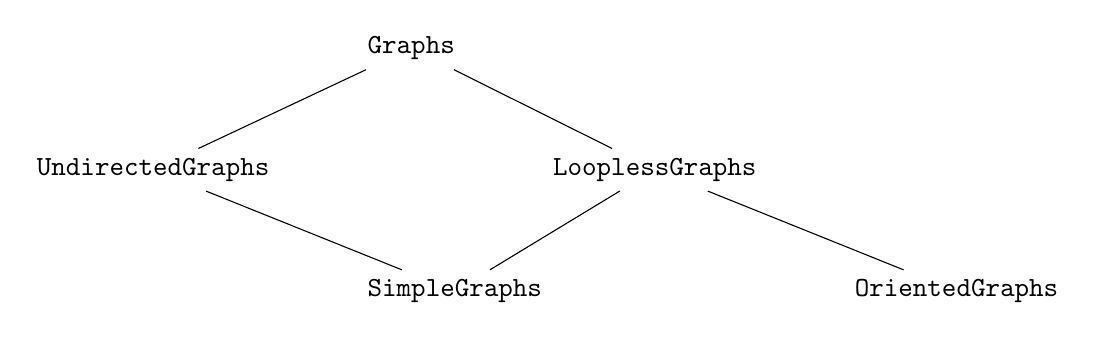
\begin{tikzpicture}[category/.style={font=\ttfamily}] \node (UG) [category]
{UndirectedGraphs}; \node (G) [category, above right=of UG] {Graphs}; \node
(SG) [category, below right=of UG] {SimpleGraphs}; \node (LG) [category, below
right=of G] {LooplessGraphs}; \node (OG) [category, below right=of LG]
{OrientedGraphs}; \draw (UG) -- (G) -- (LG) -- (OG); \draw (UG) -- (SG) --
(LG); \end{tikzpicture}   

The most general of these categories is \texttt{Graphs}\index{Graphs@\texttt{Graphs}}: every graph in \textsf{YAGS} belongs to some category and, by inclusion, every graph belongs to the
category \texttt{Graphs}. By definition a graph in \texttt{Graphs} may contain loops\index{loops}, arrows\index{arrows} and edges\index{edges} (which in \textsf{YAGS} are exactly the same as two opposite arrows); another way to say it, is that a
graph is anything that can be represented as a binary matrix (its adjacency
matrix). In particular, no multiple/parallel edges/arrows are allowed in a
graph in \textsf{YAGS}. Likewise, each of the \textsf{YAGS}'s graph categories have their own characteristic properties: 

\begin{center}
\begin{tabular}{ll}\texttt{Graphs}&
May contain loops, arrows and edges.\\
\texttt{UndirectedGraphs}\index{UndirectedGraphs@\texttt{UndirectedGraphs}}&
Can not contain plain arrows (only edges and loops).\\
\texttt{LooplessGraphs}\index{LooplessGraphs@\texttt{LooplessGraphs}}&
Can not contain loops (only arrows and edges).\\
\texttt{SimpleGraphs}\index{SimpleGraphs@\texttt{SimpleGraphs}}&
Can not contain loops nor arrows (only edges).\\
\texttt{OrientedGraphs}\index{OrientedGraphs@\texttt{OrientedGraphs}}&
Can not contain edges nor loops (only arrows).\\
\end{tabular}\\[2mm]
\end{center}

 

Graph categories simplify things for users: for example in the category \texttt{SimpleGraphs}, a \emph{complete graph} may be defined as a graph containing ``all possible edges'' among their vertices, but ``all possible edges'' in the category \texttt{Graphs} includes the loops, while in the category \texttt{OrientedGraphs}, it can only contain one arrow for each pair of vertices. 

The graph category used for constructing graphs forbids you to add a loop
accidentally or to forget to include one of the arrows that constitute an edge
in a simple graph: Every graph created in \textsf{YAGS} is forced to comply with its graph category's characteristic properties. 

\textsf{YAGS} supports several mechanisms to carefully control the graphs categories used to
construct your graphs. These are explained in the following sections. 
\section{\textcolor{Chapter }{The Default Graph Category}}\label{thedefaulgraphcategory}
\logpage{[ 4, 1, 0 ]}
\hyperdef{L}{X814CBBB3834F75F2}{}
{
  

The \texttt{DefaultGraphCategory}\index{DefaultGraphCategory@\texttt{DefaultGraphCategory}} controls (in the absence of other indications) the graph category to which the
new graphs belong. It can not be changed directly as if it were a normal
variable, instead, it can be changed by the method \texttt{SetDefaultGraphCategory} (\ref{SetDefaultGraphCategory})\index{SetDefaultGraphCategory@\texttt{SetDefaultGraphCategory}} 

 
\begin{Verbatim}[commandchars=!@|,fontsize=\small,frame=single,label=Example]
  !gapprompt@gap>| !gapinput@DefaultGraphCategory;|
  <Category "SimpleGraphs">
  !gapprompt@gap>| !gapinput@SetDefaultGraphCategory(OrientedGraphs);|
  !gapprompt@gap>| !gapinput@DefaultGraphCategory;                   |
  <Category "OrientedGraphs">
  !gapprompt@gap>| !gapinput@DefaultGraphCategory:=LooplessGraphs;|
  Error, Variable: 'DefaultGraphCategory' is read only
\end{Verbatim}
 

The effect on the constructed graphs is very noticeable: look at the
adjacencies of these graphs: 

 
\begin{Verbatim}[commandchars=!@|,fontsize=\small,frame=single,label=Example]
  !gapprompt@gap>| !gapinput@SetDefaultGraphCategory(Graphs);CompleteGraph(4);|
  Graph( Category := Graphs, Order := 4, Size := 16, Adjacencies := 
  [ [ 1, 2, 3, 4 ], [ 1, 2, 3, 4 ], [ 1, 2, 3, 4 ], [ 1, 2, 3, 4 ] ] )
  !gapprompt@gap>| !gapinput@SetDefaultGraphCategory(LooplessGraphs);CompleteGraph(4);|
  Graph( Category := LooplessGraphs, Order := 4, Size := 
  12, Adjacencies := [ [ 2, 3, 4 ], [ 1, 3, 4 ], [ 1, 2, 4 ], 
    [ 1, 2, 3 ] ] )
  !gapprompt@gap>| !gapinput@SetDefaultGraphCategory(UndirectedGraphs);CompleteGraph(4);      |
  Graph( Category := UndirectedGraphs, Order := 4, Size := 
  10, Adjacencies := [ [ 1, 2, 3, 4 ], [ 1, 2, 3, 4 ], [ 1, 2, 3, 4 ], 
    [ 1, 2, 3, 4 ] ] )
  !gapprompt@gap>| !gapinput@SetDefaultGraphCategory(OrientedGraphs);CompleteGraph(4);  |
  Graph( Category := OrientedGraphs, Order := 4, Size := 
  6, Adjacencies := [ [ 2, 3, 4 ], [ 3, 4 ], [ 4 ], [  ] ] )
  !gapprompt@gap>| !gapinput@SetDefaultGraphCategory(SimpleGraphs);CompleteGraph(4);  |
  Graph( Category := SimpleGraphs, Order := 4, Size := 
  6, Adjacencies := [ [ 2, 3, 4 ], [ 1, 3, 4 ], [ 1, 2, 4 ], 
    [ 1, 2, 3 ] ] )
\end{Verbatim}
 

When constructing a graph, \textsf{YAGS} always forces the new graphs to comply with its category, hence, in the case
of \texttt{OrientedGraphs} in the previous example, it has to remove one of the arrows conforming the
edge for each pair of vertices of the graph. Sometimes it may not be evident
which arrow will \textsf{YAGS} choose to remove, but in general, \textsf{YAGS} tries to make sense: 

 
\begin{Verbatim}[commandchars=!@|,fontsize=\small,frame=single,label=Example]
  !gapprompt@gap>| !gapinput@SetDefaultGraphCategory(OrientedGraphs);|
  !gapprompt@gap>| !gapinput@CycleGraph(4); PathGraph(4); GraphByWalks([1..5],[3,5,1]);|
  Graph( Category := OrientedGraphs, Order := 4, Size := 
  4, Adjacencies := [ [ 2 ], [ 3 ], [ 4 ], [ 1 ] ] )
  Graph( Category := OrientedGraphs, Order := 4, Size := 
  3, Adjacencies := [ [ 2 ], [ 3 ], [ 4 ], [  ] ] )
  Graph( Category := OrientedGraphs, Order := 5, Size := 
  6, Adjacencies := [ [ 2 ], [ 3 ], [ 4, 5 ], [ 5 ], [ 1 ] ] )
  !gapprompt@gap>| !gapinput@SetDefaultGraphCategory(SimpleGraphs);                    |
  !gapprompt@gap>| !gapinput@CycleGraph(4); PathGraph(4); GraphByWalks([1..5],[3,5,1]);|
  Graph( Category := SimpleGraphs, Order := 4, Size := 
  4, Adjacencies := [ [ 2, 4 ], [ 1, 3 ], [ 2, 4 ], [ 1, 3 ] ] )
  Graph( Category := SimpleGraphs, Order := 4, Size := 
  3, Adjacencies := [ [ 2 ], [ 1, 3 ], [ 2, 4 ], [ 3 ] ] )
  Graph( Category := SimpleGraphs, Order := 5, Size := 
  6, Adjacencies := [ [ 2, 5 ], [ 1, 3 ], [ 2, 4, 5 ], [ 3, 5 ], 
    [ 1, 3, 4 ] ] )
\end{Verbatim}
 

Therefore, if you always work with \texttt{SimpleGraphs}, \textsf{YAGS} defaults are perfect for you. If, in the other hand you always work with \texttt{OrientedGraphs} (also known as \emph{digraphs}\index{digraphs}), you probably would want to start all your sessions by changing the default
graph category to that... or even better, you may want to create a startup
file that does that automatically every time you start a \textsf{YAGS} session. 

On the other hand, your work may involve graphs from more than one graph
category. In such a case, it is advisable to continue reading all of this
chapter. }

 
\section{\textcolor{Chapter }{The Target Graph Category}}\label{thetargetgraphcategory}
\logpage{[ 4, 2, 0 ]}
\hyperdef{L}{X7871B6627DE80FF8}{}
{
  

The default graph category is only part of the story. When constructing new
graphs from existing ones, it may be natural to construct the new graph in the
least common category that contains the original graphs, regardless of the \texttt{DefaultGraphCategory}. 

For instance, if we have graphs \texttt{g} and \texttt{h} that belong to the categories of \texttt{SimpleGraphs} and \texttt{OrientedGraphs} (respectively), then a new graph which is the \texttt{BoxTimesProduct} (also known as the \emph{strong product}\index{strong product}) of them, should belong to the least common category of both, namely to the \texttt{LooplessGraphs} category (see the diagram at the beginning of the chapter). This is what \textsf{YAGS} does: 

 
\begin{Verbatim}[commandchars=!@|,fontsize=\small,frame=single,label=Example]
  !gapprompt@gap>| !gapinput@SetDefaultGraphCategory(SimpleGraphs);|
  !gapprompt@gap>| !gapinput@g:=PathGraph(4);|
  Graph( Category := SimpleGraphs, Order := 4, Size := 
  3, Adjacencies := [ [ 2 ], [ 1, 3 ], [ 2, 4 ], [ 3 ] ] )
  !gapprompt@gap>| !gapinput@SetDefaultGraphCategory(OrientedGraphs);|
  !gapprompt@gap>| !gapinput@h:=PathGraph(4);                                |
  Graph( Category := OrientedGraphs, Order := 4, Size := 
  3, Adjacencies := [ [ 2 ], [ 3 ], [ 4 ], [  ] ] )
  !gapprompt@gap>| !gapinput@SetDefaultGraphCategory(UndirectedGraphs);|
  !gapprompt@gap>| !gapinput@s:=BoxTimesProduct(g,h);|
  Graph( Category := LooplessGraphs, Order := 16, Size := 
  54, Adjacencies := [ [ 2, 5, 6 ], [ 3, 6, 7 ], [ 4, 7, 8 ], [ 8 ], 
    [ 1, 2, 6, 9, 10 ], [ 2, 3, 7, 10, 11 ], [ 3, 4, 8, 11, 12 ], 
    [ 4, 12 ], [ 5, 6, 10, 13, 14 ], [ 6, 7, 11, 14, 15 ], 
    [ 7, 8, 12, 15, 16 ], [ 8, 16 ], [ 9, 10, 14 ], [ 10, 11, 15 ], 
    [ 11, 12, 16 ], [ 12 ] ] )
  !gapprompt@gap>| !gapinput@s in UndirectedGraphs; s in LooplessGraphs;|
  false
  true
  !gapprompt@gap>| !gapinput@DefaultGraphCategory;|
  <Category "UndirectedGraphs">
\end{Verbatim}
 

Exactly how does \textsf{YAGS} decide this? Well, with very few and evident exceptions (such as \texttt{Orientations} (\ref{Orientations})), \textsf{YAGS}'s functions that construct graphs, always calls internally the function \texttt{TargetGraphCategory} (\ref{TargetGraphCategory}), and passes to it those of the original parameters which are graphs. 

\texttt{TargetGraphCategory} returns the graph category indicated by \textsf{GAP}'s \emph{options stack} if any (see the next section), else it returns the least common category
containing all of its parameters if any, or else (if it is called without
parameters), \texttt{TargetGraphCategory} returns the \texttt{DefaultGraphCategory}. }

 
\section{\textcolor{Chapter }{Changing the Target Graph Category in Place}}\label{changingthetargetgraphscategorytemporaly}
\logpage{[ 4, 3, 0 ]}
\hyperdef{L}{X8656BC6F81A1165D}{}
{
  

\textsf{GAP} provides a wonderful feature named \emph{options stack}\index{options stack}. Consult \textsf{GAP}'s documentation on the topic for a full explanation. For \textsf{YAGS} purposes, the short story is that you may specify the desired graph category
directly in the same command used to construct the graph without the need to
change the default graph category as in the following example: 

 
\begin{Verbatim}[commandchars=!@|,fontsize=\small,frame=single,label=Example]
  !gapprompt@gap>| !gapinput@SetDefaultGraphCategory(Graphs);      |
  !gapprompt@gap>| !gapinput@DefaultGraphCategory;           |
  <Category "Graphs">
  !gapprompt@gap>| !gapinput@g1:=CompleteGraph(4);|
  Graph( Category := Graphs, Order := 4, Size := 16, Adjacencies := 
  [ [ 1, 2, 3, 4 ], [ 1, 2, 3, 4 ], [ 1, 2, 3, 4 ], [ 1, 2, 3, 4 ] ] )
  !gapprompt@gap>| !gapinput@DefaultGraphCategory;|
  <Category "Graphs">
  !gapprompt@gap>| !gapinput@g2:=CompleteGraph(4:GraphCategory:=SimpleGraphs);  |
  Graph( Category := SimpleGraphs, Order := 4, Size := 
  6, Adjacencies := [ [ 2, 3, 4 ], [ 1, 3, 4 ], [ 1, 2, 4 ], 
    [ 1, 2, 3 ] ] )
  !gapprompt@gap>| !gapinput@DefaultGraphCategory;                            |
  <Category "Graphs">
  !gapprompt@gap>| !gapinput@g3:=CompleteGraph(4:GraphCategory:=OrientedGraphs);      |
  Graph( Category := OrientedGraphs, Order := 4, Size := 
  6, Adjacencies := [ [ 2, 3, 4 ], [ 3, 4 ], [ 4 ], [  ] ] )
  !gapprompt@gap>| !gapinput@DefaultGraphCategory;|
  <Category "Graphs">
  !gapprompt@gap>| !gapinput@h:=DisjointUnion(g2,g3);                                |
  Graph( Category := LooplessGraphs, Order := 8, Size := 
  18, Adjacencies := [ [ 2, 3, 4 ], [ 1, 3, 4 ], [ 1, 2, 4 ], 
    [ 1, 2, 3 ], [ 6, 7, 8 ], [ 7, 8 ], [ 8 ], [  ] ] )
  !gapprompt@gap>| !gapinput@DefaultGraphCategory;                                     |
  <Category "Graphs">
  !gapprompt@gap>| !gapinput@h2:=DisjointUnion(g2,g3:GraphCategory:=UndirectedGraphs);|
  Graph( Category := UndirectedGraphs, Order := 8, Size := 
  12, Adjacencies := [ [ 2, 3, 4 ], [ 1, 3, 4 ], [ 1, 2, 4 ], 
    [ 1, 2, 3 ], [ 6, 7, 8 ], [ 5, 7, 8 ], [ 5, 6, 8 ], [ 5, 6, 7 ] ] )
  !gapprompt@gap>| !gapinput@DefaultGraphCategory;                                    |
  <Category "Graphs">
\end{Verbatim}
 This method of specifying the desired category is useful to copy a graph from
one category to another using \texttt{CopyGraph} (\ref{CopyGraph}): 

 
\begin{Verbatim}[commandchars=!@|,fontsize=\small,frame=single,label=Example]
  !gapprompt@gap>| !gapinput@SetDefaultGraphCategory(SimpleGraphs);|
  !gapprompt@gap>| !gapinput@g:=PathGraph(4);|
  Graph( Category := SimpleGraphs, Order := 4, Size := 
  3, Adjacencies := [ [ 2 ], [ 1, 3 ], [ 2, 4 ], [ 3 ] ] )
  !gapprompt@gap>| !gapinput@h:=CopyGraph(g:GraphCategory:=OrientedGraphs);|
  Graph( Category := OrientedGraphs, Order := 4, Size := 
  3, Adjacencies := [ [ 2 ], [ 3 ], [ 4 ], [  ] ] )
\end{Verbatim}
 }

 }

 
\chapter{\textcolor{Chapter }{Morphisms of Graphs}}\label{morphismsofgraphs}
\logpage{[ 5, 0, 0 ]}
\hyperdef{L}{X7AB9CE86793A0114}{}
{
  
\section{\textcolor{Chapter }{A Quick Start}}\label{aquickstart}
\logpage{[ 5, 1, 0 ]}
\hyperdef{L}{X815230D9851D5961}{}
{
  

A \emph{morphism of graphs}\index{morphisms of graphs}\index{morphisms} $f:G\rightarrow H$ (Also known as \emph{homomorphisms}\index{homomorphisms}) is a function from the vertex set of one graph to the vertex set of another, $f:V(G)\rightarrow V(H)$, such that some properties (adjacency for instance) are preserved. In \textsf{YAGS} such a function is represented by a list \texttt{F=[f(1),f(2),...f(n)]}. For instance, the list \texttt{F=[2,3,4,3]} represents a morphism that maps vertex 1 of \texttt{G} onto vertex 2 of \texttt{H} and also maps 2 to 3, 3 to 4 and 4 to 3. In this example, \texttt{F} implicitly says that \texttt{G} has exactly 4 vertices and that \texttt{H} has at least 4 vertices. 

\textsf{YAGS} has a very rich and flexible set of operations to deal with \emph{graph morphisms}\index{graph morphisms} which we describe in the next sections. All these operations report progress
at \texttt{InfoLevel} 3 (see \ref{YAGSInfo.InfoClass} and Section \ref{debuggingbacktracks}). 

Here we describe only the most used ones. The operations dealing with
morphisms are organized in triplets, like the following one: 

 \begin{center}
\begin{tabular}{l}\texttt{FullMonoMorphism(G,H)} \index{FullMonoMorphism@\texttt{FullMonoMorphism}}\\
\texttt{FullMonoMorphisms(G,H)} \index{FullMonoMorphisms@\texttt{FullMonoMorphisms}}\\
\texttt{NextFullMonoMorphism(G,H,F)} \index{NextFullMonoMorphism@\texttt{NextFullMonoMorphism}}\\
\end{tabular}\\[2mm]
\end{center}

 

All three of these operations refer to the same kind of morphisms, $f$, which are \texttt{Morphisms} (the image of an edge is an edge), \texttt{Mono} (vertex-injective) and \texttt{Full} (i.e. $f(x)f(y) \in E(H) \Rightarrow \exists x'y'\in E(G)$ with $ f(x'y')=f(x)f(y)$). The first two operations simply return either \emph{one} or \emph{all} the morphisms between two given graphs: 

 
\begin{Verbatim}[commandchars=!@|,fontsize=\small,frame=single,label=Example]
  !gapprompt@gap>| !gapinput@p3:=PathGraph(3);c4:=CycleGraph(4);|
  Graph( Category := SimpleGraphs, Order := 3, Size := 
  2, Adjacencies := [ [ 2 ], [ 1, 3 ], [ 2 ] ] )
  Graph( Category := SimpleGraphs, Order := 4, Size := 
  4, Adjacencies := [ [ 2, 4 ], [ 1, 3 ], [ 2, 4 ], [ 1, 3 ] ] )
  !gapprompt@gap>| !gapinput@FullMonoMorphism(p3,c4); |
  [ 1, 2, 3 ]
  !gapprompt@gap>| !gapinput@FullMonoMorphisms(p3,c4);|
  [ [ 1, 2, 3 ], [ 1, 4, 3 ], [ 2, 1, 4 ], [ 2, 3, 4 ], [ 3, 2, 1 ], 
    [ 3, 4, 1 ], [ 4, 1, 2 ], [ 4, 3, 2 ] ]
\end{Verbatim}
 

The third operation, \texttt{NextFullMonoMorphism} receives as parameters, besides the two given graphs, a \emph{partial morphism}\index{partial morphism} \texttt{F}. As you may have guessed a partial morphism is any prefix of a morphism, so
in case \texttt{[ 1, 2, 3 ]} is a morphism, it follows that \texttt{[ 1, 2, 3 ]}, \texttt{[ 1, 2 ]}, \texttt{[ 1 ]} and \texttt{[ ]} are partial morphisms. 

Our operation \texttt{NextFullMonoMorphism} then, returns the next morphism\index{next morphism}, then one following the given partial morphism \texttt{F} in lexicographic order. It also stores this next morphism in the variable \texttt{F} so we can iteratively call \texttt{NextFullMonoMorphism} to obtain all morphisms one by one: 

 
\begin{Verbatim}[commandchars=!@|,fontsize=\small,frame=single,label=Example]
  !gapprompt@gap>| !gapinput@p3:=PathGraph(3);;c4:=CycleGraph(4);;|
  !gapprompt@gap>| !gapinput@f:=[3,4];;NextFullMonoMorphism(p3,c4,f);|
  [ 3, 4, 1 ]
  !gapprompt@gap>| !gapinput@f;|
  [ 3, 4, 1 ]
  !gapprompt@gap>| !gapinput@NextFullMonoMorphism(p3,c4,f);          |
  [ 4, 1, 2 ]
  !gapprompt@gap>| !gapinput@f;                            |
  [ 4, 1, 2 ]
  !gapprompt@gap>| !gapinput@NextFullMonoMorphism(p3,c4,f);|
  [ 4, 3, 2 ]
  !gapprompt@gap>| !gapinput@NextFullMonoMorphism(p3,c4,f);|
  fail
  !gapprompt@gap>| !gapinput@f;                            |
  [ fail ]
  !gapprompt@gap>| !gapinput@NextFullMonoMorphism(p3,c4,f);|
  [ 1, 2, 3 ]
  !gapprompt@gap>| !gapinput@NextFullMonoMorphism(p3,c4,f);|
  [ 1, 4, 3 ]
  !gapprompt@gap>| !gapinput@f:=[];                        |
  [  ]
  !gapprompt@gap>| !gapinput@NextFullMonoMorphism(p3,c4,f);|
  [ 1, 2, 3 ]
  !gapprompt@gap>| !gapinput@NextFullMonoMorphism(p3,c4,f);|
  [ 1, 4, 3 ]
\end{Verbatim}
 

Note that \texttt{f:=[ ]} and \texttt{f:=[ fail ]} are always considered partial morphisms; these are useful to compute the first
morphism and to report when there are no more morphisms to find. Please note
that \texttt{NextFullMonoMorphism} will not check whether the given partial morphism is actually a partial
morphism. This is done this way for efficiency, since actually both \texttt{FullMonoMorphism} and \texttt{FullMonoMorphisms} are implemented in terms of \texttt{NextFullMonoMorphism}. 

\texttt{NextFullMonoMorphism} is useful when the set of all morphisms from $G$ to $H$ is too big: This way, given enough time, we can process all of the morphisms
one by one even if the set of all morphisms does not fit in memory. 

The reader, may have noticed that these operations are precisely what is
needed to implement \texttt{IsInducedSubgraph}\index{IsInducedSubgraph}: 

 
\begin{Verbatim}[commandchars=!@|,fontsize=\small,frame=single,label=Example]
  !gapprompt@gap>| !gapinput@IsInducedSubgraph:=function(h,g)                                        |
  !gapprompt@>| !gapinput@return FullMonoMorphism(h,g)<>fail; end; |
  function( h, g ) ... end
  !gapprompt@gap>| !gapinput@IsInducedSubgraph(PathGraph(3),CycleGraph(4));|
  true
  !gapprompt@gap>| !gapinput@IsInducedSubgraph(PathGraph(4),CycleGraph(4));|
  false
\end{Verbatim}
 

If your morphisms of choice are not \texttt{Full} nor \texttt{Mono}, you can simply use: \begin{center}
\begin{tabular}{l}\texttt{Morphism(G,H)} \index{Morphism@\texttt{Morphism}}\\
\texttt{Morphisms(G,H)} \index{Morphisms@\texttt{Morphisms}}\\
\texttt{NextMorphism(G,H,F)} \index{NextMorphism@\texttt{NextMorphism}}\\
\end{tabular}\\[2mm]
\end{center}

 just like we did with the previous triplet of operations. 

 
\begin{Verbatim}[commandchars=!@|,fontsize=\small,frame=single,label=Example]
  !gapprompt@gap>| !gapinput@Morphism(PathGraph(3),CycleGraph(4)); |
  [ 1, 2, 1 ]
  !gapprompt@gap>| !gapinput@Morphisms(PathGraph(3),CycleGraph(4));|
  [ [ 1, 2, 1 ], [ 1, 2, 3 ], [ 1, 4, 1 ], [ 1, 4, 3 ], [ 2, 1, 2 ], 
    [ 2, 1, 4 ], [ 2, 3, 2 ], [ 2, 3, 4 ], [ 3, 2, 1 ], [ 3, 2, 3 ], 
    [ 3, 4, 1 ], [ 3, 4, 3 ], [ 4, 1, 2 ], [ 4, 1, 4 ], [ 4, 3, 2 ], 
    [ 4, 3, 4 ] ]
  !gapprompt@gap>| !gapinput@f:=[4,3];NextMorphism(PathGraph(3),CycleGraph(4),f);    |
  [ 4, 3 ]
  [ 4, 3, 2 ]
  !gapprompt@gap>| !gapinput@NextMorphism(PathGraph(3),CycleGraph(4),f);         |
  [ 4, 3, 4 ]
  !gapprompt@gap>| !gapinput@NextMorphism(PathGraph(3),CycleGraph(4),f);|
  fail
  !gapprompt@gap>| !gapinput@NextMorphism(PathGraph(3),CycleGraph(4),f);|
  [ 1, 2, 1 ]
\end{Verbatim}
 Also, this particular type of morphisms is what we need to implement \texttt{IsKColorable}\index{IsKColorable}: 

 
\begin{Verbatim}[commandchars=!@|,fontsize=\small,frame=single,label=Example]
  !gapprompt@gap>| !gapinput@IsKColorable:=function(g,k) |
  !gapprompt@>| !gapinput@return Morphism(g,CompleteGraph(k))<>fail; end;|
  function( g, k ) ... end
  !gapprompt@gap>| !gapinput@IsKColorable(CycleGraph(6),2);|
  true
  !gapprompt@gap>| !gapinput@IsKColorable(CycleGraph(5),2);|
  false
  !gapprompt@gap>| !gapinput@IsKColorable(CycleGraph(5),3);|
  true
\end{Verbatim}
 The full list of predefined types of morphisms that \textsf{YAGS} knows about is explained in the next section. }

 
\section{\textcolor{Chapter }{Predefined Types of Morphisms}}\label{predefinedtypesofmorphisms}
\logpage{[ 5, 2, 0 ]}
\hyperdef{L}{X7C6AE3D882EEFFFF}{}
{
  

Following the same organization of operations in triplets as explained in the
previous section, we present now the full list of \textsf{YAGS}'s operations for predefined types of morphisms. The operations that start
with a hash mark (\#) are not yet implemented, but they are there as a place
holders for a future implementation. \index{NextMetricMorphism@\texttt{NextMetricMorphism}}\index{NextEpiMetricMorphism@\texttt{NextEpiMetricMorphism}}\index{NextMonoMorphism@\texttt{NextMonoMorphism}}\index{NextFullMonoMorphism@\texttt{NextFullMonoMorphism}}\index{NextBiMorphism@\texttt{NextBiMorphism}}\index{NextFullBiMorphism@\texttt{NextFullBiMorphism}}\index{NextCompleteEpiWeakMorphism@\texttt{NextCompleteEpiWeakMorphism}}\index{NextCompleteEpiMorphism@\texttt{NextCompleteEpiMorphism}}\index{NextCompleteWeakMorphism@\texttt{NextCompleteWeakMorphism}}\index{NextCompleteMorphism@\texttt{NextCompleteMorphism}}\index{NextFullEpiWeakMorphism@\texttt{NextFullEpiWeakMorphism}}\index{NextFullEpiMorphism@\texttt{NextFullEpiMorphism}}\index{NextFullWeakMorphism@\texttt{NextFullWeakMorphism}}\index{NextFullMorphism@\texttt{NextFullMorphism}}\index{NextEpiWeakMorphism@\texttt{NextEpiWeakMorphism}}\index{NextEpiMorphism@\texttt{NextEpiMorphism}}\index{NextWeakMorphism@\texttt{NextWeakMorphism}}\index{NextMorphism@\texttt{NextMorphism}}\index{MetricMorphism@\texttt{MetricMorphism}}\index{EpiMetricMorphism@\texttt{EpiMetricMorphism}}\index{MonoMorphism@\texttt{MonoMorphism}}\index{FullMonoMorphism@\texttt{FullMonoMorphism}}\index{BiMorphism@\texttt{BiMorphism}}\index{FullBiMorphism@\texttt{FullBiMorphism}}\index{CompleteEpiWeakMorphism@\texttt{CompleteEpiWeakMorphism}}\index{CompleteEpiMorphism@\texttt{CompleteEpiMorphism}}\index{CompleteWeakMorphism@\texttt{CompleteWeakMorphism}}\index{CompleteMorphism@\texttt{CompleteMorphism}}\index{FullEpiWeakMorphism@\texttt{FullEpiWeakMorphism}}\index{FullEpiMorphism@\texttt{FullEpiMorphism}}\index{FullWeakMorphism@\texttt{FullWeakMorphism}}\index{FullMorphism@\texttt{FullMorphism}}\index{EpiWeakMorphism@\texttt{EpiWeakMorphism}}\index{EpiMorphism@\texttt{EpiMorphism}}\index{WeakMorphism@\texttt{WeakMorphism}}\index{Morphism@\texttt{Morphism}}\index{MetricMorphisms@\texttt{MetricMorphisms}}\index{EpiMetricMorphisms@\texttt{EpiMetricMorphisms}}\index{MonoMorphisms@\texttt{MonoMorphisms}}\index{FullMonoMorphisms@\texttt{FullMonoMorphisms}}\index{BiMorphisms@\texttt{BiMorphisms}}\index{FullBiMorphisms@\texttt{FullBiMorphisms}}\index{CompleteEpiWeakMorphisms@\texttt{CompleteEpiWeakMorphisms}}\index{CompleteEpiMorphisms@\texttt{CompleteEpiMorphisms}}\index{CompleteWeakMorphisms@\texttt{CompleteWeakMorphisms}}\index{CompleteMorphisms@\texttt{CompleteMorphisms}}\index{FullEpiWeakMorphisms@\texttt{FullEpiWeakMorphisms}}\index{FullEpiMorphisms@\texttt{FullEpiMorphisms}}\index{FullWeakMorphisms@\texttt{FullWeakMorphisms}}\index{FullMorphisms@\texttt{FullMorphisms}}\index{EpiWeakMorphisms@\texttt{EpiWeakMorphisms}}\index{EpiMorphisms@\texttt{EpiMorphisms}}\index{WeakMorphisms@\texttt{WeakMorphisms}}\index{Morphisms@\texttt{Morphisms}} 
\begin{Verbatim}[fontsize=\small,frame=single,label=Operations for predefined types of morphisms]
  NextMetricMorphism(G,H,F)
  NextEpiMetricMorphism(G,H,F)
  NextMonoMorphism(G,H,F)
  NextFullMonoMorphism(G,H,F)
  NextBiMorphism(G,H,F)
  NextFullBiMorphism(G,H,F)
  NextCompleteEpiWeakMorphism(G,H,F)
  NextCompleteEpiMorphism(G,H,F)
  NextCompleteWeakMorphism(G,H,F)
  NextCompleteMorphism(G,H,F)
  #NextFullEpiWeakMorphism(G,H,F)
  #NextFullEpiMorphism(G,H,F)
  #NextFullWeakMorphism(G,H,F)
  #NextFullMorphism(G,H,F)
  NextEpiWeakMorphism(G,H,F)
  NextEpiMorphism(G,H,F)
  NextWeakMorphism(G,H,F)
  NextMorphism(G,H,F)
  
  MetricMorphism(G,H)
  EpiMetricMorphism(G,H)
  MonoMorphism(G,H)
  FullMonoMorphism(G,H)
  BiMorphism(G,H)
  FullBiMorphism(G,H)
  CompleteEpiWeakMorphism(G,H)
  CompleteEpiMorphism(G,H)
  CompleteWeakMorphism(G,H)
  CompleteMorphism(G,H)
  #FullEpiWeakMorphism(G,H)
  #FullEpiMorphism(G,H)
  #FullWeakMorphism(G,H)
  #FullMorphism(G,H)
  EpiWeakMorphism(G,H)
  EpiMorphism(G,H)
  WeakMorphism(G,H)
  Morphism(G,H)
  
  MetricMorphisms(G,H)
  EpiMetricMorphisms(G,H)
  MonoMorphisms(G,H)
  FullMonoMorphisms(G,H)
  BiMorphisms(G,H)
  FullBiMorphisms(G,H)
  CompleteEpiWeakMorphisms(G,H)
  CompleteEpiMorphisms(G,H)
  CompleteWeakMorphisms(G,H)
  CompleteMorphisms(G,H)
  #FullEpiWeakMorphisms(G,H)
  #FullEpiMorphisms(G,H)
  #FullWeakMorphisms(G,H)
  #FullMorphisms(G,H)
  EpiWeakMorphisms(G,H)
  EpiMorphisms(G,H)
  WeakMorphisms(G,H)
  Morphisms(G,H)
\end{Verbatim}
 Here, several name fragments are used in a uniform way: 
\begin{itemize}
\item \texttt{Morphism}: The images of adjacent vertices are adjacent (except with prefix \texttt{Weak}). 
\item \texttt{Weak}: Weakens the notion of morphism so that it is allowed that adjacent vertices
go to equal ones. That is, a \texttt{WeakMorphism} is one where the images of \emph{adjacent-or-equal} vertices are also adjacent-or-equal. 
\item \texttt{Epi}: The morphism is vertex-surjective. 
\item \texttt{Mono}: The morphism is vertex-injective. 
\item \texttt{Bi}: The morphism is vertex-bijective. 
\item \texttt{Full}: $f(x)f(y) \in E(H) \Rightarrow \exists x'y'\in E(G)$ with $ f(x'y')=f(x)f(y)$. 
\item \texttt{Complete}: Whenever a pair of vertices \texttt{x, y} are mapped onto an edge of $H$, the pair \texttt{[x, y]} is also an edge (of $G$). 
\item \texttt{Metric}: The image of any pair of vertices are at the same distance from each other
as the original pair of vertices. 
\end{itemize}
 

All meaningful combinations of these name fragments are present in the full
list of operations for predefined types of morphisms. But note that some
combinations are, by mathematical reasons, necessarily synonyms like \texttt{FullBiMorphism = CompleteBiMorphism = MetricBiMorphism}; in such cases, only one of those names is selected for use in \textsf{YAGS}. Note also that a \texttt{FullBiMorphism} is most commonly known as an \emph{isomorphism}\index{isomorphism}. 

Indeed, \textsf{YAGS} knows about \texttt{FullBiMorphisms} and also about \texttt{IsoMorphisms}: the former is implemented together with all the other operations listed in
this section, using the general schema explained in the next section, while
the latter is implemented with different, more efficient, ad-hoc methods. \texttt{IsoMorphism} is faster than \texttt{FullBiMorphism}, but \texttt{FullBiMorphism} is part of a bigger, more flexible schema. }

 
\section{\textcolor{Chapter }{Main Procedures}}\label{mainprocedures}
\logpage{[ 5, 3, 0 ]}
\hyperdef{L}{X825944D279109FDC}{}
{
  

All the morphism operations listed in the previous section are implemented in
a uniform, semi-automatic way by means of the following triplet of operations,
which are explained in their indicated sections of the manual: \begin{center}
\begin{tabular}{l}\texttt{PropertyMorphism} (\ref{PropertyMorphism})\\
\texttt{PropertyMorphisms} (\ref{PropertyMorphisms})\\
\texttt{NextPropertyMorphism} (\ref{NextPropertyMorphism})\\
\end{tabular}\\[2mm]
\end{center}

 

In short, the relation of this triplet and the previous ones is best explained
by a few examples: 

 \begin{center}
\begin{tabular}{l|l}This operation:&
Is the same as:\\
\hline
\texttt{BiMorphism(G,H)}&
\texttt{PropertyMorphism(G,H,[CHK{\textunderscore}MONO,CHK{\textunderscore}EPI,CHK{\textunderscore}MORPH])}\\
\texttt{MetricMorphism(G,H)}&
\texttt{PropertyMorphism(G,H,[CHK{\textunderscore}METRIC,CHK{\textunderscore}MORPH])}\\
\texttt{CompleteWeakMorphisms(G,H)}&
 \texttt{PropertyMorphisms(G,H,[CHK{\textunderscore}CMPLT,CHK{\textunderscore}WEAK])}\\
\texttt{NextEpiMorphism(G,H,F)}&
 \texttt{NextPropertyMorphism(G,H,F,[CHK{\textunderscore}EPI,CHK{\textunderscore}MORPH])}\\
\end{tabular}\\[2mm]
\end{center}

 

In the previous table, there are several \emph{predefined property-checking functions}\index{property-checking functions}\index{property-checking functions!predefined}\index{predefined property-checking functions}: \texttt{CHK{\textunderscore}METRIC}\index{CHK{\textunderscore}METRIC}, \texttt{CHK{\textunderscore}CMPLT}\index{CHK{\textunderscore}CMPLT}, \texttt{CHK{\textunderscore}MONO}\index{CHK{\textunderscore}MONO}, \texttt{CHK{\textunderscore}EPI}\index{CHK{\textunderscore}EPI}, \texttt{CHK{\textunderscore}WEAK}\index{CHK{\textunderscore}WEAK} and \texttt{CHK{\textunderscore}MORPH}\index{CHK{\textunderscore}MORPH}. These are functions that receive, two graphs (\texttt{G} and \texttt{H}) and a partial morphism (\texttt{F}) as parameters and they return \texttt{true} whenever \texttt{F} is a valid (feasible) partial morphism from \texttt{G} to \texttt{H} satisfying the required property (i.e. metric, complete, mono, etc.); they all
return \texttt{false} otherwise. 

 
\begin{Verbatim}[commandchars=!@|,fontsize=\small,frame=single,label=Example]
  !gapprompt@gap>| !gapinput@CHK_MORPH;              |
  function( g1, g2, morph ) ... end
  !gapprompt@gap>| !gapinput@Print(CHK_MONO,"\n");|
  function ( g1, g2, morph )
      local  x, y;
      x := Length( morph );
      y := morph[x];
      if y in morph{[ 1 .. x - 1 ]}  then
          return false;
      fi;
      return true;
  end
  !gapprompt@gap>| !gapinput@Print(CHK_EPI,"\n"); |
  function ( g1, g2, morph )
      return Order( g2 ) - Length( Set( morph ) ) 
        <= Order( g1 ) - Length( morph );
  end
\end{Verbatim}
 

Note that \texttt{CHK{\textunderscore}MONO} assumes that only the last element in the partial morphism needs to be
verified for the sought property. This is correct in general since what \texttt{NextPropertyMorphism} does is to continually try to construct a new (longer) partial morphism from
an existing one, so the sought property was already checked in all prefixes of
the current partial morphism (The precise technique used by \texttt{NextPropertyMorphism} is known as backtracking, and it is described in the next chapter). 

It is usually required to include at least one of \texttt{CHK{\textunderscore}WEAK} or \texttt{CHK{\textunderscore}MORPH} in the list of properties to check used by the \texttt{PropertyMorphism} triplet, since otherwise, no adjacency-preserving function is ever verified
and then the resulting maps are more properly named ``functions'' rather than ``morphisms'': 
\begin{Verbatim}[commandchars=!@|,fontsize=\small,frame=single,label=Example]
  !gapprompt@gap>| !gapinput@k2:=CompleteGraph(2);;I2:=DiscreteGraph(2);;|
  !gapprompt@gap>| !gapinput@PropertyMorphisms(k2,I2,[]);|
  [ [ 1, 1 ], [ 1, 2 ], [ 2, 1 ], [ 2, 2 ] ]
\end{Verbatim}
 }

 
\section{\textcolor{Chapter }{User-Defined Types of Morphisms}}\label{userdefinedtypesofmorphisms}
\logpage{[ 5, 4, 0 ]}
\hyperdef{L}{X7A23DC0E7C318B24}{}
{
  

There is nothing special about \textsf{YAGS} predefined property-checking functions and the user may write new ones\index{property-checking functions!user-defined}\index{user-defined property-checking functions}. For example, if we would like to create a new type of weak morphism
restricting the mapping so that the image of a vertex always has a degree
greater than or equal to that of the vertex, then we could write: 

 
\begin{Verbatim}[commandchars=!@|,fontsize=\small,frame=single,label=Example]
  !gapprompt@gap>| !gapinput@checkdegree:=function(G,H,f)                |
  !gapprompt@>| !gapinput@local x,fx;                                 |
  !gapprompt@>| !gapinput@x:=Length(f);fx:=f[x];                      |
  !gapprompt@>| !gapinput@return VertexDegree(G,x)<=VertexDegree(H,fx);|
  !gapprompt@>| !gapinput@end;                                         |
  function( G, H, f ) ... end
  !gapprompt@gap>| !gapinput@NextSpecialMorphism:=function(G,H,F)                   |
  !gapprompt@>| !gapinput@return NextPropertyMorphism(G,H,F,[CHK_WEAK,checkdegree]); |
  !gapprompt@>| !gapinput@end;|
  function( G, H, F ) ... end
  !gapprompt@gap>| !gapinput@c4:=CycleGraph(4);;p4:=PathGraph(4);;F:=[];;|
  !gapprompt@gap>| !gapinput@NextSpecialMorphism(c4,p4,F);|
  [ 2, 2, 2, 2 ]
  !gapprompt@gap>| !gapinput@NextSpecialMorphism(c4,p4,F);|
  [ 2, 2, 2, 3 ]
  !gapprompt@gap>| !gapinput@NextSpecialMorphism(c4,p4,F);|
  [ 2, 2, 3, 2 ]
  !gapprompt@gap>| !gapinput@NextSpecialMorphism(c4,p4,F);|
  [ 2, 2, 3, 3 ]
  !gapprompt@gap>| !gapinput@SpecialMorphisms:=function(G,H)                     |
  !gapprompt@>| !gapinput@return PropertyMorphisms(G,H,[CHK_WEAK,checkdegree]);|
  !gapprompt@>| !gapinput@end;                                                 |
  function( G, H ) ... end
  !gapprompt@gap>| !gapinput@SpecialMorphisms(c4,p4);                             |
  [ [ 2, 2, 2, 2 ], [ 2, 2, 2, 3 ], [ 2, 2, 3, 2 ], [ 2, 2, 3, 3 ], 
    [ 2, 3, 2, 2 ], [ 2, 3, 2, 3 ], [ 2, 3, 3, 2 ], [ 2, 3, 3, 3 ], 
    [ 3, 2, 2, 2 ], [ 3, 2, 2, 3 ], [ 3, 2, 3, 2 ], [ 3, 2, 3, 3 ], 
    [ 3, 3, 2, 2 ], [ 3, 3, 2, 3 ], [ 3, 3, 3, 2 ], [ 3, 3, 3, 3 ] ]
\end{Verbatim}
 

Note that the property-checking functions must receive three parameters
(namely, two graphs \texttt{G,H} and a partial morphism \texttt{F}) and it is OK (and better for efficiency), if the function assumes that all
prefixes of the current partial morphism, already passed the test. 

Since all morphism-related operations in \textsf{YAGS} use \texttt{Backtrack} (\ref{Backtrack}), they all report progress at \texttt{InfoLevel} 3 (see \ref{YAGSInfo.InfoClass} and Section \ref{debuggingbacktracks}). This is useful to have an idea of how much additional time is needed for
the current computation to finish and it is also useful for debugging
user-defined property-checking functions. }

 }

 
\chapter{\textcolor{Chapter }{Backtracking}}\label{backtracking}
\logpage{[ 6, 0, 0 ]}
\hyperdef{L}{X82DE80EC7BC3EF58}{}
{
  

Backtracking is an algorithmic technique for \emph{searching in combinatorial spaces}\index{searching in combinatorial spaces}: For instance, when you need to find a particular function (morphism,
coloring, etc) subject to some criterion (\emph{iso}morphism, \emph{proper} coloring, etc). 

In this chapter we describe the technique and the facilities provided by \textsf{YAGS} to aid in the rapid prototyping of backtracking algorithms. This chapter is
written for the non-expert programmer, which is who can benefit the most from
these facilities. 

While the expert programmers will not have any problem designing their own
backtracking algorithms, they can still benefit from \textsf{YAGS}'s backtracking facilities since it may still be faster to
implement/test/prototype a backtracking algorithm using \textsf{YAGS}'s facilities. We recommend the expert programmer to go directly to \texttt{Backtrack} (\ref{Backtrack}) where a minimal non-trivial example (for computing derangements) is shown. 

The kind of combinatorial problems that can be addressed by backtracking are
those that can be represented by a decision tree: those where we have to make
a succession of choices to find a solution. These include problems where we
want to find: morphisms, isomorphisms, cages, colorings, cliques, Hamiltonian
cycles, walks, paths, subgraphs, and much, much more. Combinatorial problems
that can be represented by a decision tree are truly everywhere. \textsf{YAGS} backtracking facilities are provided by means of the operations \texttt{BacktrackBag(Opts,Chk,Done,Extra)} and \texttt{Backtrack(L,Opts,Chk,Done,Extra)}. 
\section{\textcolor{Chapter }{Simplest Examples: Using \texttt{Opts} and \texttt{Done}}}\label{simplestexamples}
\logpage{[ 6, 1, 0 ]}
\hyperdef{L}{X7B0345727995EB9C}{}
{
  

As a concrete example consider graph colorings: You have a set of colors, say \texttt{["red", "blue"]} and a graph, say \texttt{g:=PathGraph(3)}, whose vertices are \texttt{[1, 2, 3]}. Then a \emph{coloring}\index{coloring} is a function $f: \{1, 2, 3\} \rightarrow \{red, blue\}$, which in \textsf{YAGS} would be represented by a List \texttt{L:=[ f(1), f(2), f(3)]}. There are (obviously) eight of such colorings, which are easy to list using \texttt{BacktrackBag(Opts,Chk,Done,Extra)}: 

 
\begin{Verbatim}[commandchars=!@|,fontsize=\small,frame=single,label=Example]
  !gapprompt@gap>| !gapinput@colors:=["red","green"];|
  [ "red", "green" ]
  !gapprompt@gap>| !gapinput@BacktrackBag(colors,ReturnTrue,3,[]);|
  [ [ "red", "red", "red" ], [ "red", "red", "green" ], 
    [ "red", "green", "red" ], [ "red", "green", "green" ], 
    [ "green", "red", "red" ], [ "green", "red", "green" ], 
    [ "green", "green", "red" ], [ "green", "green", "green" ] ]
  !gapprompt@gap>| !gapinput@Length(last);|
  8
\end{Verbatim}
 

In the previous example, only two parameters of \texttt{BacktrackBag} are really used, namely: \texttt{Opts} (which stands for \emph{options}) and \texttt{Done}; when used in this way, \texttt{Opts} is simply the codomain of the sought function and \texttt{Done} is simply the size of the domain. When working with graph colorings it is
common to use numbers instead of actual colors or color names, so we could
also write even more compactly: 

 
\begin{Verbatim}[commandchars=!@|,fontsize=\small,frame=single,label=Example]
  !gapprompt@gap>| !gapinput@BacktrackBag([0,1],ReturnTrue,3,[]);|
  [ [ 0, 0, 0 ], [ 0, 0, 1 ], [ 0, 1, 0 ], [ 0, 1, 1 ], [ 1, 0, 0 ], 
    [ 1, 0, 1 ], [ 1, 1, 0 ], [ 1, 1, 1 ] ]
\end{Verbatim}
 

Sometimes you just want a few solutions and not the whole bag. This is
specially true when the bag is too huge (which is often the case since the bag
tend to grow exponentially in the size of the domain). For these cases, we
have \texttt{Backtrack(L,Opts,Chk,Done,Extra)}: 

 
\begin{Verbatim}[commandchars=!@|,fontsize=\small,frame=single,label=Example]
  !gapprompt@gap>| !gapinput@L:=[]; |
  [  ]
  !gapprompt@gap>| !gapinput@Backtrack(L,[0,1],ReturnTrue,3,[]);|
  [ 0, 0, 0 ]
  !gapprompt@gap>| !gapinput@L;|
  [ 0, 0, 0 ]
  !gapprompt@gap>| !gapinput@Backtrack(L,[0,1],ReturnTrue,3,[]);|
  [ 0, 0, 1 ]
  !gapprompt@gap>| !gapinput@L;                                 |
  [ 0, 0, 1 ]
  !gapprompt@gap>| !gapinput@L:=[1,1,0];|
  [ 1, 1, 0 ]
  !gapprompt@gap>| !gapinput@Backtrack(L,[0,1],ReturnTrue,3,[]);|
  [ 1, 1, 1 ]
  !gapprompt@gap>| !gapinput@L;                                 |
  [ 1, 1, 1 ]
  !gapprompt@gap>| !gapinput@Backtrack(L,[0,1],ReturnTrue,3,[]);|
  fail
  !gapprompt@gap>| !gapinput@L;|
  [ fail ]
\end{Verbatim}
 

\texttt{Backtrack(L,Opts,Chk,Done,Extra)} returns one solution at a time and it also stores the solution within \texttt{L}, so that \texttt{L} can be used as a starting point for the search of the next solution. Usually, \texttt{L:=[]} is used for the first search. When Calling \texttt{Backtrack(L,Opts,Chk,Done,Extra)}, \texttt{L} may also contain a \emph{partial} solution (i.e. a prefix of a solution like \texttt{L:=[ 1 ]} or \texttt{L:=[ 1, 0 ]}), however \texttt{Backtrack} will trust the user on this and it will not check that \texttt{L} is indeed a partial solution. 

\texttt{Backtrack} returns \texttt{fail} when no more solutions are available, but for technical reasons, \texttt{L} must always be a list, so \texttt{L:=[ fail ]} is the final value of \texttt{L}. 

Now, so far, the graph itself have not been used and the parameters \texttt{Chk} and \texttt{Extra} have not been explained. Both issues are addressed in the next section. }

 
\section{\textcolor{Chapter }{Full Examples: Using \texttt{Chk} and \texttt{Extra}}}\label{fullexamples}
\logpage{[ 6, 2, 0 ]}
\hyperdef{L}{X78F856F679888257}{}
{
  

In Graph Theory we are usually more interested in \emph{proper colorings}\index{proper coloring}\index{coloring@!proper} than just in colorings. A proper coloring is a coloring in which no two
adjacent vertices have the same color. We can easily accommodate the new
requirement within our backtracking operations. We are going to use \texttt{Chk} to check the fulfillment of the condition at each step in the construction of
a solution. Moreover, in order to check the new condition we certainly need
the extra information contained in the graph we are coloring. This extra
information (the graph) is passed in the \texttt{Extra} parameter. 

More generally, \texttt{Chk} is a user-provided function \texttt{Chk(L,Extra)} which receives a partial solution \texttt{L} and some extra information \texttt{Extra}; it returns \texttt{false} whenever it knows that \texttt{L} can not be completed to a full solution and it returns \texttt{true} otherwise. Note then that our backtracking operations internally call \texttt{Chk} several times during the process of constructing each solution: once each time \texttt{L} grows in length. In each call to \texttt{Chk} it is safe to assume that all proper prefixes of \texttt{L} have already been verified and approved by \texttt{Chk}. 

In our example, \texttt{L} contains the color choices already made for the first vertices: \texttt{1, 2, ... Length(L)}. It is safe to assume that all but the last choice are already checked to
satisfy the properness requirement. The last color choice so far is then the
one in \texttt{L[Length(L)]} and we have to check (within \texttt{Chk}) if it also satisfy the properness requirement. We can do it like this: 

 
\begin{Verbatim}[commandchars=!@|,fontsize=\small,frame=single,label=Example]
  !gapprompt@gap>| !gapinput@g:=PathGraph(3);;                                    |
  !gapprompt@gap>| !gapinput@chk:=function(L,g)                                   |
  !gapprompt@>| !gapinput@       local x,y;                                           |
  !gapprompt@>| !gapinput@       if L=[] then return true; fi;                        |
  !gapprompt@>| !gapinput@       x:=Length(L);                                        |
  !gapprompt@>| !gapinput@       for y in [1..x-1] do                                 |
  !gapprompt@>| !gapinput@          if IsEdge(g,[x,y]) and L[x]=L[y] then|
  !gapprompt@>| !gapinput@             return false;|
  !gapprompt@>| !gapinput@          fi;|
  !gapprompt@>| !gapinput@       od;|
  !gapprompt@>| !gapinput@       return true;|
  !gapprompt@>| !gapinput@   end;|
  function( L, g ) ... end
  !gapprompt@gap>| !gapinput@BacktrackBag([0,1],chk,Order(g),g);                     |
  [ [ 0, 1, 0 ], [ 1, 0, 1 ] ]
\end{Verbatim}
 

Now we get only two solutions, as expected. We emphasize here the fact that \texttt{Chk} is internally called by \texttt{BacktrackBag} each time \texttt{L} grows in length. Therefore (for instance) at some point the partial solution \texttt{[ 0, 0 ]} is tried and since it is found unfeasible by \texttt{Chk} is is discarded and no other partial solution with that prefix is ever tried.
This produces huge reductions in execution time as compared to the (naive)
approach of computing all the colorings first and then filtering out those
which does not satisfy the properness requirement. In particular we can
compute proper colorings for graphs where the naive approach fails: 

 
\begin{Verbatim}[commandchars=!@|,fontsize=\small,frame=single,label=Example]
  !gapprompt@gap>| !gapinput@g:=PathGraph(70);;|
  !gapprompt@gap>| !gapinput@BacktrackBag([0,1],chk,Order(g),g);|
  [ [ 0, 1, 0, 1, 0, 1, 0, 1, 0, 1, 0, 1, 0, 1, 0, 1, 0, 1, 0, 1, 0, 1, 
        0, 1, 0, 1, 0, 1, 0, 1, 0, 1, 0, 1, 0, 1, 0, 1, 0, 1, 0, 1, 0, 
        1, 0, 1, 0, 1, 0, 1, 0, 1, 0, 1, 0, 1, 0, 1, 0, 1, 0, 1, 0, 1, 
        0, 1, 0, 1, 0, 1 ], 
    [ 1, 0, 1, 0, 1, 0, 1, 0, 1, 0, 1, 0, 1, 0, 1, 0, 1, 0, 1, 0, 1, 0, 
        1, 0, 1, 0, 1, 0, 1, 0, 1, 0, 1, 0, 1, 0, 1, 0, 1, 0, 1, 0, 1, 
        0, 1, 0, 1, 0, 1, 0, 1, 0, 1, 0, 1, 0, 1, 0, 1, 0, 1, 0, 1, 0, 
        1, 0, 1, 0, 1, 0 ] ]
\end{Verbatim}
 

Of course, we can now compute proper colorings for many other graphs as well: 

 
\begin{Verbatim}[commandchars=!@|,fontsize=\small,frame=single,label=Example]
  !gapprompt@gap>| !gapinput@g:=CycleGraph(5);;                 |
  !gapprompt@gap>| !gapinput@BacktrackBag([0,1],chk,Order(g),g);|
  [  ]
  !gapprompt@gap>| !gapinput@BacktrackBag([0,1,2],chk,Order(g),g);|
  [ [ 0, 1, 0, 1, 2 ], [ 0, 1, 0, 2, 1 ], [ 0, 1, 2, 0, 1 ], 
    [ 0, 1, 2, 0, 2 ], [ 0, 1, 2, 1, 2 ], [ 0, 2, 0, 1, 2 ], 
    [ 0, 2, 0, 2, 1 ], [ 0, 2, 1, 0, 1 ], [ 0, 2, 1, 0, 2 ], 
    [ 0, 2, 1, 2, 1 ], [ 1, 0, 1, 0, 2 ], [ 1, 0, 1, 2, 0 ], 
    [ 1, 0, 2, 0, 2 ], [ 1, 0, 2, 1, 0 ], [ 1, 0, 2, 1, 2 ], 
    [ 1, 2, 0, 1, 0 ], [ 1, 2, 0, 1, 2 ], [ 1, 2, 0, 2, 0 ], 
    [ 1, 2, 1, 0, 2 ], [ 1, 2, 1, 2, 0 ], [ 2, 0, 1, 0, 1 ], 
    [ 2, 0, 1, 2, 0 ], [ 2, 0, 1, 2, 1 ], [ 2, 0, 2, 0, 1 ], 
    [ 2, 0, 2, 1, 0 ], [ 2, 1, 0, 1, 0 ], [ 2, 1, 0, 2, 0 ], 
    [ 2, 1, 0, 2, 1 ], [ 2, 1, 2, 0, 1 ], [ 2, 1, 2, 1, 0 ] ]
  !gapprompt@gap>| !gapinput@g:=Icosahedron;;                          |
  !gapprompt@gap>| !gapinput@Backtrack([],[0,1,2],chk,Order(g),g);|
  fail
  !gapprompt@gap>| !gapinput@Backtrack([],[0,1,2,3],chk,Order(g),g);|
  [ 0, 1, 2, 1, 2, 3, 3, 0, 2, 3, 0, 1 ]
\end{Verbatim}
 }

 
\section{\textcolor{Chapter }{Advanced Examples: When \texttt{Opts} and \texttt{Done} are functions}}\label{advancedexamples}
\logpage{[ 6, 3, 0 ]}
\hyperdef{L}{X800306D77D886EC6}{}
{
  

Our backtracking operations \texttt{BacktrackBag(Opts,Chk,Done,Extra)} and \texttt{Backtrack(L,Opts,Chk,Done,Extra)} are even more flexible that shown so far. In our previous examples \texttt{Opts} was always a list and \texttt{Done} was always an integer. Both can also be functions. 

When \texttt{Opts} is a function, it receives \texttt{L} and \texttt{Extra}, and then \texttt{Opts(L,Extra)} should return the list of options available to extend the partial solution \texttt{L} at that particular stage. This way the list of options can be different at
different times which is useful for instance when the union of all possible
options is too big or even unbounded. 

When \texttt{Done} is a function, it also receives \texttt{L} and \texttt{Extra}, and then \texttt{Done(L,Extra)} returns \texttt{true} whenever \texttt{L} is a full solution and it returns \texttt{false} otherwise. This is useful when not all the solutions have the same length.
Thus the number \texttt{N} we used to put in place of the function \texttt{Done(L,Extra)} is equivalent to the function \texttt{Done:=function(L,Extra) return Length(L) {\textgreater}= N; end;}. 

Also, when a number \texttt{N} is used in place of \texttt{Done}, an implicit upper bound \texttt{Length(L){\textless}= N} is added internally to \texttt{Chk}, so it is \emph{imperative} to add such an explicit bound to \texttt{Chk} when a function is used for \texttt{Done} otherwise the backtracking algorithm will try to find longer and longer
solutions without bound or end until the memory of the computer is exhausted. 

As an example, assume we want to find all the walks on 5-cycle that start at
vertex 1 and end at vertex 2 with length at most 4 (at most 5 vertices). Then
we can proceed as follows: 

 
\begin{Verbatim}[commandchars=!@|,fontsize=\small,frame=single,label=Example]
  !gapprompt@gap>| !gapinput@g:=CycleGraph(5);|
  Graph( Category := SimpleGraphs, Order := 5, Size := 
  5, Adjacencies := [ [ 2, 5 ], [ 1, 3 ], [ 2, 4 ], [ 3, 5 ], [ 1, 4 ] 
   ] )
  !gapprompt@gap>| !gapinput@opts:=function(L,g) |
  !gapprompt@>| !gapinput@            if L=[] then |
  !gapprompt@>| !gapinput@               return [1]; |
  !gapprompt@>| !gapinput@            else |
  !gapprompt@>| !gapinput@               return Adjacency(g,L[Length(L)]); |
  !gapprompt@>| !gapinput@           fi; |
  !gapprompt@>| !gapinput@   end;|
  function( L, g ) ... end
  !gapprompt@gap>| !gapinput@chk:=function(L,g) return Length(L)<= 5; end;|
  function( L, g ) ... end
  !gapprompt@gap>| !gapinput@done:=function(L,g) return L[Length(L)]=2; end;|
  function( L, g ) ... end
  !gapprompt@gap>| !gapinput@BacktrackBag(opts,chk,done,g);|
  [ [ 1, 2 ], [ 1, 2, 1, 2 ], [ 1, 2, 3, 2 ], [ 1, 5, 1, 2 ], 
    [ 1, 5, 4, 3, 2 ] ]
\end{Verbatim}
 

Finally you may wonder why only \emph{one} extra parameter \texttt{Extra} is allowed, what if I need more than one? Well, the parameter \texttt{Extra} may be any object supported by \textsf{GAP}; indeed \textsf{YAGS} only uses it to pass information to the user-defined functions \texttt{Opts(L,Extra)}, \texttt{Chk(L,Extra)} and \texttt{Done(L,Extra)}. Hence, if you need pass more than one extra parameter, say two graphs \texttt{g} and \texttt{h}, you just put them in a list (or record, etc) and pass the parameter \texttt{Extra:=[g,h]}. }

 
\section{\textcolor{Chapter }{Debugging Backtracking Algorithms.}}\label{debuggingbacktracks}
\logpage{[ 6, 4, 0 ]}
\hyperdef{L}{X7F9CE7A87E7B0111}{}
{
  

Sooner or later you will need to debug a backtracking algorithm that is not
working as expected, or at least, you would like to know how much work your
algorithm has done and how much remains to be done to decide if it is worth
waiting for an answer (since backtracking techniques easily produce algorithms
which may take eons to finish). 

All of \textsf{YAGS}'s backtracking operations report progress info at \texttt{InfoLevel} 3 to \textsf{YAGS}'s info class \texttt{YAGSInfo.InfoClass} (see \ref{YAGSInfo.InfoClass}). In short, this means that setting \texttt{SetInfoLevel(YAGSInfo.InfoClass,3);} will cause all backtracking operations to report progress information to the
console: The contents of \texttt{L} will be reported each time it grows in length. Revert to the default behavior
by setting the \texttt{InfoLevel} to 0 using \texttt{SetInfoLevel(YAGSInfo.InfoClass,0);} 

 
\begin{Verbatim}[commandchars=!@|,fontsize=\small,frame=single,label=Example]
  !gapprompt@gap>| !gapinput@SetInfoLevel(YAGSInfo.InfoClass,3); |
  !gapprompt@gap>| !gapinput@BacktrackBag([0,1],ReturnTrue,3,[]);|
  #I [  ]
  #I [ 0 ]
  #I [ 0, 0 ]
  #I [ 0, 0, 0 ]
  #I [ 0, 0, 1 ]
  #I [ 0, 1 ]
  #I [ 0, 1, 0 ]
  #I [ 0, 1, 1 ]
  #I [ 1 ]
  #I [ 1, 0 ]
  #I [ 1, 0, 0 ]
  #I [ 1, 0, 1 ]
  #I [ 1, 1 ]
  #I [ 1, 1, 0 ]
  #I [ 1, 1, 1 ]
  [ [ 0, 0, 0 ], [ 0, 0, 1 ], [ 0, 1, 0 ], [ 0, 1, 1 ], [ 1, 0, 0 ], 
  [ 1, 0, 1 ], [ 1, 1, 0 ], [ 1, 1, 1 ] ]
  !gapprompt@gap>| !gapinput@SetInfoLevel(YAGSInfo.InfoClass,0);|
  !gapprompt@gap>| !gapinput@BacktrackBag([0,1],ReturnTrue,3,[]);|
  [ [ 0, 0, 0 ], [ 0, 0, 1 ], [ 0, 1, 0 ], [ 0, 1, 1 ], [ 1, 0, 0 ], 
    [ 1, 0, 1 ], [ 1, 1, 0 ], [ 1, 1, 1 ] ]
\end{Verbatim}
 

The output of the progress info may be redirected to a file or character
device by setting the variable \texttt{YAGSInfo.InfoOutput} (\ref{YAGSInfo.InfoOutput}) accordingly. 

The information in this section about progress reporting applies to all \textsf{YAGS} functions that internally use \texttt{Backtrack} (\ref{Backtrack}) or \texttt{BacktrackBag} (\ref{BacktrackBag}), namely \texttt{CompletesOfGivenOrder} (\ref{CompletesOfGivenOrder}), \texttt{Orientations} (\ref{Orientations}) and all morphism-related operations in Chapter \ref{morphismsofgraphs}. }

 }

 

\appendix


\chapter{\textcolor{Chapter }{\textsf{YAGS} Functions by Topic}}\label{alltopic}
\logpage{[ "A", 0, 0 ]}
\hyperdef{L}{X80E1CB8A7907178D}{}
{
  

A complete list of all \textsf{YAGS}'s functions organized by topic. 
\section{\textcolor{Chapter }{Most Common Functions}}\label{tmostcommonfunctions}
\logpage{[ "A", 1, 0 ]}
\hyperdef{L}{X7C2382C381CC357C}{}
{
  
\begin{itemize}
\item \texttt{AddEdges( \mbox{\texttt{\mdseries\slshape G}}, \mbox{\texttt{\mdseries\slshape E}} )}\\
 Returns a new graph obtained from \mbox{\texttt{\mdseries\slshape G}} by adding the list of edges in \mbox{\texttt{\mdseries\slshape E}}. (\ref{AddEdges}) 
\item \texttt{Adjacency( \mbox{\texttt{\mdseries\slshape G}}, \mbox{\texttt{\mdseries\slshape x}} )}\\
 Returns the list of vertices in \mbox{\texttt{\mdseries\slshape G}} which are adjacent to vertex \mbox{\texttt{\mdseries\slshape x}}. (\ref{Adjacency}) 
\item \texttt{AutomorphismGroup( \mbox{\texttt{\mdseries\slshape G}} )}\\
 Returns the automorphism group of graph \mbox{\texttt{\mdseries\slshape G}}. A synonym is \texttt{AutGroupGraph( \mbox{\texttt{\mdseries\slshape G}} )}. (\ref{AutomorphismGroup}) 
\item \texttt{BoxProduct( \mbox{\texttt{\mdseries\slshape G}}, \mbox{\texttt{\mdseries\slshape H}} );}\\
 Returns the box product (or Cartesian product) \mbox{\texttt{\mdseries\slshape G}}$\Box$\mbox{\texttt{\mdseries\slshape H}} of graphs \mbox{\texttt{\mdseries\slshape G}} and \mbox{\texttt{\mdseries\slshape H}}. (\ref{BoxProduct}) 
\item \texttt{BoxTimesProduct( \mbox{\texttt{\mdseries\slshape G}}, \mbox{\texttt{\mdseries\slshape H}} )}\\
 Returns the boxtimes product (or strong product) \mbox{\texttt{\mdseries\slshape G}}$\boxtimes$\mbox{\texttt{\mdseries\slshape H}} of graphs \mbox{\texttt{\mdseries\slshape G}} and \mbox{\texttt{\mdseries\slshape H}}. (\ref{BoxTimesProduct}) 
\item \texttt{Circulant( \mbox{\texttt{\mdseries\slshape n}}, \mbox{\texttt{\mdseries\slshape Jumps}} )}\\
 Returns the minimal graph invariant under the cyclic permutation $(1\;\,2\;\,\cdots\;\,n)$ such that the vertex 1 is adjacent to the vertices in \mbox{\texttt{\mdseries\slshape Jumps}}. (\ref{Circulant}) 
\item \texttt{CliqueGraph( \mbox{\texttt{\mdseries\slshape G}} )}\\
 \texttt{CliqueGraph( \mbox{\texttt{\mdseries\slshape G}}, \mbox{\texttt{\mdseries\slshape maxNumCli}} )}\\
 Returns the intersection graph of the (maximal) cliques of \mbox{\texttt{\mdseries\slshape G}}; aborts if \mbox{\texttt{\mdseries\slshape maxNumCli}} cliques are found. (\ref{CliqueGraph}) 
\item \texttt{Cliques( \mbox{\texttt{\mdseries\slshape G}} )}\\
 \texttt{Cliques( \mbox{\texttt{\mdseries\slshape G}}, \mbox{\texttt{\mdseries\slshape maxNumCli}} )}\\
 Returns the list of (maximal) cliques of \mbox{\texttt{\mdseries\slshape G}}; aborts if \mbox{\texttt{\mdseries\slshape maxNumCli}} cliques are found. (\ref{Cliques}) 
\item \texttt{ComplementGraph( \mbox{\texttt{\mdseries\slshape G}} )}\\
 Returns a new graph \mbox{\texttt{\mdseries\slshape H}} such that $V(\mbox{\texttt{\mdseries\slshape H}})=V(\mbox{\texttt{\mdseries\slshape G}})$ and $xy\in E(\mbox{\texttt{\mdseries\slshape H}}) \iff xy \not\in E(\mbox{\texttt{\mdseries\slshape G}})$. (\ref{ComplementGraph}) 
\item \texttt{CompleteGraph( \mbox{\texttt{\mdseries\slshape n}} )}\\
 Returns the graph on \mbox{\texttt{\mdseries\slshape n}} vertices having all possible edges present. (\ref{CompleteGraph}) 
\item \texttt{CompleteMultipartiteGraph( \mbox{\texttt{\mdseries\slshape n1}}, \mbox{\texttt{\mdseries\slshape n2}} [, \mbox{\texttt{\mdseries\slshape n3}} ...] )}\\
 Returns the graph with $r\geq 2$ parts of orders \mbox{\texttt{\mdseries\slshape n1}}, \mbox{\texttt{\mdseries\slshape n2}}, ... such that each vertex is adjacent exactly to all the vertices in the
other parts not containing itself. (\ref{CompleteMultipartiteGraph}) 
\item \texttt{ConnectedComponents( \mbox{\texttt{\mdseries\slshape G}} )}\\
 Returns the equivalence partition of $V(G)$ corresponding to the equivalence relation ``reachable'' in \mbox{\texttt{\mdseries\slshape G}}. (\ref{ConnectedComponents}) 
\item \texttt{CycleGraph( \mbox{\texttt{\mdseries\slshape n}} )}\\
 Returns the cyclic graph on \mbox{\texttt{\mdseries\slshape n}} vertices. (\ref{CycleGraph}) 
\item \texttt{Diameter( \mbox{\texttt{\mdseries\slshape G}} )}\\
 Returns the maximum among the distances between pairs of vertices of \mbox{\texttt{\mdseries\slshape G}}. (\ref{Diameter}) 
\item \texttt{DiscreteGraph( \mbox{\texttt{\mdseries\slshape n}} )}\\
 Returns the graph on \mbox{\texttt{\mdseries\slshape n}} vertices with no edges. (\ref{DiscreteGraph}) 
\item \texttt{DisjointUnion( \mbox{\texttt{\mdseries\slshape G}}, \mbox{\texttt{\mdseries\slshape H}} )}\\
 Returns the disjoint union of two graphs \mbox{\texttt{\mdseries\slshape G}} and \mbox{\texttt{\mdseries\slshape H}}. (\ref{DisjointUnion}) 
\item \texttt{Distance( \mbox{\texttt{\mdseries\slshape G}}, \mbox{\texttt{\mdseries\slshape x}}, \mbox{\texttt{\mdseries\slshape y}} )}\\
 Returns the minimum length of a path connecting \mbox{\texttt{\mdseries\slshape x}} to \mbox{\texttt{\mdseries\slshape y}} in \mbox{\texttt{\mdseries\slshape G}}. (\ref{Distance}) 
\item \texttt{Draw( \mbox{\texttt{\mdseries\slshape G}} )}\\
 Draws the graph \mbox{\texttt{\mdseries\slshape G}} on a new window. (\ref{Draw}) 
\item \texttt{Edges( \mbox{\texttt{\mdseries\slshape G}} )}\\
 Returns the list of edges of graph \mbox{\texttt{\mdseries\slshape G}}. (\ref{Edges}) 
\item \texttt{GraphAttributeStatistics( \mbox{\texttt{\mdseries\slshape OrderList}}, \mbox{\texttt{\mdseries\slshape ProbList}}, \mbox{\texttt{\mdseries\slshape Attribute}} )}\\
 Returns statistics for graph attribute \mbox{\texttt{\mdseries\slshape Attribute}}. (\ref{GraphAttributeStatistics}) 
\item \texttt{GraphByAdjacencies( \mbox{\texttt{\mdseries\slshape AdjList}} )}\\
 Returns a new graph having \mbox{\texttt{\mdseries\slshape AdjList}} as its list of adjacencies. (\ref{GraphByAdjacencies}) 
\item \texttt{GraphByAdjMatrix( \mbox{\texttt{\mdseries\slshape Mat}} )}\\
 Returns a new graph created from an adjacency matrix \mbox{\texttt{\mdseries\slshape Mat}}. (\ref{GraphByAdjMatrix}) 
\item \texttt{GraphByCompleteCover( \mbox{\texttt{\mdseries\slshape Cover}} )}\\
 Returns the minimal graph where the elements of \mbox{\texttt{\mdseries\slshape Cover}} are (the vertex sets of) complete subgraphs. (\ref{GraphByCompleteCover}) 
\item \texttt{GraphByEdges( \mbox{\texttt{\mdseries\slshape L}} )}\\
 Returns the minimal graph such that the pairs in \mbox{\texttt{\mdseries\slshape L}} are edges. (\ref{GraphByEdges}) 
\item \texttt{GraphByRelation( \mbox{\texttt{\mdseries\slshape V}}, \mbox{\texttt{\mdseries\slshape Rel}} )}\\
 \texttt{GraphByRelation( \mbox{\texttt{\mdseries\slshape n}}, \mbox{\texttt{\mdseries\slshape Rel}} )}\\
 Returns a new graph $G$ where $xy \in E(G)$ iff \mbox{\texttt{\mdseries\slshape Rel}}$(x,y)=$\texttt{true}. (\ref{GraphByRelation}) 
\item \texttt{GraphByWalks( \mbox{\texttt{\mdseries\slshape Walk1}}, \mbox{\texttt{\mdseries\slshape Walk2}},...)}\\
 Returns the minimal graph such that \mbox{\texttt{\mdseries\slshape Walk1}}, \mbox{\texttt{\mdseries\slshape Walk2}}, etc are walks. (\ref{GraphByWalks}) 
\item \texttt{GraphSum( \mbox{\texttt{\mdseries\slshape G}}, \mbox{\texttt{\mdseries\slshape L}} )}\\
 Returns the lexicographic sum of a list of graphs \mbox{\texttt{\mdseries\slshape L}} over a graph \mbox{\texttt{\mdseries\slshape G}}. (\ref{GraphSum}) 
\item \texttt{InducedSubgraph( \mbox{\texttt{\mdseries\slshape G}}, \mbox{\texttt{\mdseries\slshape V}} )}\\
 Returns the subgraph \mbox{\texttt{\mdseries\slshape G}} induced by the vertex set \mbox{\texttt{\mdseries\slshape V}}. (\ref{InducedSubgraph}) 
\item \texttt{InNeigh( \mbox{\texttt{\mdseries\slshape G}}, \mbox{\texttt{\mdseries\slshape x}} )}\\
 Returns the list of in-neighbors of \mbox{\texttt{\mdseries\slshape x}} in \mbox{\texttt{\mdseries\slshape G}}. (\ref{InNeigh}) 
\item \texttt{IntersectionGraph( \mbox{\texttt{\mdseries\slshape L}} )}\\
 Returns the graph $G$ where $V(G)=L$ and $XY\in E(G) \iff X\cap Y \neq \varnothing$. (\ref{IntersectionGraph}) 
\item \texttt{IsEdge( \mbox{\texttt{\mdseries\slshape G}}, \mbox{\texttt{\mdseries\slshape x}}, \mbox{\texttt{\mdseries\slshape y}} )}\\
 \texttt{IsEdge( \mbox{\texttt{\mdseries\slshape G}}, [\mbox{\texttt{\mdseries\slshape x}},\mbox{\texttt{\mdseries\slshape y}}] )}\\
 Returns \texttt{true} if \texttt{[\mbox{\texttt{\mdseries\slshape x}},\mbox{\texttt{\mdseries\slshape y}}]} is an edge of \mbox{\texttt{\mdseries\slshape G}}. (\ref{IsEdge}) 
\item \texttt{IsIsomorphicGraph( \mbox{\texttt{\mdseries\slshape G}}, \mbox{\texttt{\mdseries\slshape H}} )}\\
 Returns \texttt{true} when \mbox{\texttt{\mdseries\slshape G}} is isomorphic to \mbox{\texttt{\mdseries\slshape H}} and \texttt{false} otherwise. (\ref{IsIsomorphicGraph}) 
\item \texttt{Join( \mbox{\texttt{\mdseries\slshape G}}, \mbox{\texttt{\mdseries\slshape H}} )}\\
 Returns the disjoint union of \mbox{\texttt{\mdseries\slshape G}} and \mbox{\texttt{\mdseries\slshape H}} with all the possible edges between \mbox{\texttt{\mdseries\slshape G}} and \mbox{\texttt{\mdseries\slshape H}} added. (\ref{Join}) 
\item \texttt{LineGraph( \mbox{\texttt{\mdseries\slshape G}} )}\\
 Returns the intersection graph of the edges of \mbox{\texttt{\mdseries\slshape G}}. (\ref{LineGraph}) 
\item \texttt{Link( \mbox{\texttt{\mdseries\slshape G}}, \mbox{\texttt{\mdseries\slshape x}} )}\\
 Returns the subgraph induced in \mbox{\texttt{\mdseries\slshape G}} by the neighbors of \mbox{\texttt{\mdseries\slshape x}}. (\ref{Link}) 
\item \texttt{MaxDegree( \mbox{\texttt{\mdseries\slshape G}} )}\\
 Returns the maximum degree in graph \mbox{\texttt{\mdseries\slshape G}}. (\ref{MaxDegree}) 
\item \texttt{MinDegree( \mbox{\texttt{\mdseries\slshape G}} )}\\
 Returns the minimum degree in graph \mbox{\texttt{\mdseries\slshape G}}. (\ref{MinDegree}) 
\item \texttt{Order( \mbox{\texttt{\mdseries\slshape G}} )}\\
 Returns the number of vertices, of graph \mbox{\texttt{\mdseries\slshape G}}. (\ref{Order}) 
\item \texttt{PathGraph( \mbox{\texttt{\mdseries\slshape n}} )}\\
 Returns the path graph on \mbox{\texttt{\mdseries\slshape n}} vertices. (\ref{PathGraph}) 
\item \texttt{QuotientGraph( \mbox{\texttt{\mdseries\slshape G}}, \mbox{\texttt{\mdseries\slshape Part}} )}\\
 \texttt{QuotientGraph( \mbox{\texttt{\mdseries\slshape G}}, \mbox{\texttt{\mdseries\slshape L1}}, \mbox{\texttt{\mdseries\slshape L2}} )}\\
 Returns the quotient graph of graph \mbox{\texttt{\mdseries\slshape G}} given a vertex partition \mbox{\texttt{\mdseries\slshape Part}}, by identifying any two vertices in the same part. (\ref{QuotientGraph}) 
\item \texttt{RandomGraph( \mbox{\texttt{\mdseries\slshape n}}, \mbox{\texttt{\mdseries\slshape p}} )}\\
 \texttt{RandomGraph( \mbox{\texttt{\mdseries\slshape n}} )}\\
 Returns a random graph of order \mbox{\texttt{\mdseries\slshape n}} with edge probability $p$ (a rational in $[0,1]$). (\ref{RandomGraph}) 
\item \texttt{RemoveEdges( \mbox{\texttt{\mdseries\slshape G}}, \mbox{\texttt{\mdseries\slshape E}} )}\\
 Returns a new graph created from graph \mbox{\texttt{\mdseries\slshape G}} by removing the edges in list \mbox{\texttt{\mdseries\slshape E}}. (\ref{RemoveEdges}) 
\item \texttt{SetDefaultGraphCategory( \mbox{\texttt{\mdseries\slshape Catgy}} )}\\
 Sets the default graph category to \mbox{\texttt{\mdseries\slshape Catgy}}. (\ref{SetDefaultGraphCategory}) 
\item \texttt{Size( \mbox{\texttt{\mdseries\slshape G}} )}\\
 Returns the number of edges of graph \mbox{\texttt{\mdseries\slshape G}}. (\ref{Size}) 
\item \texttt{TimesProduct( \mbox{\texttt{\mdseries\slshape G}}, \mbox{\texttt{\mdseries\slshape H}} )}\\
 Returns the times product (or tensor product) \mbox{\texttt{\mdseries\slshape G}}$\times$\mbox{\texttt{\mdseries\slshape H}} of two graphs \mbox{\texttt{\mdseries\slshape G}} and \mbox{\texttt{\mdseries\slshape H}}. (\ref{TimesProduct}) 
\item \texttt{TrivialGraph}\\
 The one vertex graph. (\ref{TrivialGraph}) 
\item \texttt{VertexDegree( \mbox{\texttt{\mdseries\slshape G}}, \mbox{\texttt{\mdseries\slshape x}} )}\\
 Returns the degree of vertex \mbox{\texttt{\mdseries\slshape x}} in graph \mbox{\texttt{\mdseries\slshape G}}. (\ref{VertexDegree}) 
\item \texttt{VertexNames( \mbox{\texttt{\mdseries\slshape G}} )}\\
 Returns the list of names of the vertices of \mbox{\texttt{\mdseries\slshape G}}. (\ref{VertexNames}) 
\item \texttt{WheelGraph( \mbox{\texttt{\mdseries\slshape n}} )}\\
 \texttt{WheelGraph( \mbox{\texttt{\mdseries\slshape n}}, \mbox{\texttt{\mdseries\slshape r}} )}\\
 This is the cone of an \mbox{\texttt{\mdseries\slshape n}}-cycle; when present, \mbox{\texttt{\mdseries\slshape r}} is the radius of the wheel. (\ref{WheelGraph}) 
\end{itemize}
 }

 
\section{\textcolor{Chapter }{Drawing}}\label{tdrawing}
\logpage{[ "A", 2, 0 ]}
\hyperdef{L}{X7AFE6B467AB077A8}{}
{
  
\begin{itemize}
\item \texttt{Coordinates( \mbox{\texttt{\mdseries\slshape G}} )}\\
 Returns the list of coordinates of the vertices of \mbox{\texttt{\mdseries\slshape G}} if they exist; fail otherwise. (\ref{Coordinates}) 
\item \texttt{Draw( \mbox{\texttt{\mdseries\slshape G}} )}\\
 Draws the graph \mbox{\texttt{\mdseries\slshape G}} on a new window. (\ref{Draw}) 
\item \texttt{GraphToRaw( \mbox{\texttt{\mdseries\slshape FileName}}, \mbox{\texttt{\mdseries\slshape G}} )}\\
 Writes the graph \mbox{\texttt{\mdseries\slshape G}} in raw format to the file \mbox{\texttt{\mdseries\slshape FileName}}. (\ref{GraphToRaw}) 
\item \texttt{GraphUpdateFromRaw( \mbox{\texttt{\mdseries\slshape FileName}}, \mbox{\texttt{\mdseries\slshape G}} )}\\
 Updates the coordinates of \mbox{\texttt{\mdseries\slshape G}} from a file \mbox{\texttt{\mdseries\slshape FileName}} in raw format. (\ref{GraphUpdateFromRaw}) 
\item \texttt{SetCoordinates( \mbox{\texttt{\mdseries\slshape G}}, \mbox{\texttt{\mdseries\slshape Coord}} ) }\\
 Sets the coordinates of the vertices of \mbox{\texttt{\mdseries\slshape G}}, which are used to draw \mbox{\texttt{\mdseries\slshape G}} by \texttt{Draw( \mbox{\texttt{\mdseries\slshape G}} )}. (\ref{SetCoordinates}) 
\end{itemize}
 }

 
\section{\textcolor{Chapter }{Constructing Graphs}}\label{tconstructinggraphs}
\logpage{[ "A", 3, 0 ]}
\hyperdef{L}{X865ECABF7952FB46}{}
{
  
\begin{itemize}
\item \texttt{AddEdges( \mbox{\texttt{\mdseries\slshape G}}, \mbox{\texttt{\mdseries\slshape E}} )}\\
 Returns a new graph obtained from \mbox{\texttt{\mdseries\slshape G}} by adding the list of edges in \mbox{\texttt{\mdseries\slshape E}}. (\ref{AddEdges}) 
\item \texttt{AddVerticesByAdjacencies( \mbox{\texttt{\mdseries\slshape G}}, \mbox{\texttt{\mdseries\slshape NewAdjList}} )}\\
 Returns a new graph obtained from \mbox{\texttt{\mdseries\slshape G}} by adding some vertices with adjacencies described by \mbox{\texttt{\mdseries\slshape NewAdjList}}. (\ref{AddVerticesByAdjacencies}) 
\item \texttt{Graph( \mbox{\texttt{\mdseries\slshape Rec}} )}\\
 Returns a new graph created from the information in record \mbox{\texttt{\mdseries\slshape Rec}}. (\ref{Graph}) 
\item \texttt{GraphByAdjacencies( \mbox{\texttt{\mdseries\slshape AdjList}} )}\\
 Returns a new graph having \mbox{\texttt{\mdseries\slshape AdjList}} as its list of adjacencies. (\ref{GraphByAdjacencies}) 
\item \texttt{GraphByAdjMatrix( \mbox{\texttt{\mdseries\slshape Mat}} )}\\
 Returns a new graph created from an adjacency matrix \mbox{\texttt{\mdseries\slshape Mat}}. (\ref{GraphByAdjMatrix}) 
\item \texttt{GraphByCompleteCover( \mbox{\texttt{\mdseries\slshape Cover}} )}\\
 Returns the minimal graph where the elements of \mbox{\texttt{\mdseries\slshape Cover}} are (the vertex sets of) complete subgraphs. (\ref{GraphByCompleteCover}) 
\item \texttt{GraphByEdges( \mbox{\texttt{\mdseries\slshape L}} )}\\
 Returns the minimal graph such that the pairs in \mbox{\texttt{\mdseries\slshape L}} are edges. (\ref{GraphByEdges}) 
\item \texttt{GraphByRelation( \mbox{\texttt{\mdseries\slshape V}}, \mbox{\texttt{\mdseries\slshape Rel}} )}\\
 \texttt{GraphByRelation( \mbox{\texttt{\mdseries\slshape n}}, \mbox{\texttt{\mdseries\slshape Rel}} )}\\
 Returns a new graph $G$ where $xy \in E(G)$ iff \mbox{\texttt{\mdseries\slshape Rel}}$(x,y)=$\texttt{true}. (\ref{GraphByRelation}) 
\item \texttt{GraphByWalks( \mbox{\texttt{\mdseries\slshape Walk1}}, \mbox{\texttt{\mdseries\slshape Walk2}},...)}\\
 Returns the minimal graph such that \mbox{\texttt{\mdseries\slshape Walk1}}, \mbox{\texttt{\mdseries\slshape Walk2}}, etc are walks. (\ref{GraphByWalks}) 
\item \texttt{InducedSubgraph( \mbox{\texttt{\mdseries\slshape G}}, \mbox{\texttt{\mdseries\slshape V}} )}\\
 Returns the subgraph of \mbox{\texttt{\mdseries\slshape G}} induced by the vertex set \mbox{\texttt{\mdseries\slshape V}}. (\ref{InducedSubgraph}) 
\item \texttt{IntersectionGraph( \mbox{\texttt{\mdseries\slshape L}} )}\\
 Returns the graph $G$ where $V(G)=L$ and $XY\in E(G) \iff X\cap Y \neq \varnothing$. (\ref{IntersectionGraph}) 
\item \texttt{RandomGraph( \mbox{\texttt{\mdseries\slshape n}}, \mbox{\texttt{\mdseries\slshape p}} )}\\
 \texttt{RandomGraph( \mbox{\texttt{\mdseries\slshape n}} )}\\
 Returns a random graph of order \mbox{\texttt{\mdseries\slshape n}} with edge probability $p$ (a rational in $[0,1]$). (\ref{RandomGraph}) 
\item \texttt{RemoveEdges( \mbox{\texttt{\mdseries\slshape G}}, \mbox{\texttt{\mdseries\slshape E}} )}\\
 Returns a new graph created from graph \mbox{\texttt{\mdseries\slshape G}} by removing the edges in list \mbox{\texttt{\mdseries\slshape E}}. (\ref{RemoveEdges}) 
\item \texttt{RemoveVertices( \mbox{\texttt{\mdseries\slshape G}}, \mbox{\texttt{\mdseries\slshape V}} )}\\
 Returns a new graph created from graph \mbox{\texttt{\mdseries\slshape G}} by removing the vertices in list \mbox{\texttt{\mdseries\slshape V}}. (\ref{RemoveVertices}) 
\end{itemize}
 }

 
\section{\textcolor{Chapter }{Families of Graphs}}\label{tfamilies}
\logpage{[ "A", 4, 0 ]}
\hyperdef{L}{X82B05AAB844DD947}{}
{
  
\begin{itemize}
\item \texttt{AGraph}\\
 A 4-cycle with two pendant vertices on consecutive vertices of the cycle. (\ref{AGraph}) 
\item \texttt{AntennaGraph}\\
 A \texttt{HouseGraph} with a pendant vertex (antenna) on the roof. (\ref{AntennaGraph}) 
\item \texttt{BullGraph}\\
 A triangle with two pendant vertices (horns). (\ref{BullGraph}) 
\item \texttt{ChairGraph}\\
 A tree with degree sequence 3,2,1,1,1. (\ref{ChairGraph}) 
\item \texttt{Circulant( \mbox{\texttt{\mdseries\slshape n}}, \mbox{\texttt{\mdseries\slshape Jumps}} )}\\
 Returns the minimal graph invariant under the cyclic permutation $(1\;\,2\;\,\cdots\;\,n)$ such that the vertex 1 is adjacent to the vertices in \mbox{\texttt{\mdseries\slshape Jumps}}. (\ref{Circulant}) 
\item \texttt{ClawGraph}\\
 The graph on 4 vertices, 3 edges, and maximum degree 3. (\ref{ClawGraph}) 
\item \texttt{ClockworkGraph( \mbox{\texttt{\mdseries\slshape NNFSList}} )}\\
 \texttt{ClockworkGraph( \mbox{\texttt{\mdseries\slshape NNFSList}}, \mbox{\texttt{\mdseries\slshape rank}} )}\\
 \texttt{ClockworkGraph( \mbox{\texttt{\mdseries\slshape NNFSList}}, \mbox{\texttt{\mdseries\slshape Perm}} )}\\
 \texttt{ClockworkGraph( \mbox{\texttt{\mdseries\slshape NNFSList}}, \mbox{\texttt{\mdseries\slshape rank}}, \mbox{\texttt{\mdseries\slshape Perm}} )}\\
 Returns the clockwork graph specified by its parameters. (\ref{ClockworkGraph}) 
\item \texttt{CompleteBipartiteGraph( \mbox{\texttt{\mdseries\slshape n}}, \mbox{\texttt{\mdseries\slshape m}} )}\\
 Returns the minimal graph such that all the vertices in $\{1, 2, \ldots, n\}$ are adjacent to all the vertices in $\{n+1,n+2,\ldots, n+m\}$. (\ref{CompleteBipartiteGraph}) 
\item \texttt{CompleteGraph( \mbox{\texttt{\mdseries\slshape n}} )}\\
 Returns the graph on \mbox{\texttt{\mdseries\slshape n}} vertices having all possible edges present. (\ref{CompleteGraph}) 
\item \texttt{CompleteMultipartiteGraph( \mbox{\texttt{\mdseries\slshape n1}}, \mbox{\texttt{\mdseries\slshape n2}} [, \mbox{\texttt{\mdseries\slshape n3}} ...] )}\\
 Returns the graph with $r\geq 2$ parts of orders \mbox{\texttt{\mdseries\slshape n1}}, \mbox{\texttt{\mdseries\slshape n2}}, ... such that each vertex is adjacent exactly to all the vertices in the
other parts not containing itself. (\ref{CompleteMultipartiteGraph}) 
\item \texttt{Cube}\\
 The 1-skeleton of Plato's cube. (\ref{Cube}) 
\item \texttt{CubeGraph( \mbox{\texttt{\mdseries\slshape n}} )}\\
 Returns the underlying graph of the \mbox{\texttt{\mdseries\slshape n}}-hypercube. (\ref{CubeGraph}) 
\item \texttt{CycleGraph( \mbox{\texttt{\mdseries\slshape n}} )}\\
 Returns the cyclic graph on \mbox{\texttt{\mdseries\slshape n}} vertices. (\ref{CycleGraph}) 
\item \texttt{CylinderGraph( \mbox{\texttt{\mdseries\slshape b}}, \mbox{\texttt{\mdseries\slshape h}} )}\\
 Returns a graph on $b(h+1)$ vertices which is a $\{4,6\}$-regular triangulation of the cylinder. (\ref{CylinderGraph}) 
\item \texttt{DartGraph}\\
 A diamond with a pendant vertex and maximum degree 4. (\ref{DartGraph}) 
\item \texttt{DiamondGraph}\\
 The graph on 4 vertices and 5 edges. (\ref{DiamondGraph}) 
\item \texttt{DiscreteGraph( \mbox{\texttt{\mdseries\slshape n}} )}\\
 Returns the graph on \mbox{\texttt{\mdseries\slshape n}} vertices with no edges. (\ref{DiscreteGraph}) 
\item \texttt{Dodecahedron}\\
 The 1-skeleton of Plato's Dodecahedron. (\ref{Dodecahedron}) 
\item \texttt{DominoGraph}\\
 Two squares glued by an edge. (\ref{DominoGraph}) 
\item \texttt{FanGraph( \mbox{\texttt{\mdseries\slshape n}} )}\\
 Returns the \mbox{\texttt{\mdseries\slshape n}}-Fan: The join of a vertex and a (\mbox{\texttt{\mdseries\slshape n}}+1)-path. (\ref{FanGraph}) 
\item \texttt{FishGraph}\\
 A square and a triangle glued by a vertex. (\ref{FishGraph}) 
\item \texttt{GemGraph}\\
 The 3-Fan graph. (\ref{GemGraph}) 
\item \texttt{HouseGraph}\\
 A 4-Cycle and a triangle glued by an edge. (\ref{HouseGraph}) 
\item \texttt{Icosahedron}\\
 The 1-skeleton of Plato's icosahedron. (\ref{Icosahedron}) 
\item \texttt{JohnsonGraph( \mbox{\texttt{\mdseries\slshape n}}, \mbox{\texttt{\mdseries\slshape r}} )}\\
 Returns a new graph $G$ where $V(G)$ is the set of \mbox{\texttt{\mdseries\slshape r}}-subsets of $\{1, 2, \ldots, \mbox{\texttt{\mdseries\slshape n}}\}$, two of them being adjacent iff their intersection contains exactly \mbox{\texttt{\mdseries\slshape r}}-1 elements. (\ref{JohnsonGraph}) 
\item \texttt{KiteGraph}\\
 A diamond with a pendant vertex and maximum degree 3. (\ref{KiteGraph}) 
\item \texttt{OctahedralGraph( \mbox{\texttt{\mdseries\slshape n}} )}\\
 Returns the $(2\mbox{\texttt{\mdseries\slshape n}}-2)$-regular graph on $2\mbox{\texttt{\mdseries\slshape n}}$ vertices. (\ref{OctahedralGraph}) 
\item \texttt{Octahedron}\\
 The 1-skeleton of Plato's octahedron. (\ref{Octahedron}) 
\item \texttt{ParachuteGraph}\\
 Returns the suspension of a 4-path with a pendant vertex attached to the south
pole. (\ref{ParachuteGraph}) 
\item \texttt{ParapluieGraph}\\
 A 3-Fan graph with a 3-path attached to the universal vertex. (\ref{ParapluieGraph}) 
\item \texttt{PathGraph( \mbox{\texttt{\mdseries\slshape n}} )}\\
 Returns the path graph on \mbox{\texttt{\mdseries\slshape n}} vertices. (\ref{PathGraph}) 
\item \texttt{PawGraph}\\
 A triangle with a pendant vertex. (\ref{PawGraph}) 
\item \texttt{PetersenGraph}\\
 The 3-regular graph on 10 vertices having girth 5. (\ref{PetersenGraph}) 
\item \texttt{RandomCirculant( \mbox{\texttt{\mdseries\slshape n}} )}\\
 \texttt{RandomCirculant( \mbox{\texttt{\mdseries\slshape n}}, \mbox{\texttt{\mdseries\slshape k}} )}\\
 \texttt{RandomCirculant( \mbox{\texttt{\mdseries\slshape n}}, \mbox{\texttt{\mdseries\slshape p}} )}\\
 Returns a circulant on \mbox{\texttt{\mdseries\slshape n}} vertices with its \mbox{\texttt{\mdseries\slshape jumps}} selected randomly. (\ref{RandomCirculant}) 
\item \texttt{RGraph}\\
 A square with two pendant vertices attached to the same vertex of the square.
(\ref{RGraph}) 
\item \texttt{SnubDisphenoid}\\
 The 1-skeleton of the 84th Johnson solid. (\ref{SnubDisphenoid}) 
\item \texttt{SpikyGraph( \mbox{\texttt{\mdseries\slshape n}} )}\\
 Returns a complete on \mbox{\texttt{\mdseries\slshape n}} vertices, with an additional complete on \mbox{\texttt{\mdseries\slshape n}} vertices glued to each of its (\mbox{\texttt{\mdseries\slshape n}}-1)-dimensional faces. (\ref{SpikyGraph}) 
\item \texttt{SunGraph( \mbox{\texttt{\mdseries\slshape n}} )}\\
 Returns a complete graph on \mbox{\texttt{\mdseries\slshape n}} vertices with a zigzagging corona of 2\mbox{\texttt{\mdseries\slshape n}} vertices glued to a \mbox{\texttt{\mdseries\slshape n}}-cycle of the complete graph. (\ref{SunGraph}) 
\item \texttt{Tetrahedron}\\
 The 1-skeleton of Plato's tetrahedron. (\ref{Tetrahedron}) 
\item \texttt{TorusGraph( \mbox{\texttt{\mdseries\slshape n}}, \mbox{\texttt{\mdseries\slshape m}} )}\\
 Returns (the underlying graph of) a triangulation of the torus on \mbox{\texttt{\mdseries\slshape nm}} vertices. (\ref{TorusGraph}) 
\item \texttt{TreeGraph( \mbox{\texttt{\mdseries\slshape arity}}, \mbox{\texttt{\mdseries\slshape depth}} )}\\
 \texttt{TreeGraph( \mbox{\texttt{\mdseries\slshape ArityList}} )}\\
 Returns the tree, the connected cycle-free graph, specified by it parameters.
(\ref{TreeGraph}) 
\item \texttt{TrivialGraph}\\
 The one vertex graph. (\ref{TrivialGraph}) 
\item \texttt{WheelGraph( \mbox{\texttt{\mdseries\slshape n}} )}\\
 \texttt{WheelGraph( \mbox{\texttt{\mdseries\slshape n}}, \mbox{\texttt{\mdseries\slshape r}} )}\\
 This is the cone of an \mbox{\texttt{\mdseries\slshape n}}-cycle; when present \mbox{\texttt{\mdseries\slshape r}} is the radius of the wheel. (\ref{WheelGraph}) 
\end{itemize}
 }

 
\section{\textcolor{Chapter }{Small Graphs}}\label{tsmallgraphs}
\logpage{[ "A", 5, 0 ]}
\hyperdef{L}{X870DC04278F413BE}{}
{
  
\begin{itemize}
\item \texttt{ConnectedGraphsOfGivenOrder( \mbox{\texttt{\mdseries\slshape n}} )}\\
 Returns the list of all connected graphs of order \mbox{\texttt{\mdseries\slshape n}} (up to isomorphism). (\ref{ConnectedGraphsOfGivenOrder}) 
\item \texttt{Graph6ToGraph( \mbox{\texttt{\mdseries\slshape String}} )}\\
 Returns the graph represented by \mbox{\texttt{\mdseries\slshape String}} which is encoded using Brendan McKay's graph6 format. (\ref{Graph6ToGraph}) 
\item \texttt{GraphsOfGivenOrder( \mbox{\texttt{\mdseries\slshape n}} )}\\
 Returns the list of all graphs of order \mbox{\texttt{\mdseries\slshape n}} (up to isomorphism). (\ref{GraphsOfGivenOrder}) 
\item \texttt{HararyToMcKay( \mbox{\texttt{\mdseries\slshape Spec}} )}\\
 Returns the McKay's \mbox{\texttt{\mdseries\slshape index}} of a Harary's graph specification \mbox{\texttt{\mdseries\slshape Spec}}. (\ref{HararyToMcKay}) 
\item \texttt{ImportGraph6( \mbox{\texttt{\mdseries\slshape Filename}} )}\\
 Returns the list of graphs represented in \mbox{\texttt{\mdseries\slshape Filename}} which are encoded using Brendan McKay's graph6 format. (\ref{ImportGraph6}) 
\item \texttt{McKayToHarary( \mbox{\texttt{\mdseries\slshape index}} )}\\
 Returns the Harary's graph specification of a McKay's \mbox{\texttt{\mdseries\slshape index}}. (\ref{McKayToHarary}) 
\end{itemize}
 }

 
\section{\textcolor{Chapter }{Attributes and Parameters}}\label{tattributesandparameters}
\logpage{[ "A", 6, 0 ]}
\hyperdef{L}{X85D1877687E492B0}{}
{
  
\begin{itemize}
\item \texttt{Adjacencies( \mbox{\texttt{\mdseries\slshape G}} )}\\
 Returns the list of adjacencies of \mbox{\texttt{\mdseries\slshape G}}: The neighbors of vertex \mbox{\texttt{\mdseries\slshape x}} are listed in position \mbox{\texttt{\mdseries\slshape x}} of that list. (\ref{Adjacencies}) 
\item \texttt{Adjacency( \mbox{\texttt{\mdseries\slshape G}}, \mbox{\texttt{\mdseries\slshape x}} )}\\
 Returns the list of vertices in \mbox{\texttt{\mdseries\slshape G}} which are adjacent to vertex \mbox{\texttt{\mdseries\slshape x}}. (\ref{Adjacency}) 
\item \texttt{AdjMatrix( \mbox{\texttt{\mdseries\slshape G}} )}\\
 Returns the adjacency matrix of \mbox{\texttt{\mdseries\slshape G}}. (\ref{AdjMatrix}) 
\item \texttt{AutomorphismGroup( \mbox{\texttt{\mdseries\slshape G}} )}\\
 Returns the automorphism group of graph \mbox{\texttt{\mdseries\slshape G}}. A synonym is \texttt{AutGroupGraph( \mbox{\texttt{\mdseries\slshape G}} )}. (\ref{AutomorphismGroup}) 
\item \texttt{BoundaryVertices( \mbox{\texttt{\mdseries\slshape G}} )}\\
 Returns the list of vertices of \mbox{\texttt{\mdseries\slshape G}} that have links isomorphic to a path. But it returns \texttt{fail} if \mbox{\texttt{\mdseries\slshape G}} is not (the underlying graph of a triangulation of) a compact surface. (\ref{BoundaryVertices}) 
\item \texttt{ConnectedComponents( \mbox{\texttt{\mdseries\slshape G}} )}\\
 Returns the equivalence partition of $V(G)$ corresponding to the equivalence relation ``reachable'' in \mbox{\texttt{\mdseries\slshape G}}. (\ref{ConnectedComponents}) 
\item \texttt{Diameter( \mbox{\texttt{\mdseries\slshape G}} )}\\
 Returns the maximum among the distances between pairs of vertices of \mbox{\texttt{\mdseries\slshape G}}. (\ref{Diameter}) 
\item \texttt{Distance( \mbox{\texttt{\mdseries\slshape G}}, \mbox{\texttt{\mdseries\slshape x}}, \mbox{\texttt{\mdseries\slshape y}} )}\\
 Returns the minimum length of a path connecting \mbox{\texttt{\mdseries\slshape x}} to \mbox{\texttt{\mdseries\slshape y}} in \mbox{\texttt{\mdseries\slshape G}}. (\ref{Distance}) 
\item \texttt{DistanceMatrix( \mbox{\texttt{\mdseries\slshape G}} )}\\
 Returns an $n\times n$ matrix \texttt{D}, where \texttt{D[x][y]} is the distance between \texttt{x} and \texttt{y} in \mbox{\texttt{\mdseries\slshape G}}. (\ref{DistanceMatrix}) 
\item \texttt{Distances( \mbox{\texttt{\mdseries\slshape G}}, \mbox{\texttt{\mdseries\slshape A}}, \mbox{\texttt{\mdseries\slshape B}} )}\\
 Returns the list of distances between pairs of vertices in $A\times B$. (\ref{Distances}) 
\item \texttt{DistanceSet( \mbox{\texttt{\mdseries\slshape G}}, \mbox{\texttt{\mdseries\slshape A}}, \mbox{\texttt{\mdseries\slshape B}} )}\\
 Returns the set of distances between pairs of vertices in $A\times B$. (\ref{DistanceSet}) 
\item \texttt{DominatedVertices( \mbox{\texttt{\mdseries\slshape G}} )}\\
 Returns the set of dominated vertices of \mbox{\texttt{\mdseries\slshape G}}. (\ref{DominatedVertices}) 
\item \texttt{Eccentricity( \mbox{\texttt{\mdseries\slshape G}}, \mbox{\texttt{\mdseries\slshape x}} )}\\
 Returns the distance from a vertex \mbox{\texttt{\mdseries\slshape x}} in graph \mbox{\texttt{\mdseries\slshape G}} to its most distant vertex in \mbox{\texttt{\mdseries\slshape G}}. (\ref{Eccentricity}) 
\item \texttt{Edges( \mbox{\texttt{\mdseries\slshape G}} )}\\
 Returns the list of edges of graph \mbox{\texttt{\mdseries\slshape G}}. (\ref{Edges}) 
\item \texttt{Girth( \mbox{\texttt{\mdseries\slshape G}} )}\\
 Returns the length of a minimum induced cycle in \mbox{\texttt{\mdseries\slshape G}}. (\ref{Girth}) 
\item \texttt{GraphAttributeStatistics( \mbox{\texttt{\mdseries\slshape OrderList}}, \mbox{\texttt{\mdseries\slshape ProbList}}, \mbox{\texttt{\mdseries\slshape Attribute}} )}\\
 Returns statistics for graph attribute \mbox{\texttt{\mdseries\slshape Attribute}}. (\ref{GraphAttributeStatistics}) 
\item \texttt{InteriorVertices( \mbox{\texttt{\mdseries\slshape G}} )}\\
 Returns the list of vertices of \mbox{\texttt{\mdseries\slshape G}} that have links isomorphic to a cycle. But it returns \texttt{fail} if \mbox{\texttt{\mdseries\slshape G}} is not a compact surface. (\ref{InteriorVertices}) 
\item \texttt{IsCompactSurface( \mbox{\texttt{\mdseries\slshape G}} )}\\
 Returns \texttt{true} if every link of \mbox{\texttt{\mdseries\slshape G}} is either an \mbox{\texttt{\mdseries\slshape n}}-cycle, for $n\geq 4$ or an \mbox{\texttt{\mdseries\slshape m}}-path, for $m\geq 2$; it returns \texttt{false} otherwise. (\ref{IsCompactSurface}) 
\item \texttt{IsDiamondFree( \mbox{\texttt{\mdseries\slshape G}} )}\\
 Returns \texttt{true} if \mbox{\texttt{\mdseries\slshape G}} is free from induced diamonds, \texttt{false} otherwise. (\ref{IsDiamondFree}) 
\item \texttt{IsEdge( \mbox{\texttt{\mdseries\slshape G}}, \mbox{\texttt{\mdseries\slshape x}}, \mbox{\texttt{\mdseries\slshape y}} )}\\
 \texttt{IsEdge( \mbox{\texttt{\mdseries\slshape G}}, [\mbox{\texttt{\mdseries\slshape x}},\mbox{\texttt{\mdseries\slshape y}}] )}\\
 Returns \texttt{true} if \texttt{[\mbox{\texttt{\mdseries\slshape x}},\mbox{\texttt{\mdseries\slshape y}}]} is an edge of \mbox{\texttt{\mdseries\slshape G}}. (\ref{IsEdge}) 
\item \texttt{IsLocallyConstant( \mbox{\texttt{\mdseries\slshape G}} )}\\
 Returns \texttt{true} if all the links of \mbox{\texttt{\mdseries\slshape G}} are isomorphic to each other; \texttt{false} otherwise (\ref{IsLocallyConstant}) 
\item \texttt{IsLocallyH( \mbox{\texttt{\mdseries\slshape G}}, \mbox{\texttt{\mdseries\slshape H}} )}\\
 Returns \texttt{true} if all the links of \mbox{\texttt{\mdseries\slshape G}} are isomorphic to \mbox{\texttt{\mdseries\slshape H}}; \texttt{false} otherwise. (\ref{IsLocallyH}) 
\item \texttt{IsLoopless( \mbox{\texttt{\mdseries\slshape G}} )}\\
 Returns \texttt{true} when \mbox{\texttt{\mdseries\slshape G}} does not have loops: edges of the form \texttt{[x,x]}. (\ref{IsLoopless}) 
\item \texttt{IsOriented( \mbox{\texttt{\mdseries\slshape G}} )}\\
 Returns \texttt{true} if whenever \texttt{[x,y]} is an edge (arrow) of \mbox{\texttt{\mdseries\slshape G}}, \texttt{[y,x]} is not. (\ref{IsOriented}) 
\item \texttt{IsSimple( \mbox{\texttt{\mdseries\slshape G}} )}\\
 Returns \texttt{true} if \mbox{\texttt{\mdseries\slshape G}} contains no loops and no arrows. (\ref{IsSimple}) 
\item \texttt{IsSurface( \mbox{\texttt{\mdseries\slshape G}} )}\\
 Returns \texttt{true} if every link of \mbox{\texttt{\mdseries\slshape G}} is an \texttt{n}-cycle, for \texttt{n}$\geq 4$; \texttt{false} otherwise. (\ref{IsSurface}) 
\item \texttt{IsUndirected( \mbox{\texttt{\mdseries\slshape G}} )}\\
 Returns \texttt{true} if, whenever \texttt{[x,y]} is an edge (arrow) of \mbox{\texttt{\mdseries\slshape G}}, \texttt{[y,x]} is also an edge of \mbox{\texttt{\mdseries\slshape G}}. (\ref{IsUndirected}) 
\item \texttt{Link( \mbox{\texttt{\mdseries\slshape G}}, \mbox{\texttt{\mdseries\slshape x}} )}\\
 Returns the subgraph induced in \mbox{\texttt{\mdseries\slshape G}} by the neighbors of \mbox{\texttt{\mdseries\slshape x}}. (\ref{Link}) 
\item \texttt{Links( \mbox{\texttt{\mdseries\slshape G}} )}\\
 Returns the list of subgraphs of \mbox{\texttt{\mdseries\slshape G}} induced by the neighbors of each vertex of \mbox{\texttt{\mdseries\slshape G}}. (\ref{Links}) 
\item \texttt{MaxDegree( \mbox{\texttt{\mdseries\slshape G}} )}\\
 Returns the maximum degree in graph \mbox{\texttt{\mdseries\slshape G}}. (\ref{MaxDegree}) 
\item \texttt{MinDegree( \mbox{\texttt{\mdseries\slshape G}} )}\\
 Returns the minimum degree in graph \mbox{\texttt{\mdseries\slshape G}}. (\ref{MinDegree}) 
\item \texttt{NumberOfConnectedComponents( \mbox{\texttt{\mdseries\slshape G}} )}\\
 Returns the number of connected components of \mbox{\texttt{\mdseries\slshape G}}. (\ref{NumberOfConnectedComponents}) 
\item \texttt{Order( \mbox{\texttt{\mdseries\slshape G}} )}\\
 Returns the number of vertices, of graph \mbox{\texttt{\mdseries\slshape G}}. (\ref{Order}) 
\item \texttt{Radius( \mbox{\texttt{\mdseries\slshape G}} )}\\
 Returns the minimal eccentricity among the vertices of graph \mbox{\texttt{\mdseries\slshape G}}. (\ref{Radius}) 
\item \texttt{Size( \mbox{\texttt{\mdseries\slshape G}} )}\\
 Returns the number of edges of graph \mbox{\texttt{\mdseries\slshape G}}. (\ref{Size}) 
\item \texttt{SpanningForest( \mbox{\texttt{\mdseries\slshape G}} )}\\
 Returns a spanning forest of \mbox{\texttt{\mdseries\slshape G}}. (\ref{SpanningForest}) 
\item \texttt{SpanningForestEdges( \mbox{\texttt{\mdseries\slshape G}} )}\\
 Returns the edges of a spanning forest of \mbox{\texttt{\mdseries\slshape G}}. (\ref{SpanningForestEdges}) 
\item \texttt{VertexDegree( \mbox{\texttt{\mdseries\slshape G}}, \mbox{\texttt{\mdseries\slshape x}} )}\\
 Returns the degree of vertex \mbox{\texttt{\mdseries\slshape x}} in graph \mbox{\texttt{\mdseries\slshape G}}. (\ref{VertexDegree}) 
\item \texttt{VertexDegrees( \mbox{\texttt{\mdseries\slshape G}} )}\\
 Returns the list of degrees of the vertices in graph \mbox{\texttt{\mdseries\slshape G}}. (\ref{VertexDegrees}) 
\item \texttt{VertexNames( \mbox{\texttt{\mdseries\slshape G}} )}\\
 Returns the list of names of the vertices of \mbox{\texttt{\mdseries\slshape G}}. (\ref{VertexNames}) 
\item \texttt{Vertices( \mbox{\texttt{\mdseries\slshape G}} )}\\
 Returns the list \texttt{[1..Order( \mbox{\texttt{\mdseries\slshape G}} )]}. (\ref{Vertices}) 
\end{itemize}
 }

 
\section{\textcolor{Chapter }{Unary Operators}}\label{tunaryoperators}
\logpage{[ "A", 7, 0 ]}
\hyperdef{L}{X7F52B61F827F0E83}{}
{
  
\begin{itemize}
\item \texttt{CliqueGraph( \mbox{\texttt{\mdseries\slshape G}} )}\\
 \texttt{CliqueGraph( \mbox{\texttt{\mdseries\slshape G}}, \mbox{\texttt{\mdseries\slshape maxNumCli}} )}\\
 Returns the intersection graph of the (maximal) cliques of \mbox{\texttt{\mdseries\slshape G}}; aborts if \mbox{\texttt{\mdseries\slshape maxNumCli}} cliques are found. (\ref{CliqueGraph}) 
\item \texttt{ComplementGraph( \mbox{\texttt{\mdseries\slshape G}} )}\\
 Returns a new graph \mbox{\texttt{\mdseries\slshape H}} such that $V(\mbox{\texttt{\mdseries\slshape H}})=V(\mbox{\texttt{\mdseries\slshape G}})$ and $xy\in E(\mbox{\texttt{\mdseries\slshape H}}) \iff xy \not\in E(\mbox{\texttt{\mdseries\slshape G}})$. (\ref{ComplementGraph}) 
\item \texttt{CompletelyParedGraph( \mbox{\texttt{\mdseries\slshape G}} )}\\
 Returns the graph obtained from \mbox{\texttt{\mdseries\slshape G}} by iteratively removing all dominated vertices. (\ref{CompletelyParedGraph}) 
\item \texttt{Cone( \mbox{\texttt{\mdseries\slshape G}} )}\\
 Returns a new graph obtained from \mbox{\texttt{\mdseries\slshape G}} by adding a new vertex which is adjacent to all vertices of \mbox{\texttt{\mdseries\slshape G}}. (\ref{Cone}) 
\item \texttt{DistanceGraph( \mbox{\texttt{\mdseries\slshape G}}, \mbox{\texttt{\mdseries\slshape Dist}} )}\\
 Returns a new graph with the same vertices as \mbox{\texttt{\mdseries\slshape G}}, where two vertices are adjacent iff the distance between them in \mbox{\texttt{\mdseries\slshape G}} belongs to \mbox{\texttt{\mdseries\slshape Dist}}. (\ref{DistanceGraph}) 
\item \texttt{InducedSubgraph( \mbox{\texttt{\mdseries\slshape G}}, \mbox{\texttt{\mdseries\slshape V}} )}\\
 Returns the subgraph of graph \mbox{\texttt{\mdseries\slshape G}} induced by the vertex set \mbox{\texttt{\mdseries\slshape V}}. (\ref{InducedSubgraph}) 
\item \texttt{LineGraph( \mbox{\texttt{\mdseries\slshape G}} )}\\
 Returns the intersection graph of the edges of \mbox{\texttt{\mdseries\slshape G}}. (\ref{LineGraph}) 
\item \texttt{ParedGraph( \mbox{\texttt{\mdseries\slshape G}} )}\\
 Returns the induced subgraph obtained from \mbox{\texttt{\mdseries\slshape G}} by removing its dominated vertices. (\ref{ParedGraph}) 
\item \texttt{PowerGraph( \mbox{\texttt{\mdseries\slshape G}}, \mbox{\texttt{\mdseries\slshape exp}} )}\\
 Returns a new graph where two vertices are neighbors iff their distance in \mbox{\texttt{\mdseries\slshape G}} is less than or equal to \mbox{\texttt{\mdseries\slshape exp}}. (\ref{PowerGraph}) 
\item \texttt{QuotientGraph( \mbox{\texttt{\mdseries\slshape G}}, \mbox{\texttt{\mdseries\slshape Part}} )}\\
 \texttt{QuotientGraph( \mbox{\texttt{\mdseries\slshape G}}, \mbox{\texttt{\mdseries\slshape L1}}, \mbox{\texttt{\mdseries\slshape L2}} )}\\
 Returns the quotient graph of graph \mbox{\texttt{\mdseries\slshape G}} given a vertex partition \mbox{\texttt{\mdseries\slshape Part}}, by identifying any two vertices in the same part. (\ref{QuotientGraph}) 
\item \texttt{Suspension( \mbox{\texttt{\mdseries\slshape G}} )}\\
 Returns the graph obtained from \mbox{\texttt{\mdseries\slshape G}} by adding two new vertices which are adjacent to every vertex of \mbox{\texttt{\mdseries\slshape G}} but not to each other. (\ref{Suspension}) 
\end{itemize}
 }

 
\section{\textcolor{Chapter }{Binary Operators}}\label{tbinaryoperators}
\logpage{[ "A", 8, 0 ]}
\hyperdef{L}{X81D9559C7F38A80F}{}
{
  
\begin{itemize}
\item \texttt{BoxProduct( \mbox{\texttt{\mdseries\slshape G}}, \mbox{\texttt{\mdseries\slshape H}} );}\\
 Returns the box product (or Cartesian product) \mbox{\texttt{\mdseries\slshape G}}$\Box$\mbox{\texttt{\mdseries\slshape H}} of graphs \mbox{\texttt{\mdseries\slshape G}} and \mbox{\texttt{\mdseries\slshape H}}. (\ref{BoxProduct}) 
\item \texttt{BoxTimesProduct( \mbox{\texttt{\mdseries\slshape G}}, \mbox{\texttt{\mdseries\slshape H}} )}\\
 Returns the boxtimes product (or strong product) \mbox{\texttt{\mdseries\slshape G}}$\boxtimes$\mbox{\texttt{\mdseries\slshape H}} of graphs \mbox{\texttt{\mdseries\slshape G}} and \mbox{\texttt{\mdseries\slshape H}}. (\ref{BoxTimesProduct}) 
\item \texttt{Composition( \mbox{\texttt{\mdseries\slshape G}}, \mbox{\texttt{\mdseries\slshape H}} )}\\
 Returns the composition $G[H]$ of two graphs \mbox{\texttt{\mdseries\slshape G}} and \mbox{\texttt{\mdseries\slshape H}}. (\ref{Composition}) 
\item \texttt{DisjointUnion( \mbox{\texttt{\mdseries\slshape G}}, \mbox{\texttt{\mdseries\slshape H}} )}\\
 Returns the disjoint union of two graphs \mbox{\texttt{\mdseries\slshape G}} and \mbox{\texttt{\mdseries\slshape H}}. (\ref{DisjointUnion}) 
\item \texttt{GraphSum( \mbox{\texttt{\mdseries\slshape G}}, \mbox{\texttt{\mdseries\slshape L}} )}\\
 Returns the lexicographic sum of a list of graphs \mbox{\texttt{\mdseries\slshape L}} over a graph \mbox{\texttt{\mdseries\slshape G}}. (\ref{GraphSum}) 
\item \texttt{Join( \mbox{\texttt{\mdseries\slshape G}}, \mbox{\texttt{\mdseries\slshape H}} )}\\
 Returns the disjoint union of \mbox{\texttt{\mdseries\slshape G}} and \mbox{\texttt{\mdseries\slshape H}} with all the possible edges between \mbox{\texttt{\mdseries\slshape G}} and \mbox{\texttt{\mdseries\slshape H}} added. (\ref{Join}) 
\item \texttt{TimesProduct( \mbox{\texttt{\mdseries\slshape G}}, \mbox{\texttt{\mdseries\slshape H}} )}\\
 Returns the times product (or tensor product) \mbox{\texttt{\mdseries\slshape G}}$\times$\mbox{\texttt{\mdseries\slshape H}} of two graphs \mbox{\texttt{\mdseries\slshape G}} and \mbox{\texttt{\mdseries\slshape H}}. (\ref{TimesProduct}) 
\end{itemize}
 }

 
\section{\textcolor{Chapter }{Cliques}}\label{tcliques}
\logpage{[ "A", 9, 0 ]}
\hyperdef{L}{X7AA94AAB7961CEC0}{}
{
  
\begin{itemize}
\item \texttt{Basement( \mbox{\texttt{\mdseries\slshape G}}, \mbox{\texttt{\mdseries\slshape KnG}}, \mbox{\texttt{\mdseries\slshape x}} )}\\
 \texttt{Basement( \mbox{\texttt{\mdseries\slshape G}}, \mbox{\texttt{\mdseries\slshape KnG}}, \mbox{\texttt{\mdseries\slshape V}} )}\\
 Returns the basement of vertex \mbox{\texttt{\mdseries\slshape x}} (vertex set \mbox{\texttt{\mdseries\slshape V}}) of the iterated clique graph \mbox{\texttt{\mdseries\slshape KnG}} with respect to \mbox{\texttt{\mdseries\slshape G}}. (\ref{Basement}) 
\item \texttt{CliqueGraph( \mbox{\texttt{\mdseries\slshape G}} )}\\
 \texttt{CliqueGraph( \mbox{\texttt{\mdseries\slshape G}}, \mbox{\texttt{\mdseries\slshape maxNumCli}} )}\\
 Returns the intersection graph of the (maximal) cliques of \mbox{\texttt{\mdseries\slshape G}}; aborts if \mbox{\texttt{\mdseries\slshape maxNumCli}} cliques are found. (\ref{CliqueGraph}) 
\item \texttt{CliqueNumber( \mbox{\texttt{\mdseries\slshape G}} )}\\
 Returns the order, $\omega(G)$, of a maximum clique of \mbox{\texttt{\mdseries\slshape G}}. (\ref{CliqueNumber}) 
\item \texttt{Cliques( \mbox{\texttt{\mdseries\slshape G}} )}\\
 \texttt{Cliques( \mbox{\texttt{\mdseries\slshape G}}, \mbox{\texttt{\mdseries\slshape maxNumCli}} )}\\
 Returns the list of (maximal) cliques of \mbox{\texttt{\mdseries\slshape G}}; aborts if \mbox{\texttt{\mdseries\slshape maxNumCli}} cliques are found. (\ref{Cliques}) 
\item \texttt{CompletesOfGivenOrder( \mbox{\texttt{\mdseries\slshape G}}, \mbox{\texttt{\mdseries\slshape ord}} )}\\
 Returns the list of vertex sets of all complete subgraphs of order \mbox{\texttt{\mdseries\slshape ord}} of \mbox{\texttt{\mdseries\slshape G}}. (\ref{CompletesOfGivenOrder}) 
\item \texttt{IsCliqueGated( \mbox{\texttt{\mdseries\slshape G}} )}\\
 Returns \texttt{true} if \mbox{\texttt{\mdseries\slshape G}} is a clique gated graph. (\ref{IsCliqueGated}) 
\item \texttt{IsCliqueHelly( \mbox{\texttt{\mdseries\slshape G}} )}\\
 Returns \texttt{true} if the set of (maximal) cliques of \mbox{\texttt{\mdseries\slshape G}} satisfy the \emph{Helly} property. (\ref{IsCliqueHelly}) 
\item \texttt{IsComplete( \mbox{\texttt{\mdseries\slshape G}}, \mbox{\texttt{\mdseries\slshape L}} )}\\
 Returns \texttt{true} if \mbox{\texttt{\mdseries\slshape L}} induces a complete subgraph of \mbox{\texttt{\mdseries\slshape G}}. (\ref{IsComplete}) 
\item \texttt{IsCompleteGraph( \mbox{\texttt{\mdseries\slshape G}} )}\\
 Returns \texttt{true} if graph \mbox{\texttt{\mdseries\slshape G}} is a complete graph, \texttt{false} otherwise. (\ref{IsCompleteGraph}) 
\item \texttt{NumberOfCliques( \mbox{\texttt{\mdseries\slshape G}} )} \\
 \texttt{NumberOfCliques( \mbox{\texttt{\mdseries\slshape G}}, \mbox{\texttt{\mdseries\slshape maxNumCli}} )} \\
 Returns the number of (maximal) cliques of \mbox{\texttt{\mdseries\slshape G}}. (\ref{NumberOfCliques}) 
\end{itemize}
 }

 
\section{\textcolor{Chapter }{Morphisms of Graphs}}\label{tmorphisms}
\logpage{[ "A", 10, 0 ]}
\hyperdef{L}{X7AB9CE86793A0114}{}
{
  

We list here only primitive operations, many derived operations (over forty)
for morphisms of graphs are discussed in Chapter \ref{morphismsofgraphs}. 
\begin{itemize}
\item \texttt{IsIsomorphicGraph( \mbox{\texttt{\mdseries\slshape G}}, \mbox{\texttt{\mdseries\slshape H}} )}\\
 Returns \texttt{true} when \mbox{\texttt{\mdseries\slshape G}} is isomorphic to \mbox{\texttt{\mdseries\slshape H}} and \texttt{false} otherwise. (\ref{IsIsomorphicGraph}) 
\item \texttt{IsoMorphism( \mbox{\texttt{\mdseries\slshape G}}, \mbox{\texttt{\mdseries\slshape H}} )}\\
 Returns one isomorphism from \mbox{\texttt{\mdseries\slshape G}} to \mbox{\texttt{\mdseries\slshape H}}; \texttt{fail} if there is none. (\ref{IsoMorphism}) 
\item \texttt{IsoMorphisms( \mbox{\texttt{\mdseries\slshape G}}, \mbox{\texttt{\mdseries\slshape H}} )}\\
 Returns the list of all isomorphisms from \mbox{\texttt{\mdseries\slshape G}} to \mbox{\texttt{\mdseries\slshape H}}. (\ref{IsoMorphisms}) 
\item \texttt{NextIsoMorphism( \mbox{\texttt{\mdseries\slshape G}}, \mbox{\texttt{\mdseries\slshape H}}, \mbox{\texttt{\mdseries\slshape F}} )}\\
 Returns the next isomorphism (after \mbox{\texttt{\mdseries\slshape F}}) from \mbox{\texttt{\mdseries\slshape G}} to \mbox{\texttt{\mdseries\slshape H}}. (\ref{NextIsoMorphism}) 
\item \texttt{NextPropertyMorphism( \mbox{\texttt{\mdseries\slshape G}}, \mbox{\texttt{\mdseries\slshape H}}, \mbox{\texttt{\mdseries\slshape F}}, \mbox{\texttt{\mdseries\slshape PropList}} )}\\
 Returns the next morphism (after \mbox{\texttt{\mdseries\slshape F}}) from \mbox{\texttt{\mdseries\slshape G}} to \mbox{\texttt{\mdseries\slshape H}} satisfying the list of properties \mbox{\texttt{\mdseries\slshape PropList}}. (\ref{NextPropertyMorphism}) 
\item \texttt{PropertyMorphism( \mbox{\texttt{\mdseries\slshape G}}, \mbox{\texttt{\mdseries\slshape H}}, \mbox{\texttt{\mdseries\slshape PropList}} )}\\
 Returns the first morphism from \mbox{\texttt{\mdseries\slshape G}} to \mbox{\texttt{\mdseries\slshape H}} satisfying the list of properties \mbox{\texttt{\mdseries\slshape PropList}}. (\ref{PropertyMorphism}) 
\item \texttt{PropertyMorphisms( \mbox{\texttt{\mdseries\slshape G}}, \mbox{\texttt{\mdseries\slshape H}}, \mbox{\texttt{\mdseries\slshape PropList}} )}\\
 Returns all morphisms from \mbox{\texttt{\mdseries\slshape G}} to \mbox{\texttt{\mdseries\slshape H}} satisfying the list of properties \mbox{\texttt{\mdseries\slshape PropList}}. (\ref{PropertyMorphisms}) 
\end{itemize}
 }

 
\section{\textcolor{Chapter }{Graph Categories}}\label{tgraphcategories}
\logpage{[ "A", 11, 0 ]}
\hyperdef{L}{X7D6C8738844AF8D4}{}
{
  
\begin{itemize}
\item \texttt{CopyGraph( \mbox{\texttt{\mdseries\slshape G}} ) }\\
 Returns a fresh copy of \mbox{\texttt{\mdseries\slshape G}}. Useful to change the category of a graph. (\ref{CopyGraph}) 
\item \texttt{GraphCategory( [ \mbox{\texttt{\mdseries\slshape G}}, ... ] );}\\
 For internal use. Returns the minimal common category to a list of graphs. (\ref{GraphCategory}) 
\item \texttt{Graphs()}\\
 The category of all graphs that can be represented in \textsf{YAGS}. (\ref{Graphs}) 
\item \texttt{\texttt{\symbol{92}}in( \mbox{\texttt{\mdseries\slshape G}}, \mbox{\texttt{\mdseries\slshape Catgy}} )}\\
 \texttt{\mbox{\texttt{\mdseries\slshape G}} in \mbox{\texttt{\mdseries\slshape Catgy}}}\\
 Returns \texttt{true} if graph \mbox{\texttt{\mdseries\slshape G}} belongs to category \mbox{\texttt{\mdseries\slshape Catgy}} and \texttt{false} otherwise. (\ref{in}) 
\item \texttt{LooplessGraphs()}\\
 The category of all graph that may contain arrows and edges but no loops. (\ref{LooplessGraphs}) 
\item \texttt{OrientedGraphs()}\\
 The category of all graphs that may contain arrows but no edges or loops. (\ref{OrientedGraphs}) 
\item \texttt{SetDefaultGraphCategory( \mbox{\texttt{\mdseries\slshape Catgy}} )}\\
 Sets the default graph category to \mbox{\texttt{\mdseries\slshape Catgy}}. (\ref{SetDefaultGraphCategory}) 
\item \texttt{SimpleGraphs()}\\
 The category of all graphs which may contain edges but no arrows or loops. (\ref{SimpleGraphs}) 
\item \texttt{TargetGraphCategory( [ \mbox{\texttt{\mdseries\slshape G}}, ... ] );}\\
 For internal use. Within \textsf{YAGS} methods, returns the graph category to which the new graph will belong. (\ref{TargetGraphCategory}) 
\item \texttt{UndirectedGraphs()}\\
 The category of all graphs that may contain loops and edges but no arrows. (\ref{UndirectedGraphs}) 
\end{itemize}
 }

 
\section{\textcolor{Chapter }{Digraphs}}\label{tdigraphs}
\logpage{[ "A", 12, 0 ]}
\hyperdef{L}{X7D554C5D7FDC3D02}{}
{
  
\begin{itemize}
\item \texttt{InNeigh( \mbox{\texttt{\mdseries\slshape G}}, \mbox{\texttt{\mdseries\slshape x}} )}\\
 Returns the list of in-neighbors of \mbox{\texttt{\mdseries\slshape x}} in \mbox{\texttt{\mdseries\slshape G}}. (\ref{InNeigh}) 
\item \texttt{IsTournament( \mbox{\texttt{\mdseries\slshape G}} )}\\
 Returns \texttt{true} if \mbox{\texttt{\mdseries\slshape G}} contains no loops or edges but only arrows and it is maximal w.r.t. this
property. (\ref{IsTournament}) 
\item \texttt{IsTransitiveTournament( \mbox{\texttt{\mdseries\slshape G}} )}\\
 Returns \texttt{true} if \mbox{\texttt{\mdseries\slshape G}} is a Tournament and whenever $xy$ and $yz$ are arrows, then $xz$ is an arrow too. (\ref{IsTransitiveTournament}) 
\item \texttt{Orientations( \mbox{\texttt{\mdseries\slshape G}} )}\\
 Returns the list of all the oriented graphs that are obtained from \mbox{\texttt{\mdseries\slshape G}} by replacing each edge by one arrow. (\ref{Orientations}) 
\item \texttt{OutNeigh( \mbox{\texttt{\mdseries\slshape G}}, \mbox{\texttt{\mdseries\slshape x}} )}\\
 Returns the list of out-neighbors of \mbox{\texttt{\mdseries\slshape x}} in \mbox{\texttt{\mdseries\slshape G}}. (\ref{OutNeigh}) 
\item \texttt{PaleyTournament( \mbox{\texttt{\mdseries\slshape prime}} )}\\
 Returns the Paley tournament associated with prime number \mbox{\texttt{\mdseries\slshape prime}}. (\ref{PaleyTournament}) 
\end{itemize}
 }

 
\section{\textcolor{Chapter }{Groups and Rings}}\label{tgroupsandrings}
\logpage{[ "A", 13, 0 ]}
\hyperdef{L}{X7EFF9E2B7F3EBD80}{}
{
  
\begin{itemize}
\item \texttt{CayleyGraph( \mbox{\texttt{\mdseries\slshape Grp}} )}\\
 \texttt{CayleyGraph( \mbox{\texttt{\mdseries\slshape Grp}}, \mbox{\texttt{\mdseries\slshape Elms}} )}\\
 Returns the CayleyGraph of group \mbox{\texttt{\mdseries\slshape Grp}}. (\ref{CayleyGraph}) 
\item \texttt{Circulant( \mbox{\texttt{\mdseries\slshape n}}, \mbox{\texttt{\mdseries\slshape Jumps}} )}\\
 Returns the minimal graph invariant under the cyclic permutation $(1\;\,2\;\,\cdots\;\,n)$ such that the vertex 1 is adjacent to the vertices in \mbox{\texttt{\mdseries\slshape Jumps}}. (\ref{Circulant}) 
\item \texttt{GroupGraph( \mbox{\texttt{\mdseries\slshape G}}, \mbox{\texttt{\mdseries\slshape Grp}} )}\\
 \texttt{GroupGraph( \mbox{\texttt{\mdseries\slshape G}}, \mbox{\texttt{\mdseries\slshape Grp}}, \mbox{\texttt{\mdseries\slshape Act}} )}\\
 Returns the minimal \mbox{\texttt{\mdseries\slshape Grp}}-invariant (under the action \mbox{\texttt{\mdseries\slshape Act}}) graph containing \mbox{\texttt{\mdseries\slshape G}}. (\ref{GroupGraph}) 
\item \texttt{QuadraticRingGraph( \mbox{\texttt{\mdseries\slshape Rng}} )}\\
 Returns a graph \mbox{\texttt{\mdseries\slshape G}} whose vertices are the elements of the ring \mbox{\texttt{\mdseries\slshape Rng}} and $xy\in E(\mbox{\texttt{\mdseries\slshape G}}) \iff x+z^2=y$ for some z in \mbox{\texttt{\mdseries\slshape Rng}}. (\ref{QuadraticRingGraph}) 
\item \texttt{RingGraph( \mbox{\texttt{\mdseries\slshape Rng}}, \mbox{\texttt{\mdseries\slshape Elms}} )}\\
 Returns the graph \mbox{\texttt{\mdseries\slshape G}} whose vertices are the elements of the ring \mbox{\texttt{\mdseries\slshape Rng}} such that $x$ is adjacent to $y$ iff $x+r=y$ for some $r$ in \mbox{\texttt{\mdseries\slshape Elms}}. (\ref{RingGraph}) 
\item \texttt{UnitsRingGraph( \mbox{\texttt{\mdseries\slshape Rng}} )}\\
 Returns the graph \mbox{\texttt{\mdseries\slshape G}} whose vertices are the elements of \mbox{\texttt{\mdseries\slshape Rng}} such that $x$ is adjacent to $y$ iff $x+z=y$ for some unit $z$ of \mbox{\texttt{\mdseries\slshape Rng}}. (\ref{UnitsRingGraph}) 
\end{itemize}
 }

 
\section{\textcolor{Chapter }{Backtracking}}\label{tbacktracking}
\logpage{[ "A", 14, 0 ]}
\hyperdef{L}{X82DE80EC7BC3EF58}{}
{
  
\begin{itemize}
\item \texttt{Backtrack( \mbox{\texttt{\mdseries\slshape L}}, \mbox{\texttt{\mdseries\slshape Opts}}, \mbox{\texttt{\mdseries\slshape Chk}}, \mbox{\texttt{\mdseries\slshape Done}}, \mbox{\texttt{\mdseries\slshape Extra}} )}\\
 Returns the next solution (after \mbox{\texttt{\mdseries\slshape L}}) to a backtracking combinatorial problem specified by its parameters. (\ref{Backtrack}) 
\item \texttt{BacktrackBag( \mbox{\texttt{\mdseries\slshape Opts}}, \mbox{\texttt{\mdseries\slshape Chk}}, \mbox{\texttt{\mdseries\slshape Done}}, \mbox{\texttt{\mdseries\slshape Extra}} )}\\
 Returns the list of all solutions to a backtracking combinatorial problem
specified by its parameters. (\ref{BacktrackBag}) 
\end{itemize}
 }

 
\section{\textcolor{Chapter }{Miscellaneous}}\label{tmiscellaneous}
\logpage{[ "A", 15, 0 ]}
\hyperdef{L}{X7C5563A37D566DA5}{}
{
  
\begin{itemize}
\item \texttt{DumpObject( \mbox{\texttt{\mdseries\slshape Obj}} )}\\
 For internal use. Dumps all information available for object \mbox{\texttt{\mdseries\slshape Obj}}. (\ref{DumpObject}) 
\item \texttt{EasyExec( \mbox{\texttt{\mdseries\slshape Dir}}, \mbox{\texttt{\mdseries\slshape ProgName}}, \mbox{\texttt{\mdseries\slshape InString}} )}\\
 \texttt{EasyExec( \mbox{\texttt{\mdseries\slshape ProgName}}, \mbox{\texttt{\mdseries\slshape InString}} )}\\
 Calls the external program \mbox{\texttt{\mdseries\slshape ProgName}} with input string \mbox{\texttt{\mdseries\slshape InString}}; returns the output string. (\ref{EasyExec}) 
\item \texttt{EquivalenceRepresentatives( \mbox{\texttt{\mdseries\slshape L}}, \mbox{\texttt{\mdseries\slshape Eqiv}} )}\\
 Returns a sublist of \mbox{\texttt{\mdseries\slshape L}}, which is a complete list of representatives of \mbox{\texttt{\mdseries\slshape L}} under the equivalent relation \mbox{\texttt{\mdseries\slshape Equiv}}. (\ref{EquivalenceRepresentatives}) 
\item \texttt{IsBoolean( \mbox{\texttt{\mdseries\slshape Obj}} )}\\
 Returns \texttt{true} if object \mbox{\texttt{\mdseries\slshape Obj}} is \texttt{true} or \texttt{false} and \texttt{false} otherwise. (\ref{IsBoolean}) 
\item \texttt{QtfyIsSimple( \mbox{\texttt{\mdseries\slshape G}} )}\\
 For internal use. Returns how far is graph \mbox{\texttt{\mdseries\slshape G}} from being simple. (\ref{QtfyIsSimple}) 
\item \texttt{RandomlyPermuted( \mbox{\texttt{\mdseries\slshape Obj}} )}\\
 Returns a copy of \mbox{\texttt{\mdseries\slshape Obj}} with the order of its elements permuted randomly. (\ref{RandomlyPermuted}) 
\item \texttt{RandomPermutation( \mbox{\texttt{\mdseries\slshape n}} )}\\
 Returns a random permutation of the list \texttt{[1,2, ..., \mbox{\texttt{\mdseries\slshape n}}]}. (\ref{RandomPermutation}) 
\item \texttt{RandomSubset( \mbox{\texttt{\mdseries\slshape Set}} )}\\
 \texttt{RandomSubset( \mbox{\texttt{\mdseries\slshape Set}}, \mbox{\texttt{\mdseries\slshape k}} )}\\
 \texttt{RandomSubset( \mbox{\texttt{\mdseries\slshape Set}}, \mbox{\texttt{\mdseries\slshape p}} )}\\
 Returns a random subset of the set \mbox{\texttt{\mdseries\slshape Set}}. It also works for lists though. (\ref{RandomSubset}) 
\item \texttt{TimeInSeconds()}\\
 Returns the time in seconds since 1970-01-01 00:00:00 UTC as an integer. (\ref{TimeInSeconds}) 
\item \texttt{UFFind( \mbox{\texttt{\mdseries\slshape UFS}}, \mbox{\texttt{\mdseries\slshape x}} )}\\
 For internal use. Implements the \mbox{\texttt{\mdseries\slshape find}} operation on the \mbox{\texttt{\mdseries\slshape union-find structure}}. (\ref{UFFind}) 
\item \texttt{UFUnite( \mbox{\texttt{\mdseries\slshape UFS}}, \mbox{\texttt{\mdseries\slshape x}}, \mbox{\texttt{\mdseries\slshape y}} )}\\
 For internal use. Implements the \mbox{\texttt{\mdseries\slshape unite}} operation on the \mbox{\texttt{\mdseries\slshape union-find structure}}. (\ref{UFUnite}) 
\item \texttt{YAGSExec( \mbox{\texttt{\mdseries\slshape ProgName}}, \mbox{\texttt{\mdseries\slshape InString}} )}\\
 For internal use. Calls external program \mbox{\texttt{\mdseries\slshape ProgName}} located in directory \texttt{YAGS-DIR/bin/} feeding it with \mbox{\texttt{\mdseries\slshape InString}} as input and returning the output of the external program as a string. (\ref{YAGSExec}) 
\item \texttt{YAGSInfo}\\
 Global record where much \textsf{YAGS}-related information is stored. (\ref{YAGSInfo}) 
\item \texttt{YAGSInfo.InfoClass}\\
 \textsf{YAGS}'s progress reporting \texttt{InfoClass}. Several algorithms in \textsf{YAGS} report progress at \texttt{InfoLevel} 1 or 3. (\ref{YAGSInfo.InfoClass}) 
\item \texttt{YAGSInfo.InfoOutput}\\
 Output file (or device) for \textsf{YAGS}'s progress reporting \texttt{InfoClass}. (\ref{YAGSInfo.InfoOutput}) 
\end{itemize}
 }

 
\section{\textcolor{Chapter }{Deprecated}}\label{tdeprecated}
\logpage{[ "A", 16, 0 ]}
\hyperdef{L}{X808D3E4B7C6132A0}{}
{
  

We declare in this section the operations that, with higher probability, may
disappear or change in a non-compatible manner in the future. 
\begin{itemize}
\item \texttt{AutGroupGraph( \mbox{\texttt{\mdseries\slshape G}} )}\\
 Returns the automorphism group of graph \mbox{\texttt{\mdseries\slshape G}}. Use \texttt{AutomorphismGroup( \mbox{\texttt{\mdseries\slshape G}} )} instead. (\ref{AutomorphismGroup}) 
\item \texttt{DeclareQtfyProperty( \mbox{\texttt{\mdseries\slshape Name}}, \mbox{\texttt{\mdseries\slshape Filter}} )}\\
 For internal use. Declare a quantifiable property. (\ref{DeclareQtfyProperty}) 
\item \texttt{DumpObject( \mbox{\texttt{\mdseries\slshape Obj}} )}\\
 For internal use. Dumps all information available for object \mbox{\texttt{\mdseries\slshape Obj}}. (\ref{DumpObject}) 
\item \texttt{EasyExec( \mbox{\texttt{\mdseries\slshape Dir}}, \mbox{\texttt{\mdseries\slshape ProgName}}, \mbox{\texttt{\mdseries\slshape InString}} )}\\
 \texttt{EasyExec( \mbox{\texttt{\mdseries\slshape ProgName}}, \mbox{\texttt{\mdseries\slshape InString}} )}\\
 Calls the external program \mbox{\texttt{\mdseries\slshape ProgName}} with input string \mbox{\texttt{\mdseries\slshape InString}}; returns the output string. (\ref{EasyExec}) 
\item \texttt{GraphToRaw( \mbox{\texttt{\mdseries\slshape FileName}}, \mbox{\texttt{\mdseries\slshape G}} )}\\
 Writes the graph \mbox{\texttt{\mdseries\slshape G}} in raw format to the file \mbox{\texttt{\mdseries\slshape FileName}}. (\ref{GraphToRaw}) 
\item \texttt{GraphUpdateFromRaw( \mbox{\texttt{\mdseries\slshape FileName}}, \mbox{\texttt{\mdseries\slshape G}} )}\\
 Updates the coordinates of \mbox{\texttt{\mdseries\slshape G}} from a file \mbox{\texttt{\mdseries\slshape FileName}} in raw format. (\ref{GraphUpdateFromRaw}) 
\item \texttt{GroupGraph( \mbox{\texttt{\mdseries\slshape G}}, \mbox{\texttt{\mdseries\slshape Grp}} )}\\
 \texttt{GroupGraph( \mbox{\texttt{\mdseries\slshape G}}, \mbox{\texttt{\mdseries\slshape Grp}}, \mbox{\texttt{\mdseries\slshape Act}} )}\\
 Returns the minimal \mbox{\texttt{\mdseries\slshape Grp}}-invariant (under the action \mbox{\texttt{\mdseries\slshape Act}}) graph containing \mbox{\texttt{\mdseries\slshape G}}. (\ref{GroupGraph}) 
\item \texttt{QtfyIsSimple( \mbox{\texttt{\mdseries\slshape G}} )}\\
 For internal use. Returns how far is graph \mbox{\texttt{\mdseries\slshape G}} from being simple. (\ref{QtfyIsSimple}) 
\item \texttt{TimeInSeconds()}\\
 Returns the time in seconds since 1970-01-01 00:00:00 UTC as an integer. (\ref{TimeInSeconds}) 
\item \texttt{YAGSExec( \mbox{\texttt{\mdseries\slshape ProgName}}, \mbox{\texttt{\mdseries\slshape InString}} )}\\
 For internal use. Calls external program \mbox{\texttt{\mdseries\slshape ProgName}} located in directory \texttt{YAGS-DIR/bin/} feeding it with \mbox{\texttt{\mdseries\slshape InString}} as input and returning the output of the external program as a string. (\ref{YAGSExec}) 
\item \texttt{YAGSInfo}\\
 Global record where much \textsf{YAGS}-related information is stored. (\ref{YAGSInfo}) 
\end{itemize}
 }

 }


\chapter{\textcolor{Chapter }{\textsf{YAGS} Functions Reference}}\label{allalpha}
\logpage{[ "B", 0, 0 ]}
\hyperdef{L}{X877A6B7C87471004}{}
{
  This chapter contains a list of most \textsf{YAGS}'s functions, with full definitions, in alphabetical order; but the predefined
types of morphisms are best described in their own Section \ref{predefinedtypesofmorphisms}. 
\section{\textcolor{Chapter }{A}}\label{A}
\logpage{[ "B", 1, 0 ]}
\hyperdef{L}{X864799C9864799C9}{}
{
  

\subsection{\textcolor{Chapter }{AddEdges}}
\logpage{[ "B", 1, 1 ]}\nobreak
\hyperdef{L}{X8332EA8C8406B570}{}
{\noindent\textcolor{FuncColor}{$\triangleright$\ \ \texttt{AddEdges({\mdseries\slshape G, E})\index{AddEdges@\texttt{AddEdges}}
\label{AddEdges}
}\hfill{\scriptsize (operation)}}\\


 

Returns a new graph created from graph \mbox{\texttt{\mdseries\slshape G}} by adding the edges in list \mbox{\texttt{\mdseries\slshape E}}. 

 
\begin{Verbatim}[commandchars=!@|,fontsize=\small,frame=single,label=Example]
  !gapprompt@gap>| !gapinput@g:=CycleGraph(4);   |
  Graph( Category := SimpleGraphs, Order := 4, Size := 
  4, Adjacencies := [ [ 2, 4 ], [ 1, 3 ], [ 2, 4 ], [ 1, 3 ] ] )
  !gapprompt@gap>| !gapinput@AddEdges(g,[[1,3]]);|
  Graph( Category := SimpleGraphs, Order := 4, Size := 
  5, Adjacencies := [ [ 2, 3, 4 ], [ 1, 3 ], [ 1, 2, 4 ], [ 1, 3 ] ] )
  !gapprompt@gap>| !gapinput@AddEdges(g,[[1,3],[2,4]]);|
  Graph( Category := SimpleGraphs, Order := 4, Size := 
  6, Adjacencies := [ [ 2, 3, 4 ], [ 1, 3, 4 ], [ 1, 2, 4 ], 
    [ 1, 2, 3 ] ] )
\end{Verbatim}
 }

 

\subsection{\textcolor{Chapter }{AddVerticesByAdjacencies}}
\logpage{[ "B", 1, 2 ]}\nobreak
\hyperdef{L}{X7CF12BD58616E814}{}
{\noindent\textcolor{FuncColor}{$\triangleright$\ \ \texttt{AddVerticesByAdjacencies({\mdseries\slshape G, NewAdjList})\index{AddVerticesByAdjacencies@\texttt{AddVerticesByAdjacencies}}
\label{AddVerticesByAdjacencies}
}\hfill{\scriptsize (operation)}}\\


 

Returns a new graph created from graph \mbox{\texttt{\mdseries\slshape G}} by adding as many new vertices as \texttt{Length(\mbox{\texttt{\mdseries\slshape NewAdjList}})}. Each entry in \mbox{\texttt{\mdseries\slshape NewAdjList}} is also a list: the list of neighbors of the corresponding new vertex. 

 
\begin{Verbatim}[commandchars=!@|,fontsize=\small,frame=single,label=Example]
  !gapprompt@gap>| !gapinput@g:=PathGraph(5);|
  Graph( Category := SimpleGraphs, Order := 5, Size := 
  4, Adjacencies := [ [ 2 ], [ 1, 3 ], [ 2, 4 ], [ 3, 5 ], [ 4 ] ] )
  !gapprompt@gap>| !gapinput@AddVerticesByAdjacencies(g,[[1,2],[4,5]]); |
  Graph( Category := SimpleGraphs, Order := 7, Size := 
  8, Adjacencies := [ [ 2, 6 ], [ 1, 3, 6 ], [ 2, 4 ], [ 3, 5, 7 ], 
    [ 4, 7 ], [ 1, 2 ], [ 4, 5 ] ] )
  !gapprompt@gap>| !gapinput@AddVerticesByAdjacencies(g,[[1,2,7],[4,5]]);|
  Graph( Category := SimpleGraphs, Order := 7, Size := 
  9, Adjacencies := [ [ 2, 6 ], [ 1, 3, 6 ], [ 2, 4 ], [ 3, 5, 7 ], 
    [ 4, 7 ], [ 1, 2, 7 ], [ 4, 5, 6 ] ] )
\end{Verbatim}
 }

 

\subsection{\textcolor{Chapter }{Adjacencies}}
\logpage{[ "B", 1, 3 ]}\nobreak
\hyperdef{L}{X85A84B247E3DE0C6}{}
{\noindent\textcolor{FuncColor}{$\triangleright$\ \ \texttt{Adjacencies({\mdseries\slshape G})\index{Adjacencies@\texttt{Adjacencies}}
\label{Adjacencies}
}\hfill{\scriptsize (operation)}}\\


 

Returns the adjacency lists\index{adjacency lists} of graph \mbox{\texttt{\mdseries\slshape G}}. 

 
\begin{Verbatim}[commandchars=!@|,fontsize=\small,frame=single,label=Example]
  !gapprompt@gap>| !gapinput@g:=PathGraph(3);|
  Graph( Category := SimpleGraphs, Order := 3, Size := 
  2, Adjacencies := [ [ 2 ], [ 1, 3 ], [ 2 ] ] )
  !gapprompt@gap>| !gapinput@Adjacencies(g);  |
  [ [ 2 ], [ 1, 3 ], [ 2 ] ]
\end{Verbatim}
 }

 

\subsection{\textcolor{Chapter }{Adjacency}}
\logpage{[ "B", 1, 4 ]}\nobreak
\hyperdef{L}{X7CEFD50D868B8EEB}{}
{\noindent\textcolor{FuncColor}{$\triangleright$\ \ \texttt{Adjacency({\mdseries\slshape G, x})\index{Adjacency@\texttt{Adjacency}}
\label{Adjacency}
}\hfill{\scriptsize (operation)}}\\


 

Returns the adjacency list\index{adjacency list} of vertex \mbox{\texttt{\mdseries\slshape x}} in \mbox{\texttt{\mdseries\slshape G}}. 

 
\begin{Verbatim}[commandchars=!@|,fontsize=\small,frame=single,label=Example]
  !gapprompt@gap>| !gapinput@g:=PathGraph(3);|
  Graph( Category := SimpleGraphs, Order := 3, Size := 
  2, Adjacencies := [ [ 2 ], [ 1, 3 ], [ 2 ] ] )
  !gapprompt@gap>| !gapinput@Adjacency(g,1);           |
  [ 2 ]
  !gapprompt@gap>| !gapinput@Adjacency(g,2);|
  [ 1, 3 ]
\end{Verbatim}
 }

 

\subsection{\textcolor{Chapter }{AdjMatrix}}
\logpage{[ "B", 1, 5 ]}\nobreak
\hyperdef{L}{X7B38E7137B6E12D6}{}
{\noindent\textcolor{FuncColor}{$\triangleright$\ \ \texttt{AdjMatrix({\mdseries\slshape G})\index{AdjMatrix@\texttt{AdjMatrix}}
\label{AdjMatrix}
}\hfill{\scriptsize (attribute)}}\\


 

Returns the adjacency matrix\index{adjacency matrix} of the graph \mbox{\texttt{\mdseries\slshape G}}. 

 
\begin{Verbatim}[commandchars=!@|,fontsize=\small,frame=single,label=Example]
  !gapprompt@gap>| !gapinput@AdjMatrix(CycleGraph(4));|
  [ [ false, true, false, true ], [ true, false, true, false ], 
    [ false, true, false, true ], [ true, false, true, false ] ]
\end{Verbatim}
 }

 

\subsection{\textcolor{Chapter }{AGraph}}
\logpage{[ "B", 1, 6 ]}\nobreak
\hyperdef{L}{X83C068317E95A402}{}
{\noindent\textcolor{FuncColor}{$\triangleright$\ \ \texttt{AGraph\index{AGraph@\texttt{AGraph}}
\label{AGraph}
}\hfill{\scriptsize (global variable)}}\\


 

A 4-cycle with two pendant vertices on consecutive vertices of the cycle. \index{graph!A} 

 
\begin{Verbatim}[commandchars=!@|,fontsize=\small,frame=single,label=Example]
  !gapprompt@gap>| !gapinput@AGraph;|
  Graph( Category := SimpleGraphs, Order := 6, Size := 
  6, Adjacencies := [ [ 2 ], [ 1, 3, 5 ], [ 2, 4 ], [ 3, 5 ], 
    [ 2, 4, 6 ], [ 5 ] ] )
\end{Verbatim}
 }

 

\subsection{\textcolor{Chapter }{AntennaGraph}}
\logpage{[ "B", 1, 7 ]}\nobreak
\hyperdef{L}{X81B477F881CB7FD6}{}
{\noindent\textcolor{FuncColor}{$\triangleright$\ \ \texttt{AntennaGraph\index{AntennaGraph@\texttt{AntennaGraph}}
\label{AntennaGraph}
}\hfill{\scriptsize (global variable)}}\\


 

A \texttt{HouseGraph} with a pendant vertex (antenna) on the roof. \index{graph!antenna} 

 
\begin{Verbatim}[commandchars=!@|,fontsize=\small,frame=single,label=Example]
  !gapprompt@gap>| !gapinput@AntennaGraph;|
  Graph( Category := SimpleGraphs, Order := 6, Size := 
  7, Adjacencies := [ [ 2, 4, 5 ], [ 1, 3 ], [ 2, 4 ], [ 1, 3, 5 ], 
    [ 1, 4, 6 ], [ 5 ] ] )
\end{Verbatim}
 }

 

\subsection{\textcolor{Chapter }{AutomorphismGroup}}
\logpage{[ "B", 1, 8 ]}\nobreak
\hyperdef{L}{X87677B0787B4461A}{}
{\noindent\textcolor{FuncColor}{$\triangleright$\ \ \texttt{AutomorphismGroup({\mdseries\slshape G})\index{AutomorphismGroup@\texttt{AutomorphismGroup}}
\label{AutomorphismGroup}
}\hfill{\scriptsize (attribute)}}\\
\noindent\textcolor{FuncColor}{$\triangleright$\ \ \texttt{AutGroupGraph({\mdseries\slshape G})\index{AutGroupGraph@\texttt{AutGroupGraph}}
\label{AutGroupGraph}
}\hfill{\scriptsize (attribute)}}\\


 

Returns the group of automorphisms\index{automorphisms!group
of} of the graph \mbox{\texttt{\mdseries\slshape G}}. Both forms are synonyms. \index{graph!automorphism group of a} 


\begin{Verbatim}[commandchars=!@|,fontsize=\small,frame=single,label=Example]
  !gapprompt@gap>| !gapinput@AutomorphismGroup(Icosahedron);|
  Group([ (1,2,6,9,8,12,7,11,4,3)(5,10), (1,2,6)(3,9,5)(4,10,8)
  (7,11,12) ])
  !gapprompt@gap>| !gapinput@AutGroupGraph(Icosahedron);|
  Group([ (1,2,6,9,8,12,7,11,4,3)(5,10), (1,2,6)(3,9,5)(4,10,8)
  (7,11,12) ])
\end{Verbatim}
 }

 }

 
\section{\textcolor{Chapter }{B}}\label{B}
\logpage{[ "B", 2, 0 ]}
\hyperdef{L}{X7FD70CD27FD70CD2}{}
{
  

\subsection{\textcolor{Chapter }{Backtrack}}
\logpage{[ "B", 2, 1 ]}\nobreak
\hyperdef{L}{X86C78160854C7F30}{}
{\noindent\textcolor{FuncColor}{$\triangleright$\ \ \texttt{Backtrack({\mdseries\slshape L, Opts, Chk, Done, Extra})\index{Backtrack@\texttt{Backtrack}}
\label{Backtrack}
}\hfill{\scriptsize (operation)}}\\


 

Generic, user-customizable backtracking algorithm. 

The non-expert programmer is advised to read Chapter \ref{backtracking} first. 

A backtracking algorithm explores a decision tree in search for solutions to a
combinatorial problem. The combinatorial problem and the search strategy are
specified by the parameters: 

\mbox{\texttt{\mdseries\slshape L}} is just a list that \texttt{Backtrack} uses to keep track of solutions and partial solutions. It is usually set to
the empty list as a starting point. After a solution is found, it is returned \emph{and} stored in \mbox{\texttt{\mdseries\slshape L}}. This value of \mbox{\texttt{\mdseries\slshape L}} is then used as a starting point to search for the next solution in case \texttt{Backtrack} is called again. Partial solutions are also stored in \mbox{\texttt{\mdseries\slshape L}} during the execution of \texttt{Backtrack}. 

\mbox{\texttt{\mdseries\slshape Extra}} may be any object, list, record, etc. \texttt{Backtrack} only uses it to pass this data to the user-defined functions \mbox{\texttt{\mdseries\slshape Opts}}, \mbox{\texttt{\mdseries\slshape Chk}} and \mbox{\texttt{\mdseries\slshape Done}}, therefore offering you a way to share data between your functions. 

\mbox{\texttt{\mdseries\slshape Opts}}\texttt{:=function(L,extra)} must return the list of continuation options (children) one has after some
partial solution (node) \mbox{\texttt{\mdseries\slshape L}} has been reached within the decision tree (\mbox{\texttt{\mdseries\slshape Opts}} may use the extra data \mbox{\texttt{\mdseries\slshape Extra}} as needed). Each of the values in the list returned by \mbox{\texttt{\mdseries\slshape Opts}}\texttt{(L,extra)} will be tried as possible continuations of the partial solution \mbox{\texttt{\mdseries\slshape L}}. If \mbox{\texttt{\mdseries\slshape Opts}}\texttt{(L,extra)} always returns the same list, you can put that list in place of the parameter \mbox{\texttt{\mdseries\slshape Opts}}. 

\mbox{\texttt{\mdseries\slshape Chk}}\texttt{:=function(L,extra)} must evaluate the partial solution \mbox{\texttt{\mdseries\slshape L}} possibly using the extra data \mbox{\texttt{\mdseries\slshape Extra}} and must return \texttt{false} when it knows that \mbox{\texttt{\mdseries\slshape L}} can not be extended to a solution of the problem. Otherwise it returns \texttt{true}. \mbox{\texttt{\mdseries\slshape Chk}} may assume that \mbox{\texttt{\mdseries\slshape L}}\texttt{\texttt{\symbol{123}}[1..Length(L)-1]\texttt{\symbol{125}}} already passed the test. 

\mbox{\texttt{\mdseries\slshape Done}}\texttt{:=function(L,extra)} returns \texttt{true} if \mbox{\texttt{\mdseries\slshape L}} is already a complete solution and \texttt{false} otherwise. In many combinatorial problems, any partial solution of certain
length \mbox{\texttt{\mdseries\slshape n}} is also a solution (and vice versa), so if this is your case, you can put that
length in place of the parameter \mbox{\texttt{\mdseries\slshape Done}}. 

The following example uses \texttt{Backtrack} in its simplest form to compute derangements\index{derangements} (permutations of a set, where none of the elements appears in its original
position). 


\begin{Verbatim}[commandchars=!@|,fontsize=\small,frame=single,label=Example]
  !gapprompt@gap>| !gapinput@N:=4;;L:=[];;extra:=[];;opts:=[1..N];;done:=N;;|
  !gapprompt@gap>| !gapinput@chk:=function(L,extra) local i; i:=Length(L); |
  !gapprompt@>| !gapinput@          return not L[i] in L{[1..i-1]} and L[i]<> i; end;;|
  !gapprompt@gap>| !gapinput@Backtrack(L,opts,chk,done,extra);|
  [ 2, 1, 4, 3 ]
  !gapprompt@gap>| !gapinput@Backtrack(L,opts,chk,done,extra);|
  [ 2, 3, 4, 1 ]
  !gapprompt@gap>| !gapinput@Backtrack(L,opts,chk,done,extra);|
  [ 2, 4, 1, 3 ]
  !gapprompt@gap>| !gapinput@Backtrack(L,opts,chk,done,extra);|
  [ 3, 1, 4, 2 ]
  !gapprompt@gap>| !gapinput@Backtrack(L,opts,chk,done,extra);|
  [ 3, 4, 1, 2 ]
  !gapprompt@gap>| !gapinput@Backtrack(L,opts,chk,done,extra);|
  [ 3, 4, 2, 1 ]
  !gapprompt@gap>| !gapinput@Backtrack(L,opts,chk,done,extra);|
  [ 4, 1, 2, 3 ]
  !gapprompt@gap>| !gapinput@Backtrack(L,opts,chk,done,extra);|
  [ 4, 3, 1, 2 ]
  !gapprompt@gap>| !gapinput@Backtrack(L,opts,chk,done,extra);|
  [ 4, 3, 2, 1 ]
  !gapprompt@gap>| !gapinput@Backtrack(L,opts,chk,done,extra);|
  fail
\end{Verbatim}
 

This operation reports progress at \texttt{InfoLevel} 3 (see \ref{YAGSInfo.InfoClass} and Section \ref{debuggingbacktracks}). 

Extensive information on \texttt{Backtrack} and \texttt{BacktrackBag} can be found in Chapter \ref{backtracking}. }

 

\subsection{\textcolor{Chapter }{BacktrackBag}}
\logpage{[ "B", 2, 2 ]}\nobreak
\hyperdef{L}{X7A625FDE7D726FAB}{}
{\noindent\textcolor{FuncColor}{$\triangleright$\ \ \texttt{BacktrackBag({\mdseries\slshape Opts, Chk, Done, Extra})\index{BacktrackBag@\texttt{BacktrackBag}}
\label{BacktrackBag}
}\hfill{\scriptsize (operation)}}\\


 

Returns the list of all solutions that would be returned one at a time by \texttt{Backtrack}. 

The following example computes all derangements\index{derangements} of order 4. 

 
\begin{Verbatim}[commandchars=!@|,fontsize=\small,frame=single,label=Example]
  !gapprompt@gap>| !gapinput@N:=4;;|
  !gapprompt@gap>| !gapinput@chk:=function(L,extra) local i; i:=Length(L); |
  !gapprompt@>| !gapinput@          return not L[i] in L{[1..i-1]} and L[i]<> i; end;;|
  !gapprompt@gap>| !gapinput@BacktrackBag([1..N],chk,N,[]);|
  [ [ 2, 1, 4, 3 ], [ 2, 3, 4, 1 ], [ 2, 4, 1, 3 ], [ 3, 1, 4, 2 ], 
    [ 3, 4, 1, 2 ], [ 3, 4, 2, 1 ], [ 4, 1, 2, 3 ], [ 4, 3, 1, 2 ], 
    [ 4, 3, 2, 1 ] ]
\end{Verbatim}
 

This operation reports progress at \texttt{InfoLevel} 3 (see \ref{YAGSInfo.InfoClass} and Section \ref{debuggingbacktracks}). 

Extensive information on \texttt{Backtrack} and \texttt{BacktrackBag} can be found in Chapter \ref{backtracking}. }

 

\subsection{\textcolor{Chapter }{Basement}}
\logpage{[ "B", 2, 3 ]}\nobreak
\hyperdef{L}{X7F2566527F566D99}{}
{\noindent\textcolor{FuncColor}{$\triangleright$\ \ \texttt{Basement({\mdseries\slshape G, KnG, x})\index{Basement@\texttt{Basement}}
\label{Basement}
}\hfill{\scriptsize (operation)}}\\
\noindent\textcolor{FuncColor}{$\triangleright$\ \ \texttt{Basement({\mdseries\slshape G, KnG, V})\index{Basement@\texttt{Basement}}
\label{Basement}
}\hfill{\scriptsize (operation)}}\\


 

Given a graph \mbox{\texttt{\mdseries\slshape G}}, some iterated clique graph \mbox{\texttt{\mdseries\slshape KnG}} of \mbox{\texttt{\mdseries\slshape G}} and a vertex \mbox{\texttt{\mdseries\slshape x}} of \mbox{\texttt{\mdseries\slshape KnG}}, the operation returns the \mbox{\texttt{\mdseries\slshape basement}}\index{basement} of \mbox{\texttt{\mdseries\slshape x}} with respect to \mbox{\texttt{\mdseries\slshape G}} \cite{Piz04}. Loosely speaking, the basement of \mbox{\texttt{\mdseries\slshape x}} is the set of vertices of \mbox{\texttt{\mdseries\slshape G}} that constitutes the iterated clique \mbox{\texttt{\mdseries\slshape x}}. 


\begin{Verbatim}[commandchars=!@|,fontsize=\small,frame=single,label=Example]
  !gapprompt@gap>| !gapinput@g:=Icosahedron;;Cliques(g);|
  [ [ 1, 2, 3 ], [ 1, 2, 6 ], [ 1, 3, 4 ], [ 1, 4, 5 ], [ 1, 5, 6 ], 
    [ 4, 5, 7 ], [ 4, 7, 11 ], [ 5, 7, 8 ], [ 7, 8, 12 ], 
    [ 7, 11, 12 ], [ 5, 6, 8 ], [ 6, 8, 9 ], [ 8, 9, 12 ], [ 2, 6, 9 ], 
    [ 2, 9, 10 ], [ 9, 10, 12 ], [ 2, 3, 10 ], [ 3, 10, 11 ], 
    [ 10, 11, 12 ], [ 3, 4, 11 ] ]
  !gapprompt@gap>| !gapinput@kg:=CliqueGraph(g);; k2g:=CliqueGraph(kg);;|
  !gapprompt@gap>| !gapinput@Basement(g,k2g,1);Basement(g,k2g,2);|
  [ 1, 2, 3, 4, 5, 6 ]
  [ 1, 2, 3, 4, 6, 10 ]
\end{Verbatim}
 

Formally, taking \texttt{m=n-1}, the basement is defined as follows: 

\begin{center}
\begin{tabular}{l}\texttt{Basement(G,G,x):=x;}\\
\texttt{Basement(G,KG,x):=VertexNames(KG)[x];}\\
\texttt{Basement(G,KnG,x):= Union(List(VertexNames(KnG)[x]),
z-{\textgreater}Basement(G,KmG,z));}\\
\end{tabular}\\[2mm]
\end{center}

 

In its second form, \mbox{\texttt{\mdseries\slshape V}} is a set of vertices of \mbox{\texttt{\mdseries\slshape KnG}}, in that case, the basement is simply the union of the basements of the
vertices in \mbox{\texttt{\mdseries\slshape V}}. 


\begin{Verbatim}[commandchars=!@|,fontsize=\small,frame=single,label=Example]
  !gapprompt@gap>| !gapinput@Basement(g,k2g,[1,2]);              |
  [ 1, 2, 3, 4, 5, 6, 10 ]
\end{Verbatim}
 

Basements have been used to study distances and diameters of clique graphs in \cite{BS95} and \cite{Piz04}. }

 

\subsection{\textcolor{Chapter }{BoundaryVertices}}
\logpage{[ "B", 2, 4 ]}\nobreak
\hyperdef{L}{X8643BBC5802677DE}{}
{\noindent\textcolor{FuncColor}{$\triangleright$\ \ \texttt{BoundaryVertices({\mdseries\slshape G})\index{BoundaryVertices@\texttt{BoundaryVertices}}
\label{BoundaryVertices}
}\hfill{\scriptsize (attribute)}}\\


 

When \mbox{\texttt{\mdseries\slshape G}} is (an underlying graph of a triangulation of) a compact surface, it returns
the list of vertices in the boundary (of the triangulation) of the surface.
That is, the list of vertices of \mbox{\texttt{\mdseries\slshape G}} whose link is isomorphic to a path of length at least 2. It returns \texttt{fail} if \mbox{\texttt{\mdseries\slshape G}} is not a compact surface. 


\begin{Verbatim}[commandchars=!@|,fontsize=\small,frame=single,label=Example]
  !gapprompt@gap>| !gapinput@BoundaryVertices(WheelGraph(4,2));|
  [ 6, 7, 8, 9 ]
  !gapprompt@gap>| !gapinput@BoundaryVertices(Octahedron);     |
  [  ]
\end{Verbatim}
 }

 

\subsection{\textcolor{Chapter }{BoxProduct}}
\logpage{[ "B", 2, 5 ]}\nobreak
\hyperdef{L}{X8724BE6381EA1A23}{}
{\noindent\textcolor{FuncColor}{$\triangleright$\ \ \texttt{BoxProduct({\mdseries\slshape G, H})\index{BoxProduct@\texttt{BoxProduct}}
\label{BoxProduct}
}\hfill{\scriptsize (operation)}}\\


 

Returns the box product\index{box product}\index{product of graphs!box}\index{product of graphs!Cartesian}, \mbox{\texttt{\mdseries\slshape G}}$\Box$\mbox{\texttt{\mdseries\slshape H}}, of two graphs \mbox{\texttt{\mdseries\slshape G}} and \mbox{\texttt{\mdseries\slshape H}} (also known as the Cartesian product). 

The box product is calculated as follows: 

For each pair of vertices $x \in \mbox{\texttt{\mdseries\slshape G}}, y \in \mbox{\texttt{\mdseries\slshape H}}$ we create a vertex $(x,y)$. Given two such vertices $(x,y)$ and $(x',y')$ they are adjacent iff $x = x$ and $y \sim y'$ or $x \sim x'$ and $y = y'$. 


\begin{Verbatim}[commandchars=!@|,fontsize=\small,frame=single,label=Example]
  !gapprompt@gap>| !gapinput@g:=PathGraph(3);h:=CycleGraph(4);|
  Graph( Category := SimpleGraphs, Order := 3, Size := 
  2, Adjacencies := [ [ 2 ], [ 1, 3 ], [ 2 ] ] )
  Graph( Category := SimpleGraphs, Order := 4, Size := 
  4, Adjacencies := [ [ 2, 4 ], [ 1, 3 ], [ 2, 4 ], [ 1, 3 ] ] )
  !gapprompt@gap>| !gapinput@gh:=BoxProduct(g,h);           |
  Graph( Category := SimpleGraphs, Order := 12, Size := 
  20, Adjacencies := [ [ 2, 4, 5 ], [ 1, 3, 6 ], [ 2, 4, 7 ], 
    [ 1, 3, 8 ], [ 1, 6, 8, 9 ], [ 2, 5, 7, 10 ], [ 3, 6, 8, 11 ], 
    [ 4, 5, 7, 12 ], [ 5, 10, 12 ], [ 6, 9, 11 ], [ 7, 10, 12 ], 
    [ 8, 9, 11 ] ] )
  !gapprompt@gap>| !gapinput@VertexNames(gh);|
  [ [ 1, 1 ], [ 1, 2 ], [ 1, 3 ], [ 1, 4 ], [ 2, 1 ], [ 2, 2 ], 
    [ 2, 3 ], [ 2, 4 ], [ 3, 1 ], [ 3, 2 ], [ 3, 3 ], [ 3, 4 ] ]
\end{Verbatim}
 }

 

\subsection{\textcolor{Chapter }{BoxTimesProduct}}
\logpage{[ "B", 2, 6 ]}\nobreak
\hyperdef{L}{X7B338162824A09E3}{}
{\noindent\textcolor{FuncColor}{$\triangleright$\ \ \texttt{BoxTimesProduct({\mdseries\slshape G, H})\index{BoxTimesProduct@\texttt{BoxTimesProduct}}
\label{BoxTimesProduct}
}\hfill{\scriptsize (operation)}}\\


 

Returns the boxtimes product\index{boxtimes product}\index{product of graphs!boxtimes}\index{product of graphs!strong}, \mbox{\texttt{\mdseries\slshape G}} $\boxtimes$ \mbox{\texttt{\mdseries\slshape H}}, of two graphs \mbox{\texttt{\mdseries\slshape G}} and \mbox{\texttt{\mdseries\slshape H}} (also known as the strong product). 

The boxtimes product is calculated as follows: 

For each pair of vertices $x \in \mbox{\texttt{\mdseries\slshape G}}, y \in \mbox{\texttt{\mdseries\slshape H}}$ we create a vertex $(x,y)$. Given two such vertices $(x,y)$ and $(x',y')$ such that $(x,y) \neq (x',y')$ they are adjacent iff $x \simeq x'$ and $y \simeq y'$. 


\begin{Verbatim}[commandchars=!@|,fontsize=\small,frame=single,label=Example]
  !gapprompt@gap>| !gapinput@g:=PathGraph(3);h:=CycleGraph(4);|
  Graph( Category := SimpleGraphs, Order := 3, Size := 
  2, Adjacencies := [ [ 2 ], [ 1, 3 ], [ 2 ] ] )
  Graph( Category := SimpleGraphs, Order := 4, Size := 
  4, Adjacencies := [ [ 2, 4 ], [ 1, 3 ], [ 2, 4 ], [ 1, 3 ] ] )
  !gapprompt@gap>| !gapinput@gh:=BoxTimesProduct(g,h);      |
  Graph( Category := SimpleGraphs, Order := 12, Size := 
  36, Adjacencies := [ [ 2, 4, 5, 6, 8 ], [ 1, 3, 5, 6, 7 ], 
    [ 2, 4, 6, 7, 8 ], [ 1, 3, 5, 7, 8 ], [ 1, 2, 4, 6, 8, 9, 10, 12 ], 
    [ 1, 2, 3, 5, 7, 9, 10, 11 ], [ 2, 3, 4, 6, 8, 10, 11, 12 ], 
    [ 1, 3, 4, 5, 7, 9, 11, 12 ], [ 5, 6, 8, 10, 12 ], 
    [ 5, 6, 7, 9, 11 ], [ 6, 7, 8, 10, 12 ], [ 5, 7, 8, 9, 11 ] ] )
  !gapprompt@gap>| !gapinput@VertexNames(gh);                 |
  [ [ 1, 1 ], [ 1, 2 ], [ 1, 3 ], [ 1, 4 ], [ 2, 1 ], [ 2, 2 ], 
    [ 2, 3 ], [ 2, 4 ], [ 3, 1 ], [ 3, 2 ], [ 3, 3 ], [ 3, 4 ] ]
\end{Verbatim}
 }

 

\subsection{\textcolor{Chapter }{BullGraph}}
\logpage{[ "B", 2, 7 ]}\nobreak
\hyperdef{L}{X7A06294F8001BBC8}{}
{\noindent\textcolor{FuncColor}{$\triangleright$\ \ \texttt{BullGraph\index{BullGraph@\texttt{BullGraph}}
\label{BullGraph}
}\hfill{\scriptsize (global variable)}}\\


 

A triangle with two pendant vertices (horns). \index{graph!bull} 

 
\begin{Verbatim}[commandchars=!@|,fontsize=\small,frame=single,label=Example]
  !gapprompt@gap>| !gapinput@BullGraph;    |
  Graph( Category := SimpleGraphs, Order := 5, Size := 
  5, Adjacencies := [ [ 2 ], [ 1, 3, 4 ], [ 2, 4 ], [ 2, 3, 5 ], [ 4 ] 
   ] )
\end{Verbatim}
 }

 }

 
\section{\textcolor{Chapter }{C}}\label{C}
\logpage{[ "B", 3, 0 ]}
\hyperdef{L}{X78A77FDB78A77FDB}{}
{
  

\subsection{\textcolor{Chapter }{CayleyGraph}}
\logpage{[ "B", 3, 1 ]}\nobreak
\hyperdef{L}{X7AB3B70B7B5F8B4E}{}
{\noindent\textcolor{FuncColor}{$\triangleright$\ \ \texttt{CayleyGraph({\mdseries\slshape Grp, Elms})\index{CayleyGraph@\texttt{CayleyGraph}}
\label{CayleyGraph}
}\hfill{\scriptsize (operation)}}\\
\noindent\textcolor{FuncColor}{$\triangleright$\ \ \texttt{CayleyGraph({\mdseries\slshape Grp})\index{CayleyGraph@\texttt{CayleyGraph}}
\label{CayleyGraph}
}\hfill{\scriptsize (operation)}}\\


 

Returns the graph $G$ whose vertices are the elements of the group \mbox{\texttt{\mdseries\slshape Grp}} such that $x$ is adjacent to $y$ iff $x*g=y$ for some $g$ in the list \mbox{\texttt{\mdseries\slshape Elms}}. If \mbox{\texttt{\mdseries\slshape Elms}} is not provided, then the generators of \mbox{\texttt{\mdseries\slshape G}} are used instead. \index{graph!Cayley's} 


\begin{Verbatim}[commandchars=!@|,fontsize=\small,frame=single,label=Example]
  !gapprompt@gap>| !gapinput@grp:=Group((1,2,3),(1,2));    |
  Group([ (1,2,3), (1,2) ])
  !gapprompt@gap>| !gapinput@CayleyGraph(grp);             |
  Graph( Category := SimpleGraphs, Order := 6, Size := 
  9, Adjacencies := [ [ 3, 4, 5 ], [ 3, 5, 6 ], [ 1, 2, 6 ], 
    [ 1, 5, 6 ], [ 1, 2, 4 ], [ 2, 3, 4 ] ] )
  !gapprompt@gap>| !gapinput@CayleyGraph(grp,[(1,2),(2,3)]);|
  Graph( Category := SimpleGraphs, Order := 6, Size := 
  6, Adjacencies := [ [ 2, 3 ], [ 1, 5 ], [ 1, 4 ], [ 3, 6 ], [ 2, 6 ], 
    [ 4, 5 ] ] )
  !gapprompt@gap>| !gapinput@VertexNames(last);|
  [ (), (2,3), (1,2), (1,2,3), (1,3,2), (1,3) ]
\end{Verbatim}
 }

 

\subsection{\textcolor{Chapter }{ChairGraph}}
\logpage{[ "B", 3, 2 ]}\nobreak
\hyperdef{L}{X843994627A0728F1}{}
{\noindent\textcolor{FuncColor}{$\triangleright$\ \ \texttt{ChairGraph\index{ChairGraph@\texttt{ChairGraph}}
\label{ChairGraph}
}\hfill{\scriptsize (global variable)}}\\


 

The tree with degree sequence 3,2,1,1,1. \index{graph!chair} 

 
\begin{Verbatim}[commandchars=!@|,fontsize=\small,frame=single,label=Example]
  !gapprompt@gap>| !gapinput@ChairGraph;|
  Graph( Category := SimpleGraphs, Order := 5, Size := 
  4, Adjacencies := [ [ 2 ], [ 1, 3, 4 ], [ 2 ], [ 2, 5 ], [ 4 ] ] )
\end{Verbatim}
 }

 

\subsection{\textcolor{Chapter }{Circulant}}
\logpage{[ "B", 3, 3 ]}\nobreak
\hyperdef{L}{X8301C7647DF897A1}{}
{\noindent\textcolor{FuncColor}{$\triangleright$\ \ \texttt{Circulant({\mdseries\slshape n, Jumps})\index{Circulant@\texttt{Circulant}}
\label{Circulant}
}\hfill{\scriptsize (operation)}}\\


 

Returns the graph \texttt{G} whose vertices are \texttt{[1..n]} such that \texttt{x} is adjacent to \texttt{y} iff \texttt{x+z=y} mod \texttt{n} for some \texttt{z} the ist of \mbox{\texttt{\mdseries\slshape Jumps}}. 


\begin{Verbatim}[commandchars=!@|,fontsize=\small,frame=single,label=Example]
  !gapprompt@gap>| !gapinput@Circulant(6,[1,2]);   |
  Graph( Category := SimpleGraphs, Order := 6, Size := 
  12, Adjacencies := [ [ 2, 3, 5, 6 ], [ 1, 3, 4, 6 ], [ 1, 2, 4, 5 ], 
    [ 2, 3, 5, 6 ], [ 1, 3, 4, 6 ], [ 1, 2, 4, 5 ] ] )
\end{Verbatim}
 }

 

\subsection{\textcolor{Chapter }{ClawGraph}}
\logpage{[ "B", 3, 4 ]}\nobreak
\hyperdef{L}{X7DC2B392863DC66C}{}
{\noindent\textcolor{FuncColor}{$\triangleright$\ \ \texttt{ClawGraph\index{ClawGraph@\texttt{ClawGraph}}
\label{ClawGraph}
}\hfill{\scriptsize (global variable)}}\\


 

The graph on 4 vertices, 3 edges, and maximum degree 3. \index{graph!claw} 

 
\begin{Verbatim}[commandchars=!@|,fontsize=\small,frame=single,label=Example]
  !gapprompt@gap>| !gapinput@ClawGraph;|
  Graph( Category := SimpleGraphs, Order := 4, Size := 
  3, Adjacencies := [ [ 2, 3, 4 ], [ 1 ], [ 1 ], [ 1 ] ] )
\end{Verbatim}
 }

 

\subsection{\textcolor{Chapter }{CliqueGraph}}
\logpage{[ "B", 3, 5 ]}\nobreak
\hyperdef{L}{X80671C3A7AAF7B3F}{}
{\noindent\textcolor{FuncColor}{$\triangleright$\ \ \texttt{CliqueGraph({\mdseries\slshape G})\index{CliqueGraph@\texttt{CliqueGraph}}
\label{CliqueGraph}
}\hfill{\scriptsize (attribute)}}\\
\noindent\textcolor{FuncColor}{$\triangleright$\ \ \texttt{CliqueGraph({\mdseries\slshape G, maxNumCli})\index{CliqueGraph@\texttt{CliqueGraph}}
\label{CliqueGraph}
}\hfill{\scriptsize (operation)}}\\


 

Returns the intersection graph, $K(\mbox{\texttt{\mdseries\slshape G}})$\index{K@$K(G)$}, of all the (maximal) cliques of \mbox{\texttt{\mdseries\slshape G}}.\index{clique graph} \index{graph!clique} 

The additional parameter \mbox{\texttt{\mdseries\slshape maxNumCli}} aborts the computation when \mbox{\texttt{\mdseries\slshape maxNumCli}} cliques are found, even if they are all the cliques of \mbox{\texttt{\mdseries\slshape G}}. If the bound \mbox{\texttt{\mdseries\slshape maxNumCli}} is reached, \texttt{fail} is returned. However, the clique graph of \mbox{\texttt{\mdseries\slshape G}} is returned if it has been computed earlier, regardless of the value of \mbox{\texttt{\mdseries\slshape maxNumCli}}. 


\begin{Verbatim}[commandchars=!@|,fontsize=\small,frame=single,label=Example]
  !gapprompt@gap>| !gapinput@CliqueGraph(Cube);           |
  Graph( Category := SimpleGraphs, Order := 12, Size := 
  24, Adjacencies := [ [ 2, 3, 5, 7 ], [ 1, 3, 4, 11 ], [ 1, 2, 8, 10 ],
    [ 2, 5, 6, 11 ], [ 1, 4, 6, 7 ], [ 4, 5, 9, 12 ], [ 1, 5, 8, 9 ], 
    [ 3, 7, 9, 10 ], [ 6, 7, 8, 12 ], [ 3, 8, 11, 12 ], 
    [ 2, 4, 10, 12 ], [ 6, 9, 10, 11 ] ] )
  !gapprompt@gap>| !gapinput@CliqueGraph(Octahedron,8);|
  fail
  !gapprompt@gap>| !gapinput@CliqueGraph(Octahedron,9); |
  Graph( Category := SimpleGraphs, Order := 8, Size := 
  24, Adjacencies := [ [ 2, 3, 4, 5, 6, 7 ], [ 1, 3, 4, 5, 6, 8 ], 
    [ 1, 2, 4, 5, 7, 8 ], [ 1, 2, 3, 6, 7, 8 ], [ 1, 2, 3, 6, 7, 8 ], 
    [ 1, 2, 4, 5, 7, 8 ], [ 1, 3, 4, 5, 6, 8 ], [ 2, 3, 4, 5, 6, 7 ] ] )
  !gapprompt@gap>| !gapinput@CliqueGraph(Octahedron,8); |
  Graph( Category := SimpleGraphs, Order := 8, Size := 
  24, Adjacencies := [ [ 2, 3, 4, 5, 6, 7 ], [ 1, 3, 4, 5, 6, 8 ], 
    [ 1, 2, 4, 5, 7, 8 ], [ 1, 2, 3, 6, 7, 8 ], [ 1, 2, 3, 6, 7, 8 ], 
    [ 1, 2, 4, 5, 7, 8 ], [ 1, 3, 4, 5, 6, 8 ], [ 2, 3, 4, 5, 6, 7 ] ] )
\end{Verbatim}
 

This operation reports progress at \texttt{InfoLevel} 1 (see \ref{YAGSInfo.InfoClass}). }

 

\subsection{\textcolor{Chapter }{CliqueNumber}}
\logpage{[ "B", 3, 6 ]}\nobreak
\hyperdef{L}{X78427A8B81FEB457}{}
{\noindent\textcolor{FuncColor}{$\triangleright$\ \ \texttt{CliqueNumber({\mdseries\slshape G})\index{CliqueNumber@\texttt{CliqueNumber}}
\label{CliqueNumber}
}\hfill{\scriptsize (attribute)}}\\


 

Returns the order, $\omega( \mbox{\texttt{\mdseries\slshape G}} )$, of a maximum clique of \mbox{\texttt{\mdseries\slshape G}}.\index{clique number} \index{omega@$\omega(G)$} 


\begin{Verbatim}[commandchars=!@|,fontsize=\small,frame=single,label=Example]
  !gapprompt@gap>| !gapinput@g:=SunGraph(4);|
  Graph( Category := SimpleGraphs, Order := 8, Size := 
  14, Adjacencies := [ [ 2, 8 ], [ 1, 3, 4, 6, 8 ], [ 2, 4 ], 
    [ 2, 3, 5, 6, 8 ], [ 4, 6 ], [ 2, 4, 5, 7, 8 ], [ 6, 8 ], 
    [ 1, 2, 4, 6, 7 ] ] )
  !gapprompt@gap>| !gapinput@Cliques(g);|
  [ [ 2, 4, 6, 8 ], [ 2, 3, 4 ], [ 1, 2, 8 ], [ 4, 5, 6 ], [ 6, 7, 8 ] ]
  !gapprompt@gap>| !gapinput@CliqueNumber(g);|
  4
\end{Verbatim}
 

This operation reports progress at \texttt{InfoLevel} 1 (see \ref{YAGSInfo.InfoClass}). }

 

\subsection{\textcolor{Chapter }{Cliques}}
\logpage{[ "B", 3, 7 ]}\nobreak
\hyperdef{L}{X7AA94AAB7961CEC0}{}
{\noindent\textcolor{FuncColor}{$\triangleright$\ \ \texttt{Cliques({\mdseries\slshape G})\index{Cliques@\texttt{Cliques}}
\label{Cliques}
}\hfill{\scriptsize (attribute)}}\\
\noindent\textcolor{FuncColor}{$\triangleright$\ \ \texttt{Cliques({\mdseries\slshape G, maxNumCli})\index{Cliques@\texttt{Cliques}}
\label{Cliques}
}\hfill{\scriptsize (operation)}}\\


 

Returns the set of all (maximal) cliques of a graph \mbox{\texttt{\mdseries\slshape G}}. A clique is a maximal complete subgraph\index{clique}. Here, we use the Bron-Kerbosch algorithm \cite{BK73}\index{Bron-Kerbosch algorithm}. 

In the second form, It stops computing cliques after \mbox{\texttt{\mdseries\slshape maxNumCli}} of them have been found. 


\begin{Verbatim}[commandchars=!@|,fontsize=\small,frame=single,label=Example]
  !gapprompt@gap>| !gapinput@Cliques(Octahedron);  |
  [ [ 1, 3, 5 ], [ 1, 3, 6 ], [ 1, 4, 5 ], [ 1, 4, 6 ], [ 2, 3, 5 ], 
    [ 2, 3, 6 ], [ 2, 4, 5 ], [ 2, 4, 6 ] ]
  !gapprompt@gap>| !gapinput@Cliques(Octahedron,4);|
  [ [ 1, 3, 5 ], [ 1, 3, 6 ], [ 1, 4, 5 ], [ 1, 4, 6 ] ]
\end{Verbatim}
 

This operation reports progress at \texttt{InfoLevel} 1 (see \ref{YAGSInfo.InfoClass}). }

 

\subsection{\textcolor{Chapter }{ClockworkGraph}}
\logpage{[ "B", 3, 8 ]}\nobreak
\hyperdef{L}{X80444D068708D026}{}
{\noindent\textcolor{FuncColor}{$\triangleright$\ \ \texttt{ClockworkGraph({\mdseries\slshape NNFSList})\index{ClockworkGraph@\texttt{ClockworkGraph}}
\label{ClockworkGraph}
}\hfill{\scriptsize (operation)}}\\
\noindent\textcolor{FuncColor}{$\triangleright$\ \ \texttt{ClockworkGraph({\mdseries\slshape NNFSList, rank})\index{ClockworkGraph@\texttt{ClockworkGraph}}
\label{ClockworkGraph}
}\hfill{\scriptsize (operation)}}\\
\noindent\textcolor{FuncColor}{$\triangleright$\ \ \texttt{ClockworkGraph({\mdseries\slshape NNFSList, Perm})\index{ClockworkGraph@\texttt{ClockworkGraph}}
\label{ClockworkGraph}
}\hfill{\scriptsize (operation)}}\\
\noindent\textcolor{FuncColor}{$\triangleright$\ \ \texttt{ClockworkGraph({\mdseries\slshape NNFSList, rank, Perm})\index{ClockworkGraph@\texttt{ClockworkGraph}}
\label{ClockworkGraph}
}\hfill{\scriptsize (operation)}}\\


 

Returns the clockwork graph \cite{LN02}\cite{LNP04} specified by its parameters. \index{graph!clockwork} 

Clockwork graphs have been very useful in constructing examples and
counter-examples in clique graph theory. In particular, they have been used to
construct examples of clique-periodic graphs of all possible periods \cite{Esc73}, clique-divergent graphs of linear and polynomial growth rate \cite{LN97}\cite{LN02}, clique-convergent graphs whose period is not invariant under removal of
dominated vertices \cite{FNP04}, clique-convergent graphs which become clique-divergent by just gluing a
4-cycle to a vertex \cite{FLNP13}, rank-divergent graphs \cite{LNP06}, etc. 

A clockwork graph consists of two parts: the crown and the core, both of them
are \emph{cyclically segmented}. When not specified, the \mbox{\texttt{\mdseries\slshape rank}} is assumed to be 2 and the \emph{return permutation}, \mbox{\texttt{\mdseries\slshape Perm}}, is assumed to be trivial, let us assume this is our case. Consider the
following examples: 

 
\begin{Verbatim}[commandchars=!@|,fontsize=\small,frame=single,label=Example]
  !gapprompt@gap>| !gapinput@ClockworkGraph([[0],[0],[0],[0]]);|
  Graph( Category := SimpleGraphs, Order := 12, Size := 
  28, Adjacencies := [ [ 2, 3, 4, 10, 12 ], [ 1, 3, 5, 11, 12 ], 
    [ 1, 2, 4, 5 ], [ 1, 3, 5, 6, 7 ], [ 2, 3, 4, 6, 8 ], 
    [ 4, 5, 7, 8 ], [ 4, 6, 8, 9, 10 ], [ 5, 6, 7, 9, 11 ], 
    [ 7, 8, 10, 11 ], [ 1, 7, 9, 11, 12 ], [ 2, 8, 9, 10, 12 ], 
    [ 1, 2, 10, 11 ] ] )
  !gapprompt@gap>| !gapinput@ClockworkGraph([[1],[1],[1],[1]]);|
  Graph( Category := SimpleGraphs, Order := 12, Size := 
  32, Adjacencies := [ [ 2, 3, 4, 10, 12 ], [ 1, 3, 5, 11, 12 ], 
    [ 1, 2, 4, 5, 6, 12 ], [ 1, 3, 5, 6, 7 ], [ 2, 3, 4, 6, 8 ], 
    [ 3, 4, 5, 7, 8, 9 ], [ 4, 6, 8, 9, 10 ], [ 5, 6, 7, 9, 11 ], 
    [ 6, 7, 8, 10, 11, 12 ], [ 1, 7, 9, 11, 12 ], [ 2, 8, 9, 10, 12 ], 
    [ 1, 2, 3, 9, 10, 11 ] ] )
\end{Verbatim}
 

In both cases, the crown is the subgraph induced by the vertices $\{1,2,4,5,7,8,10,11\}$ and the core is induced by $\{3,6,9,12\}$. Also in both cases the cyclic segmentations (partitions) of the crown and
the core are $\{\{1,2\},\{4,5\},\{7,8\},\{10,11\}\}$ and $\{\{3\},\{6\},\{9\},\{12\}\}$ respectively. The number of segments \mbox{\texttt{\mdseries\slshape s}} is specified by \texttt{\mbox{\texttt{\mdseries\slshape s}}:=Length(\mbox{\texttt{\mdseries\slshape NNFSList}})} which is 4 in these cases. The crown is isomorphic to \texttt{BoxProduct(CycleGraph(\mbox{\texttt{\mdseries\slshape s}}),Completegraph(\mbox{\texttt{\mdseries\slshape rank}}))}: All the crown segments are complete subgraphs and the vertices of cyclically
consecutive segments are joined by a perfect matching. The adjacencies between
crown and core vertices are simple to describe: Cyclically intercalate crown
and core segments, making each core vertex adjacent to the vertices in the
previous and the following crown segments. Hence in our examples vertex 3 is
adjacent to vertices 1 and 2 (previous segment), but also 4 and 5 (following
segment). Note that since the segmentations and intercalations are \mbox{\texttt{\mdseries\slshape cyclic}}, we have that vertex 12 is adjacent to 10 and 11, but also to 1 and 2.
Finally the edges between core vertices are as follows: first each core
segment is a complete subgraph; the vertices within each core segment are
linearly ordered and for vertex number \mbox{\texttt{\mdseries\slshape t}} in segment number \mbox{\texttt{\mdseries\slshape s}} there is a non-negative integer \texttt{\mbox{\texttt{\mdseries\slshape NNFSList}}[s][t]} which specifies, the \mbox{\texttt{\mdseries\slshape Number of Neighbors in the Following core Segment}} for that vertex (hence the name \mbox{\texttt{\mdseries\slshape NNFSList}}) (Since the vertices in core segments are linearly ordered, it is enough to
specify the \mbox{\texttt{\mdseries\slshape number}} of neighbors in the following segment and the \mbox{\texttt{\mdseries\slshape first}} ones of those are selected as the neighbors). Hence in our two examples above,
each core segment consists of exactly one vertex. In the first example each
core segment is adjacent to no vertex in the following segment (e.g. 3 is not
adjacent to 6) but in the second one, each core segment is adjacent to exactly
one vertex in the following segment (e.g. 3 is adjacent to 6). 

A more complicated example should be now mostly self-explanatory: 

 
\begin{Verbatim}[commandchars=!@|,fontsize=\small,frame=single,label=Example]
  !gapprompt@gap>| !gapinput@ClockworkGraph([[2],[0,1,3],[0,1,1],[1]]);|
  Graph( Category := SimpleGraphs, Order := 16, Size := 
  59, Adjacencies := [ [ 2, 3, 4, 14, 16 ], [ 1, 3, 5, 15, 16 ], 
    [ 1, 2, 4, 5, 6, 7, 16 ], [ 1, 3, 5, 6, 7, 8, 9 ], 
    [ 2, 3, 4, 6, 7, 8, 10 ], [ 3, 4, 5, 7, 8, 9, 10 ], 
    [ 3, 4, 5, 6, 8, 9, 10, 11 ], [ 4, 5, 6, 7, 9, 10, 11, 12, 13 ], 
    [ 4, 6, 7, 8, 10, 11, 12, 13, 14 ], 
    [ 5, 6, 7, 8, 9, 11, 12, 13, 15 ], [ 7, 8, 9, 10, 12, 13, 14, 15 ], 
    [ 8, 9, 10, 11, 13, 14, 15, 16 ], [ 8, 9, 10, 11, 12, 14, 15, 16 ], 
    [ 1, 9, 11, 12, 13, 15, 16 ], [ 2, 10, 11, 12, 13, 14, 16 ], 
    [ 1, 2, 3, 12, 13, 14, 15 ] ] )
\end{Verbatim}
 

The crown and core segmentations are $\{\{1,2\},\{4,5\},\{9,10\},\{14,15\}\}$ and $\{\{3\},\{6,7,8\},\{11,12,13\},\{16\}\}$ respectively and the adjacencies specified by the \mbox{\texttt{\mdseries\slshape NNFSList}} are: 3 is adjacent to 6 and 7; 6 is adjacent to none (in the following core
segment); 7 is adjacent to 11; 8 to 11, 12 and 13; 11 to none; 12 to 16; 13 to
16 and 16 to 3. 

When \mbox{\texttt{\mdseries\slshape rank}} and/or \mbox{\texttt{\mdseries\slshape Perm}} are specified, they have the following effects: \mbox{\texttt{\mdseries\slshape rank}} (which must be at least 2) is the number of vertices in each crown segment,
and \mbox{\texttt{\mdseries\slshape Perm}} (which must belong to SymmetricGroup( \mbox{\texttt{\mdseries\slshape rank}} )) specifies the perfect matching joining the vertices in the last crown
segment with the vertices in the first crown segment: The \mbox{\texttt{\mdseries\slshape k}}-th vertex in the last crown segment $k\in \{1,2,\ldots,rank\}$ is made adjacent to the $Perm(k)$-th vertex of the first crown segment. 

A number of requisites are put forward in the literature for a graph to be a
clockwork graph but this operation does not enforce those conditions, on the
contrary, it tries to make sense of the data provided as much as possible. For
instance \texttt{\mbox{\texttt{\mdseries\slshape NNFSList}}:=[[2],[2],[2],[2]]} would be inconsistent since there are not enough vertices in each core segment
to provide for the required 2 neighbors. However, the result is just the same
as with \texttt{\mbox{\texttt{\mdseries\slshape NNFSList}}:=[[1],[1],[1],[1]]}. The requisites that are mandatory are exactly these: the \mbox{\texttt{\mdseries\slshape rank}} must be at least 2, \mbox{\texttt{\mdseries\slshape Perm}} must belong to SymmetricGroup(\mbox{\texttt{\mdseries\slshape rank}}), \mbox{\texttt{\mdseries\slshape NNFSList}} must be a list of lists of non-negative integers, and the number of segments
(= Length(\mbox{\texttt{\mdseries\slshape NNFSList}})) must be at least 3. A call to ClockworkGraph which fails to conform to
these requisites will produce an error. }

 

\subsection{\textcolor{Chapter }{ComplementGraph}}
\logpage{[ "B", 3, 9 ]}\nobreak
\hyperdef{L}{X8091AC40834A0801}{}
{\noindent\textcolor{FuncColor}{$\triangleright$\ \ \texttt{ComplementGraph({\mdseries\slshape G})\index{ComplementGraph@\texttt{ComplementGraph}}
\label{ComplementGraph}
}\hfill{\scriptsize (attribute)}}\\


 

Returns the new graph \mbox{\texttt{\mdseries\slshape H}} such that $V( \mbox{\texttt{\mdseries\slshape H}} )=V( \mbox{\texttt{\mdseries\slshape G}} )$ and $xy\in E( \mbox{\texttt{\mdseries\slshape H}} ) \iff xy \not\in E( \mbox{\texttt{\mdseries\slshape G}} )$. \index{graph!complement} 


\begin{Verbatim}[commandchars=!@|,fontsize=\small,frame=single,label=Example]
  !gapprompt@gap>| !gapinput@g:=ClawGraph;|
  Graph( Category := SimpleGraphs, Order := 4, Size := 
  3, Adjacencies := [ [ 2, 3, 4 ], [ 1 ], [ 1 ], [ 1 ] ] )
  !gapprompt@gap>| !gapinput@ComplementGraph(g);|
  Graph( Category := SimpleGraphs, Order := 4, Size := 
  3, Adjacencies := [ [  ], [ 3, 4 ], [ 2, 4 ], [ 2, 3 ] ] )
\end{Verbatim}
 }

 

\subsection{\textcolor{Chapter }{CompleteBipartiteGraph}}
\logpage{[ "B", 3, 10 ]}\nobreak
\hyperdef{L}{X8350EBF38416F1F5}{}
{\noindent\textcolor{FuncColor}{$\triangleright$\ \ \texttt{CompleteBipartiteGraph({\mdseries\slshape n, m})\index{CompleteBipartiteGraph@\texttt{CompleteBipartiteGraph}}
\label{CompleteBipartiteGraph}
}\hfill{\scriptsize (function)}}\\


 

Returns the complete bipartite whose parts have order \mbox{\texttt{\mdseries\slshape n}} and \mbox{\texttt{\mdseries\slshape m}} respectively. This is the joint (Zykov sum) of two discrete graphs of order \mbox{\texttt{\mdseries\slshape n}} and \mbox{\texttt{\mdseries\slshape m}}. \index{graph!complete bipartite} 

 
\begin{Verbatim}[commandchars=!@|,fontsize=\small,frame=single,label=Example]
  !gapprompt@gap>| !gapinput@CompleteBipartiteGraph(2,3);|
  Graph( Category := SimpleGraphs, Order := 5, Size := 
  6, Adjacencies := [ [ 3, 4, 5 ], [ 3, 4, 5 ], [ 1, 2 ], [ 1, 2 ], 
    [ 1, 2 ] ] )
\end{Verbatim}
 }

 

\subsection{\textcolor{Chapter }{CompleteGraph}}
\logpage{[ "B", 3, 11 ]}\nobreak
\hyperdef{L}{X7A18A66783A3EA09}{}
{\noindent\textcolor{FuncColor}{$\triangleright$\ \ \texttt{CompleteGraph({\mdseries\slshape n})\index{CompleteGraph@\texttt{CompleteGraph}}
\label{CompleteGraph}
}\hfill{\scriptsize (function)}}\\


 

Returns the complete graph of order \mbox{\texttt{\mdseries\slshape n}}. A complete graph is a graph where all vertices are connected to each other. \index{graph!complete} 

 
\begin{Verbatim}[commandchars=!@|,fontsize=\small,frame=single,label=Example]
  !gapprompt@gap>| !gapinput@CompleteGraph(4);|
  Graph( Category := SimpleGraphs, Order := 4, Size := 
  6, Adjacencies := [ [ 2, 3, 4 ], [ 1, 3, 4 ], [ 1, 2, 4 ], 
    [ 1, 2, 3 ] ] )
\end{Verbatim}
 }

 

\subsection{\textcolor{Chapter }{CompletelyParedGraph}}
\logpage{[ "B", 3, 12 ]}\nobreak
\hyperdef{L}{X7839FF457E264FE1}{}
{\noindent\textcolor{FuncColor}{$\triangleright$\ \ \texttt{CompletelyParedGraph({\mdseries\slshape G})\index{CompletelyParedGraph@\texttt{CompletelyParedGraph}}
\label{CompletelyParedGraph}
}\hfill{\scriptsize (operation)}}\\


 

Returns the completely pared graph of \mbox{\texttt{\mdseries\slshape G}}, which is obtained by repeatedly applying \texttt{ParedGraph} until no more dominated vertices\index{dominated vertices} remain. \index{graph!completely pared} 


\begin{Verbatim}[commandchars=!@|,fontsize=\small,frame=single,label=Example]
  !gapprompt@gap>| !gapinput@g:=PathGraph(6);|
  Graph( Category := SimpleGraphs, Order := 6, Size := 
  5, Adjacencies := [ [ 2 ], [ 1, 3 ], [ 2, 4 ], [ 3, 5 ], [ 4, 6 ], 
    [ 5 ] ] )
  !gapprompt@gap>| !gapinput@CompletelyParedGraph(g);|
  Graph( Category := SimpleGraphs, Order := 1, Size := 
  0, Adjacencies := [ [  ] ] )
\end{Verbatim}
 This operation reports progress at \texttt{InfoLevel} 1 (see \ref{YAGSInfo.InfoClass}). }

 

\subsection{\textcolor{Chapter }{CompleteMultipartiteGraph}}
\logpage{[ "B", 3, 13 ]}\nobreak
\hyperdef{L}{X7B19862D7C5D5A92}{}
{\noindent\textcolor{FuncColor}{$\triangleright$\ \ \texttt{CompleteMultipartiteGraph({\mdseries\slshape n1, n2[, n3, ...]})\index{CompleteMultipartiteGraph@\texttt{CompleteMultipartiteGraph}}
\label{CompleteMultipartiteGraph}
}\hfill{\scriptsize (function)}}\\


 

Returns the complete multipartite graph where the orders of the parts are \mbox{\texttt{\mdseries\slshape n1}}, \mbox{\texttt{\mdseries\slshape n2}}, ... It is also the Zykov sum of discrete graphs of order \mbox{\texttt{\mdseries\slshape n1}}, \mbox{\texttt{\mdseries\slshape n2}}, ... \index{graph!complete multipartite} 

 
\begin{Verbatim}[commandchars=!@|,fontsize=\small,frame=single,label=Example]
  !gapprompt@gap>| !gapinput@CompleteMultipartiteGraph(2,2,2);|
  Graph( Category := SimpleGraphs, Order := 6, Size := 
  12, Adjacencies := [ [ 3, 4, 5, 6 ], [ 3, 4, 5, 6 ], [ 1, 2, 5, 6 ], 
    [ 1, 2, 5, 6 ], [ 1, 2, 3, 4 ], [ 1, 2, 3, 4 ] ] )
\end{Verbatim}
 }

 

\subsection{\textcolor{Chapter }{CompletesOfGivenOrder}}
\logpage{[ "B", 3, 14 ]}\nobreak
\hyperdef{L}{X7C0053187FFA2F57}{}
{\noindent\textcolor{FuncColor}{$\triangleright$\ \ \texttt{CompletesOfGivenOrder({\mdseries\slshape G, ord})\index{CompletesOfGivenOrder@\texttt{CompletesOfGivenOrder}}
\label{CompletesOfGivenOrder}
}\hfill{\scriptsize (operation)}}\\


 

Returns the list of vertex sets of all complete subgraphs of order \mbox{\texttt{\mdseries\slshape ord}} of \mbox{\texttt{\mdseries\slshape G}}. 


\begin{Verbatim}[commandchars=!@|,fontsize=\small,frame=single,label=Example]
  !gapprompt@gap>| !gapinput@g:=SunGraph(4);|
  Graph( Category := SimpleGraphs, Order := 8, Size := 
  14, Adjacencies := [ [ 2, 8 ], [ 1, 3, 4, 6, 8 ], [ 2, 4 ], 
    [ 2, 3, 5, 6, 8 ], [ 4, 6 ], [ 2, 4, 5, 7, 8 ], [ 6, 8 ], 
    [ 1, 2, 4, 6, 7 ] ] )
  !gapprompt@gap>| !gapinput@CompletesOfGivenOrder(g,3);|
  [ [ 1, 2, 8 ], [ 2, 3, 4 ], [ 2, 4, 6 ], [ 2, 4, 8 ], [ 2, 6, 8 ], 
    [ 4, 5, 6 ], [ 4, 6, 8 ], [ 6, 7, 8 ] ]
  !gapprompt@gap>| !gapinput@CompletesOfGivenOrder(g,4);|
  [ [ 2, 4, 6, 8 ] ]
\end{Verbatim}
 

This operation reports progress at \texttt{InfoLevel} 3 (see \ref{YAGSInfo.InfoClass} and Section \ref{debuggingbacktracks}). }

 

\subsection{\textcolor{Chapter }{Composition}}
\logpage{[ "B", 3, 15 ]}\nobreak
\hyperdef{L}{X7DA501097D22881C}{}
{\noindent\textcolor{FuncColor}{$\triangleright$\ \ \texttt{Composition({\mdseries\slshape G, H})\index{Composition@\texttt{Composition}}
\label{Composition}
}\hfill{\scriptsize (operation)}}\\


 

Returns the composition $\mbox{\texttt{\mdseries\slshape G}}[\mbox{\texttt{\mdseries\slshape H}}]$ of two graphs \mbox{\texttt{\mdseries\slshape G}} and \mbox{\texttt{\mdseries\slshape H}}. 

A composition of graphs is obtained by calculating the \texttt{GraphSum} of \mbox{\texttt{\mdseries\slshape G}} with \texttt{Order(\mbox{\texttt{\mdseries\slshape G}})} copies of \mbox{\texttt{\mdseries\slshape H}}, \texttt{\mbox{\texttt{\mdseries\slshape G}}[\mbox{\texttt{\mdseries\slshape H}}] = GraphSum(\mbox{\texttt{\mdseries\slshape G}}, [\mbox{\texttt{\mdseries\slshape H}}, ..., \mbox{\texttt{\mdseries\slshape H}}])}. 


\begin{Verbatim}[commandchars=!@|,fontsize=\small,frame=single,label=Example]
  !gapprompt@gap>| !gapinput@g:=CycleGraph(4);;h:=DiscreteGraph(2);;                  |
  !gapprompt@gap>| !gapinput@Composition(g,h);                      |
  Graph( Category := SimpleGraphs, Order := 8, Size := 
  16, Adjacencies := [ [ 3, 4, 7, 8 ], [ 3, 4, 7, 8 ], [ 1, 2, 5, 6 ], 
    [ 1, 2, 5, 6 ], [ 3, 4, 7, 8 ], [ 3, 4, 7, 8 ], [ 1, 2, 5, 6 ], 
    [ 1, 2, 5, 6 ] ] )
\end{Verbatim}
 }

 

\subsection{\textcolor{Chapter }{Cone}}
\logpage{[ "B", 3, 16 ]}\nobreak
\hyperdef{L}{X822975FC7F646FE5}{}
{\noindent\textcolor{FuncColor}{$\triangleright$\ \ \texttt{Cone({\mdseries\slshape G})\index{Cone@\texttt{Cone}}
\label{Cone}
}\hfill{\scriptsize (operation)}}\\


 

Returns the cone of graph \mbox{\texttt{\mdseries\slshape G}}. The cone of \mbox{\texttt{\mdseries\slshape G}} is the graph obtained from \mbox{\texttt{\mdseries\slshape G}} by adding a new vertex which is adjacent to every vertex of \mbox{\texttt{\mdseries\slshape G}}. The new vertex is the first one in the new graph. 


\begin{Verbatim}[commandchars=!@|,fontsize=\small,frame=single,label=Example]
  !gapprompt@gap>| !gapinput@Cone(CycleGraph(4));|
  Graph( Category := SimpleGraphs, Order := 5, Size := 
  8, Adjacencies := [ [ 2, 3, 4, 5 ], [ 1, 3, 5 ], [ 1, 2, 4 ], 
    [ 1, 3, 5 ], [ 1, 2, 4 ] ] )
\end{Verbatim}
 }

 

\subsection{\textcolor{Chapter }{ConnectedComponents}}
\logpage{[ "B", 3, 17 ]}\nobreak
\hyperdef{L}{X7945A3B47D94FA49}{}
{\noindent\textcolor{FuncColor}{$\triangleright$\ \ \texttt{ConnectedComponents({\mdseries\slshape G})\index{ConnectedComponents@\texttt{ConnectedComponents}}
\label{ConnectedComponents}
}\hfill{\scriptsize (attribute)}}\\


 

Returns the \emph{connected components} of \mbox{\texttt{\mdseries\slshape G}}. 

Two vertices in a graph are \emph{reachable}\index{reachable vertices} (from each other) if there is a path connecting them. Two vertices are in the
same connected component iff they are reachable from each other. This
operation thus computes the equivalence partition of the equivalence relation ``reachable''. 

 
\begin{Verbatim}[commandchars=!@|,fontsize=\small,frame=single,label=Example]
  !gapprompt@gap>| !gapinput@g:=GraphByWalks([3,1,4],[5,2]);     |
  Graph( Category := SimpleGraphs, Order := 5, Size := 
  3, Adjacencies := [ [ 3, 4 ], [ 5 ], [ 1 ], [ 1 ], [ 2 ] ] )
  !gapprompt@gap>| !gapinput@ConnectedComponents(g);             |
  [ [ 1, 3, 4 ], [ 2, 5 ] ]
  !gapprompt@gap>| !gapinput@g1:=Composition(DiscreteGraph(3),g);|
  Graph( Category := SimpleGraphs, Order := 15, Size := 
  9, Adjacencies := [ [ 3, 4 ], [ 5 ], [ 1 ], [ 1 ], [ 2 ], [ 8, 9 ], 
    [ 10 ], [ 6 ], [ 6 ], [ 7 ], [ 13, 14 ], [ 15 ], [ 11 ], [ 11 ], 
    [ 12 ] ] )
  !gapprompt@gap>| !gapinput@ConnectedComponents(g1);            |
  [ [ 1, 3, 4 ], [ 2, 5 ], [ 6, 8, 9 ], [ 7, 10 ], [ 11, 13, 14 ], 
    [ 12, 15 ] ]
\end{Verbatim}
 }

 

\subsection{\textcolor{Chapter }{ConnectedGraphsOfGivenOrder}}
\logpage{[ "B", 3, 18 ]}\nobreak
\hyperdef{L}{X7ACA1C6F7BB211C4}{}
{\noindent\textcolor{FuncColor}{$\triangleright$\ \ \texttt{ConnectedGraphsOfGivenOrder({\mdseries\slshape n})\index{ConnectedGraphsOfGivenOrder@\texttt{ConnectedGraphsOfGivenOrder}}
\label{ConnectedGraphsOfGivenOrder}
}\hfill{\scriptsize (operation)}}\\


 

Returns the list of all connected graphs of order \mbox{\texttt{\mdseries\slshape n}} (up to isomorphism). This operation uses Brendan McKay's data published here: 

\href{https://cs.anu.edu.au/people/Brendan.McKay/data/graphs.html} {\texttt{https://cs.anu.edu.au/people/Brendan.McKay/data/graphs.html}}. 

The data are included with the \textsf{YAGS} distribution in its \texttt{data} directory. Hence this operation simply reads the corresponding file in that
directory using \texttt{ImportGraph6( \mbox{\texttt{\mdseries\slshape Filename}} )}. Therefore, the integer \mbox{\texttt{\mdseries\slshape n}} must be in the range from 1 up to 9. 


\begin{Verbatim}[commandchars=!@|,fontsize=\small,frame=single,label=Example]
  !gapprompt@gap>| !gapinput@ConnectedGraphsOfGivenOrder(3);|
  [ Graph( Category := SimpleGraphs, Order := 3, Size := 
      2, Adjacencies := [ [ 3 ], [ 3 ], [ 1, 2 ] ] ), 
    Graph( Category := SimpleGraphs, Order := 3, Size := 
      3, Adjacencies := [ [ 2, 3 ], [ 1, 3 ], [ 1, 2 ] ] ) ]
  !gapprompt@gap>| !gapinput@ConnectedGraphsOfGivenOrder(4);|
  [ Graph( Category := SimpleGraphs, Order := 4, Size := 
      3, Adjacencies := [ [ 4 ], [ 4 ], [ 4 ], [ 1, 2, 3 ] ] ), 
    Graph( Category := SimpleGraphs, Order := 4, Size := 
      3, Adjacencies := [ [ 3, 4 ], [ 4 ], [ 1 ], [ 1, 2 ] ] ), 
    Graph( Category := SimpleGraphs, Order := 4, Size := 
      4, Adjacencies := [ [ 3, 4 ], [ 4 ], [ 1, 4 ], [ 1, 2, 3 ] ] ), 
    Graph( Category := SimpleGraphs, Order := 4, Size := 
      4, Adjacencies := [ [ 3, 4 ], [ 3, 4 ], [ 1, 2 ], [ 1, 2 ] ] ), 
    Graph( Category := SimpleGraphs, Order := 4, Size := 
      5, Adjacencies := [ [ 3, 4 ], [ 3, 4 ], [ 1, 2, 4 ], [ 1, 2, 3 ] 
       ] ), Graph( Category := SimpleGraphs, Order := 4, Size := 
      6, Adjacencies := [ [ 2, 3, 4 ], [ 1, 3, 4 ], [ 1, 2, 4 ], 
        [ 1, 2, 3 ] ] ) ]
  !gapprompt@gap>| !gapinput@Length(ConnectedGraphsOfGivenOrder(9));|
  261080
\end{Verbatim}
 

Data for graphs on 10 vertices is also available, but not included with \textsf{YAGS}, it may not be practical to use that data, but if you would like to try, all
you have to do is to copy (and to uncompress) the corresponding file into the
directory \texttt{YAGS-DIR/data/}. 

 
\begin{Verbatim}[commandchars=!@|,fontsize=\small,frame=single,label=Example]
  !gapprompt@gap>| !gapinput@ConnectedGraphsOfGivenOrder(10);       |
  #W Unreadable File: /opt/gap4r8/pkg/yags/data/graph10c.g6
  fail
\end{Verbatim}
 }

 

\subsection{\textcolor{Chapter }{Coordinates}}
\logpage{[ "B", 3, 19 ]}\nobreak
\hyperdef{L}{X84E3985A8700B302}{}
{\noindent\textcolor{FuncColor}{$\triangleright$\ \ \texttt{Coordinates({\mdseries\slshape G})\index{Coordinates@\texttt{Coordinates}}
\label{Coordinates}
}\hfill{\scriptsize (operation)}}\\


 

Gets the coordinates of the vertices of \mbox{\texttt{\mdseries\slshape G}}, which are used to draw \mbox{\texttt{\mdseries\slshape G}} by \texttt{Draw( \mbox{\texttt{\mdseries\slshape G}} )}. If the coordinates have not been previously set, \texttt{Coordinates} returns \mbox{\texttt{\mdseries\slshape fail}}. 


\begin{Verbatim}[commandchars=!@|,fontsize=\small,frame=single,label=Example]
  !gapprompt@gap>| !gapinput@g:=CycleGraph(4);;|
  !gapprompt@gap>| !gapinput@Coordinates(g);|
  fail
  !gapprompt@gap>| !gapinput@SetCoordinates(g,[[-10,-10 ],[-10,20],[20,-10 ], [20,20]]);|
  !gapprompt@gap>| !gapinput@Coordinates(g);|
  [ [ -10, -10 ], [ -10, 20 ], [ 20, -10 ], [ 20, 20 ] ]
\end{Verbatim}
 }

 

\subsection{\textcolor{Chapter }{CopyGraph}}
\logpage{[ "B", 3, 20 ]}\nobreak
\hyperdef{L}{X7A907C8C7B5CA8B7}{}
{\noindent\textcolor{FuncColor}{$\triangleright$\ \ \texttt{CopyGraph({\mdseries\slshape G})\index{CopyGraph@\texttt{CopyGraph}}
\label{CopyGraph}
}\hfill{\scriptsize (operation)}}\\


 

Returns a fresh copy of the graph \mbox{\texttt{\mdseries\slshape G}}. Only the order and adjacency information is copied, all other known
attributes of \mbox{\texttt{\mdseries\slshape G}} are not. Mainly used to transform a graph from one category to another. The
new graph will be forced to comply with the \texttt{TargetGraphCategory}. \index{graph!copying} 

 
\begin{Verbatim}[commandchars=!@|,fontsize=\small,frame=single,label=Example]
  !gapprompt@gap>| !gapinput@g:=CompleteGraph(4);                         |
  Graph( Category := SimpleGraphs, Order := 4, Size := 
  6, Adjacencies := [ [ 2, 3, 4 ], [ 1, 3, 4 ], [ 1, 2, 4 ], 
    [ 1, 2, 3 ] ] )
  !gapprompt@gap>| !gapinput@g1:=CopyGraph(g:GraphCategory:=OrientedGraphs);|
  Graph( Category := OrientedGraphs, Order := 4, Size := 
  6, Adjacencies := [ [ 2, 3, 4 ], [ 3, 4 ], [ 4 ], [  ] ] )
  !gapprompt@gap>| !gapinput@CopyGraph(g1:GraphCategory:=SimpleGraphs);     |
  Graph( Category := SimpleGraphs, Order := 4, Size := 
  6, Adjacencies := [ [ 2, 3, 4 ], [ 1, 3, 4 ], [ 1, 2, 4 ], 
    [ 1, 2, 3 ] ] )
\end{Verbatim}
 }

 

\subsection{\textcolor{Chapter }{Cube}}
\logpage{[ "B", 3, 21 ]}\nobreak
\hyperdef{L}{X79F9336684F71FDE}{}
{\noindent\textcolor{FuncColor}{$\triangleright$\ \ \texttt{Cube\index{Cube@\texttt{Cube}}
\label{Cube}
}\hfill{\scriptsize (global variable)}}\\


 

The 1-skeleton of Plato's cube. 

 
\begin{Verbatim}[commandchars=!@|,fontsize=\small,frame=single,label=Example]
  !gapprompt@gap>| !gapinput@Cube;|
  Graph( Category := SimpleGraphs, Order := 8, Size := 
  12, Adjacencies := [ [ 2, 3, 5 ], [ 1, 4, 6 ], [ 1, 4, 7 ], 
    [ 2, 3, 8 ], [ 1, 6, 7 ], [ 2, 5, 8 ], [ 3, 5, 8 ], [ 4, 6, 7 ] ] )
\end{Verbatim}
 }

 

\subsection{\textcolor{Chapter }{CubeGraph}}
\logpage{[ "B", 3, 22 ]}\nobreak
\hyperdef{L}{X7C029AA28008AEE9}{}
{\noindent\textcolor{FuncColor}{$\triangleright$\ \ \texttt{CubeGraph({\mdseries\slshape n})\index{CubeGraph@\texttt{CubeGraph}}
\label{CubeGraph}
}\hfill{\scriptsize (function)}}\\


 

Returns the hypercube\index{hypercube} of dimension \mbox{\texttt{\mdseries\slshape n}}. This is the box product (Cartesian product) of \mbox{\texttt{\mdseries\slshape n}} copies of $K_2$ (an edge). \index{graph!cube} 

 
\begin{Verbatim}[commandchars=!@|,fontsize=\small,frame=single,label=Example]
  !gapprompt@gap>| !gapinput@CubeGraph(3);|
  Graph( Category := SimpleGraphs, Order := 8, Size := 
  12, Adjacencies := [ [ 2, 3, 5 ], [ 1, 4, 6 ], [ 1, 4, 7 ], 
    [ 2, 3, 8 ], [ 1, 6, 7 ], [ 2, 5, 8 ], [ 3, 5, 8 ], [ 4, 6, 7 ] ] )
\end{Verbatim}
 }

 

\subsection{\textcolor{Chapter }{CycleGraph}}
\logpage{[ "B", 3, 23 ]}\nobreak
\hyperdef{L}{X7F6EC0AE81531C3C}{}
{\noindent\textcolor{FuncColor}{$\triangleright$\ \ \texttt{CycleGraph({\mdseries\slshape n})\index{CycleGraph@\texttt{CycleGraph}}
\label{CycleGraph}
}\hfill{\scriptsize (function)}}\\


 

Returns the cyclic graph on \mbox{\texttt{\mdseries\slshape n}} vertices. \index{graph!cycle} 

 
\begin{Verbatim}[commandchars=!@|,fontsize=\small,frame=single,label=Example]
  !gapprompt@gap>| !gapinput@CycleGraph(5);|
  Graph( Category := SimpleGraphs, Order := 5, Size := 
  5, Adjacencies := [ [ 2, 5 ], [ 1, 3 ], [ 2, 4 ], [ 3, 5 ], [ 1, 4 ] 
   ] )
\end{Verbatim}
 }

 

\subsection{\textcolor{Chapter }{CylinderGraph}}
\logpage{[ "B", 3, 24 ]}\nobreak
\hyperdef{L}{X865BCD6C80C3E48E}{}
{\noindent\textcolor{FuncColor}{$\triangleright$\ \ \texttt{CylinderGraph({\mdseries\slshape b, h})\index{CylinderGraph@\texttt{CylinderGraph}}
\label{CylinderGraph}
}\hfill{\scriptsize (function)}}\\


 

Returns a cylinder of base \mbox{\texttt{\mdseries\slshape b}} and height \mbox{\texttt{\mdseries\slshape h}}. The order of this graph is \mbox{\texttt{\mdseries\slshape b}}(\mbox{\texttt{\mdseries\slshape h}}+1) and it is constructed by taking \mbox{\texttt{\mdseries\slshape h}}+1 copies of the cyclic graph on \mbox{\texttt{\mdseries\slshape b}} vertices, ordering these cycles linearly and then joining consecutive cycles
by a zigzagging (2\mbox{\texttt{\mdseries\slshape b}})-cycle. This graph is a triangulation of the cylinder where all internal
vertices are of degree 6 and the boundary vertices are of degree 4. \index{graph!Cylinder} 

 
\begin{Verbatim}[commandchars=!@|,fontsize=\small,frame=single,label=Example]
  !gapprompt@gap>| !gapinput@g:=CylinderGraph(4,1);|
  Graph( Category := SimpleGraphs, Order := 8, Size := 
  16, Adjacencies := [ [ 2, 4, 5, 6 ], [ 1, 3, 6, 7 ], [ 2, 4, 7, 8 ], 
    [ 1, 3, 5, 8 ], [ 1, 4, 6, 8 ], [ 1, 2, 5, 7 ], [ 2, 3, 6, 8 ], 
    [ 3, 4, 5, 7 ] ] )
  !gapprompt@gap>| !gapinput@g:=CylinderGraph(4,2);|
  Graph( Category := SimpleGraphs, Order := 12, Size := 
  28, Adjacencies := [ [ 2, 4, 5, 6 ], [ 1, 3, 6, 7 ], [ 2, 4, 7, 8 ], 
    [ 1, 3, 5, 8 ], [ 1, 4, 6, 8, 9, 10 ], [ 1, 2, 5, 7, 10, 11 ], 
    [ 2, 3, 6, 8, 11, 12 ], [ 3, 4, 5, 7, 9, 12 ], [ 5, 8, 10, 12 ], 
    [ 5, 6, 9, 11 ], [ 6, 7, 10, 12 ], [ 7, 8, 9, 11 ] ] )
\end{Verbatim}
 }

 }

 
\section{\textcolor{Chapter }{D}}\label{D}
\logpage{[ "B", 4, 0 ]}
\hyperdef{L}{X8141368181413681}{}
{
  

\subsection{\textcolor{Chapter }{DartGraph}}
\logpage{[ "B", 4, 1 ]}\nobreak
\hyperdef{L}{X7F3EDB5C844C33FE}{}
{\noindent\textcolor{FuncColor}{$\triangleright$\ \ \texttt{DartGraph\index{DartGraph@\texttt{DartGraph}}
\label{DartGraph}
}\hfill{\scriptsize (global variable)}}\\


 

A diamond with a pendant vertex and maximum degree 4. \index{graph!dart} 

 
\begin{Verbatim}[commandchars=!@|,fontsize=\small,frame=single,label=Example]
  !gapprompt@gap>| !gapinput@DartGraph; |
  Graph( Category := SimpleGraphs, Order := 5, Size := 
  6, Adjacencies := [ [ 2 ], [ 1, 3, 4, 5 ], [ 2, 4, 5 ], [ 2, 3 ], 
    [ 2, 3 ] ] )
\end{Verbatim}
 }

 

\subsection{\textcolor{Chapter }{DeclareQtfyProperty}}
\logpage{[ "B", 4, 2 ]}\nobreak
\hyperdef{L}{X783AC7917B34BEEB}{}
{\noindent\textcolor{FuncColor}{$\triangleright$\ \ \texttt{DeclareQtfyProperty({\mdseries\slshape Name, Filter})\index{DeclareQtfyProperty@\texttt{DeclareQtfyProperty}}
\label{DeclareQtfyProperty}
}\hfill{\scriptsize (function)}}\\


 

For internal use. 

Declares a \textsf{YAGS} quantifiable property named \mbox{\texttt{\mdseries\slshape Name}} for filter \mbox{\texttt{\mdseries\slshape Filter}}. This in turns, declares a boolean \textsf{GAP} property \mbox{\texttt{\mdseries\slshape Name}} and an integer \textsf{GAP} attribute \mbox{\texttt{\mdseries\slshape QtfyName}}. 

The user must provide the method \mbox{\texttt{\mdseries\slshape Name}}(\mbox{\texttt{\mdseries\slshape Obj}}, \mbox{\texttt{\mdseries\slshape qtfy}}). If \mbox{\texttt{\mdseries\slshape qtfy}} is false, the method must return a boolean indicating whether the property
holds, otherwise, the method must return a non-negative integer quantifying
how far is the object from satisfying the property. In the latter case,
returning 0 actually means that the object does satisfy the property.\index{Is2Regular} 

 
\begin{Verbatim}[commandchars=!@|,fontsize=\small,frame=single,label=Example]
  !gapprompt@gap>| !gapinput@DeclareQtfyProperty("Is2Regular",Graphs);|
  !gapprompt@gap>| !gapinput@InstallMethod(Is2Regular,"for graphs",true,[Graphs,IsBool],0,|
  !gapprompt@>| !gapinput@function(G,qtfy)|
  !gapprompt@>| !gapinput@  local x,count;|
  !gapprompt@>| !gapinput@  count:=0;|
  !gapprompt@>| !gapinput@  for x in Vertices(G) do|
  !gapprompt@>| !gapinput@    if VertexDegree(G,x)<> 2 then |
  !gapprompt@>| !gapinput@      if not qtfy then|
  !gapprompt@>| !gapinput@        return false;|
  !gapprompt@>| !gapinput@      fi;|
  !gapprompt@>| !gapinput@        count:=count+1;|
  !gapprompt@>| !gapinput@    fi;|
  !gapprompt@>| !gapinput@  od;|
  !gapprompt@>| !gapinput@  if not qtfy then return true; fi;|
  !gapprompt@>| !gapinput@  return count;|
  !gapprompt@>| !gapinput@end);|
  !gapprompt@gap>| !gapinput@Is2Regular(CycleGraph(4));|
  true
  !gapprompt@gap>| !gapinput@QtfyIs2Regular(CycleGraph(4));|
  0
  !gapprompt@gap>| !gapinput@Is2Regular(DiamondGraph);     |
  false
  !gapprompt@gap>| !gapinput@QtfyIs2Regular(DiamondGraph);|
  2
\end{Verbatim}
 }

 

\subsection{\textcolor{Chapter }{Diameter}}
\logpage{[ "B", 4, 3 ]}\nobreak
\hyperdef{L}{X7AB7F57C832586ED}{}
{\noindent\textcolor{FuncColor}{$\triangleright$\ \ \texttt{Diameter({\mdseries\slshape G})\index{Diameter@\texttt{Diameter}}
\label{Diameter}
}\hfill{\scriptsize (attribute)}}\\


 

Returns the maximum among the distances between pairs of vertices of \mbox{\texttt{\mdseries\slshape G}}. 


\begin{Verbatim}[commandchars=!@|,fontsize=\small,frame=single,label=Example]
  !gapprompt@gap>| !gapinput@g:=CycleGraph(5);|
  Graph( Category := SimpleGraphs, Order := 5, Size := 
  5, Adjacencies := [ [ 2, 5 ], [ 1, 3 ], [ 2, 4 ], [ 3, 5 ], [ 1, 4 ] 
   ] )
  !gapprompt@gap>| !gapinput@Diameter(g);|
  2
\end{Verbatim}
 }

 

\subsection{\textcolor{Chapter }{DiamondGraph}}
\logpage{[ "B", 4, 4 ]}\nobreak
\hyperdef{L}{X84CE76487939DD04}{}
{\noindent\textcolor{FuncColor}{$\triangleright$\ \ \texttt{DiamondGraph\index{DiamondGraph@\texttt{DiamondGraph}}
\label{DiamondGraph}
}\hfill{\scriptsize (global variable)}}\\


 

The graph on 4 vertices and 5 edges. \index{graph!diamond} 

 
\begin{Verbatim}[commandchars=!@|,fontsize=\small,frame=single,label=Example]
  !gapprompt@gap>| !gapinput@DiamondGraph;|
  Graph( Category := SimpleGraphs, Order := 4, Size := 
  5, Adjacencies := [ [ 2, 3, 4 ], [ 1, 3 ], [ 1, 2, 4 ], [ 1, 3 ] ] )
\end{Verbatim}
 }

 

\subsection{\textcolor{Chapter }{DiscreteGraph}}
\logpage{[ "B", 4, 5 ]}\nobreak
\hyperdef{L}{X867DF890879C4CD5}{}
{\noindent\textcolor{FuncColor}{$\triangleright$\ \ \texttt{DiscreteGraph({\mdseries\slshape n})\index{DiscreteGraph@\texttt{DiscreteGraph}}
\label{DiscreteGraph}
}\hfill{\scriptsize (function)}}\\


 

Returns the discrete graph of order \mbox{\texttt{\mdseries\slshape n}}. A discrete graph is a graph without edges. \index{graph!discrete} 

 
\begin{Verbatim}[commandchars=!@|,fontsize=\small,frame=single,label=Example]
  !gapprompt@gap>| !gapinput@DiscreteGraph(4);|
  Graph( Category := SimpleGraphs, Order := 4, Size := 
  0, Adjacencies := [ [  ], [  ], [  ], [  ] ] )
\end{Verbatim}
 }

 

\subsection{\textcolor{Chapter }{DisjointUnion}}
\logpage{[ "B", 4, 6 ]}\nobreak
\hyperdef{L}{X7B00BD6C843CFA42}{}
{\noindent\textcolor{FuncColor}{$\triangleright$\ \ \texttt{DisjointUnion({\mdseries\slshape G, H})\index{DisjointUnion@\texttt{DisjointUnion}}
\label{DisjointUnion}
}\hfill{\scriptsize (operation)}}\\


 

Returns the disjoint union of two graphs \mbox{\texttt{\mdseries\slshape G}} and \mbox{\texttt{\mdseries\slshape H}}, $G \dot\cup H $. 


\begin{Verbatim}[commandchars=!@|,fontsize=\small,frame=single,label=Example]
  !gapprompt@gap>| !gapinput@g:=PathGraph(3);h:=PathGraph(2); |
  Graph( Category := SimpleGraphs, Order := 3, Size := 
  2, Adjacencies := [ [ 2 ], [ 1, 3 ], [ 2 ] ] )
  Graph( Category := SimpleGraphs, Order := 2, Size := 
  1, Adjacencies := [ [ 2 ], [ 1 ] ] )
  !gapprompt@gap>| !gapinput@DisjointUnion(g,h);|
  Graph( Category := SimpleGraphs, Order := 5, Size := 
  3, Adjacencies := [ [ 2 ], [ 1, 3 ], [ 2 ], [ 5 ], [ 4 ] ] )
\end{Verbatim}
 }

 

\subsection{\textcolor{Chapter }{Distance}}
\logpage{[ "B", 4, 7 ]}\nobreak
\hyperdef{L}{X7C3CB921842888BE}{}
{\noindent\textcolor{FuncColor}{$\triangleright$\ \ \texttt{Distance({\mdseries\slshape G, x, y})\index{Distance@\texttt{Distance}}
\label{Distance}
}\hfill{\scriptsize (operation)}}\\


 

Returns the minimum length of a path connecting \mbox{\texttt{\mdseries\slshape x}} to \mbox{\texttt{\mdseries\slshape y}} in \mbox{\texttt{\mdseries\slshape G}}. 


\begin{Verbatim}[commandchars=!@|,fontsize=\small,frame=single,label=Example]
  !gapprompt@gap>| !gapinput@Distance(CycleGraph(5),1,3);|
  2
  !gapprompt@gap>| !gapinput@Distance(CycleGraph(5),1,5);|
  1
\end{Verbatim}
 }

 

\subsection{\textcolor{Chapter }{Distances}}
\logpage{[ "B", 4, 8 ]}\nobreak
\hyperdef{L}{X7ADA443D7FBDD1A5}{}
{\noindent\textcolor{FuncColor}{$\triangleright$\ \ \texttt{Distances({\mdseries\slshape G, A, B})\index{Distances@\texttt{Distances}}
\label{Distances}
}\hfill{\scriptsize (operation)}}\\


 

Given two lists of vertices \mbox{\texttt{\mdseries\slshape A}}, \mbox{\texttt{\mdseries\slshape B}} of a graph \mbox{\texttt{\mdseries\slshape G}}, \texttt{Distances} returns the list of distances for every pair in the Cartesian product of \mbox{\texttt{\mdseries\slshape A}} and \mbox{\texttt{\mdseries\slshape B}}. The order of the vertices in lists \mbox{\texttt{\mdseries\slshape A}} and \mbox{\texttt{\mdseries\slshape B}} affects the order of the list of distances returned. 


\begin{Verbatim}[commandchars=!@|,fontsize=\small,frame=single,label=Example]
  !gapprompt@gap>| !gapinput@g:=CycleGraph(5);;|
  !gapprompt@gap>| !gapinput@Distances(g, [1,3], [2,4]);|
  [ 1, 2, 1, 1 ]
  !gapprompt@gap>| !gapinput@Distances(g, [3,1], [2,4]);|
  [ 1, 1, 1, 2 ]
\end{Verbatim}
 }

 

\subsection{\textcolor{Chapter }{DistanceGraph}}
\logpage{[ "B", 4, 9 ]}\nobreak
\hyperdef{L}{X7C8F3D3385BF41DA}{}
{\noindent\textcolor{FuncColor}{$\triangleright$\ \ \texttt{DistanceGraph({\mdseries\slshape G, Dist})\index{DistanceGraph@\texttt{DistanceGraph}}
\label{DistanceGraph}
}\hfill{\scriptsize (operation)}}\\


 

Given a graph \mbox{\texttt{\mdseries\slshape G}} and a list of distances \mbox{\texttt{\mdseries\slshape Dist}}, \texttt{DistanceGraph} returns the new graph constructed on the vertices of \mbox{\texttt{\mdseries\slshape G}} where two vertices are adjacent iff the distance (in \mbox{\texttt{\mdseries\slshape G}}) between them belongs to the list \mbox{\texttt{\mdseries\slshape Dist}}. \index{graph!distance} 


\begin{Verbatim}[commandchars=!@|,fontsize=\small,frame=single,label=Example]
  !gapprompt@gap>| !gapinput@g:=CycleGraph(5);            |
  Graph( Category := SimpleGraphs, Order := 5, Size := 
  5, Adjacencies := [ [ 2, 5 ], [ 1, 3 ], [ 2, 4 ], [ 3, 5 ], [ 1, 4 ] 
   ] )
  !gapprompt@gap>| !gapinput@DistanceGraph(g,[2]);|
  Graph( Category := SimpleGraphs, Order := 5, Size := 
  5, Adjacencies := [ [ 3, 4 ], [ 4, 5 ], [ 1, 5 ], [ 1, 2 ], [ 2, 3 ] 
   ] )
  !gapprompt@gap>| !gapinput@DistanceGraph(g,[1,2]);|
  Graph( Category := SimpleGraphs, Order := 5, Size := 
  10, Adjacencies := [ [ 2, 3, 4, 5 ], [ 1, 3, 4, 5 ], [ 1, 2, 4, 5 ], 
    [ 1, 2, 3, 5 ], [ 1, 2, 3, 4 ] ] )
\end{Verbatim}
 }

 

\subsection{\textcolor{Chapter }{DistanceMatrix}}
\logpage{[ "B", 4, 10 ]}\nobreak
\hyperdef{L}{X7F44B86582CCC23D}{}
{\noindent\textcolor{FuncColor}{$\triangleright$\ \ \texttt{DistanceMatrix({\mdseries\slshape G})\index{DistanceMatrix@\texttt{DistanceMatrix}}
\label{DistanceMatrix}
}\hfill{\scriptsize (attribute)}}\\


 

Returns the distance matrix \texttt{D} of a graph \mbox{\texttt{\mdseries\slshape G}}: \texttt{D[x][y]} is the distance in \mbox{\texttt{\mdseries\slshape G}} from vertex \texttt{x} to vertex \texttt{y}. The matrix may be asymmetric if the graph is not simple. An infinite entry
in the matrix means that there is no path between the vertices. Floyd's
algorithm is used to compute the matrix. 


\begin{Verbatim}[commandchars=!@|,fontsize=\small,frame=single,label=Example]
  !gapprompt@gap>| !gapinput@g:=PathGraph(4);|
  Graph( Category := SimpleGraphs, Order := 4, Size := 
  3, Adjacencies := [ [ 2 ], [ 1, 3 ], [ 2, 4 ], [ 3 ] ] )
  !gapprompt@gap>| !gapinput@Display(DistanceMatrix(g));|
  [ [  0,  1,  2,  3 ],
    [  1,  0,  1,  2 ],
    [  2,  1,  0,  1 ],
    [  3,  2,  1,  0 ] ]
  !gapprompt@gap>| !gapinput@g:=PathGraph(4:GraphCategory:=OrientedGraphs);|
  Graph( Category := OrientedGraphs, Order := 4, Size := 
  3, Adjacencies := [ [ 2 ], [ 3 ], [ 4 ], [  ] ] )
  !gapprompt@gap>| !gapinput@Display(DistanceMatrix(g));                   |
  [ [         0,         1,         2,         3 ],
    [  infinity,         0,         1,         2 ],
    [  infinity,  infinity,         0,         1 ],
    [  infinity,  infinity,  infinity,         0 ] ]
\end{Verbatim}
 }

 

\subsection{\textcolor{Chapter }{DistanceSet}}
\logpage{[ "B", 4, 11 ]}\nobreak
\hyperdef{L}{X845639757F540AF7}{}
{\noindent\textcolor{FuncColor}{$\triangleright$\ \ \texttt{DistanceSet({\mdseries\slshape G, A, B})\index{DistanceSet@\texttt{DistanceSet}}
\label{DistanceSet}
}\hfill{\scriptsize (operation)}}\\


 

Given two subsets of vertices \mbox{\texttt{\mdseries\slshape A}}, \mbox{\texttt{\mdseries\slshape B}} of a graph \mbox{\texttt{\mdseries\slshape G}}, \texttt{DistanceSet} returns the set of distances for every pair in the Cartesian product of \mbox{\texttt{\mdseries\slshape A}} and \mbox{\texttt{\mdseries\slshape B}}. 


\begin{Verbatim}[commandchars=!@|,fontsize=\small,frame=single,label=Example]
  !gapprompt@gap>| !gapinput@g:=CycleGraph(5);;         |
  !gapprompt@gap>| !gapinput@DistanceSet(g, [1,3], [2,4]);|
  [ 1, 2 ]
\end{Verbatim}
 }

 

\subsection{\textcolor{Chapter }{Dodecahedron}}
\logpage{[ "B", 4, 12 ]}\nobreak
\hyperdef{L}{X81A6D8FE876EB3BE}{}
{\noindent\textcolor{FuncColor}{$\triangleright$\ \ \texttt{Dodecahedron\index{Dodecahedron@\texttt{Dodecahedron}}
\label{Dodecahedron}
}\hfill{\scriptsize (global variable)}}\\


 

The 1-skeleton of Plato's Dodecahedron. 

 
\begin{Verbatim}[commandchars=!@|,fontsize=\small,frame=single,label=Example]
  !gapprompt@gap>| !gapinput@Dodecahedron;|
  Graph( Category := SimpleGraphs, Order := 20, Size := 
  30, Adjacencies := [ [ 2, 5, 6 ], [ 1, 3, 7 ], [ 2, 4, 8 ], 
    [ 3, 5, 9 ], [ 1, 4, 10 ], [ 1, 11, 15 ], [ 2, 11, 12 ], 
    [ 3, 12, 13 ], [ 4, 13, 14 ], [ 5, 14, 15 ], [ 6, 7, 16 ], 
    [ 7, 8, 17 ], [ 8, 9, 18 ], [ 9, 10, 19 ], [ 6, 10, 20 ], 
    [ 11, 17, 20 ], [ 12, 16, 18 ], [ 13, 17, 19 ], [ 14, 18, 20 ], 
    [ 15, 16, 19 ] ] )
\end{Verbatim}
 }

 

\subsection{\textcolor{Chapter }{DominatedVertices}}
\logpage{[ "B", 4, 13 ]}\nobreak
\hyperdef{L}{X7E8FE6A887FEFED1}{}
{\noindent\textcolor{FuncColor}{$\triangleright$\ \ \texttt{DominatedVertices({\mdseries\slshape G})\index{DominatedVertices@\texttt{DominatedVertices}}
\label{DominatedVertices}
}\hfill{\scriptsize (attribute)}}\\


 

Returns the set of dominated vertices of \mbox{\texttt{\mdseries\slshape G}}. 

A vertex \texttt{x} is dominated by another vertex \texttt{y} when the closed neighborhood of \texttt{x} is contained in that of \texttt{y}. However, when there are twin vertices (mutually dominated vertices), exactly
one of them (in each equivalent class of mutually dominated vertices) does not
appear in the returned set. \index{vertices!dominated} \index{vertices!twin} 

 
\begin{Verbatim}[commandchars=!@|,fontsize=\small,frame=single,label=Example]
  !gapprompt@gap>| !gapinput@g1:=PathGraph(3);     |
  Graph( Category := SimpleGraphs, Order := 3, Size := 
  2, Adjacencies := [ [ 2 ], [ 1, 3 ], [ 2 ] ] )
  !gapprompt@gap>| !gapinput@DominatedVertices(g1);|
  [ 1, 3 ]
  !gapprompt@gap>| !gapinput@g2:=PathGraph(2);|
  Graph( Category := SimpleGraphs, Order := 2, Size := 
  1, Adjacencies := [ [ 2 ], [ 1 ] ] )
  !gapprompt@gap>| !gapinput@DominatedVertices(g2);|
  [ 2 ]
\end{Verbatim}
 }

 

\subsection{\textcolor{Chapter }{DominoGraph}}
\logpage{[ "B", 4, 14 ]}\nobreak
\hyperdef{L}{X7F28DFDE83BB127C}{}
{\noindent\textcolor{FuncColor}{$\triangleright$\ \ \texttt{DominoGraph\index{DominoGraph@\texttt{DominoGraph}}
\label{DominoGraph}
}\hfill{\scriptsize (global variable)}}\\


 

Two squares glued by an edge. \index{graph!domino} 

 
\begin{Verbatim}[commandchars=!@|,fontsize=\small,frame=single,label=Example]
  !gapprompt@gap>| !gapinput@DominoGraph;|
  Graph( Category := SimpleGraphs, Order := 6, Size := 
  7, Adjacencies := [ [ 2, 4, 6 ], [ 1, 3 ], [ 2, 4 ], [ 1, 3, 5 ], 
    [ 4, 6 ], [ 1, 5 ] ] )
\end{Verbatim}
 }

 

\subsection{\textcolor{Chapter }{Draw}}
\logpage{[ "B", 4, 15 ]}\nobreak
\hyperdef{L}{X7DF9F3AD86602DFC}{}
{\noindent\textcolor{FuncColor}{$\triangleright$\ \ \texttt{Draw({\mdseries\slshape G})\index{Draw@\texttt{Draw}}
\label{Draw}
}\hfill{\scriptsize (operation)}}\\


 

Takes a graph \mbox{\texttt{\mdseries\slshape G}} and makes a drawing of it in a separate window. The user can then view and
modify the drawing and finally save the vertex coordinates of the drawing into
the graph \mbox{\texttt{\mdseries\slshape G}}. 

Within the separate window, type h to toggle on/off the help menu. Besides the
keyboard commands indicated in the help menu, the user may also move vertices
(by dragging them), move the whole drawing (by dragging the background) and
scale the drawing (by using the mouse wheel). 


\begin{Verbatim}[commandchars=!@|,fontsize=\small,frame=single,label=Example]
  !gapprompt@gap>| !gapinput@Coordinates(Icosahedron);|
  fail
  !gapprompt@gap>| !gapinput@Draw(Icosahedron);|
  !gapprompt@gap>| !gapinput@Coordinates(Icosahedron);|
  [ [ 29, -107 ], [ 65, -239 ], [ 240, -62 ], [ 78, 79 ], [ -107, 28 ], 
    [ -174, -176 ], [ -65, 239 ], [ -239, 62 ], [ -78, -79 ], [ 107, -28 ], 
    [ 174, 176 ], [ -29, 107 ] ]
\end{Verbatim}
 \texttt{Draw()} uses an external Java program (included with \textsf{YAGS}) and hence, may not work on some platforms. 

Current version has been tested successfully on GNU/Linux, Mac OS X and
Windows7. For other platforms (specially 32-bit platforms), you should
probably (at least) set up correctly the variables \texttt{YAGSInfo.Draw.prog} and \texttt{YAGSInfo.Draw.opts}. The former is a string representing the external binary program path and
name; the latter is a list of strings representing the required command line
options. Java binaries are provided for 32 and 64 bit versions of GNU/Linux
(which also works for Mac OS X) and of MS Windows. 


\begin{Verbatim}[commandchars=!@|,fontsize=\small,frame=single,label=Example]
  !gapprompt@gap>| !gapinput@YAGSInfo.Draw.prog; YAGSInfo.Draw.opts;|
  "/opt/gap4r8/pkg/yags/bin/draw/application.linux64/draw"
  [  ]
\end{Verbatim}
 

The source code for the external program, made using \emph{processing} (\href{http://processing.org} {\texttt{http://processing.org}}), is \texttt{YAGS-DIR/bin/draw/draw.pde} }

 

\subsection{\textcolor{Chapter }{DumpObject}}
\logpage{[ "B", 4, 16 ]}\nobreak
\hyperdef{L}{X7C9C16068556896D}{}
{\noindent\textcolor{FuncColor}{$\triangleright$\ \ \texttt{DumpObject({\mdseries\slshape Obj})\index{DumpObject@\texttt{DumpObject}}
\label{DumpObject}
}\hfill{\scriptsize (operation)}}\\


 

Dumps all information available for object \mbox{\texttt{\mdseries\slshape Obj}}. This information includes to which categories it belongs as well as its type
and hashing information used by \textsf{GAP}. 


\begin{Verbatim}[commandchars=!@|,fontsize=\small,frame=single,label=Example]
  !gapprompt@gap>| !gapinput@DumpObject( true );|
  Object( TypeObj := NewType( NewFamily( "BooleanFamily", [ 11 ], [ 11 ] ),
  [ 11, 34 ] ), Categories := [ "IS_BOOL" ] )
\end{Verbatim}
 }

 }

 
\section{\textcolor{Chapter }{E}}\label{E}
\logpage{[ "B", 5, 0 ]}
\hyperdef{L}{X8631458886314588}{}
{
  

\subsection{\textcolor{Chapter }{EasyExec}}
\logpage{[ "B", 5, 1 ]}\nobreak
\hyperdef{L}{X7ECEE52778A8C925}{}
{\noindent\textcolor{FuncColor}{$\triangleright$\ \ \texttt{EasyExec({\mdseries\slshape Dir, ProgName, InString})\index{EasyExec@\texttt{EasyExec}}
\label{EasyExec}
}\hfill{\scriptsize (operation)}}\\
\noindent\textcolor{FuncColor}{$\triangleright$\ \ \texttt{EasyExec({\mdseries\slshape ProgName, InString})\index{EasyExec@\texttt{EasyExec}}
\label{EasyExec}
}\hfill{\scriptsize (operation)}}\\


 

Calls external program \mbox{\texttt{\mdseries\slshape ProgName}} located in directory \mbox{\texttt{\mdseries\slshape Dir}}, feeding it with \mbox{\texttt{\mdseries\slshape InString}} as input and returning the output of the external program as a string. \mbox{\texttt{\mdseries\slshape Dir}} must be a directory object or a list of directory objects. If \mbox{\texttt{\mdseries\slshape Dir}} is not provided, \mbox{\texttt{\mdseries\slshape ProgName}} must be in the system's binary PATH. If the program could not be located, \texttt{fail} is returned. 


\begin{Verbatim}[commandchars=!@|,fontsize=\small,frame=single,label=Example]
  !gapprompt@gap>| !gapinput@s:=EasyExec("date","");;|
  !gapprompt@gap>| !gapinput@s;|
  "Sun Nov  9 10:36:16 CST 2014\n"
  !gapprompt@gap>| !gapinput@s:=EasyExec("sort","4\n2\n3\n1");;|
  !gapprompt@gap>| !gapinput@s;|
  "1\n2\n3\n4\n"
\end{Verbatim}
 

Currently, this operation does not work on MS Windows. }

 

\subsection{\textcolor{Chapter }{Eccentricity}}
\logpage{[ "B", 5, 2 ]}\nobreak
\hyperdef{L}{X807111A07D9E4838}{}
{\noindent\textcolor{FuncColor}{$\triangleright$\ \ \texttt{Eccentricity({\mdseries\slshape G, x})\index{Eccentricity@\texttt{Eccentricity}}
\label{Eccentricity}
}\hfill{\scriptsize (function)}}\\


 

Returns the distance from a vertex \mbox{\texttt{\mdseries\slshape x}} in graph \mbox{\texttt{\mdseries\slshape G}} to its most distant vertex in \mbox{\texttt{\mdseries\slshape G}}. 


\begin{Verbatim}[commandchars=!@|,fontsize=\small,frame=single,label=Example]
  !gapprompt@gap>| !gapinput@g:=PathGraph(5);|
  Graph( Category := SimpleGraphs, Order := 5, Size := 
  4, Adjacencies := [ [ 2 ], [ 1, 3 ], [ 2, 4 ], [ 3, 5 ], [ 4 ] ] )
  !gapprompt@gap>| !gapinput@Eccentricity(g,1);           |
  4
  !gapprompt@gap>| !gapinput@Eccentricity(g,3);|
  2
\end{Verbatim}
 }

 

\subsection{\textcolor{Chapter }{Edges}}
\logpage{[ "B", 5, 3 ]}\nobreak
\hyperdef{L}{X805DA3C47BF09BD1}{}
{\noindent\textcolor{FuncColor}{$\triangleright$\ \ \texttt{Edges({\mdseries\slshape G})\index{Edges@\texttt{Edges}}
\label{Edges}
}\hfill{\scriptsize (operation)}}\\


 

Returns the list of edges of the graph \mbox{\texttt{\mdseries\slshape G}} in the case of \texttt{SimpleGraphs}. 

 
\begin{Verbatim}[commandchars=!@|,fontsize=\small,frame=single,label=Example]
  !gapprompt@gap>| !gapinput@g1:=CompleteGraph(3);     |
  Graph( Category := SimpleGraphs, Order := 3, Size := 
  3, Adjacencies := [ [ 2, 3 ], [ 1, 3 ], [ 1, 2 ] ] )
  !gapprompt@gap>| !gapinput@Edges(g1);|
  [ [ 1, 2 ], [ 1, 3 ], [ 2, 3 ] ]
\end{Verbatim}
 

In the case of \texttt{UndirectedGraphs}, it also returns the loops. While in the other categories, \texttt{Edges} actually does not return the edges, but the loops and arrows of \mbox{\texttt{\mdseries\slshape G}}. 

 
\begin{Verbatim}[commandchars=!@|,fontsize=\small,frame=single,label=Example]
  !gapprompt@gap>| !gapinput@g2:=CompleteGraph(3:GraphCategory:=UndirectedGraphs);|
  Graph( Category := UndirectedGraphs, Order := 3, Size := 
  6, Adjacencies := [ [ 1, 2, 3 ], [ 1, 2, 3 ], [ 1, 2, 3 ] ] )
  !gapprompt@gap>| !gapinput@Edges(g2);|
  [ [ 1, 1 ], [ 1, 2 ], [ 1, 3 ], [ 2, 2 ], [ 2, 3 ], [ 3, 3 ] ]
  !gapprompt@gap>| !gapinput@g3:=CompleteGraph(3:GraphCategory:=Graphs);          |
  Graph( Category := Graphs, Order := 3, Size := 9, Adjacencies := 
  [ [ 1, 2, 3 ], [ 1, 2, 3 ], [ 1, 2, 3 ] ] )
  !gapprompt@gap>| !gapinput@Edges(g3);                                 |
  [ [ 1, 1 ], [ 1, 2 ], [ 1, 3 ], [ 2, 1 ], [ 2, 2 ], [ 2, 3 ], 
    [ 3, 1 ], [ 3, 2 ], [ 3, 3 ] ]
\end{Verbatim}
 }

 

\subsection{\textcolor{Chapter }{EquivalenceRepresentatives}}
\logpage{[ "B", 5, 4 ]}\nobreak
\hyperdef{L}{X7E1A57287D9C4ECE}{}
{\noindent\textcolor{FuncColor}{$\triangleright$\ \ \texttt{EquivalenceRepresentatives({\mdseries\slshape L, Eqiv})\index{EquivalenceRepresentatives@\texttt{EquivalenceRepresentatives}}
\label{EquivalenceRepresentatives}
}\hfill{\scriptsize (operation)}}\\


 

Returns a sublist of \mbox{\texttt{\mdseries\slshape L}}, which is a complete list of representatives of \mbox{\texttt{\mdseries\slshape L}} under the equivalent relation \mbox{\texttt{\mdseries\slshape Equiv}}. 

 
\begin{Verbatim}[commandchars=!@|,fontsize=\small,frame=single,label=Example]
  !gapprompt@gap>| !gapinput@L:=[10,2,6,5,9,7,3,1,4,8];|
  [ 10, 2, 6, 5, 9, 7, 3, 1, 4, 8 ]
  !gapprompt@gap>| !gapinput@EquivalenceRepresentatives(L,function(x,y) return (x mod 4)=(y mod 4); end);|
  [ 10, 5, 7, 4 ]
  !gapprompt@gap>| !gapinput@L:=Links(SnubDisphenoid);;Length(L);|
  8
  !gapprompt@gap>| !gapinput@L:=EquivalenceRepresentatives(L,IsIsomorphicGraph);;Length(L); |
  2
  !gapprompt@gap>| !gapinput@L;|
  [ Graph( Category := SimpleGraphs, Order := 5, Size := 
      5, Adjacencies := [ [ 2, 5 ], [ 1, 3 ], [ 2, 4 ], [ 3, 5 ], 
        [ 1, 4 ] ] ), Graph( Category := SimpleGraphs, Order := 
      4, Size := 4, Adjacencies := [ [ 2, 3 ], [ 1, 4 ], [ 1, 4 ], 
        [ 2, 3 ] ] ) ]
\end{Verbatim}
 }

 }

 
\section{\textcolor{Chapter }{F}}\label{F}
\logpage{[ "B", 6, 0 ]}
\hyperdef{L}{X7FA1D0937FA1D093}{}
{
  

\subsection{\textcolor{Chapter }{FanGraph}}
\logpage{[ "B", 6, 1 ]}\nobreak
\hyperdef{L}{X87CA7A5782928649}{}
{\noindent\textcolor{FuncColor}{$\triangleright$\ \ \texttt{FanGraph({\mdseries\slshape n})\index{FanGraph@\texttt{FanGraph}}
\label{FanGraph}
}\hfill{\scriptsize (function)}}\\


 

Returns the \mbox{\texttt{\mdseries\slshape n}}-fan: The join of a vertex and a \mbox{\texttt{\mdseries\slshape (n+1)}}-path. \index{graph!fan} 

 
\begin{Verbatim}[commandchars=!@|,fontsize=\small,frame=single,label=Example]
  !gapprompt@gap>| !gapinput@FanGraph(4);|
  Graph( Category := SimpleGraphs, Order := 6, Size := 
  9, Adjacencies := [ [ 2, 3, 4, 5, 6 ], [ 1, 3 ], [ 1, 2, 4 ], 
    [ 1, 3, 5 ], [ 1, 4, 6 ], [ 1, 5 ] ] )
\end{Verbatim}
 }

 

\subsection{\textcolor{Chapter }{FishGraph}}
\logpage{[ "B", 6, 2 ]}\nobreak
\hyperdef{L}{X7DC9D4FA8791956D}{}
{\noindent\textcolor{FuncColor}{$\triangleright$\ \ \texttt{FishGraph\index{FishGraph@\texttt{FishGraph}}
\label{FishGraph}
}\hfill{\scriptsize (global variable)}}\\


 

A square and a triangle glued by a vertex. \index{graph!fish} 

 
\begin{Verbatim}[commandchars=!@|,fontsize=\small,frame=single,label=Example]
  !gapprompt@gap>| !gapinput@FishGraph;|
  Graph( Category := SimpleGraphs, Order := 6, Size := 
  7, Adjacencies := [ [ 2, 3, 4, 6 ], [ 1, 3 ], [ 1, 2 ], [ 1, 5 ], 
    [ 4, 6 ], [ 1, 5 ] ] )
\end{Verbatim}
 }

 }

 
\section{\textcolor{Chapter }{G}}\label{G}
\logpage{[ "B", 7, 0 ]}
\hyperdef{L}{X78D1A39A78D1A39A}{}
{
  

\subsection{\textcolor{Chapter }{GemGraph}}
\logpage{[ "B", 7, 1 ]}\nobreak
\hyperdef{L}{X7C2D6F35838052F5}{}
{\noindent\textcolor{FuncColor}{$\triangleright$\ \ \texttt{GemGraph\index{GemGraph@\texttt{GemGraph}}
\label{GemGraph}
}\hfill{\scriptsize (global variable)}}\\


 

The 3-fan graph. \index{graph!gem} 

 
\begin{Verbatim}[commandchars=!@|,fontsize=\small,frame=single,label=Example]
  !gapprompt@gap>| !gapinput@GemGraph;|
  Graph( Category := SimpleGraphs, Order := 5, Size := 
  7, Adjacencies := [ [ 2, 3, 4, 5 ], [ 1, 3 ], [ 1, 2, 4 ], 
    [ 1, 3, 5 ], [ 1, 4 ] ] )
\end{Verbatim}
 }

 

\subsection{\textcolor{Chapter }{Girth}}
\logpage{[ "B", 7, 2 ]}\nobreak
\hyperdef{L}{X84E213C9801D1558}{}
{\noindent\textcolor{FuncColor}{$\triangleright$\ \ \texttt{Girth({\mdseries\slshape G})\index{Girth@\texttt{Girth}}
\label{Girth}
}\hfill{\scriptsize (attribute)}}\\


 

Returns the length of a minimum cycle in \mbox{\texttt{\mdseries\slshape G}}. At this time, \texttt{Girth} is defined only for \texttt{SimpleGraphs} (\ref{SimpleGraphs}) and \texttt{UndirectedGraphs} (\ref{UndirectedGraphs}). If \mbox{\texttt{\mdseries\slshape G}} has loops, its girth is 1 by definition. 


\begin{Verbatim}[commandchars=!@|,fontsize=\small,frame=single,label=Example]
  !gapprompt@gap>| !gapinput@Girth(Octahedron);|
  3
  !gapprompt@gap>| !gapinput@Girth(PetersenGraph);         |
  5
  !gapprompt@gap>| !gapinput@Girth(Cube);|
  4
  !gapprompt@gap>| !gapinput@Girth(PathGraph(5));|
  infinity
  !gapprompt@gap>| !gapinput@g:=AddEdges(CycleGraph(4),[[3,3]]:GraphCategory:=UndirectedGraphs);|
  Graph( Category := UndirectedGraphs, Order := 4, Size := 
  5, Adjacencies := [ [ 2, 4 ], [ 1, 3 ], [ 2, 3, 4 ], [ 1, 3 ] ] )
  !gapprompt@gap>| !gapinput@Girth(g);            |
  1
\end{Verbatim}
 }

 

\subsection{\textcolor{Chapter }{Graph}}
\logpage{[ "B", 7, 3 ]}\nobreak
\hyperdef{L}{X7B335342839E5146}{}
{\noindent\textcolor{FuncColor}{$\triangleright$\ \ \texttt{Graph({\mdseries\slshape Rec})\index{Graph@\texttt{Graph}}
\label{Graph}
}\hfill{\scriptsize (operation)}}\\


 

Returns a new graph created from the record \mbox{\texttt{\mdseries\slshape Rec}}. The record must provide the field \mbox{\texttt{\mdseries\slshape Category}} and either the field \mbox{\texttt{\mdseries\slshape Adjacencies}} or the field \mbox{\texttt{\mdseries\slshape AdjMatrix}}. 

 
\begin{Verbatim}[commandchars=!@|,fontsize=\small,frame=single,label=Example]
  !gapprompt@gap>| !gapinput@Graph(rec(Category:=SimpleGraphs,Adjacencies:=[[2],[1]]));|
  Graph( Category := SimpleGraphs, Order := 2, Size := 
  1, Adjacencies := [ [ 2 ], [ 1 ] ] )
  !gapprompt@gap>| !gapinput@Graph(rec(Category:=SimpleGraphs,AdjMatrix:=[[false, true],[true, false]]));|
  Graph( Category := SimpleGraphs, Order := 2, Size := 
  1, Adjacencies := [ [ 2 ], [ 1 ] ] )
\end{Verbatim}
 

Its main purpose is to import graphs from files, which could have been
previously exported using \texttt{PrintTo}. 

 
\begin{Verbatim}[commandchars=!@|,fontsize=\small,frame=single,label=Example]
  !gapprompt@gap>| !gapinput@g:=CycleGraph(4);|
  Graph( Category := SimpleGraphs, Order := 4, Size := 
  4, Adjacencies := [ [ 2, 4 ], [ 1, 3 ], [ 2, 4 ], [ 1, 3 ] ] )
  !gapprompt@gap>| !gapinput@Print(g);|
  Graph( rec( Category := SimpleGraphs, Order := 4, Size := 
  4, Adjacencies := [ [ 2, 4 ], [ 1, 3 ], [ 2, 4 ], [ 1, 3 ] ] ) )
  !gapprompt@gap>| !gapinput@PrintTo("aux.g","h:=",g,";");|
  !gapprompt@gap>| !gapinput@Read("aux.g");|
  !gapprompt@gap>| !gapinput@h;|
  Graph( Category := SimpleGraphs, Order := 4, Size := 
  4, Adjacencies := [ [ 2, 4 ], [ 1, 3 ], [ 2, 4 ], [ 1, 3 ] ] )
\end{Verbatim}
 }

 

\subsection{\textcolor{Chapter }{GraphAttributeStatistics}}
\logpage{[ "B", 7, 4 ]}\nobreak
\hyperdef{L}{X84BA39B986A7A8F7}{}
{\noindent\textcolor{FuncColor}{$\triangleright$\ \ \texttt{GraphAttributeStatistics({\mdseries\slshape OrderList, ProbList, Attribute})\index{GraphAttributeStatistics@\texttt{GraphAttributeStatistics}}
\label{GraphAttributeStatistics}
}\hfill{\scriptsize (function)}}\\


 

Returns statistics for graph attribute \mbox{\texttt{\mdseries\slshape Attribute}}. For each of the orders \mbox{\texttt{\mdseries\slshape n}} in \mbox{\texttt{\mdseries\slshape OrderList}} and for each of the probabilities \mbox{\texttt{\mdseries\slshape p}} in \mbox{\texttt{\mdseries\slshape ProbList}} this function generates 100 random graphs of order \mbox{\texttt{\mdseries\slshape n}} and edge probability \mbox{\texttt{\mdseries\slshape p}} and then evaluates the graph attribute \mbox{\texttt{\mdseries\slshape Attribute}} on each of them. The function then returns statistical data on these
experiments. The form in which the statistical data is reported depend on a
number of issues and is best explained by examples. 

First let us consider the case where \mbox{\texttt{\mdseries\slshape Attribute}} is a Boolean attribute (always returns \texttt{true} or \texttt{false}) and where \mbox{\texttt{\mdseries\slshape OrderList}} and \mbox{\texttt{\mdseries\slshape ProbList}} consist of a unique value. In this case, the respective lists may be replaced
by the corresponding unique values on invocation: 

 
\begin{Verbatim}[commandchars=!@|,fontsize=\small,frame=single,label=Example]
  !gapprompt@gap>| !gapinput@GraphAttributeStatistics(10,1/2,IsCliqueHelly);|
  32
\end{Verbatim}
 

This tells us that 32 of the 100 examined random graphs resulted to be
clique-Helly; The random sample was constructed using graphs of order 10 and
edge probability 1/2. 

Now we can specify a list of probabilities to be examined: 

 
\begin{Verbatim}[commandchars=!@|,fontsize=\small,frame=single,label=Example]
  !gapprompt@gap>| !gapinput@GraphAttributeStatistics(10,1/10*[1..9],IsCliqueHelly);|
  [ 100, 100, 94, 63, 34, 16, 30, 76, 95 ]
\end{Verbatim}
 

The last example tells us that, for graphs on 10 vertices, the property
IsCliqueHelly is least probable to be true for graphs with edge probabilities
5/10 6/10 and 7/10, being 6/10 the probability that reaches the minimum in the
random sample. Note that the 34 in the previous example does not match the 32
in the first one, this is to be expected as the statistics are compiled from a
random sample of graphs. Also, note that in the previous example, 900 random
graphs where generated and examined. 

We can also specify a list of orders to consider: 

 
\begin{Verbatim}[commandchars=!@|,fontsize=\small,frame=single,label=Example]
  !gapprompt@gap>| !gapinput@GraphAttributeStatistics([10,12..20],1/10*[1..9],IsCliqueHelly);|
  [ [ 100, 100, 92, 62, 37, 16, 36, 70, 97 ], 
    [ 100, 99, 83, 34, 8, 1, 19, 68, 97 ], 
    [ 100, 96, 54, 4, 2, 0, 6, 54, 98 ], 
    [ 100, 89, 26, 2, 0, 0, 9, 42, 96 ], 
    [ 100, 70, 13, 1, 0, 0, 6, 24, 94 ], 
    [ 99, 70, 5, 0, 0, 0, 4, 22, 92 ] ]
  !gapprompt@gap>| !gapinput@Display(last);|
  [ [  100,  100,   92,   62,   37,   16,   36,   70,   97 ],
    [  100,   99,   83,   34,    8,    1,   19,   68,   97 ],
    [  100,   96,   54,    4,    2,    0,    6,   54,   98 ],
    [  100,   89,   26,    2,    0,    0,    9,   42,   96 ],
    [  100,   70,   13,    1,    0,    0,    6,   24,   94 ],
    [   99,   70,    5,    0,    0,    0,    4,   22,   92 ] ]
\end{Verbatim}
 

Which tell us that the observed bimodal distribution is even more pronounced
when the order of the graphs considered grows. 

In the case of a non-Boolean attribute \texttt{GraphAttributeStatistics()} reports the values that \mbox{\texttt{\mdseries\slshape Attribute}} took on the sample as well as the number of times that each of these values
where obtained: 

 
\begin{Verbatim}[commandchars=!@|,fontsize=\small,frame=single,label=Example]
  !gapprompt@gap>| !gapinput@GraphAttributeStatistics(10,1/2,Diameter);     |
  [ [ 2, 34 ], [ 3, 59 ], [ 4, 5 ], [ 5, 1 ], [ infinity, 1 ] ]
\end{Verbatim}
 

The returned statistics mean that among the 100 generated random graphs on 10
vertices with edge probability 1/2, there were 34 graphs with diameter 2, 59
graphs of diameter 3, 5 of 4, 1 of 5 and there was one graph which was not
connected. 

Now it should be evident the format of the returned statistics when we specify
a list of probabilities and/or a list of orders to be considered for a
non-Boolean \mbox{\texttt{\mdseries\slshape Attribute}}: 

 
\begin{Verbatim}[commandchars=!@|,fontsize=\small,frame=single,label=Example]
  !gapprompt@gap>| !gapinput@GraphAttributeStatistics(10,1/5*[1..4],Diameter);         |
  [ [ [ 3, 1 ], [ 4, 7 ], [ 5, 8 ], [ 6, 6 ], [ infinity, 78 ] ], 
    [ [ 2, 6 ], [ 3, 55 ], [ 4, 21 ], [ 5, 1 ], [ 6, 1 ], 
        [ infinity, 16 ] ], [ [ 2, 74 ], [ 3, 25 ], [ 4, 1 ] ], 
    [ [ 2, 100 ] ] ]
  !gapprompt@gap>| !gapinput@GraphAttributeStatistics([10,12,14],1/5*[1..4],Diameter);|
  [ [ [ [ 3, 2 ], [ 4, 8 ], [ 5, 11 ], [ 6, 5 ], [ 7, 1 ], 
            [ infinity, 73 ] ], 
        [ [ 2, 6 ], [ 3, 56 ], [ 4, 23 ], [ 5, 7 ], [ infinity, 8 ] ], 
        [ [ 2, 72 ], [ 3, 27 ], [ infinity, 1 ] ], 
        [ [ 2, 99 ], [ 3, 1 ] ] ], 
    [ 
        [ [ 3, 4 ], [ 4, 13 ], [ 5, 10 ], [ 6, 6 ], [ 7, 3 ], 
            [ infinity, 64 ] ], 
        [ [ 2, 7 ], [ 3, 69 ], [ 4, 17 ], [ infinity, 7 ] ], 
        [ [ 2, 76 ], [ 3, 24 ] ], [ [ 2, 100 ] ] ], 
    [ [ [ 4, 12 ], [ 5, 16 ], [ 6, 7 ], [ 7, 3 ], [ infinity, 62 ] ], 
        [ [ 2, 8 ], [ 3, 86 ], [ 4, 4 ], [ infinity, 2 ] ], 
        [ [ 2, 86 ], [ 3, 14 ] ], [ [ 2, 100 ] ] ] ]
\end{Verbatim}
 }

 

\subsection{\textcolor{Chapter }{Graph6ToGraph}}
\logpage{[ "B", 7, 5 ]}\nobreak
\hyperdef{L}{X7DE40F478257F31A}{}
{\noindent\textcolor{FuncColor}{$\triangleright$\ \ \texttt{Graph6ToGraph({\mdseries\slshape String})\index{Graph6ToGraph@\texttt{Graph6ToGraph}}
\label{Graph6ToGraph}
}\hfill{\scriptsize (operation)}}\\


 

Returns the graph represented by \mbox{\texttt{\mdseries\slshape String}} which is encoded using Brendan McKay's graph6 format. This operation allows us
to read data in databases which use this format. Several such databases can be
found here: \href{https://cs.anu.edu.au/people/Brendan.McKay/data/graphs.html} {\texttt{https://cs.anu.edu.au/people/Brendan.McKay/data/graphs.html}}. \index{graph!convert from graph6 format} 

The graph6 format is described here: 

\href{https://cs.anu.edu.au/people/Brendan.McKay/data/formats.txt} {\texttt{https://cs.anu.edu.au/people/Brendan.McKay/data/formats.txt}}. 


\begin{Verbatim}[commandchars=!@|,fontsize=\small,frame=single,label=Example]
  !gapprompt@gap>| !gapinput@Graph6ToGraph("D?{");    |
  Graph( Category := SimpleGraphs, Order := 5, Size := 
  4, Adjacencies := [ [ 5 ], [ 5 ], [ 5 ], [ 5 ], [ 1, 2, 3, 4 ] ] )
  !gapprompt@gap>| !gapinput@Graph6ToGraph("FUzvW");  |
  Graph( Category := SimpleGraphs, Order := 7, Size := 
  15, Adjacencies := [ [ 3, 4, 5, 6, 7 ], [ 4, 5, 6, 7 ], 
    [ 1, 5, 6, 7 ], [ 1, 2, 6 ], [ 1, 2, 3, 7 ], [ 1, 2, 3, 4, 7 ], 
    [ 1, 2, 3, 5, 6 ] ] )
  !gapprompt@gap>| !gapinput@Graph6ToGraph("HUzv~z}");|
  Graph( Category := SimpleGraphs, Order := 9, Size := 
  29, Adjacencies := [ [ 3, 4, 5, 6, 7, 8, 9 ], [ 4, 5, 6, 7, 8, 9 ], 
    [ 1, 5, 6, 7, 8, 9 ], [ 1, 2, 6, 7, 8, 9 ], [ 1, 2, 3, 7, 8, 9 ], 
    [ 1, 2, 3, 4, 7, 8, 9 ], [ 1, 2, 3, 4, 5, 6, 9 ], 
    [ 1, 2, 3, 4, 5, 6 ], [ 1, 2, 3, 4, 5, 6, 7 ] ] )
\end{Verbatim}
 

See also \texttt{ImportGraph6} (\ref{ImportGraph6}). }

 

\subsection{\textcolor{Chapter }{GraphByAdjacencies}}
\logpage{[ "B", 7, 6 ]}\nobreak
\hyperdef{L}{X8522B1957D17741E}{}
{\noindent\textcolor{FuncColor}{$\triangleright$\ \ \texttt{GraphByAdjacencies({\mdseries\slshape AdjList})\index{GraphByAdjacencies@\texttt{GraphByAdjacencies}}
\label{GraphByAdjacencies}
}\hfill{\scriptsize (function)}}\\


 

Returns a new graph having \mbox{\texttt{\mdseries\slshape AdjList}} as its list of adjacencies. The order of the created graph is \texttt{Length(\mbox{\texttt{\mdseries\slshape AdjList}})}, and the set of neighbors of vertex \mbox{\texttt{\mdseries\slshape x}} is $\mbox{\texttt{\mdseries\slshape AdjList}}[\mbox{\texttt{\mdseries\slshape x}}]$. 

 
\begin{Verbatim}[commandchars=!@|,fontsize=\small,frame=single,label=Example]
  !gapprompt@gap>| !gapinput@GraphByAdjacencies([[2],[1,3],[2]]);      |
  Graph( Category := SimpleGraphs, Order := 3, Size := 
  2, Adjacencies := [ [ 2 ], [ 1, 3 ], [ 2 ] ] )
\end{Verbatim}
 

Note, however, that the graph is forced to comply with the \texttt{TargetGraphCategory}. 

 
\begin{Verbatim}[commandchars=!@|,fontsize=\small,frame=single,label=Example]
  !gapprompt@gap>| !gapinput@GraphByAdjacencies([[1,2,3],[],[]]);|
  Graph( Category := SimpleGraphs, Order := 3, Size := 
  2, Adjacencies := [ [ 2, 3 ], [ 1 ], [ 1 ] ] )
\end{Verbatim}
 }

 

\subsection{\textcolor{Chapter }{GraphByAdjMatrix}}
\logpage{[ "B", 7, 7 ]}\nobreak
\hyperdef{L}{X7F2479B8805852DC}{}
{\noindent\textcolor{FuncColor}{$\triangleright$\ \ \texttt{GraphByAdjMatrix({\mdseries\slshape Mat})\index{GraphByAdjMatrix@\texttt{GraphByAdjMatrix}}
\label{GraphByAdjMatrix}
}\hfill{\scriptsize (function)}}\\


 

Returns a new graph created from an adjacency matrix \mbox{\texttt{\mdseries\slshape Mat}}. The matrix \mbox{\texttt{\mdseries\slshape Mat}} must be a square boolean matrix. 

 
\begin{Verbatim}[commandchars=!@|,fontsize=\small,frame=single,label=Example]
  !gapprompt@gap>| !gapinput@m:=[ [ false, true, false ], [ true, false, true ], [ false, true, false ] ];;|
  !gapprompt@gap>| !gapinput@g:=GraphByAdjMatrix(m);|
  Graph( Category := SimpleGraphs, Order := 3, Size := 
  2, Adjacencies := [ [ 2 ], [ 1, 3 ], [ 2 ] ] )
  !gapprompt@gap>| !gapinput@AdjMatrix(g);|
  [ [ false, true, false ], [ true, false, true ], 
    [ false, true, false ] ]
\end{Verbatim}
 

Note, however, that the graph is forced to comply with the \texttt{TargetGraphCategory}. 

 
\begin{Verbatim}[commandchars=!@|,fontsize=\small,frame=single,label=Example]
  !gapprompt@gap>| !gapinput@m:=[ [ true, true], [ false, false ] ];;|
  !gapprompt@gap>| !gapinput@g:=GraphByAdjMatrix(m);                |
  Graph( Category := SimpleGraphs, Order := 2, Size := 
  1, Adjacencies := [ [ 2 ], [ 1 ] ] )
  !gapprompt@gap>| !gapinput@AdjMatrix(g);                          |
  [ [ false, true ], [ true, false ] ]
\end{Verbatim}
 }

 

\subsection{\textcolor{Chapter }{GraphByCompleteCover}}
\logpage{[ "B", 7, 8 ]}\nobreak
\hyperdef{L}{X7CDF55C37DA5F76B}{}
{\noindent\textcolor{FuncColor}{$\triangleright$\ \ \texttt{GraphByCompleteCover({\mdseries\slshape Cover})\index{GraphByCompleteCover@\texttt{GraphByCompleteCover}}
\label{GraphByCompleteCover}
}\hfill{\scriptsize (function)}}\\


 

Returns the minimal graph where the elements of \mbox{\texttt{\mdseries\slshape Cover}} are (the vertex sets of) complete subgraphs. 

 
\begin{Verbatim}[commandchars=!@|,fontsize=\small,frame=single,label=Example]
  !gapprompt@gap>| !gapinput@GraphByCompleteCover([[1,2,3,4],[4,6,7]]); |
  Graph( Category := SimpleGraphs, Order := 7, Size := 
  9, Adjacencies := [ [ 2, 3, 4 ], [ 1, 3, 4 ], [ 1, 2, 4 ], 
    [ 1, 2, 3, 6, 7 ], [  ], [ 4, 7 ], [ 4, 6 ] ] )
\end{Verbatim}
 }

 

\subsection{\textcolor{Chapter }{GraphByEdges}}
\logpage{[ "B", 7, 9 ]}\nobreak
\hyperdef{L}{X82FE32A97F0F049F}{}
{\noindent\textcolor{FuncColor}{$\triangleright$\ \ \texttt{GraphByEdges({\mdseries\slshape L})\index{GraphByEdges@\texttt{GraphByEdges}}
\label{GraphByEdges}
}\hfill{\scriptsize (function)}}\\


 

Returns the minimal graph such that the pairs in \mbox{\texttt{\mdseries\slshape L}} are edges. 

 
\begin{Verbatim}[commandchars=!@|,fontsize=\small,frame=single,label=Example]
  !gapprompt@gap>| !gapinput@GraphByEdges([[1,2],[1,3],[1,4],[4,5]]);|
  Graph( Category := SimpleGraphs, Order := 5, Size := 
  4, Adjacencies := [ [ 2, 3, 4 ], [ 1 ], [ 1 ], [ 1, 5 ], [ 4 ] ] )
\end{Verbatim}
 

The vertices of the constructed graph range from 1 to the maximum of the
numbers appearing in \mbox{\texttt{\mdseries\slshape L}}. 

 
\begin{Verbatim}[commandchars=!@|,fontsize=\small,frame=single,label=Example]
  !gapprompt@gap>| !gapinput@GraphByEdges([[4,3],[4,5]]);|
  Graph( Category := SimpleGraphs, Order := 5, Size := 
  2, Adjacencies := [ [  ], [  ], [ 4 ], [ 3, 5 ], [ 4 ] ] )
\end{Verbatim}
 

Note that \texttt{GraphByWalks} (\ref{GraphByWalks}) can do the same and much more. }

 

\subsection{\textcolor{Chapter }{GraphByRelation}}
\logpage{[ "B", 7, 10 ]}\nobreak
\hyperdef{L}{X87040937831AA788}{}
{\noindent\textcolor{FuncColor}{$\triangleright$\ \ \texttt{GraphByRelation({\mdseries\slshape V, Rel})\index{GraphByRelation@\texttt{GraphByRelation}}
\label{GraphByRelation}
}\hfill{\scriptsize (function)}}\\
\noindent\textcolor{FuncColor}{$\triangleright$\ \ \texttt{GraphByRelation({\mdseries\slshape n, Rel})\index{GraphByRelation@\texttt{GraphByRelation}}
\label{GraphByRelation}
}\hfill{\scriptsize (function)}}\\


 

Returns a new graph created from a set of vertices \mbox{\texttt{\mdseries\slshape V}} and a binary relation \mbox{\texttt{\mdseries\slshape Rel}}, where $x\sim y$ iff \texttt{\mbox{\texttt{\mdseries\slshape Rel}}(x,y)=true}. In the second form, \mbox{\texttt{\mdseries\slshape n}} is an integer and $V$ is assumed to be $\{1, 2, \ldots, n\}$. 

 
\begin{Verbatim}[commandchars=!@|,fontsize=\small,frame=single,label=Example]
  !gapprompt@gap>| !gapinput@Rel:=function(x,y) return Intersection(x,y)<>[]; end;;          |
  !gapprompt@gap>| !gapinput@GraphByRelation([[1,2,3],[3,4,5],[5,6,7]],Rel);               |
  Graph( Category := SimpleGraphs, Order := 3, Size := 
  2, Adjacencies := [ [ 2 ], [ 1, 3 ], [ 2 ] ] )
  !gapprompt@gap>| !gapinput@GraphByRelation(8,function(x,y) return AbsInt(x-y)<=2; end); |
  Graph( Category := SimpleGraphs, Order := 8, Size := 
  13, Adjacencies := [ [ 2, 3 ], [ 1, 3, 4 ], [ 1, 2, 4, 5 ], 
    [ 2, 3, 5, 6 ], [ 3, 4, 6, 7 ], [ 4, 5, 7, 8 ], [ 5, 6, 8 ], 
    [ 6, 7 ] ] )
\end{Verbatim}
 }

 

\subsection{\textcolor{Chapter }{GraphByWalks}}
\logpage{[ "B", 7, 11 ]}\nobreak
\hyperdef{L}{X790CBDC282E6FEA1}{}
{\noindent\textcolor{FuncColor}{$\triangleright$\ \ \texttt{GraphByWalks({\mdseries\slshape Walk1, Walk2, ...})\index{GraphByWalks@\texttt{GraphByWalks}}
\label{GraphByWalks}
}\hfill{\scriptsize (function)}}\\


 

Returns the minimal graph such that \mbox{\texttt{\mdseries\slshape Walk1}}, \mbox{\texttt{\mdseries\slshape Walk2}}, etc are Walks. 

 
\begin{Verbatim}[commandchars=!@|,fontsize=\small,frame=single,label=Example]
  !gapprompt@gap>| !gapinput@GraphByWalks([1,2,3,4,1],[1,5,6]);|
  Graph( Category := SimpleGraphs, Order := 6, Size := 
  6, Adjacencies := [ [ 2, 4, 5 ], [ 1, 3 ], [ 2, 4 ], [ 1, 3 ], 
    [ 1, 6 ], [ 5 ] ] )
\end{Verbatim}
 

Walks can be \mbox{\texttt{\mdseries\slshape nested}}, which greatly improves the versatility of this function. 

 
\begin{Verbatim}[commandchars=!@|,fontsize=\small,frame=single,label=Example]
  !gapprompt@gap>| !gapinput@GraphByWalks([1,[2,3,4],5],[5,6]);|
  Graph( Category := SimpleGraphs, Order := 6, Size := 
  9, Adjacencies := [ [ 2, 3, 4 ], [ 1, 3, 5 ], [ 1, 2, 4, 5 ], 
    [ 1, 3, 5 ], [ 2, 3, 4, 6 ], [ 5 ] ] )
\end{Verbatim}
 

The vertices in the constructed graph range from 1 to the maximum of the
numbers appearing in \mbox{\texttt{\mdseries\slshape Walk1}}, \mbox{\texttt{\mdseries\slshape Walk2}}, ... etc. 

 
\begin{Verbatim}[commandchars=!@|,fontsize=\small,frame=single,label=Example]
  !gapprompt@gap>| !gapinput@GraphByWalks([4,2],[3,6]);|
  Graph( Category := SimpleGraphs, Order := 6, Size := 
  2, Adjacencies := [ [  ], [ 4 ], [ 6 ], [ 2 ], [  ], [ 3 ] ] )
\end{Verbatim}
 }

 

\subsection{\textcolor{Chapter }{GraphCategory}}
\logpage{[ "B", 7, 12 ]}\nobreak
\hyperdef{L}{X7D06ED35855A69E1}{}
{\noindent\textcolor{FuncColor}{$\triangleright$\ \ \texttt{GraphCategory({\mdseries\slshape [G, ...]})\index{GraphCategory@\texttt{GraphCategory}}
\label{GraphCategory}
}\hfill{\scriptsize (function)}}\\


 

For internal use. Returns the minimal common graph category to a list of
graphs. If the list of graphs is empty, the default category is returned. The
partial order (by inclusion) among graph categories is as follows: 



 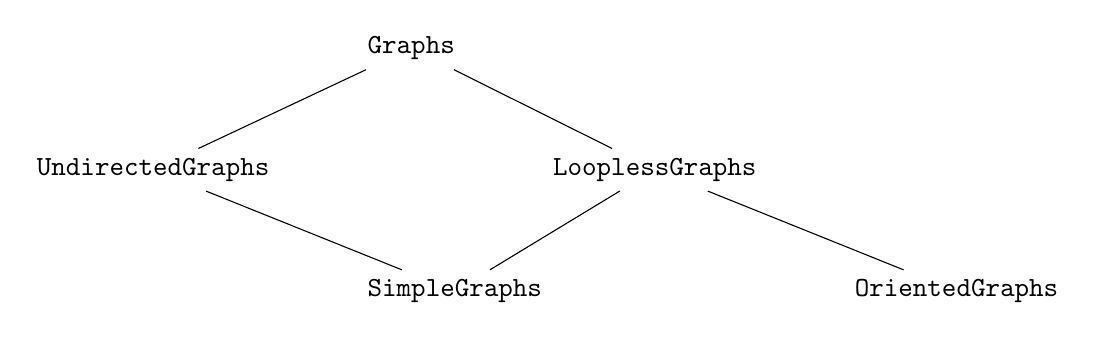
\begin{tikzpicture}[category/.style={font=\ttfamily}] \node (UG) [category]
{UndirectedGraphs}; \node (G) [category, above right=of UG] {Graphs}; \node
(SG) [category, below right=of UG] {SimpleGraphs}; \node (LG) [category, below
right=of G] {LooplessGraphs}; \node (OG) [category, below right=of LG]
{OrientedGraphs}; \draw (UG) -- (G) -- (LG) -- (OG); \draw (UG) -- (SG) --
(LG); \end{tikzpicture}   

 
\begin{Verbatim}[commandchars=!@|,fontsize=\small,frame=single,label=Example]
  !gapprompt@gap>| !gapinput@g1:=CompleteGraph(2:GraphCategory:=SimpleGraphs);  |
  Graph( Category := SimpleGraphs, Order := 2, Size := 
  1, Adjacencies := [ [ 2 ], [ 1 ] ] )
  !gapprompt@gap>| !gapinput@g2:=CompleteGraph(2:GraphCategory:=OrientedGraphs);|
  Graph( Category := OrientedGraphs, Order := 2, Size := 
  1, Adjacencies := [ [ 2 ], [  ] ] )
  !gapprompt@gap>| !gapinput@g3:=CompleteGraph(2:GraphCategory:=UndirectedGraphs);|
  Graph( Category := UndirectedGraphs, Order := 2, Size := 
  3, Adjacencies := [ [ 1, 2 ], [ 1, 2 ] ] )
  !gapprompt@gap>| !gapinput@GraphCategory([g1,g2,g3]);|
  <Category "Graphs">
  !gapprompt@gap>| !gapinput@GraphCategory([g1,g2]);   |
  <Category "LooplessGraphs">
  !gapprompt@gap>| !gapinput@GraphCategory([g1,g3]);|
  <Category "UndirectedGraphs">
\end{Verbatim}
 }

 

\subsection{\textcolor{Chapter }{Graphs}}
\logpage{[ "B", 7, 13 ]}\nobreak
\hyperdef{L}{X815691877F8C800C}{}
{\noindent\textcolor{FuncColor}{$\triangleright$\ \ \texttt{Graphs({\mdseries\slshape G})\index{Graphs@\texttt{Graphs}}
\label{Graphs}
}\hfill{\scriptsize (function)}}\\


 \texttt{Graphs} is the most general graph category in \textsf{YAGS}. This category contains all graphs that can be represented in \textsf{YAGS}. A graph in this category may contain loops, arrows and edges (which in \textsf{YAGS} are exactly the same as two opposite arrows between some pair of vertices).
This graph category has no parent category. \index{graphs} 

 
\begin{Verbatim}[commandchars=!@|,fontsize=\small,frame=single,label=Example]
  !gapprompt@gap>| !gapinput@GraphByWalks([1,1],[1,2],[2,1],[3,2]:GraphCategory:=Graphs);|
  Graph( Category := Graphs, Order := 3, Size := 4, Adjacencies := 
  [ [ 1, 2 ], [ 1 ], [ 2 ] ] )
  !gapprompt@gap>| !gapinput@GraphByWalks([1,1],[1,2],[2,1],[3,2]:GraphCategory:=SimpleGraphs);  |
  Graph( Category := SimpleGraphs, Order := 3, Size := 
  2, Adjacencies := [ [ 2 ], [ 1, 3 ], [ 2 ] ] )
\end{Verbatim}
 }

 

\subsection{\textcolor{Chapter }{GraphsOfGivenOrder}}
\logpage{[ "B", 7, 14 ]}\nobreak
\hyperdef{L}{X7F66DFB17CC3B2D9}{}
{\noindent\textcolor{FuncColor}{$\triangleright$\ \ \texttt{GraphsOfGivenOrder({\mdseries\slshape n})\index{GraphsOfGivenOrder@\texttt{GraphsOfGivenOrder}}
\label{GraphsOfGivenOrder}
}\hfill{\scriptsize (operation)}}\\


 

Returns the list of all graphs of order \mbox{\texttt{\mdseries\slshape n}} (up to isomorphism). This operation uses Brendan McKay's data published here: 

\href{https://cs.anu.edu.au/people/Brendan.McKay/data/graphs.html} {\texttt{https://cs.anu.edu.au/people/Brendan.McKay/data/graphs.html}}. 

These data are included with the \textsf{YAGS} distribution in its \texttt{data} directory. Hence this operation simply reads the corresponding file in that
directory using \texttt{ImportGraph6( \mbox{\texttt{\mdseries\slshape Filename}} )}. Therefore, the integer \mbox{\texttt{\mdseries\slshape n}} must be in the range from 1 up to 9. 


\begin{Verbatim}[commandchars=!@|,fontsize=\small,frame=single,label=Example]
  !gapprompt@gap>| !gapinput@GraphsOfGivenOrder(2);          |
  [ Graph( Category := SimpleGraphs, Order := 2, Size := 
      0, Adjacencies := [ [  ], [  ] ] ), 
    Graph( Category := SimpleGraphs, Order := 2, Size := 
      1, Adjacencies := [ [ 2 ], [ 1 ] ] ) ]
  !gapprompt@gap>| !gapinput@GraphsOfGivenOrder(3);|
  [ Graph( Category := SimpleGraphs, Order := 3, Size := 
      0, Adjacencies := [ [  ], [  ], [  ] ] ), 
    Graph( Category := SimpleGraphs, Order := 3, Size := 
      1, Adjacencies := [ [ 3 ], [  ], [ 1 ] ] ), 
    Graph( Category := SimpleGraphs, Order := 3, Size := 
      2, Adjacencies := [ [ 3 ], [ 3 ], [ 1, 2 ] ] ), 
    Graph( Category := SimpleGraphs, Order := 3, Size := 
      3, Adjacencies := [ [ 2, 3 ], [ 1, 3 ], [ 1, 2 ] ] ) ]
  !gapprompt@gap>| !gapinput@Length(GraphsOfGivenOrder(9));|
  274668
\end{Verbatim}
 

Data for graphs on 10 vertices is also available, but not included with \textsf{YAGS}, it may not be practical to use that data, but if you would like to try, all
you have to do is to copy (and to uncompress) the corresponding file into the
directory \texttt{YAGS-DIR/data/}. 

 
\begin{Verbatim}[commandchars=!@|,fontsize=\small,frame=single,label=Example]
  !gapprompt@gap>| !gapinput@GraphsOfGivenOrder(10);       |
  #W Unreadable File: /opt/gap4r8/pkg/yags/data/graph10.g6
  fail
\end{Verbatim}
 }

 

\subsection{\textcolor{Chapter }{GraphSum}}
\logpage{[ "B", 7, 15 ]}\nobreak
\hyperdef{L}{X7E8B61AD787C430F}{}
{\noindent\textcolor{FuncColor}{$\triangleright$\ \ \texttt{GraphSum({\mdseries\slshape G, L})\index{GraphSum@\texttt{GraphSum}}
\label{GraphSum}
}\hfill{\scriptsize (operation)}}\\


 

Returns the lexicographic sum of a list of graphs \mbox{\texttt{\mdseries\slshape L}} over a graph \mbox{\texttt{\mdseries\slshape G}}. 

The lexicographic sum is computed as follows: 

Given \mbox{\texttt{\mdseries\slshape G}}, with $Order( \mbox{\texttt{\mdseries\slshape G}} )=n$ and a list of $n$ graphs $\mbox{\texttt{\mdseries\slshape L}} = [G_1, \ldots, G_n]$, we take the disjoint union of $G_1,G_2, \ldots,G_n$ and then we add all the edges between $G_i$ and $G_j$ whenever $[i,j]$ is and edge of \mbox{\texttt{\mdseries\slshape G}}. 

If \mbox{\texttt{\mdseries\slshape L}} contains holes, the trivial graph is used in place. 


\begin{Verbatim}[commandchars=!@|,fontsize=\small,frame=single,label=Example]
  !gapprompt@gap>| !gapinput@t:=TrivialGraph;; g:=CycleGraph(4);;|
  !gapprompt@gap>| !gapinput@GraphSum(PathGraph(3),[t,g,t]);|
  Graph( Category := SimpleGraphs, Order := 6, Size := 
  12, Adjacencies := [ [ 2, 3, 4, 5 ], [ 1, 3, 5, 6 ], [ 1, 2, 4, 6 ], 
    [ 1, 3, 5, 6 ], [ 1, 2, 4, 6 ], [ 2, 3, 4, 5 ] ] )
  !gapprompt@gap>| !gapinput@GraphSum(PathGraph(3),[,g,]);  |
  Graph( Category := SimpleGraphs, Order := 6, Size := 
  12, Adjacencies := [ [ 2, 3, 4, 5 ], [ 1, 3, 5, 6 ], [ 1, 2, 4, 6 ], 
    [ 1, 3, 5, 6 ], [ 1, 2, 4, 6 ], [ 2, 3, 4, 5 ] ] )
\end{Verbatim}
 }

 

\subsection{\textcolor{Chapter }{GraphToRaw}}
\logpage{[ "B", 7, 16 ]}\nobreak
\hyperdef{L}{X8661587880C12114}{}
{\noindent\textcolor{FuncColor}{$\triangleright$\ \ \texttt{GraphToRaw({\mdseries\slshape FileName, G})\index{GraphToRaw@\texttt{GraphToRaw}}
\label{GraphToRaw}
}\hfill{\scriptsize (operation)}}\\


 

Converts a \textsf{YAGS} graph \mbox{\texttt{\mdseries\slshape G}} into a raw format (number of vertices, coordinates and adjacency matrix) and
writes the converted data to the file \mbox{\texttt{\mdseries\slshape FileName}}. For use by the external program \texttt{draw} (see \texttt{Draw} (\ref{Draw}) ). Intended for internal use only. 


\begin{Verbatim}[commandchars=!@|,fontsize=\small,frame=single,label=Example]
  !gapprompt@gap>| !gapinput@g:=CycleGraph(4);;|
  !gapprompt@gap>| !gapinput@GraphToRaw("mygraph.raw",g);|
\end{Verbatim}
 }

 

\subsection{\textcolor{Chapter }{GraphUpdateFromRaw}}
\logpage{[ "B", 7, 17 ]}\nobreak
\hyperdef{L}{X793E67DD83402749}{}
{\noindent\textcolor{FuncColor}{$\triangleright$\ \ \texttt{GraphUpdateFromRaw({\mdseries\slshape FileName, G})\index{GraphUpdateFromRaw@\texttt{GraphUpdateFromRaw}}
\label{GraphUpdateFromRaw}
}\hfill{\scriptsize (operation)}}\\


 

Updates the coordinates of \mbox{\texttt{\mdseries\slshape G}} from a file \mbox{\texttt{\mdseries\slshape FileName}} in raw format as written by \texttt{draw} (see \texttt{Draw} (\ref{Draw}) ). Intended for internal use only. }

 

\subsection{\textcolor{Chapter }{GroupGraph}}
\logpage{[ "B", 7, 18 ]}\nobreak
\hyperdef{L}{X78BA06B387DA3279}{}
{\noindent\textcolor{FuncColor}{$\triangleright$\ \ \texttt{GroupGraph({\mdseries\slshape G, Grp, Act})\index{GroupGraph@\texttt{GroupGraph}}
\label{GroupGraph}
}\hfill{\scriptsize (operation)}}\\
\noindent\textcolor{FuncColor}{$\triangleright$\ \ \texttt{GroupGraph({\mdseries\slshape G, Grp})\index{GroupGraph@\texttt{GroupGraph}}
\label{GroupGraph}
}\hfill{\scriptsize (operation)}}\\


 

Given a graph \mbox{\texttt{\mdseries\slshape G}}, a group \mbox{\texttt{\mdseries\slshape Grp}} and an action \mbox{\texttt{\mdseries\slshape Act}} of \mbox{\texttt{\mdseries\slshape Grp}} on some set S which contains $Vertices( \mbox{\texttt{\mdseries\slshape G}} )$, \texttt{GroupGraph} returns a new graph with vertex set $\{\mbox{\texttt{\mdseries\slshape Act}}(v,g) : g \in \mbox{\texttt{\mdseries\slshape Grp}}, v \in Vertices( \mbox{\texttt{\mdseries\slshape G}} )\}$ and edge set $\{\{\mbox{\texttt{\mdseries\slshape Act}}(v,g),\mbox{\texttt{\mdseries\slshape Act}}(u,g)\}: g\in \mbox{\texttt{\mdseries\slshape Grp}}, \{u,v\}\in Edges( \mbox{\texttt{\mdseries\slshape G}} )\}$. \index{graph!group} 

If \mbox{\texttt{\mdseries\slshape Act}} is omitted, the standard \textsf{GAP} action \texttt{OnPoints} is used. 


\begin{Verbatim}[commandchars=!@|,fontsize=\small,frame=single,label=Example]
  !gapprompt@gap>| !gapinput@GroupGraph(GraphByWalks([1,2]),Group([(1,2,3,4,5),(2,5)(3,4)]));|
  Graph( Category := SimpleGraphs, Order := 5, Size := 
  5, Adjacencies := [ [ 2, 5 ], [ 1, 3 ], [ 2, 4 ], [ 3, 5 ], [ 1, 4 ] 
   ] )
\end{Verbatim}
 }

 }

 
\section{\textcolor{Chapter }{H}}\label{H}
\logpage{[ "B", 8, 0 ]}
\hyperdef{L}{X81DA524381DA5243}{}
{
  

\subsection{\textcolor{Chapter }{HararyToMcKay}}
\logpage{[ "B", 8, 1 ]}\nobreak
\hyperdef{L}{X82276E097B77591E}{}
{\noindent\textcolor{FuncColor}{$\triangleright$\ \ \texttt{HararyToMcKay({\mdseries\slshape Spec})\index{HararyToMcKay@\texttt{HararyToMcKay}}
\label{HararyToMcKay}
}\hfill{\scriptsize (operation)}}\\
\noindent\textcolor{FuncColor}{$\triangleright$\ \ \texttt{McKayToHarary({\mdseries\slshape index})\index{McKayToHarary@\texttt{McKayToHarary}}
\label{McKayToHarary}
}\hfill{\scriptsize (operation)}}\\


 

Returns the McKay's \mbox{\texttt{\mdseries\slshape index}} of a Harary's graph specification \mbox{\texttt{\mdseries\slshape Spec}} and vice versa. Frank Harary published in his book \cite{Har69}, a list of all 208 simple graphs of order up to 6 (up to isomorphism). Each
of them had a label (which we call \mbox{\texttt{\mdseries\slshape Harary's graph specification}}) of the form \texttt{[ \mbox{\texttt{\mdseries\slshape n}}, \mbox{\texttt{\mdseries\slshape m}}, \mbox{\texttt{\mdseries\slshape s}} ]} where \mbox{\texttt{\mdseries\slshape n}} is the number of vertices, \mbox{\texttt{\mdseries\slshape m}} is the number of edges, and \mbox{\texttt{\mdseries\slshape s}} is a consecutive integer which uniquely identifies the graph from the others
with the same \mbox{\texttt{\mdseries\slshape n}} and \mbox{\texttt{\mdseries\slshape m}}. On the other hand, Brendan McKay published data sets containing a list of
all graphs of order up to 10 (also up to isomorphism), here: 

\href{https://cs.anu.edu.au/people/Brendan.McKay/data/graphs.html} {\texttt{https://cs.anu.edu.au/people/Brendan.McKay/data/graphs.html}} 

Each graph in these data sets appears in some specific position (which we call \emph{McKay's index}). We found it convenient to have an automated way to convert from Harary's
graph specifications to McKay's indexes and vice versa. 


\begin{Verbatim}[commandchars=!@|,fontsize=\small,frame=single,label=Example]
  !gapprompt@gap>| !gapinput@HararyToMcKay([1,0,1]); |
  1
  !gapprompt@gap>| !gapinput@HararyToMcKay([1,0,2]);|
  fail
  !gapprompt@gap>| !gapinput@HararyToMcKay([5,5,2]);|
  31
  !gapprompt@gap>| !gapinput@HararyToMcKay([5,5,3]);|
  34
  !gapprompt@gap>| !gapinput@HararyToMcKay([5,5,5]);|
  30
  !gapprompt@gap>| !gapinput@HararyToMcKay([5,5,6]);|
  45
  !gapprompt@gap>| !gapinput@HararyToMcKay([5,5,7]); |
  fail
  !gapprompt@gap>| !gapinput@HararyToMcKay([6,15,1]);|
  208
  !gapprompt@gap>| !gapinput@HararyToMcKay([6,15,2]);|
  fail
\end{Verbatim}
 


\begin{Verbatim}[commandchars=!@|,fontsize=\small,frame=single,label=Example]
  !gapprompt@gap>| !gapinput@List([1..208],McKayToHarary);|
  [ [ 1, 0, 1 ], [ 2, 0, 1 ], [ 2, 1, 1 ], [ 3, 0, 1 ], [ 3, 1, 1 ], 
    [ 3, 2, 1 ], [ 3, 3, 1 ], [ 4, 0, 1 ], [ 4, 1, 1 ], [ 4, 2, 1 ], 
    [ 4, 3, 3 ], [ 4, 2, 2 ], [ 4, 3, 1 ], [ 4, 3, 2 ], [ 4, 4, 1 ], 
  
                 --- many more lines here ---   
  
    [ 6, 10, 10 ], [ 6, 10, 7 ], [ 6, 11, 3 ], [ 6, 12, 1 ], [ 6, 13, 1 ], 
    [ 6, 11, 7 ], [ 6, 11, 9 ], [ 6, 11, 8 ], [ 6, 12, 4 ], [ 6, 12, 5 ], 
    [ 6, 13, 2 ], [ 6, 14, 1 ], [ 6, 15, 1 ] ]
  !gapprompt@gap>| !gapinput@McKayToHarary(209);|
  fail
\end{Verbatim}
 }

 

\subsection{\textcolor{Chapter }{HouseGraph}}
\logpage{[ "B", 8, 2 ]}\nobreak
\hyperdef{L}{X7FA941E678EAA379}{}
{\noindent\textcolor{FuncColor}{$\triangleright$\ \ \texttt{HouseGraph\index{HouseGraph@\texttt{HouseGraph}}
\label{HouseGraph}
}\hfill{\scriptsize (global variable)}}\\


 

A 4-cycle and a triangle glued by an edge. \index{graph!house} 

 
\begin{Verbatim}[commandchars=!@|,fontsize=\small,frame=single,label=Example]
  !gapprompt@gap>| !gapinput@HouseGraph;|
  Graph( Category := SimpleGraphs, Order := 5, Size := 
  6, Adjacencies := [ [ 2, 4, 5 ], [ 1, 3 ], [ 2, 4 ], [ 1, 3, 5 ], 
    [ 1, 4 ] ] )
\end{Verbatim}
 }

 }

 
\section{\textcolor{Chapter }{I}}\label{I}
\logpage{[ "B", 9, 0 ]}
\hyperdef{L}{X86AA214A86AA214A}{}
{
  

\subsection{\textcolor{Chapter }{Icosahedron}}
\logpage{[ "B", 9, 1 ]}\nobreak
\hyperdef{L}{X83E0EF8F7CCD6979}{}
{\noindent\textcolor{FuncColor}{$\triangleright$\ \ \texttt{Icosahedron\index{Icosahedron@\texttt{Icosahedron}}
\label{Icosahedron}
}\hfill{\scriptsize (global variable)}}\\


 

The 1-skeleton of Plato's icosahedron. 

 
\begin{Verbatim}[commandchars=!@|,fontsize=\small,frame=single,label=Example]
  !gapprompt@gap>| !gapinput@Icosahedron;|
  Graph( Category := SimpleGraphs, Order := 12, Size := 
  30, Adjacencies := [ [ 2, 3, 4, 5, 6 ], [ 1, 3, 6, 9, 10 ], 
    [ 1, 2, 4, 10, 11 ], [ 1, 3, 5, 7, 11 ], [ 1, 4, 6, 7, 8 ], 
    [ 1, 2, 5, 8, 9 ], [ 4, 5, 8, 11, 12 ], [ 5, 6, 7, 9, 12 ], 
    [ 2, 6, 8, 10, 12 ], [ 2, 3, 9, 11, 12 ], [ 3, 4, 7, 10, 12 ], 
    [ 7, 8, 9, 10, 11 ] ] )
\end{Verbatim}
 }

 

\subsection{\textcolor{Chapter }{ImportGraph6}}
\logpage{[ "B", 9, 2 ]}\nobreak
\hyperdef{L}{X7DF0F8C079D7D07D}{}
{\noindent\textcolor{FuncColor}{$\triangleright$\ \ \texttt{ImportGraph6({\mdseries\slshape Filename})\index{ImportGraph6@\texttt{ImportGraph6}}
\label{ImportGraph6}
}\hfill{\scriptsize (operation)}}\\


 

Returns the list of graphs represented in \mbox{\texttt{\mdseries\slshape Filename}} which are encoded using Brendan McKay's graph6 format. This operation allows
us to read data in databases which use this format. Several such databases can
be found here: \index{graph!importing from graph6 format} 

\href{https://cs.anu.edu.au/people/Brendan.McKay/data/graphs.html} {\texttt{https://cs.anu.edu.au/people/Brendan.McKay/data/graphs.html}}. 

The graph6 format is described here: 

\href{https://cs.anu.edu.au/people/Brendan.McKay/data/formats.txt} {\texttt{https://cs.anu.edu.au/people/Brendan.McKay/data/formats.txt}}. 

The following example assumes that you have a file named \texttt{graph3.g6} in your working directory which encodes graphs in graph6 format; the contents
of this file is assumed to be as indicated after the first command in the
example. It is also assumed that your Operative System is a Unix-like system. 


\begin{Verbatim}[commandchars=!@|,fontsize=\small,frame=single,label=Example]
  !gapprompt@gap>| !gapinput@Exec("cat graph3.g6");|
  B?
  BO
  BW
  Bw
  !gapprompt@gap>| !gapinput@ImportGraph6("graph3.g6");|
  [ Graph( Category := SimpleGraphs, Order := 3, Size := 0, Adjacencies := 
      [ [  ], [  ], [  ] ] ), Graph( Category := SimpleGraphs, Order := 
      3, Size := 1, Adjacencies := [ [ 3 ], [  ], [ 1 ] ] ), 
    Graph( Category := SimpleGraphs, Order := 3, Size := 2, Adjacencies := 
      [ [ 3 ], [ 3 ], [ 1, 2 ] ] ), Graph( Category := SimpleGraphs, Order :=
     3, Size := 3, Adjacencies := [ [ 2, 3 ], [ 1, 3 ], [ 1, 2 ] ] ) ]
\end{Verbatim}
 

See also \texttt{Graph6ToGraph} (\ref{Graph6ToGraph}). }

 

\subsection{\textcolor{Chapter }{in}}
\logpage{[ "B", 9, 3 ]}\nobreak
\hyperdef{L}{X87BDB89B7AAFE8AD}{}
{\noindent\textcolor{FuncColor}{$\triangleright$\ \ \texttt{in({\mdseries\slshape G, Catgy})\index{in@\texttt{in}}
\label{in}
}\hfill{\scriptsize (operation)}}\\


 

Returns \texttt{true} if graph \mbox{\texttt{\mdseries\slshape G}} belongs to category \mbox{\texttt{\mdseries\slshape Catgy}} and \texttt{false} otherwise. 

 
\begin{Verbatim}[commandchars=!@|,fontsize=\small,frame=single,label=Example]
  !gapprompt@gap>| !gapinput@g:=WheelGraph(4);|
  Graph( Category := SimpleGraphs, Order := 5, Size := 
  8, Adjacencies := [ [ 2, 3, 4, 5 ], [ 1, 3, 5 ], [ 1, 2, 4 ], 
    [ 1, 3, 5 ], [ 1, 2, 4 ] ] )
  !gapprompt@gap>| !gapinput@g in SimpleGraphs;|
  true
  !gapprompt@gap>| !gapinput@g in Graphs;|
  true
  !gapprompt@gap>| !gapinput@g in OrientedGraphs;|
  false
\end{Verbatim}
 }

 

\subsection{\textcolor{Chapter }{InducedSubgraph}}
\logpage{[ "B", 9, 4 ]}\nobreak
\hyperdef{L}{X7D9F576185C58545}{}
{\noindent\textcolor{FuncColor}{$\triangleright$\ \ \texttt{InducedSubgraph({\mdseries\slshape G, V})\index{InducedSubgraph@\texttt{InducedSubgraph}}
\label{InducedSubgraph}
}\hfill{\scriptsize (operation)}}\\


 

Returns the subgraph of the graph \mbox{\texttt{\mdseries\slshape G}} induced by the vertex set \mbox{\texttt{\mdseries\slshape V}}. \index{subgraph!induced} 

 
\begin{Verbatim}[commandchars=!@|,fontsize=\small,frame=single,label=Example]
  !gapprompt@gap>| !gapinput@g:=CycleGraph(6);          |
  Graph( Category := SimpleGraphs, Order := 6, Size := 
  6, Adjacencies := [ [ 2, 6 ], [ 1, 3 ], [ 2, 4 ], [ 3, 5 ], [ 4, 6 ], 
    [ 1, 5 ] ] )
  !gapprompt@gap>| !gapinput@InducedSubgraph(g,[3,4,6]);  |
  Graph( Category := SimpleGraphs, Order := 3, Size := 
  1, Adjacencies := [ [ 2 ], [ 1 ], [  ] ] )
\end{Verbatim}
 

The order of the elements in \mbox{\texttt{\mdseries\slshape V}} does matter. 

 
\begin{Verbatim}[commandchars=!@|,fontsize=\small,frame=single,label=Example]
  !gapprompt@gap>| !gapinput@InducedSubgraph(g,[6,3,4]);  |
  Graph( Category := SimpleGraphs, Order := 3, Size := 
  1, Adjacencies := [ [  ], [ 3 ], [ 2 ] ] )
\end{Verbatim}
 }

 

\subsection{\textcolor{Chapter }{InNeigh}}
\logpage{[ "B", 9, 5 ]}\nobreak
\hyperdef{L}{X78318B95813CAA26}{}
{\noindent\textcolor{FuncColor}{$\triangleright$\ \ \texttt{InNeigh({\mdseries\slshape G, x})\index{InNeigh@\texttt{InNeigh}}
\label{InNeigh}
}\hfill{\scriptsize (operation)}}\\


 

Returns the list of in-neighbors of \mbox{\texttt{\mdseries\slshape x}} in \mbox{\texttt{\mdseries\slshape G}}. 


\begin{Verbatim}[commandchars=!@|,fontsize=\small,frame=single,label=Example]
  !gapprompt@gap>| !gapinput@tt:=CompleteGraph(5:GraphCategory:=OrientedGraphs);|
  Graph( Category := OrientedGraphs, Order := 5, Size := 
  10, Adjacencies := [ [ 2, 3, 4, 5 ], [ 3, 4, 5 ], [ 4, 5 ], [ 5 ], 
    [  ] ] )
  !gapprompt@gap>| !gapinput@InNeigh(tt,3);                                     |
  [ 1, 2 ]
  !gapprompt@gap>| !gapinput@OutNeigh(tt,3);                                    |
  [ 4, 5 ]
\end{Verbatim}
 }

 

\subsection{\textcolor{Chapter }{InteriorVertices}}
\logpage{[ "B", 9, 6 ]}\nobreak
\hyperdef{L}{X7F43E2F0802FD790}{}
{\noindent\textcolor{FuncColor}{$\triangleright$\ \ \texttt{InteriorVertices({\mdseries\slshape G})\index{InteriorVertices@\texttt{InteriorVertices}}
\label{InteriorVertices}
}\hfill{\scriptsize (attribute)}}\\


 

When \mbox{\texttt{\mdseries\slshape G}} is a compact surface, it returns the list of vertices in the interior (of the
triangulation) of the surface. That is, the list of vertices of \mbox{\texttt{\mdseries\slshape G}} that have links isomorphic to a cycle. It returns \texttt{fail} if \mbox{\texttt{\mdseries\slshape G}} is not a compact surface. 


\begin{Verbatim}[commandchars=!@|,fontsize=\small,frame=single,label=Example]
  !gapprompt@gap>| !gapinput@InteriorVertices(WheelGraph(4,2));|
  [ 1, 2, 3, 4, 5 ]
  !gapprompt@gap>| !gapinput@InteriorVertices(Octahedron);     |
  [ 1, 2, 3, 4, 5, 6 ]
\end{Verbatim}
 }

 

\subsection{\textcolor{Chapter }{IntersectionGraph}}
\logpage{[ "B", 9, 7 ]}\nobreak
\hyperdef{L}{X827067C078A10B24}{}
{\noindent\textcolor{FuncColor}{$\triangleright$\ \ \texttt{IntersectionGraph({\mdseries\slshape L})\index{IntersectionGraph@\texttt{IntersectionGraph}}
\label{IntersectionGraph}
}\hfill{\scriptsize (function)}}\\


 

Returns the intersection graph of the family of sets \mbox{\texttt{\mdseries\slshape L}}. This graph has a vertex for every set in \mbox{\texttt{\mdseries\slshape L}}, and two such vertices are adjacent iff the corresponding sets have non-empty
intersection. \index{graph!intersection} 

 
\begin{Verbatim}[commandchars=!@|,fontsize=\small,frame=single,label=Example]
  !gapprompt@gap>| !gapinput@IntersectionGraph([[1,2,3],[3,4,5],[5,6,7]]);|
  Graph( Category := SimpleGraphs, Order := 3, Size := 
  2, Adjacencies := [ [ 2 ], [ 1, 3 ], [ 2 ] ] )
\end{Verbatim}
 }

 

\subsection{\textcolor{Chapter }{IsBoolean}}
\logpage{[ "B", 9, 8 ]}\nobreak
\hyperdef{L}{X80FF64FC7E750046}{}
{\noindent\textcolor{FuncColor}{$\triangleright$\ \ \texttt{IsBoolean({\mdseries\slshape Obj})\index{IsBoolean@\texttt{IsBoolean}}
\label{IsBoolean}
}\hfill{\scriptsize (function)}}\\


 

Returns \texttt{true} if object \mbox{\texttt{\mdseries\slshape Obj}} is \texttt{true} or \texttt{false} and \texttt{false} otherwise. 

 
\begin{Verbatim}[commandchars=!@|,fontsize=\small,frame=single,label=Example]
  !gapprompt@gap>| !gapinput@IsBoolean( true ); IsBoolean( fail ); IsBoolean ( false );|
  true
  false
  true
\end{Verbatim}
 }

 

\subsection{\textcolor{Chapter }{IsCliqueGated}}
\logpage{[ "B", 9, 9 ]}\nobreak
\hyperdef{L}{X78F70A8B7C72464C}{}
{\noindent\textcolor{FuncColor}{$\triangleright$\ \ \texttt{IsCliqueGated({\mdseries\slshape G})\index{IsCliqueGated@\texttt{IsCliqueGated}}
\label{IsCliqueGated}
}\hfill{\scriptsize (property)}}\\


 

Returns \texttt{true} if \mbox{\texttt{\mdseries\slshape G}} is a clique gated graph \cite{HK96}. 

This operation reports progress at \texttt{InfoLevel} 1 (see \ref{YAGSInfo.InfoClass}). }

 

\subsection{\textcolor{Chapter }{IsCliqueHelly}}
\logpage{[ "B", 9, 10 ]}\nobreak
\hyperdef{L}{X822B38D686BC1D2D}{}
{\noindent\textcolor{FuncColor}{$\triangleright$\ \ \texttt{IsCliqueHelly({\mdseries\slshape G})\index{IsCliqueHelly@\texttt{IsCliqueHelly}}
\label{IsCliqueHelly}
}\hfill{\scriptsize (property)}}\\


 

Returns \texttt{true} if the set of (maximal) cliques \mbox{\texttt{\mdseries\slshape G}} satisfy the \emph{Helly} property. \index{clique-Helly} 

The Helly property is defined as follows: 

A non-empty family $F$ of non-empty sets satisfies the Helly property if every pairwise intersecting
subfamily of $F$ has a non-empty total intersection. \index{Helly property} 

Here we use the Dragan-Szwarcfiter characterization \cite{Dra89}\cite{Szw97} to compute the Helly property. \index{clique-Helly!Dragan-Szwarcfiter characterization} 


\begin{Verbatim}[commandchars=!@|,fontsize=\small,frame=single,label=Example]
  !gapprompt@gap>| !gapinput@g:=SunGraph(3);|
  Graph( Category := SimpleGraphs, Order := 6, Size := 
  9, Adjacencies := [ [ 2, 6 ], [ 1, 3, 4, 6 ], [ 2, 4 ], 
    [ 2, 3, 5, 6 ], [ 4, 6 ], [ 1, 2, 4, 5 ] ] )
  !gapprompt@gap>| !gapinput@IsCliqueHelly(g);|
  false
\end{Verbatim}
 }

 

\subsection{\textcolor{Chapter }{IsCompactSurface}}
\logpage{[ "B", 9, 11 ]}\nobreak
\hyperdef{L}{X8563061F83E10A23}{}
{\noindent\textcolor{FuncColor}{$\triangleright$\ \ \texttt{IsCompactSurface({\mdseries\slshape G})\index{IsCompactSurface@\texttt{IsCompactSurface}}
\label{IsCompactSurface}
}\hfill{\scriptsize (property)}}\\


 

Returns \texttt{true} if every link of \mbox{\texttt{\mdseries\slshape G}} is either an \mbox{\texttt{\mdseries\slshape n}}-cycle, for $n\geq 4$ or an \mbox{\texttt{\mdseries\slshape m}}-path, for $m\geq 2$. (not necessarily the same \mbox{\texttt{\mdseries\slshape n}}/\mbox{\texttt{\mdseries\slshape m}} for all vertices); it returns \texttt{false} otherwise. 

This notion correspond to Whitney triangulations of compact surfaces \cite{LNP02} in which the (maximal) cliques of the graph are exactly the triangles of the
triangulation. 


\begin{Verbatim}[commandchars=!@|,fontsize=\small,frame=single,label=Example]
  !gapprompt@gap>| !gapinput@IsCompactSurface(Icosahedron);                             |
  true
  !gapprompt@gap>| !gapinput@IsCompactSurface(RemoveVertices(Icosahedron,[1]));|
  true
  !gapprompt@gap>| !gapinput@IsCompactSurface(WheelGraph(4,2));|
  true
  !gapprompt@gap>| !gapinput@IsCompactSurface(Tetrahedron);    |
  false
  !gapprompt@gap>| !gapinput@IsCompactSurface(CompleteGraph(2));|
  false
  !gapprompt@gap>| !gapinput@IsCompactSurface(CompleteGraph(3));|
  true
  !gapprompt@gap>| !gapinput@IsCompactSurface(CompleteGraph(4));|
  false
\end{Verbatim}
 

Topologically, the difference between a surface and a compact surface is that
the points of a surface always have a open neighborhood homeomorphic to an
open disk, whereas a compact surface may also contain points with open
neighborhoods homeomorphic to a closed half-plane. }

 

\subsection{\textcolor{Chapter }{IsComplete}}
\logpage{[ "B", 9, 12 ]}\nobreak
\hyperdef{L}{X7D689F21828A4278}{}
{\noindent\textcolor{FuncColor}{$\triangleright$\ \ \texttt{IsComplete({\mdseries\slshape G, L})\index{IsComplete@\texttt{IsComplete}}
\label{IsComplete}
}\hfill{\scriptsize (operation)}}\\


 

Returns \texttt{true} if \mbox{\texttt{\mdseries\slshape L}} induces a complete subgraph of \mbox{\texttt{\mdseries\slshape G}}. 

 
\begin{Verbatim}[commandchars=!@|,fontsize=\small,frame=single,label=Example]
  !gapprompt@gap>| !gapinput@IsComplete(DiamondGraph,[1,2,3]);|
  true
  !gapprompt@gap>| !gapinput@IsComplete(DiamondGraph,[1,2,4]);|
  false
\end{Verbatim}
 }

 

\subsection{\textcolor{Chapter }{IsCompleteGraph}}
\logpage{[ "B", 9, 13 ]}\nobreak
\hyperdef{L}{X7BA6EF9F80968CD8}{}
{\noindent\textcolor{FuncColor}{$\triangleright$\ \ \texttt{IsCompleteGraph({\mdseries\slshape G})\index{IsCompleteGraph@\texttt{IsCompleteGraph}}
\label{IsCompleteGraph}
}\hfill{\scriptsize (property)}}\\


 

Returns \texttt{true} if graph \mbox{\texttt{\mdseries\slshape G}} is a complete graph, \texttt{false} otherwise. In a complete graph every pair of vertices is an edge. }

 

\subsection{\textcolor{Chapter }{IsDiamondFree}}
\logpage{[ "B", 9, 14 ]}\nobreak
\hyperdef{L}{X7D03ACD07C167E0F}{}
{\noindent\textcolor{FuncColor}{$\triangleright$\ \ \texttt{IsDiamondFree({\mdseries\slshape G})\index{IsDiamondFree@\texttt{IsDiamondFree}}
\label{IsDiamondFree}
}\hfill{\scriptsize (property)}}\\


 

Returns \texttt{true} if \mbox{\texttt{\mdseries\slshape G}} is free from induced diamonds (see \texttt{DiamondGraph} (\ref{DiamondGraph})); \texttt{false} otherwise. 


\begin{Verbatim}[commandchars=!@|,fontsize=\small,frame=single,label=Example]
  !gapprompt@gap>| !gapinput@IsDiamondFree(Cube);|
  true
  !gapprompt@gap>| !gapinput@IsDiamondFree(Octahedron);|
  false
\end{Verbatim}
 }

 

\subsection{\textcolor{Chapter }{IsEdge}}
\logpage{[ "B", 9, 15 ]}\nobreak
\hyperdef{L}{X7F50265D789C602C}{}
{\noindent\textcolor{FuncColor}{$\triangleright$\ \ \texttt{IsEdge({\mdseries\slshape G, x, y})\index{IsEdge@\texttt{IsEdge}}
\label{IsEdge}
}\hfill{\scriptsize (operation)}}\\
\noindent\textcolor{FuncColor}{$\triangleright$\ \ \texttt{IsEdge({\mdseries\slshape G, e})\index{IsEdge@\texttt{IsEdge}}
\label{IsEdge}
}\hfill{\scriptsize (operation)}}\\


 

Returns \texttt{true} if \texttt{e:=[\mbox{\texttt{\mdseries\slshape x}},\mbox{\texttt{\mdseries\slshape y}}]} is an edge of \mbox{\texttt{\mdseries\slshape G}}. 

 
\begin{Verbatim}[commandchars=!@|,fontsize=\small,frame=single,label=Example]
  !gapprompt@gap>| !gapinput@IsEdge(PathGraph(3),1,2);|
  true
  !gapprompt@gap>| !gapinput@IsEdge(PathGraph(3),[1,2]);|
  true
  !gapprompt@gap>| !gapinput@IsEdge(PathGraph(3),1,3);|
  false
  !gapprompt@gap>| !gapinput@IsEdge(PathGraph(3),[1,3]);|
  false
\end{Verbatim}
 

The first form, \texttt{IsEdge(\mbox{\texttt{\mdseries\slshape G}}, \mbox{\texttt{\mdseries\slshape x}}, \mbox{\texttt{\mdseries\slshape y}})}, is a bit faster and hence more suitable for use in algorithms which make
extensive use of this operation. On the other hand, the first form does no
error checking at all, and hence, it may produce an error where the second
form returns false (for instance when \mbox{\texttt{\mdseries\slshape x}} is not a vertex of \mbox{\texttt{\mdseries\slshape G}}). The second form is therefore a bit slower, but more robust. 

 
\begin{Verbatim}[commandchars=!@|,fontsize=\small,frame=single,label=Example]
  !gapprompt@gap>| !gapinput@IsEdge(PathGraph(3),[7,3]);|
  false
  !gapprompt@gap>| !gapinput@IsEdge(PathGraph(3),7,3);  |
  Error, List Element: <list>[7] must have an assigned value
\end{Verbatim}
 }

 

\subsection{\textcolor{Chapter }{IsIsomorphicGraph}}
\logpage{[ "B", 9, 16 ]}\nobreak
\hyperdef{L}{X79CBEA7386509498}{}
{\noindent\textcolor{FuncColor}{$\triangleright$\ \ \texttt{IsIsomorphicGraph({\mdseries\slshape G, H})\index{IsIsomorphicGraph@\texttt{IsIsomorphicGraph}}
\label{IsIsomorphicGraph}
}\hfill{\scriptsize (operation)}}\\


 

Returns \texttt{true} when \mbox{\texttt{\mdseries\slshape G}} is isomorphic to \mbox{\texttt{\mdseries\slshape H}} and \texttt{false} otherwise. \index{graphs!isomorphic} 


\begin{Verbatim}[commandchars=!@|,fontsize=\small,frame=single,label=Example]
  !gapprompt@gap>| !gapinput@g:=PowerGraph(CycleGraph(6),2);;h:=Octahedron;;|
  !gapprompt@gap>| !gapinput@IsIsomorphicGraph(g,h);|
  true
\end{Verbatim}
 }

 

\subsection{\textcolor{Chapter }{IsLocallyConstant}}
\logpage{[ "B", 9, 17 ]}\nobreak
\hyperdef{L}{X782871638792F4F5}{}
{\noindent\textcolor{FuncColor}{$\triangleright$\ \ \texttt{IsLocallyConstant({\mdseries\slshape G})\index{IsLocallyConstant@\texttt{IsLocallyConstant}}
\label{IsLocallyConstant}
}\hfill{\scriptsize (property)}}\\


 

Returns \texttt{true} if all the links of \mbox{\texttt{\mdseries\slshape G}} are isomorphic to each other; \texttt{false} otherwise. \index{locally constant} \index{graph!locally constant} 


\begin{Verbatim}[commandchars=!@|,fontsize=\small,frame=single,label=Example]
  !gapprompt@gap>| !gapinput@IsLocallyConstant(PathGraph(2));|
  true
  !gapprompt@gap>| !gapinput@IsLocallyConstant(PathGraph(3));|
  false
  !gapprompt@gap>| !gapinput@IsLocallyConstant(CompleteGraph(3));|
  true
  !gapprompt@gap>| !gapinput@IsLocallyConstant(CycleGraph(4));   |
  true
  !gapprompt@gap>| !gapinput@IsLocallyConstant(Icosahedron);  |
  true
  !gapprompt@gap>| !gapinput@IsLocallyConstant(TorusGraph(5,4));|
  true
  !gapprompt@gap>| !gapinput@IsLocallyConstant(WheelGraph(4,2));|
  false
  !gapprompt@gap>| !gapinput@IsLocallyConstant(SnubDisphenoid); |
  false
\end{Verbatim}
 }

 

\subsection{\textcolor{Chapter }{IsLocallyH}}
\logpage{[ "B", 9, 18 ]}\nobreak
\hyperdef{L}{X7ACED06884FBC782}{}
{\noindent\textcolor{FuncColor}{$\triangleright$\ \ \texttt{IsLocallyH({\mdseries\slshape G, H})\index{IsLocallyH@\texttt{IsLocallyH}}
\label{IsLocallyH}
}\hfill{\scriptsize (operation)}}\\


 

Returns \texttt{true} if all the links of \mbox{\texttt{\mdseries\slshape G}} are isomorphic to \mbox{\texttt{\mdseries\slshape H}}; \texttt{false} otherwise. \index{locally H} \index{graph!locally H} 


\begin{Verbatim}[commandchars=!@|,fontsize=\small,frame=single,label=Example]
  !gapprompt@gap>| !gapinput@IsLocallyH(Octahedron,CycleGraph(4));|
  true
  !gapprompt@gap>| !gapinput@IsLocallyH(Octahedron,CycleGraph(5));|
  false
  !gapprompt@gap>| !gapinput@IsLocallyH(Icosahedron,CycleGraph(5));|
  true
  !gapprompt@gap>| !gapinput@IsLocallyH(TorusGraph(4,4),CycleGraph(6));|
  true
\end{Verbatim}
 }

 

\subsection{\textcolor{Chapter }{IsLoopless}}
\logpage{[ "B", 9, 19 ]}\nobreak
\hyperdef{L}{X7F9F4622817E9AFB}{}
{\noindent\textcolor{FuncColor}{$\triangleright$\ \ \texttt{IsLoopless({\mdseries\slshape G})\index{IsLoopless@\texttt{IsLoopless}}
\label{IsLoopless}
}\hfill{\scriptsize (property)}}\\


 

Returns \texttt{true} if the graph \mbox{\texttt{\mdseries\slshape G}} have no loops; \texttt{false} otherwise. Loops are edges from a vertex to itself. }

 

\subsection{\textcolor{Chapter }{IsoMorphism}}
\logpage{[ "B", 9, 20 ]}\nobreak
\hyperdef{L}{X80F38E797C303471}{}
{\noindent\textcolor{FuncColor}{$\triangleright$\ \ \texttt{IsoMorphism({\mdseries\slshape G, H})\index{IsoMorphism@\texttt{IsoMorphism}}
\label{IsoMorphism}
}\hfill{\scriptsize (operation)}}\\


 

Returns one isomorphism from \mbox{\texttt{\mdseries\slshape G}} to \mbox{\texttt{\mdseries\slshape H}} or \texttt{fail} if none exists. If \mbox{\texttt{\mdseries\slshape G}} has \texttt{n} vertices, an isomorphisms $f : \mbox{\texttt{\mdseries\slshape G}}\rightarrow \mbox{\texttt{\mdseries\slshape H}}$ is represented as the list \texttt{\mbox{\texttt{\mdseries\slshape F}}=[f(1), f(2), ..., f(n)]}. 


\begin{Verbatim}[commandchars=!@|,fontsize=\small,frame=single,label=Example]
  !gapprompt@gap>| !gapinput@g:=CycleGraph(4);;h:=CompleteBipartiteGraph(2,2);;|
  !gapprompt@gap>| !gapinput@f:=IsoMorphism(g,h);|
  [ 1, 3, 2, 4 ]
\end{Verbatim}
 

See \texttt{NextIsoMorphism} (\ref{NextIsoMorphism}). }

 

\subsection{\textcolor{Chapter }{IsoMorphisms}}
\logpage{[ "B", 9, 21 ]}\nobreak
\hyperdef{L}{X7D702EA087C1C5EF}{}
{\noindent\textcolor{FuncColor}{$\triangleright$\ \ \texttt{IsoMorphisms({\mdseries\slshape G, H})\index{IsoMorphisms@\texttt{IsoMorphisms}}
\label{IsoMorphisms}
}\hfill{\scriptsize (operation)}}\\


 

Returns the list of all isomorphism from \mbox{\texttt{\mdseries\slshape G}} to \mbox{\texttt{\mdseries\slshape H}}. If \mbox{\texttt{\mdseries\slshape G}} has \texttt{n} vertices, an isomorphisms $f:\mbox{\texttt{\mdseries\slshape G}}\rightarrow \mbox{\texttt{\mdseries\slshape H}}$ is represented as the list \texttt{\mbox{\texttt{\mdseries\slshape F}}=[f(1), f(2), ..., f(n)]}. 


\begin{Verbatim}[commandchars=!@|,fontsize=\small,frame=single,label=Example]
  !gapprompt@gap>| !gapinput@g:=CycleGraph(4);;h:=CompleteBipartiteGraph(2,2);;|
  !gapprompt@gap>| !gapinput@IsoMorphisms(g,h);|
  [ [ 1, 3, 2, 4 ], [ 1, 4, 2, 3 ], [ 2, 3, 1, 4 ], [ 2, 4, 1, 3 ], 
    [ 3, 1, 4, 2 ], [ 3, 2, 4, 1 ], [ 4, 1, 3, 2 ], [ 4, 2, 3, 1 ] ]
\end{Verbatim}
 }

 

\subsection{\textcolor{Chapter }{IsOriented}}
\logpage{[ "B", 9, 22 ]}\nobreak
\hyperdef{L}{X8278D52F856A179D}{}
{\noindent\textcolor{FuncColor}{$\triangleright$\ \ \texttt{IsOriented({\mdseries\slshape G})\index{IsOriented@\texttt{IsOriented}}
\label{IsOriented}
}\hfill{\scriptsize (property)}}\\


 

Returns \texttt{true} if the graph \mbox{\texttt{\mdseries\slshape G}} is an oriented graph, \texttt{false} otherwise. Regardless of the categories that \mbox{\texttt{\mdseries\slshape G}} belongs to, \mbox{\texttt{\mdseries\slshape G}} is oriented if whenever \texttt{[x,y]} is an edge of \mbox{\texttt{\mdseries\slshape G}}, \texttt{[y,x]} is not. }

 

\subsection{\textcolor{Chapter }{IsSimple}}
\logpage{[ "B", 9, 23 ]}\nobreak
\hyperdef{L}{X7D8E63A7824037CC}{}
{\noindent\textcolor{FuncColor}{$\triangleright$\ \ \texttt{IsSimple({\mdseries\slshape G})\index{IsSimple@\texttt{IsSimple}}
\label{IsSimple}
}\hfill{\scriptsize (property)}}\\


 

Returns \texttt{true} if the graph \mbox{\texttt{\mdseries\slshape G}} is a simple graph, \texttt{false} otherwise. Regardless of the categories that \mbox{\texttt{\mdseries\slshape G}} belongs to, \mbox{\texttt{\mdseries\slshape G}} is simple if and only if \mbox{\texttt{\mdseries\slshape G}} is undirected and loopless. }

 

\subsection{\textcolor{Chapter }{IsSurface}}
\logpage{[ "B", 9, 24 ]}\nobreak
\hyperdef{L}{X8393259C7C8C4B73}{}
{\noindent\textcolor{FuncColor}{$\triangleright$\ \ \texttt{IsSurface({\mdseries\slshape G})\index{IsSurface@\texttt{IsSurface}}
\label{IsSurface}
}\hfill{\scriptsize (property)}}\\


 

Returns \texttt{true} if every link of \mbox{\texttt{\mdseries\slshape G}} is an \mbox{\texttt{\mdseries\slshape n}}-cycle, for $n\geq 4$ (not necessarily the same \mbox{\texttt{\mdseries\slshape n}} for all vertices); \texttt{false} otherwise. 

This notion correspond to Whitney triangulations of (closed) surfaces \cite{LNP02} in which the (maximal) cliques of the graph are exactly the triangles of the
triangulation. 


\begin{Verbatim}[commandchars=!@|,fontsize=\small,frame=single,label=Example]
  !gapprompt@gap>| !gapinput@IsSurface(SnubDisphenoid);|
  true
  !gapprompt@gap>| !gapinput@IsSurface(Icosahedron);   |
  true
  !gapprompt@gap>| !gapinput@IsSurface(RemoveVertices(Icosahedron,[1]));       |
  false
  !gapprompt@gap>| !gapinput@IsSurface(TorusGraph(4,5));|
  true
  !gapprompt@gap>| !gapinput@IsSurface(WheelGraph(4,2));|
  false
  !gapprompt@gap>| !gapinput@IsSurface(Tetrahedron);    |
  false
\end{Verbatim}
 

Topologically, the difference between a (closed) surface and a compact surface
is that the points of a surface always have a open neighborhood homeomorphic
to an open disk, whereas a compact surface may also contain points with open
neighborhoods homeomorphic to a closed half-plane. }

 

\subsection{\textcolor{Chapter }{IsTournament}}
\logpage{[ "B", 9, 25 ]}\nobreak
\hyperdef{L}{X7DD8D1A185EBE865}{}
{\noindent\textcolor{FuncColor}{$\triangleright$\ \ \texttt{IsTournament({\mdseries\slshape G})\index{IsTournament@\texttt{IsTournament}}
\label{IsTournament}
}\hfill{\scriptsize (property)}}\\


 

Returns \texttt{true} if \mbox{\texttt{\mdseries\slshape G}} is a tournament. A \emph{tournament} is a graph without loops and such that for every pair of vertices \texttt{x}, \texttt{y}, either \texttt{[x,y]} is an arrow of \mbox{\texttt{\mdseries\slshape G}} , or \texttt{[y,x]} is an arrow of \mbox{\texttt{\mdseries\slshape G}}, but not both. \index{tournament} 


\begin{Verbatim}[commandchars=!@|,fontsize=\small,frame=single,label=Example]
  !gapprompt@gap>| !gapinput@tt:=CompleteGraph(5:GraphCategory:=OrientedGraphs);|
  Graph( Category := OrientedGraphs, Order := 5, Size := 
  10, Adjacencies := [ [ 2, 3, 4, 5 ], [ 3, 4, 5 ], [ 4, 5 ], [ 5 ], 
    [  ] ] )
  !gapprompt@gap>| !gapinput@IsTournament(tt);                                  |
  true
\end{Verbatim}
 }

 

\subsection{\textcolor{Chapter }{IsTransitiveTournament}}
\logpage{[ "B", 9, 26 ]}\nobreak
\hyperdef{L}{X7CC7E10386094A61}{}
{\noindent\textcolor{FuncColor}{$\triangleright$\ \ \texttt{IsTransitiveTournament({\mdseries\slshape G})\index{IsTransitiveTournament@\texttt{IsTransitiveTournament}}
\label{IsTransitiveTournament}
}\hfill{\scriptsize (property)}}\\


 

Returns \texttt{true} if \mbox{\texttt{\mdseries\slshape G}} is a transitive tournament. A tournament is a \emph{transitive tournament} if whenever \texttt{[x,y]} and \texttt{[y,z]} are arrows of the tournament, \texttt{[x,z]} is also an arrow of the tournament. \index{tournament!transitive} \index{transitive tournament} 


\begin{Verbatim}[commandchars=!@|,fontsize=\small,frame=single,label=Example]
  !gapprompt@gap>| !gapinput@tt:=CompleteGraph(5:GraphCategory:=OrientedGraphs);|
  Graph( Category := OrientedGraphs, Order := 5, Size := 
  10, Adjacencies := [ [ 2, 3, 4, 5 ], [ 3, 4, 5 ], [ 4, 5 ], [ 5 ], 
    [  ] ] )
  !gapprompt@gap>| !gapinput@IsTransitiveTournament(tt);|
  true
\end{Verbatim}
 }

 

\subsection{\textcolor{Chapter }{IsUndirected}}
\logpage{[ "B", 9, 27 ]}\nobreak
\hyperdef{L}{X872108F17D8F264D}{}
{\noindent\textcolor{FuncColor}{$\triangleright$\ \ \texttt{IsUndirected({\mdseries\slshape G})\index{IsUndirected@\texttt{IsUndirected}}
\label{IsUndirected}
}\hfill{\scriptsize (property)}}\\


 

Returns \texttt{true} if the graph \mbox{\texttt{\mdseries\slshape G}} is an undirected graph; \texttt{false} otherwise. Regardless of the categories that \mbox{\texttt{\mdseries\slshape G}} belongs to, \mbox{\texttt{\mdseries\slshape G}} is undirected if whenever \texttt{[x,y]} is an edge of \mbox{\texttt{\mdseries\slshape G}}, \texttt{[y,x]} is also an edge of \mbox{\texttt{\mdseries\slshape G}}. }

 }

 
\section{\textcolor{Chapter }{J}}\label{J}
\logpage{[ "B", 10, 0 ]}
\hyperdef{L}{X7F3AB4517F3AB451}{}
{
  

\subsection{\textcolor{Chapter }{JohnsonGraph}}
\logpage{[ "B", 10, 1 ]}\nobreak
\hyperdef{L}{X7A4036667F52738C}{}
{\noindent\textcolor{FuncColor}{$\triangleright$\ \ \texttt{JohnsonGraph({\mdseries\slshape n, r})\index{JohnsonGraph@\texttt{JohnsonGraph}}
\label{JohnsonGraph}
}\hfill{\scriptsize (function)}}\\


 

Returns the \emph{Johnson graph} $J(n,r)$. The Johnson graph is the graph whose vertices are \mbox{\texttt{\mdseries\slshape r}}-subset of the set $\{1, 2, \ldots, n\}$, two of them being adjacent iff they intersect in exactly \texttt{\mbox{\texttt{\mdseries\slshape r}}-1} elements. \index{graph!Johnson} \index{Johnson graph} 

 
\begin{Verbatim}[commandchars=!@|,fontsize=\small,frame=single,label=Example]
  !gapprompt@gap>| !gapinput@g:=JohnsonGraph(4,2);                                            |
  Graph( Category := SimpleGraphs, Order := 6, Size := 
  12, Adjacencies := [ [ 2, 3, 4, 5 ], [ 1, 3, 4, 6 ], [ 1, 2, 5, 6 ], 
    [ 1, 2, 5, 6 ], [ 1, 3, 4, 6 ], [ 2, 3, 4, 5 ] ] )
  !gapprompt@gap>| !gapinput@VertexNames(g);|
  [ [ 1, 2 ], [ 1, 3 ], [ 1, 4 ], [ 2, 3 ], [ 2, 4 ], [ 3, 4 ] ]
\end{Verbatim}
 }

 

\subsection{\textcolor{Chapter }{Join}}
\logpage{[ "B", 10, 2 ]}\nobreak
\hyperdef{L}{X7870C5F085DD4D77}{}
{\noindent\textcolor{FuncColor}{$\triangleright$\ \ \texttt{Join({\mdseries\slshape G, H})\index{Join@\texttt{Join}}
\label{Join}
}\hfill{\scriptsize (operation)}}\\


 

Returns the join graph \mbox{\texttt{\mdseries\slshape G}} + \mbox{\texttt{\mdseries\slshape H}} of \mbox{\texttt{\mdseries\slshape G}} and \mbox{\texttt{\mdseries\slshape H}} (also known as the Zykov sum\index{Zykov sum}); it is the graph obtained from the disjoint union of \mbox{\texttt{\mdseries\slshape G}} and \mbox{\texttt{\mdseries\slshape H}} by adding every possible edge from every vertex in \mbox{\texttt{\mdseries\slshape G}} to every vertex in \mbox{\texttt{\mdseries\slshape H}}. 


\begin{Verbatim}[commandchars=!@|,fontsize=\small,frame=single,label=Example]
  !gapprompt@gap>| !gapinput@g:=DiscreteGraph(2);h:=CycleGraph(4);|
  Graph( Category := SimpleGraphs, Order := 2, Size := 
  0, Adjacencies := [ [  ], [  ] ] )
  Graph( Category := SimpleGraphs, Order := 4, Size := 
  4, Adjacencies := [ [ 2, 4 ], [ 1, 3 ], [ 2, 4 ], [ 1, 3 ] ] )
  !gapprompt@gap>| !gapinput@Join(g,h);                           |
  Graph( Category := SimpleGraphs, Order := 6, Size := 
  12, Adjacencies := [ [ 3, 4, 5, 6 ], [ 3, 4, 5, 6 ], [ 1, 2, 4, 6 ], 
    [ 1, 2, 3, 5 ], [ 1, 2, 4, 6 ], [ 1, 2, 3, 5 ] ] )
\end{Verbatim}
 }

 }

 
\section{\textcolor{Chapter }{K}}\label{K}
\logpage{[ "B", 11, 0 ]}
\hyperdef{L}{X784AC758784AC758}{}
{
  

\subsection{\textcolor{Chapter }{KiteGraph}}
\logpage{[ "B", 11, 1 ]}\nobreak
\hyperdef{L}{X854EB85A7F08DE43}{}
{\noindent\textcolor{FuncColor}{$\triangleright$\ \ \texttt{KiteGraph\index{KiteGraph@\texttt{KiteGraph}}
\label{KiteGraph}
}\hfill{\scriptsize (global variable)}}\\


 

A diamond (see \texttt{DiamondGraph} (\ref{DiamondGraph})) with a pendant vertex and maximum degree 3. \index{graph!kite} 

 
\begin{Verbatim}[commandchars=!@|,fontsize=\small,frame=single,label=Example]
  !gapprompt@gap>| !gapinput@KiteGraph;|
  Graph( Category := SimpleGraphs, Order := 5, Size := 
  6, Adjacencies := [ [ 2 ], [ 1, 3, 4 ], [ 2, 4, 5 ], [ 2, 3, 5 ], 
    [ 3, 4 ] ] )
\end{Verbatim}
 }

 }

 
\section{\textcolor{Chapter }{L}}\label{L}
\logpage{[ "B", 12, 0 ]}
\hyperdef{L}{X81AC8E0281AC8E02}{}
{
  

\subsection{\textcolor{Chapter }{LineGraph}}
\logpage{[ "B", 12, 1 ]}\nobreak
\hyperdef{L}{X7F3242BE87F58573}{}
{\noindent\textcolor{FuncColor}{$\triangleright$\ \ \texttt{LineGraph({\mdseries\slshape G})\index{LineGraph@\texttt{LineGraph}}
\label{LineGraph}
}\hfill{\scriptsize (operation)}}\\


 

Returns the \emph{line graph}, \mbox{\texttt{\mdseries\slshape L(G)}}, of graph \mbox{\texttt{\mdseries\slshape G}}. The line graph is the intersection graph of the edges of \mbox{\texttt{\mdseries\slshape G}}, \mbox{\texttt{\mdseries\slshape i.e.}} the vertices of $L(G)$ are the edges of \mbox{\texttt{\mdseries\slshape G}} two of them being adjacent iff they are incident. \index{graph!line} 


\begin{Verbatim}[commandchars=!@|,fontsize=\small,frame=single,label=Example]
  !gapprompt@gap>| !gapinput@g:=Tetrahedron;|
  Graph( Category := SimpleGraphs, Order := 4, Size := 
  6, Adjacencies := [ [ 2, 3, 4 ], [ 1, 3, 4 ], [ 1, 2, 4 ], 
    [ 1, 2, 3 ] ] )
  !gapprompt@gap>| !gapinput@LineGraph(g);|
  Graph( Category := SimpleGraphs, Order := 6, Size := 
  12, Adjacencies := [ [ 2, 3, 4, 5 ], [ 1, 3, 4, 6 ], [ 1, 2, 5, 6 ], 
    [ 1, 2, 5, 6 ], [ 1, 3, 4, 6 ], [ 2, 3, 4, 5 ] ] )
\end{Verbatim}
 }

 

\subsection{\textcolor{Chapter }{Link}}
\logpage{[ "B", 12, 2 ]}\nobreak
\hyperdef{L}{X799C11E27D07C337}{}
{\noindent\textcolor{FuncColor}{$\triangleright$\ \ \texttt{Link({\mdseries\slshape G, x})\index{Link@\texttt{Link}}
\label{Link}
}\hfill{\scriptsize (operation)}}\\


 

Returns the subgraph of \mbox{\texttt{\mdseries\slshape G}} induced by the neighbors of \mbox{\texttt{\mdseries\slshape x}}. 

 
\begin{Verbatim}[commandchars=!@|,fontsize=\small,frame=single,label=Example]
  !gapprompt@gap>| !gapinput@Link(SnubDisphenoid,1);|
  Graph( Category := SimpleGraphs, Order := 5, Size := 
  5, Adjacencies := [ [ 2, 5 ], [ 1, 3 ], [ 2, 4 ], [ 3, 5 ], [ 1, 4 ] 
   ] )
  !gapprompt@gap>| !gapinput@Link(SnubDisphenoid,3);|
  Graph( Category := SimpleGraphs, Order := 4, Size := 
  4, Adjacencies := [ [ 2, 3 ], [ 1, 4 ], [ 1, 4 ], [ 2, 3 ] ] )
\end{Verbatim}
 }

 

\subsection{\textcolor{Chapter }{Links}}
\logpage{[ "B", 12, 3 ]}\nobreak
\hyperdef{L}{X86BF290E79C75374}{}
{\noindent\textcolor{FuncColor}{$\triangleright$\ \ \texttt{Links({\mdseries\slshape G})\index{Links@\texttt{Links}}
\label{Links}
}\hfill{\scriptsize (attribute)}}\\


 

Returns the list of subgraphs of \mbox{\texttt{\mdseries\slshape G}} induced by the neighbors of each vertex of \mbox{\texttt{\mdseries\slshape G}}. 

 
\begin{Verbatim}[commandchars=!@|,fontsize=\small,frame=single,label=Example]
  !gapprompt@gap>| !gapinput@Links(SnubDisphenoid); |
  [ Graph( Category := SimpleGraphs, Order := 5, Size := 
      5, Adjacencies := [ [ 2, 5 ], [ 1, 3 ], [ 2, 4 ], [ 3, 5 ], 
        [ 1, 4 ] ] ), Graph( Category := SimpleGraphs, Order := 
      5, Size := 5, Adjacencies := [ [ 2, 5 ], [ 1, 3 ], [ 2, 4 ], 
        [ 3, 5 ], [ 1, 4 ] ] ), 
    Graph( Category := SimpleGraphs, Order := 4, Size := 
      4, Adjacencies := [ [ 2, 3 ], [ 1, 4 ], [ 1, 4 ], [ 2, 3 ] ] ), 
    Graph( Category := SimpleGraphs, Order := 4, Size := 
      4, Adjacencies := [ [ 2, 3 ], [ 1, 4 ], [ 1, 4 ], [ 2, 3 ] ] ), 
    Graph( Category := SimpleGraphs, Order := 5, Size := 
      5, Adjacencies := [ [ 2, 5 ], [ 1, 3 ], [ 2, 4 ], [ 3, 5 ], 
        [ 1, 4 ] ] ), Graph( Category := SimpleGraphs, Order := 
      5, Size := 5, Adjacencies := [ [ 2, 5 ], [ 1, 3 ], [ 2, 4 ], 
        [ 3, 5 ], [ 1, 4 ] ] ), 
    Graph( Category := SimpleGraphs, Order := 4, Size := 
      4, Adjacencies := [ [ 3, 4 ], [ 3, 4 ], [ 1, 2 ], [ 1, 2 ] ] ), 
    Graph( Category := SimpleGraphs, Order := 4, Size := 
      4, Adjacencies := [ [ 2, 3 ], [ 1, 4 ], [ 1, 4 ], [ 2, 3 ] ] ) ]
\end{Verbatim}
 }

 

\subsection{\textcolor{Chapter }{LooplessGraphs}}
\logpage{[ "B", 12, 4 ]}\nobreak
\hyperdef{L}{X7BD734CC859CDF53}{}
{\noindent\textcolor{FuncColor}{$\triangleright$\ \ \texttt{LooplessGraphs({\mdseries\slshape G})\index{LooplessGraphs@\texttt{LooplessGraphs}}
\label{LooplessGraphs}
}\hfill{\scriptsize (function)}}\\


 \texttt{LooplessGraphs} is a graph category in \textsf{YAGS}. A graph in this category may contain arrows and edges but no loops. The
parent of this category is \texttt{Graphs}. \index{graphs!loopless} 

 
\begin{Verbatim}[commandchars=!@|,fontsize=\small,frame=single,label=Example]
  !gapprompt@gap>| !gapinput@GraphByWalks([1,1],[1,2],[2,1],[3,2]:GraphCategory:=Graphs);|
  Graph( Category := Graphs, Order := 3, Size := 4, Adjacencies := 
  [ [ 1, 2 ], [ 1 ], [ 2 ] ] )
  !gapprompt@gap>| !gapinput@GraphByWalks([1,1],[1,2],[2,1],[3,2]:GraphCategory:=LooplessGraphs);|
  Graph( Category := LooplessGraphs, Order := 3, Size := 
  3, Adjacencies := [ [ 2 ], [ 1 ], [ 2 ] ] )
\end{Verbatim}
 }

 }

 
\section{\textcolor{Chapter }{M}}\label{M}
\logpage{[ "B", 13, 0 ]}
\hyperdef{L}{X86DCFD0B86DCFD0B}{}
{
  

\subsection{\textcolor{Chapter }{MaxDegree}}
\logpage{[ "B", 13, 1 ]}\nobreak
\hyperdef{L}{X7B28B2D07DA68CB0}{}
{\noindent\textcolor{FuncColor}{$\triangleright$\ \ \texttt{MaxDegree({\mdseries\slshape G})\index{MaxDegree@\texttt{MaxDegree}}
\label{MaxDegree}
}\hfill{\scriptsize (operation)}}\\


 

Returns the maximum degree of a vertex in the graph \mbox{\texttt{\mdseries\slshape G}}. 

 
\begin{Verbatim}[commandchars=!@|,fontsize=\small,frame=single,label=Example]
  !gapprompt@gap>| !gapinput@g:=GemGraph;|
  Graph( Category := SimpleGraphs, Order := 5, Size := 
  7, Adjacencies := [ [ 2, 3, 4, 5 ], [ 1, 3 ], [ 1, 2, 4 ], 
    [ 1, 3, 5 ], [ 1, 4 ] ] )
  !gapprompt@gap>| !gapinput@MaxDegree(g);|
  4
\end{Verbatim}
 }

 

\subsection{\textcolor{Chapter }{MinDegree}}
\logpage{[ "B", 13, 2 ]}\nobreak
\hyperdef{L}{X865609F480A1A9EC}{}
{\noindent\textcolor{FuncColor}{$\triangleright$\ \ \texttt{MinDegree({\mdseries\slshape G})\index{MinDegree@\texttt{MinDegree}}
\label{MinDegree}
}\hfill{\scriptsize (operation)}}\\


 

Returns the minimum degree of a vertex in the graph \mbox{\texttt{\mdseries\slshape G}}. 

 
\begin{Verbatim}[commandchars=!@|,fontsize=\small,frame=single,label=Example]
  !gapprompt@gap>| !gapinput@g:=GemGraph;|
  Graph( Category := SimpleGraphs, Order := 5, Size := 
  7, Adjacencies := [ [ 2, 3, 4, 5 ], [ 1, 3 ], [ 1, 2, 4 ], 
    [ 1, 3, 5 ], [ 1, 4 ] ] )
  !gapprompt@gap>| !gapinput@MinDegree(g);|
  2
\end{Verbatim}
 }

 }

 
\section{\textcolor{Chapter }{N}}\label{N}
\logpage{[ "B", 14, 0 ]}
\hyperdef{L}{X7F4C68107F4C6810}{}
{
  

\subsection{\textcolor{Chapter }{NextIsoMorphism}}
\logpage{[ "B", 14, 1 ]}\nobreak
\hyperdef{L}{X7E3E7CEC812067E6}{}
{\noindent\textcolor{FuncColor}{$\triangleright$\ \ \texttt{NextIsoMorphism({\mdseries\slshape G, H, F})\index{NextIsoMorphism@\texttt{NextIsoMorphism}}
\label{NextIsoMorphism}
}\hfill{\scriptsize (operation)}}\\


 

Returns the next isomorphism (after \mbox{\texttt{\mdseries\slshape F}}) from \mbox{\texttt{\mdseries\slshape G}} to \mbox{\texttt{\mdseries\slshape H}} in the lexicographic order; returns \texttt{fail} if there are no more isomorphisms. If \mbox{\texttt{\mdseries\slshape G}} has \texttt{n} vertices, an isomorphisms $f : \mbox{\texttt{\mdseries\slshape G}}\rightarrow \mbox{\texttt{\mdseries\slshape H}}$ is represented as the list \texttt{\mbox{\texttt{\mdseries\slshape F}}=[f(1), f(2), ..., f(n)]}. 


\begin{Verbatim}[commandchars=!@|,fontsize=\small,frame=single,label=Example]
  !gapprompt@gap>| !gapinput@g:=CycleGraph(4);;h:=CompleteBipartiteGraph(2,2);;|
  !gapprompt@gap>| !gapinput@f:=IsoMorphism(g,h);|
  [ 1, 3, 2, 4 ]
  !gapprompt@gap>| !gapinput@NextIsoMorphism(g,h,f);|
  [ 1, 4, 2, 3 ]
  !gapprompt@gap>| !gapinput@NextIsoMorphism(g,h,f);|
  [ 2, 3, 1, 4 ]
  !gapprompt@gap>| !gapinput@NextIsoMorphism(g,h,f);|
  [ 2, 4, 1, 3 ]
\end{Verbatim}
 }

 

\subsection{\textcolor{Chapter }{NextPropertyMorphism}}
\logpage{[ "B", 14, 2 ]}\nobreak
\hyperdef{L}{X82361F6E8718C1CA}{}
{\noindent\textcolor{FuncColor}{$\triangleright$\ \ \texttt{NextPropertyMorphism({\mdseries\slshape G, H, F, PropList})\index{NextPropertyMorphism@\texttt{NextPropertyMorphism}}
\label{NextPropertyMorphism}
}\hfill{\scriptsize (operation)}}\\


 

Returns the next morphism (in lexicographic order) from \mbox{\texttt{\mdseries\slshape G}} to \mbox{\texttt{\mdseries\slshape H}} satisfying the list of properties \mbox{\texttt{\mdseries\slshape PropList}} starting with (possibly incomplete) morphism \mbox{\texttt{\mdseries\slshape F}}. The morphism found will be returned \emph{and} stored in \mbox{\texttt{\mdseries\slshape F}} in order to use it as the next starting point, in case \texttt{NextPropertyMorphism} is called again. The operation returns \texttt{fail} if there are no more morphisms of the specified type (but, for technical
reasons, \texttt{F} stores the list \texttt{[fail]} instead). 

A number of preprogrammed properties are provided by \textsf{YAGS}, and the user may create additional ones. The properties provided are: \texttt{CHK{\textunderscore}WEAK}, \texttt{CHK{\textunderscore}MORPH}, \texttt{CHK{\textunderscore}METRIC}, \texttt{CHK{\textunderscore}CMPLT}, \texttt{CHK{\textunderscore}MONO} and \texttt{CHK{\textunderscore}EPI}. 

If \mbox{\texttt{\mdseries\slshape G}} has \texttt{n} vertices and $f:\mbox{\texttt{\mdseries\slshape G}}\rightarrow \mbox{\texttt{\mdseries\slshape H}}$ is a morphism, it is represented as \texttt{\mbox{\texttt{\mdseries\slshape F}}=[f(1), f(2), ..., f(n)]}. 


\begin{Verbatim}[commandchars=!@|,fontsize=\small,frame=single,label=Example]
  !gapprompt@gap>| !gapinput@g:=CycleGraph(4);;h:=CompleteBipartiteGraph(2,2);;|
  !gapprompt@gap>| !gapinput@f:=[];; PropList:=[CHK_MORPH,CHK_MONO];;                   |
  !gapprompt@gap>| !gapinput@NextPropertyMorphism(g,h,f,PropList);                    |
  [ 1, 3, 2, 4 ]
  !gapprompt@gap>| !gapinput@NextPropertyMorphism(g,h,f,PropList);|
  [ 1, 4, 2, 3 ]
  !gapprompt@gap>| !gapinput@NextPropertyMorphism(g,h,f,PropList);|
  [ 2, 3, 1, 4 ]
  !gapprompt@gap>| !gapinput@NextPropertyMorphism(g,h,f,PropList);|
  [ 2, 4, 1, 3 ]
  !gapprompt@gap>| !gapinput@NextPropertyMorphism(g,h,f,PropList);|
  [ 3, 1, 4, 2 ]
  !gapprompt@gap>| !gapinput@NextPropertyMorphism(g,h,f,PropList);|
  [ 3, 2, 4, 1 ]
  !gapprompt@gap>| !gapinput@NextPropertyMorphism(g,h,f,PropList);|
  [ 4, 1, 3, 2 ]
  !gapprompt@gap>| !gapinput@NextPropertyMorphism(g,h,f,PropList);|
  [ 4, 2, 3, 1 ]
  !gapprompt@gap>| !gapinput@NextPropertyMorphism(g,h,f,PropList);|
  fail
\end{Verbatim}
 

This operation reports progress at \texttt{InfoLevel} 3 (see \ref{YAGSInfo.InfoClass} and Section \ref{debuggingbacktracks}). 

Extensive information about graph morphisms can be found in Chapter \ref{morphismsofgraphs}. }

 

\subsection{\textcolor{Chapter }{NumberOfCliques}}
\logpage{[ "B", 14, 3 ]}\nobreak
\hyperdef{L}{X83ADC7C07E618A7B}{}
{\noindent\textcolor{FuncColor}{$\triangleright$\ \ \texttt{NumberOfCliques({\mdseries\slshape G})\index{NumberOfCliques@\texttt{NumberOfCliques}}
\label{NumberOfCliques}
}\hfill{\scriptsize (attribute)}}\\
\noindent\textcolor{FuncColor}{$\triangleright$\ \ \texttt{NumberOfCliques({\mdseries\slshape G, maxNumCli})\index{NumberOfCliques@\texttt{NumberOfCliques}}
\label{NumberOfCliques}
}\hfill{\scriptsize (operation)}}\\


 

Returns the number of (maximal) cliques of \mbox{\texttt{\mdseries\slshape G}}. In the second form, it stops computing cliques after \mbox{\texttt{\mdseries\slshape maxNumCli}} of them have been counted and returns \mbox{\texttt{\mdseries\slshape maxNumCli}} in case \mbox{\texttt{\mdseries\slshape G}} has \mbox{\texttt{\mdseries\slshape maxNumCli}} or more cliques. 


\begin{Verbatim}[commandchars=!@|,fontsize=\small,frame=single,label=Example]
  !gapprompt@gap>| !gapinput@NumberOfCliques(Icosahedron,15);|
  15
  !gapprompt@gap>| !gapinput@NumberOfCliques(Icosahedron);|
  20
  !gapprompt@gap>| !gapinput@NumberOfCliques(Icosahedron,50);|
  20
\end{Verbatim}
 

This implementation discards the cliques once counted hence, given enough
time, it can compute the number of cliques of \mbox{\texttt{\mdseries\slshape G}} even if the set of cliques does not fit in memory. This test may take several
minutes to complete: 


\begin{Verbatim}[commandchars=!@|,fontsize=\small,frame=single,label=Example]
  !gapprompt@gap>| !gapinput@NumberOfCliques(OctahedralGraph(30));|
  1073741824
\end{Verbatim}
 

This operation reports progress at \texttt{InfoLevel} 1 (see \ref{YAGSInfo.InfoClass}). }

 

\subsection{\textcolor{Chapter }{NumberOfConnectedComponents}}
\logpage{[ "B", 14, 4 ]}\nobreak
\hyperdef{L}{X7DB0309583D20862}{}
{\noindent\textcolor{FuncColor}{$\triangleright$\ \ \texttt{NumberOfConnectedComponents({\mdseries\slshape G})\index{NumberOfConnectedComponents@\texttt{NumberOfConnectedComponents}}
\label{NumberOfConnectedComponents}
}\hfill{\scriptsize (attribute)}}\\


 

Returns the number of connected components of \mbox{\texttt{\mdseries\slshape G}}. See \texttt{ConnectedComponents} (\ref{ConnectedComponents}). }

 }

 
\section{\textcolor{Chapter }{O}}\label{O}
\logpage{[ "B", 15, 0 ]}
\hyperdef{L}{X783C1B19783C1B19}{}
{
  

\subsection{\textcolor{Chapter }{OctahedralGraph}}
\logpage{[ "B", 15, 1 ]}\nobreak
\hyperdef{L}{X7B1FCFC979757FED}{}
{\noindent\textcolor{FuncColor}{$\triangleright$\ \ \texttt{OctahedralGraph({\mdseries\slshape n})\index{OctahedralGraph@\texttt{OctahedralGraph}}
\label{OctahedralGraph}
}\hfill{\scriptsize (function)}}\\


 

Return the \mbox{\texttt{\mdseries\slshape n}}-dimensional octahedron. This is the complement of \mbox{\texttt{\mdseries\slshape n}} copies of $K_2$ (an edge). It is also the \mbox{\texttt{\mdseries\slshape (2n-2)}}-regular graph on $2\mbox{\texttt{\mdseries\slshape n}}$ vertices. \index{graph!octahedral} 

 
\begin{Verbatim}[commandchars=!@|,fontsize=\small,frame=single,label=Example]
  !gapprompt@gap>| !gapinput@OctahedralGraph(3);|
  Graph( Category := SimpleGraphs, Order := 6, Size := 
  12, Adjacencies := [ [ 3, 4, 5, 6 ], [ 3, 4, 5, 6 ], [ 1, 2, 5, 6 ], 
    [ 1, 2, 5, 6 ], [ 1, 2, 3, 4 ], [ 1, 2, 3, 4 ] ] )
\end{Verbatim}
 }

 

\subsection{\textcolor{Chapter }{Octahedron}}
\logpage{[ "B", 15, 2 ]}\nobreak
\hyperdef{L}{X84BE285087AAC1F7}{}
{\noindent\textcolor{FuncColor}{$\triangleright$\ \ \texttt{Octahedron\index{Octahedron@\texttt{Octahedron}}
\label{Octahedron}
}\hfill{\scriptsize (global variable)}}\\


 

The 1-skeleton of Plato's octahedron. 

 
\begin{Verbatim}[commandchars=!@|,fontsize=\small,frame=single,label=Example]
  !gapprompt@gap>| !gapinput@Octahedron;|
  Graph( Category := SimpleGraphs, Order := 6, Size := 
  12, Adjacencies := [ [ 3, 4, 5, 6 ], [ 3, 4, 5, 6 ], [ 1, 2, 5, 6 ], 
    [ 1, 2, 5, 6 ], [ 1, 2, 3, 4 ], [ 1, 2, 3, 4 ] ] )
\end{Verbatim}
 }

 

\subsection{\textcolor{Chapter }{Order}}
\logpage{[ "B", 15, 3 ]}\nobreak
\hyperdef{L}{X84F59A2687C62763}{}
{\noindent\textcolor{FuncColor}{$\triangleright$\ \ \texttt{Order({\mdseries\slshape G})\index{Order@\texttt{Order}}
\label{Order}
}\hfill{\scriptsize (attribute)}}\\


 

Returns the number of vertices, of the graph \mbox{\texttt{\mdseries\slshape G}}. 

 
\begin{Verbatim}[commandchars=!@|,fontsize=\small,frame=single,label=Example]
  !gapprompt@gap>| !gapinput@Order(Icosahedron);|
  12
\end{Verbatim}
 }

 

\subsection{\textcolor{Chapter }{Orientations}}
\logpage{[ "B", 15, 4 ]}\nobreak
\hyperdef{L}{X7B386D5B7E8A9E00}{}
{\noindent\textcolor{FuncColor}{$\triangleright$\ \ \texttt{Orientations({\mdseries\slshape G})\index{Orientations@\texttt{Orientations}}
\label{Orientations}
}\hfill{\scriptsize (operation)}}\\


 

Returns the list of all the oriented graphs that are obtained from \mbox{\texttt{\mdseries\slshape G}} by replacing (in every possible way) each edge \texttt{[x,y]} of \mbox{\texttt{\mdseries\slshape G}} by one arrow: either \texttt{[x,y]} or \texttt{[y,x]}. In each of these orientations the loops are removed and existing arrows of \mbox{\texttt{\mdseries\slshape G}} are left untouched. 

Note that this operation will use time and memory which is exponential on the
number of edges of \mbox{\texttt{\mdseries\slshape G}}. 


\begin{Verbatim}[commandchars=!@|,fontsize=\small,frame=single,label=Example]
  !gapprompt@gap>| !gapinput@g:=GraphByWalks([1,1,2,3,1,3,2]:GraphCategory:=Graphs);|
  Graph( Category := Graphs, Order := 3, Size := 6, Adjacencies := 
  [ [ 1, 2, 3 ], [ 3 ], [ 1, 2 ] ] )
  !gapprompt@gap>| !gapinput@Orientations(g);|
  [ Graph( Category := OrientedGraphs, Order := 3, Size := 
      3, Adjacencies := [ [ 2 ], [  ], [ 1, 2 ] ] ), 
    Graph( Category := OrientedGraphs, Order := 3, Size := 
      3, Adjacencies := [ [ 2 ], [ 3 ], [ 1 ] ] ), 
    Graph( Category := OrientedGraphs, Order := 3, Size := 
      3, Adjacencies := [ [ 2, 3 ], [  ], [ 2 ] ] ), 
    Graph( Category := OrientedGraphs, Order := 3, Size := 
      3, Adjacencies := [ [ 2, 3 ], [ 3 ], [  ] ] ) ]
  !gapprompt@gap>| !gapinput@Length(Orientations(Octahedron));|
  4096
\end{Verbatim}
 

Note that \texttt{Orientations( \mbox{\texttt{\mdseries\slshape G}} )} returns a list of graphs, each of them in the category \texttt{OrientedGraphs} regardless of the \texttt{TargetGraphCategory}. 

This operation reports progress at \texttt{InfoLevel} 3 (see \ref{YAGSInfo.InfoClass} and Section \ref{debuggingbacktracks}). }

 

\subsection{\textcolor{Chapter }{OrientedGraphs}}
\logpage{[ "B", 15, 5 ]}\nobreak
\hyperdef{L}{X7A5467E379CD8001}{}
{\noindent\textcolor{FuncColor}{$\triangleright$\ \ \texttt{OrientedGraphs({\mdseries\slshape G})\index{OrientedGraphs@\texttt{OrientedGraphs}}
\label{OrientedGraphs}
}\hfill{\scriptsize (function)}}\\


 \texttt{OrientedGraphs} is a graph category in \textsf{YAGS}. A graph in this category may contain arrows, but no loops or edges. The
parent of this category is \texttt{LooplessGraphs}. \index{graphs!oriented} 

 
\begin{Verbatim}[commandchars=!@|,fontsize=\small,frame=single,label=Example]
  !gapprompt@gap>| !gapinput@GraphByWalks([1,1],[1,2],[2,1],[3,2]:GraphCategory:=Graphs);|
  Graph( Category := Graphs, Order := 3, Size := 4, Adjacencies := 
  [ [ 1, 2 ], [ 1 ], [ 2 ] ] )
  !gapprompt@gap>| !gapinput@GraphByWalks([1,1],[1,2],[2,1],[3,2]:GraphCategory:=OrientedGraphs);|
  Graph( Category := OrientedGraphs, Order := 3, Size := 
  2, Adjacencies := [ [ 2 ], [  ], [ 2 ] ] )
\end{Verbatim}
 }

 

\subsection{\textcolor{Chapter }{OutNeigh}}
\logpage{[ "B", 15, 6 ]}\nobreak
\hyperdef{L}{X7997AFF078E0909F}{}
{\noindent\textcolor{FuncColor}{$\triangleright$\ \ \texttt{OutNeigh({\mdseries\slshape G, x})\index{OutNeigh@\texttt{OutNeigh}}
\label{OutNeigh}
}\hfill{\scriptsize (operation)}}\\


 

Returns the list of out-neighbors of \mbox{\texttt{\mdseries\slshape x}} in \mbox{\texttt{\mdseries\slshape G}}. 


\begin{Verbatim}[commandchars=!@|,fontsize=\small,frame=single,label=Example]
  !gapprompt@gap>| !gapinput@tt:=CompleteGraph(5:GraphCategory:=OrientedGraphs);|
  Graph( Category := OrientedGraphs, Order := 5, Size := 
  10, Adjacencies := [ [ 2, 3, 4, 5 ], [ 3, 4, 5 ], [ 4, 5 ], [ 5 ], 
    [  ] ] )
  !gapprompt@gap>| !gapinput@InNeigh(tt,3);                                     |
  [ 1, 2 ]
  !gapprompt@gap>| !gapinput@OutNeigh(tt,3);                                    |
  [ 4, 5 ]
\end{Verbatim}
 }

 }

 
\section{\textcolor{Chapter }{P}}\label{P}
\logpage{[ "B", 16, 0 ]}
\hyperdef{L}{X80EC9BC680EC9BC6}{}
{
  

\subsection{\textcolor{Chapter }{PaleyTournament}}
\logpage{[ "B", 16, 1 ]}\nobreak
\hyperdef{L}{X7D97312484370E54}{}
{\noindent\textcolor{FuncColor}{$\triangleright$\ \ \texttt{PaleyTournament({\mdseries\slshape prime})\index{PaleyTournament@\texttt{PaleyTournament}}
\label{PaleyTournament}
}\hfill{\scriptsize (operation)}}\\


 

Returns the \emph{Paley tournament} associated with prime number \mbox{\texttt{\mdseries\slshape prime}}. \mbox{\texttt{\mdseries\slshape prime}} must be congruent to 3 mod 4. The Paley tournament is the oriented circulant
whose \mbox{\texttt{\mdseries\slshape jumps}} are all the squares of the ring ${\ensuremath{\mathbb Z}}_p$. \index{tournament!Paley} \index{Paley tournament} 


\begin{Verbatim}[commandchars=!@|,fontsize=\small,frame=single,label=Example]
  !gapprompt@gap>| !gapinput@Filtered([1..30],x -> 0=((x-3) mod 4) and IsPrime(x));|
  [ 3, 7, 11, 19, 23 ]
  !gapprompt@gap>| !gapinput@PaleyTournament(3);PaleyTournament(7);PaleyTournament(11);|
  Graph( Category := OrientedGraphs, Order := 3, Size := 
  3, Adjacencies := [ [ 2 ], [ 3 ], [ 1 ] ] )
  Graph( Category := OrientedGraphs, Order := 7, Size := 
  21, Adjacencies := [ [ 2, 3, 5 ], [ 3, 4, 6 ], [ 4, 5, 7 ], 
    [ 1, 5, 6 ], [ 2, 6, 7 ], [ 1, 3, 7 ], [ 1, 2, 4 ] ] )
  Graph( Category := OrientedGraphs, Order := 11, Size := 
  55, Adjacencies := [ [ 2, 4, 5, 6, 10 ], [ 3, 5, 6, 7, 11 ], 
    [ 1, 4, 6, 7, 8 ], [ 2, 5, 7, 8, 9 ], [ 3, 6, 8, 9, 10 ], 
    [ 4, 7, 9, 10, 11 ], [ 1, 5, 8, 10, 11 ], [ 1, 2, 6, 9, 11 ], 
    [ 1, 2, 3, 7, 10 ], [ 2, 3, 4, 8, 11 ], [ 1, 3, 4, 5, 9 ] ] )
  !gapprompt@gap>| !gapinput@PaleyTournament(5);                                       |
  fail
\end{Verbatim}
 

Note that \texttt{PaleyTournament( \mbox{\texttt{\mdseries\slshape prime}} )} returns a graph in the category \texttt{OrientedGraphs} regardless of the \texttt{TargetGraphCategory}. }

 

\subsection{\textcolor{Chapter }{ParachuteGraph}}
\logpage{[ "B", 16, 2 ]}\nobreak
\hyperdef{L}{X8476F4887F0992F4}{}
{\noindent\textcolor{FuncColor}{$\triangleright$\ \ \texttt{ParachuteGraph\index{ParachuteGraph@\texttt{ParachuteGraph}}
\label{ParachuteGraph}
}\hfill{\scriptsize (global variable)}}\\


 

The complement of a \texttt{ParapluieGraph}; The suspension of a 4-path with a pendant vertex attached to the south pole. \index{graph!parachute} 

 
\begin{Verbatim}[commandchars=!@|,fontsize=\small,frame=single,label=Example]
  !gapprompt@gap>| !gapinput@ParachuteGraph;|
  Graph( Category := SimpleGraphs, Order := 7, Size := 
  12, Adjacencies := [ [ 2 ], [ 1, 3, 4, 5, 6 ], [ 2, 4, 7 ], 
    [ 2, 3, 5, 7 ], [ 2, 4, 6, 7 ], [ 2, 5, 7 ], [ 3, 4, 5, 6 ] ] )
\end{Verbatim}
 }

 

\subsection{\textcolor{Chapter }{ParapluieGraph}}
\logpage{[ "B", 16, 3 ]}\nobreak
\hyperdef{L}{X7D013DE67ABF6A4F}{}
{\noindent\textcolor{FuncColor}{$\triangleright$\ \ \texttt{ParapluieGraph\index{ParapluieGraph@\texttt{ParapluieGraph}}
\label{ParapluieGraph}
}\hfill{\scriptsize (global variable)}}\\


 

A 3-fan graph with a 3-path attached to the universal vertex. \index{graph!parapluie} 

 
\begin{Verbatim}[commandchars=!@|,fontsize=\small,frame=single,label=Example]
  !gapprompt@gap>| !gapinput@ParapluieGraph;|
  Graph( Category := SimpleGraphs, Order := 7, Size := 
  9, Adjacencies := [ [ 2 ], [ 1, 3 ], [ 2, 4, 5, 6, 7 ], [ 3, 5 ], 
    [ 3, 4, 6 ], [ 3, 5, 7 ], [ 3, 6 ] ] )
\end{Verbatim}
 }

 

\subsection{\textcolor{Chapter }{ParedGraph}}
\logpage{[ "B", 16, 4 ]}\nobreak
\hyperdef{L}{X7C3B877A84E18B53}{}
{\noindent\textcolor{FuncColor}{$\triangleright$\ \ \texttt{ParedGraph({\mdseries\slshape G})\index{ParedGraph@\texttt{ParedGraph}}
\label{ParedGraph}
}\hfill{\scriptsize (operation)}}\\


 

Returns the pared graph of \mbox{\texttt{\mdseries\slshape G}}. This is the induced subgraph obtained from \mbox{\texttt{\mdseries\slshape G}} by removing its dominated vertices\index{dominated vertices}. When there are twin vertices (mutually dominated vertices), exactly one of
them survives the paring in each equivalent class of mutually dominated
vertices. \index{graph!pared} 


\begin{Verbatim}[commandchars=!@|,fontsize=\small,frame=single,label=Example]
  !gapprompt@gap>| !gapinput@g1:=PathGraph(4);|
  Graph( Category := SimpleGraphs, Order := 4, Size := 
  3, Adjacencies := [ [ 2 ], [ 1, 3 ], [ 2, 4 ], [ 3 ] ] )
  !gapprompt@gap>| !gapinput@ParedGraph(g1);  |
  Graph( Category := SimpleGraphs, Order := 2, Size := 
  1, Adjacencies := [ [ 2 ], [ 1 ] ] )
  !gapprompt@gap>| !gapinput@g2:=PathGraph(2);|
  Graph( Category := SimpleGraphs, Order := 2, Size := 
  1, Adjacencies := [ [ 2 ], [ 1 ] ] )
  !gapprompt@gap>| !gapinput@ParedGraph(g2);  |
  Graph( Category := SimpleGraphs, Order := 1, Size := 
  0, Adjacencies := [ [  ] ] )
\end{Verbatim}
 This operation reports progress at \texttt{InfoLevel} 1 (see \ref{YAGSInfo.InfoClass}). }

 

\subsection{\textcolor{Chapter }{PathGraph}}
\logpage{[ "B", 16, 5 ]}\nobreak
\hyperdef{L}{X815055168405B7F0}{}
{\noindent\textcolor{FuncColor}{$\triangleright$\ \ \texttt{PathGraph({\mdseries\slshape n})\index{PathGraph@\texttt{PathGraph}}
\label{PathGraph}
}\hfill{\scriptsize (function)}}\\


 

Returns the path graph on \mbox{\texttt{\mdseries\slshape n}} vertices. \index{graph!path} 

 
\begin{Verbatim}[commandchars=!@|,fontsize=\small,frame=single,label=Example]
  !gapprompt@gap>| !gapinput@PathGraph(4);|
  Graph( Category := SimpleGraphs, Order := 4, Size := 
  3, Adjacencies := [ [ 2 ], [ 1, 3 ], [ 2, 4 ], [ 3 ] ] )
\end{Verbatim}
 }

 

\subsection{\textcolor{Chapter }{PawGraph}}
\logpage{[ "B", 16, 6 ]}\nobreak
\hyperdef{L}{X7E2AACE87CE0B493}{}
{\noindent\textcolor{FuncColor}{$\triangleright$\ \ \texttt{PawGraph\index{PawGraph@\texttt{PawGraph}}
\label{PawGraph}
}\hfill{\scriptsize (global variable)}}\\


 

The graph on 4 vertices, 4 edges and maximum degree 3: A triangle with a
pendant vertex. \index{graph!paw} 

 
\begin{Verbatim}[commandchars=!@|,fontsize=\small,frame=single,label=Example]
  !gapprompt@gap>| !gapinput@PawGraph;|
  Graph( Category := SimpleGraphs, Order := 4, Size := 
  4, Adjacencies := [ [ 2 ], [ 1, 3, 4 ], [ 2, 4 ], [ 2, 3 ] ] )
\end{Verbatim}
 }

 

\subsection{\textcolor{Chapter }{PetersenGraph}}
\logpage{[ "B", 16, 7 ]}\nobreak
\hyperdef{L}{X823F43217A6C375D}{}
{\noindent\textcolor{FuncColor}{$\triangleright$\ \ \texttt{PetersenGraph\index{PetersenGraph@\texttt{PetersenGraph}}
\label{PetersenGraph}
}\hfill{\scriptsize (global variable)}}\\


 

The 3-regular graph on 10 vertices having girth 5. \index{graph!Petersen's} 

 
\begin{Verbatim}[commandchars=!@|,fontsize=\small,frame=single,label=Example]
  !gapprompt@gap>| !gapinput@PetersenGraph;  |
  Graph( Category := SimpleGraphs, Order := 10, Size := 
  15, Adjacencies := [ [ 2, 5, 6 ], [ 1, 3, 7 ], [ 2, 4, 8 ], 
    [ 3, 5, 9 ], [ 1, 4, 10 ], [ 1, 8, 9 ], [ 2, 9, 10 ], [ 3, 6, 10 ], 
    [ 4, 6, 7 ], [ 5, 7, 8 ] ] )
\end{Verbatim}
 }

 

\subsection{\textcolor{Chapter }{PowerGraph}}
\logpage{[ "B", 16, 8 ]}\nobreak
\hyperdef{L}{X7961543D839F0387}{}
{\noindent\textcolor{FuncColor}{$\triangleright$\ \ \texttt{PowerGraph({\mdseries\slshape G, exp})\index{PowerGraph@\texttt{PowerGraph}}
\label{PowerGraph}
}\hfill{\scriptsize (operation)}}\\


 

Returns the \texttt{DistanceGraph} of \mbox{\texttt{\mdseries\slshape G}} using \texttt{[0, 1, ..., \mbox{\texttt{\mdseries\slshape exp}}]} as the list of distances. Note that the distance \texttt{0} in the list produces loops in the new graph only when the \texttt{TargetGraphCategory} admits loops. \index{graph!power} 


\begin{Verbatim}[commandchars=!@|,fontsize=\small,frame=single,label=Example]
  !gapprompt@gap>| !gapinput@g:=PathGraph(5);|
  Graph( Category := SimpleGraphs, Order := 5, Size := 
  4, Adjacencies := [ [ 2 ], [ 1, 3 ], [ 2, 4 ], [ 3, 5 ], [ 4 ] ] )
  !gapprompt@gap>| !gapinput@PowerGraph(g,1);                      |
  Graph( Category := SimpleGraphs, Order := 5, Size := 
  4, Adjacencies := [ [ 2 ], [ 1, 3 ], [ 2, 4 ], [ 3, 5 ], [ 4 ] ] )
  !gapprompt@gap>| !gapinput@PowerGraph(g,1:GraphCategory:=Graphs);|
  Graph( Category := Graphs, Order := 5, Size := 13, Adjacencies := 
  [ [ 1, 2 ], [ 1, 2, 3 ], [ 2, 3, 4 ], [ 3, 4, 5 ], [ 4, 5 ] ] )
\end{Verbatim}
 }

 

\subsection{\textcolor{Chapter }{PropertyMorphism}}
\logpage{[ "B", 16, 9 ]}\nobreak
\hyperdef{L}{X7C5862667E11AFD8}{}
{\noindent\textcolor{FuncColor}{$\triangleright$\ \ \texttt{PropertyMorphism({\mdseries\slshape G, H, PropList})\index{PropertyMorphism@\texttt{PropertyMorphism}}
\label{PropertyMorphism}
}\hfill{\scriptsize (operation)}}\\


 

Returns the first morphism (in lexicographic order) from \mbox{\texttt{\mdseries\slshape G}} to \mbox{\texttt{\mdseries\slshape H}} satisfying the list of properties \mbox{\texttt{\mdseries\slshape PropList}}. 

A number of preprogrammed properties are provided by \textsf{YAGS}, and the user may create additional ones. The properties provided are: \texttt{CHK{\textunderscore}WEAK}, \texttt{CHK{\textunderscore}MORPH}, \texttt{CHK{\textunderscore}METRIC}, \texttt{CHK{\textunderscore}CMPLT}, \texttt{CHK{\textunderscore}MONO} and \texttt{CHK{\textunderscore}EPI}. 

If \mbox{\texttt{\mdseries\slshape G}} has \texttt{n} vertices and $f:\mbox{\texttt{\mdseries\slshape G}}\rightarrow \mbox{\texttt{\mdseries\slshape H}}$ is a morphism, it is represented as \texttt{\mbox{\texttt{\mdseries\slshape F}}=[f(1), f(2), ..., f(n)]}. 


\begin{Verbatim}[commandchars=!@|,fontsize=\small,frame=single,label=Example]
  !gapprompt@gap>| !gapinput@g:=CycleGraph(4);;h:=CompleteBipartiteGraph(2,2);;|
  !gapprompt@gap>| !gapinput@PropList:=[CHK_MORPH];;                            |
  !gapprompt@gap>| !gapinput@PropertyMorphism(g,h,PropList);                          |
  [ 1, 3, 1, 3 ]
\end{Verbatim}
 

This operation reports progress at \texttt{InfoLevel} 3 (see \ref{YAGSInfo.InfoClass} and Section \ref{debuggingbacktracks}). 

Extensive information about graph morphisms can be found in Chapter \ref{morphismsofgraphs}. }

 

\subsection{\textcolor{Chapter }{PropertyMorphisms}}
\logpage{[ "B", 16, 10 ]}\nobreak
\hyperdef{L}{X7F37CF7686868B0C}{}
{\noindent\textcolor{FuncColor}{$\triangleright$\ \ \texttt{PropertyMorphisms({\mdseries\slshape G, H, PropList})\index{PropertyMorphisms@\texttt{PropertyMorphisms}}
\label{PropertyMorphisms}
}\hfill{\scriptsize (operation)}}\\


 

Returns all morphisms from \mbox{\texttt{\mdseries\slshape G}} to \mbox{\texttt{\mdseries\slshape H}} satisfying the list of properties \mbox{\texttt{\mdseries\slshape PropList}}. 

A number of preprogrammed properties are provided by \textsf{YAGS}, and the user may create additional ones. The properties provided are: \texttt{CHK{\textunderscore}WEAK}, \texttt{CHK{\textunderscore}MORPH}, \texttt{CHK{\textunderscore}METRIC}, \texttt{CHK{\textunderscore}CMPLT}, \texttt{CHK{\textunderscore}MONO} and \texttt{CHK{\textunderscore}EPI}. 

If \mbox{\texttt{\mdseries\slshape G}} has \texttt{n} vertices and $f:\mbox{\texttt{\mdseries\slshape G}}\rightarrow \mbox{\texttt{\mdseries\slshape H}}$ is a morphism, it is represented as \texttt{\mbox{\texttt{\mdseries\slshape F}}=[f(1), f(2), ..., f(n)]}. 


\begin{Verbatim}[commandchars=!@|,fontsize=\small,frame=single,label=Example]
  !gapprompt@gap>| !gapinput@g:=CycleGraph(4);;h:=CompleteBipartiteGraph(2,2);;|
  !gapprompt@gap>| !gapinput@PropList:=[CHK_WEAK,CHK_MONO];;                    |
  !gapprompt@gap>| !gapinput@PropertyMorphisms(g,h,PropList);|
  [ [ 1, 3, 2, 4 ], [ 1, 4, 2, 3 ], [ 2, 3, 1, 4 ], [ 2, 4, 1, 3 ], 
    [ 3, 1, 4, 2 ], [ 3, 2, 4, 1 ], [ 4, 1, 3, 2 ], [ 4, 2, 3, 1 ] ]
\end{Verbatim}
 

This operation reports progress at \texttt{InfoLevel} 3 (see \ref{YAGSInfo.InfoClass} and Section \ref{debuggingbacktracks}). 

Extensive information about graph morphisms can be found in Chapter \ref{morphismsofgraphs}. }

 }

 
\section{\textcolor{Chapter }{Q}}\label{Q}
\logpage{[ "B", 17, 0 ]}
\hyperdef{L}{X879CE8CF879CE8CF}{}
{
  

\subsection{\textcolor{Chapter }{QtfyIsSimple}}
\logpage{[ "B", 17, 1 ]}\nobreak
\hyperdef{L}{X84213A807DDB5EAF}{}
{\noindent\textcolor{FuncColor}{$\triangleright$\ \ \texttt{QtfyIsSimple({\mdseries\slshape G})\index{QtfyIsSimple@\texttt{QtfyIsSimple}}
\label{QtfyIsSimple}
}\hfill{\scriptsize (attribute)}}\\


 

For internal use. Returns how far is graph \mbox{\texttt{\mdseries\slshape G}} from being simple. }

 

\subsection{\textcolor{Chapter }{QuadraticRingGraph}}
\logpage{[ "B", 17, 2 ]}\nobreak
\hyperdef{L}{X7ED131997AF10A25}{}
{\noindent\textcolor{FuncColor}{$\triangleright$\ \ \texttt{QuadraticRingGraph({\mdseries\slshape Rng})\index{QuadraticRingGraph@\texttt{QuadraticRingGraph}}
\label{QuadraticRingGraph}
}\hfill{\scriptsize (operation)}}\\


 

Returns the graph G whose vertices are the elements of \mbox{\texttt{\mdseries\slshape Rng}} such that x is adjacent to y iff $x+z^2=y$ for some z in \mbox{\texttt{\mdseries\slshape Rng}}. \index{graph!QuadraticRing} 


\begin{Verbatim}[commandchars=!@|,fontsize=\small,frame=single,label=Example]
  !gapprompt@gap>| !gapinput@QuadraticRingGraph(ZmodnZ(8));|
  Graph( Category := SimpleGraphs, Order := 8, Size := 
  12, Adjacencies := [ [ 2, 5, 8 ], [ 1, 3, 6 ], [ 2, 4, 7 ], 
    [ 3, 5, 8 ], [ 1, 4, 6 ], [ 2, 5, 7 ], [ 3, 6, 8 ], [ 1, 4, 7 ] ] )
\end{Verbatim}
 }

 

\subsection{\textcolor{Chapter }{QuotientGraph}}
\logpage{[ "B", 17, 3 ]}\nobreak
\hyperdef{L}{X783CA3E384E13157}{}
{\noindent\textcolor{FuncColor}{$\triangleright$\ \ \texttt{QuotientGraph({\mdseries\slshape G, Part})\index{QuotientGraph@\texttt{QuotientGraph}}
\label{QuotientGraph}
}\hfill{\scriptsize (operation)}}\\
\noindent\textcolor{FuncColor}{$\triangleright$\ \ \texttt{QuotientGraph({\mdseries\slshape G, L1, L2})\index{QuotientGraph@\texttt{QuotientGraph}}
\label{QuotientGraph}
}\hfill{\scriptsize (operation)}}\\


 

Returns the quotient graph of graph \mbox{\texttt{\mdseries\slshape G}} given a vertex partition \mbox{\texttt{\mdseries\slshape Part}}, by identifying any two vertices in the same part. The vertices of the
quotient graph are the parts in the partition \mbox{\texttt{\mdseries\slshape Part}} two of them being adjacent iff any vertex in one part is adjacent to any
vertex in the other part. Singletons may be omitted in \mbox{\texttt{\mdseries\slshape Part}}. \index{graph!quotient} 


\begin{Verbatim}[commandchars=!@|,fontsize=\small,frame=single,label=Example]
  !gapprompt@gap>| !gapinput@g:=PathGraph(8);; |
  !gapprompt@gap>| !gapinput@QuotientGraph(g,[[1,5,8],[2],[3],[4],[6],[7]]);|
  Graph( Category := SimpleGraphs, Order := 6, Size := 
  7, Adjacencies := [ [ 2, 4, 5, 6 ], [ 1, 3 ], [ 2, 4 ], [ 1, 3 ], 
    [ 1, 6 ], [ 1, 5 ] ] )
  !gapprompt@gap>| !gapinput@QuotientGraph(g,[[1,5,8]]);  |
  Graph( Category := SimpleGraphs, Order := 6, Size := 
  7, Adjacencies := [ [ 2, 4, 5, 6 ], [ 1, 3 ], [ 2, 4 ], [ 1, 3 ], 
    [ 1, 6 ], [ 1, 5 ] ] )
\end{Verbatim}
 

In its second form, \texttt{QuotientGraph} identifies each vertex in list \mbox{\texttt{\mdseries\slshape L1}}, with the corresponding vertex in list \mbox{\texttt{\mdseries\slshape L2}}. \mbox{\texttt{\mdseries\slshape L1}} and \mbox{\texttt{\mdseries\slshape L2}} must have the same length, but any or both of them may have repetitions. 


\begin{Verbatim}[commandchars=!@|,fontsize=\small,frame=single,label=Example]
  !gapprompt@gap>| !gapinput@g:=PathGraph(8);; |
  !gapprompt@gap>| !gapinput@QuotientGraph(g,[[1,7],[4,8]]);|
  Graph( Category := SimpleGraphs, Order := 6, Size := 
  7, Adjacencies := [ [ 2, 4, 6 ], [ 1, 3 ], [ 2, 4 ], [ 1, 3, 5 ], 
    [ 4, 6 ], [ 1, 5 ] ] )
  !gapprompt@gap>| !gapinput@QuotientGraph(g,[1,4],[7,8]);  |
  Graph( Category := SimpleGraphs, Order := 6, Size := 
  7, Adjacencies := [ [ 2, 4, 6 ], [ 1, 3 ], [ 2, 4 ], [ 1, 3, 5 ], 
    [ 4, 6 ], [ 1, 5 ] ] )
\end{Verbatim}
 }

 }

 
\section{\textcolor{Chapter }{R}}\label{R}
\logpage{[ "B", 18, 0 ]}
\hyperdef{L}{X7E0C7DD47E0C7DD4}{}
{
  

\subsection{\textcolor{Chapter }{Radius}}
\logpage{[ "B", 18, 1 ]}\nobreak
\hyperdef{L}{X7BA7762D847502C7}{}
{\noindent\textcolor{FuncColor}{$\triangleright$\ \ \texttt{Radius({\mdseries\slshape G})\index{Radius@\texttt{Radius}}
\label{Radius}
}\hfill{\scriptsize (attribute)}}\\


 

Returns the minimal eccentricity among the vertices of graph \mbox{\texttt{\mdseries\slshape G}}. 


\begin{Verbatim}[commandchars=!@|,fontsize=\small,frame=single,label=Example]
  !gapprompt@gap>| !gapinput@Radius(PathGraph(5)); |
  2
\end{Verbatim}
 }

 

\subsection{\textcolor{Chapter }{RandomCirculant}}
\logpage{[ "B", 18, 2 ]}\nobreak
\hyperdef{L}{X84C9FC4078146520}{}
{\noindent\textcolor{FuncColor}{$\triangleright$\ \ \texttt{RandomCirculant({\mdseries\slshape n})\index{RandomCirculant@\texttt{RandomCirculant}}
\label{RandomCirculant}
}\hfill{\scriptsize (operation)}}\\
\noindent\textcolor{FuncColor}{$\triangleright$\ \ \texttt{RandomCirculant({\mdseries\slshape n, k})\index{RandomCirculant@\texttt{RandomCirculant}}
\label{RandomCirculant}
}\hfill{\scriptsize (operation)}}\\
\noindent\textcolor{FuncColor}{$\triangleright$\ \ \texttt{RandomCirculant({\mdseries\slshape n, p})\index{RandomCirculant@\texttt{RandomCirculant}}
\label{RandomCirculant}
}\hfill{\scriptsize (operation)}}\\


 

Returns a circulant on \mbox{\texttt{\mdseries\slshape n}} vertices with its \mbox{\texttt{\mdseries\slshape jumps}} selected randomly. In its third form, each possible jump has probability \mbox{\texttt{\mdseries\slshape p}} of being selected. In its second form, when \mbox{\texttt{\mdseries\slshape k}} is a positive integer, exactly \mbox{\texttt{\mdseries\slshape k}} jumps are selected (provided there are at least \mbox{\texttt{\mdseries\slshape k}} possible jumps to select from). The first form is equivalent to specifying \mbox{\texttt{\mdseries\slshape p}}=1/2. \index{circulant!random} 

 
\begin{Verbatim}[commandchars=!@|,fontsize=\small,frame=single,label=Example]
  !gapprompt@gap>| !gapinput@RandomCirculant(11,2);|
  Graph( Category := SimpleGraphs, Order := 11, Size := 
  22, Adjacencies := [ [ 5, 6, 7, 8 ], [ 6, 7, 8, 9 ], [ 7, 8, 9, 10 ], 
    [ 8, 9, 10, 11 ], [ 1, 9, 10, 11 ], [ 1, 2, 10, 11 ], 
    [ 1, 2, 3, 11 ], [ 1, 2, 3, 4 ], [ 2, 3, 4, 5 ], [ 3, 4, 5, 6 ], 
    [ 4, 5, 6, 7 ] ] )
  !gapprompt@gap>| !gapinput@RandomCirculant(11,2);|
  Graph( Category := SimpleGraphs, Order := 11, Size := 
  22, Adjacencies := [ [ 2, 3, 10, 11 ], [ 1, 3, 4, 11 ], 
    [ 1, 2, 4, 5 ], [ 2, 3, 5, 6 ], [ 3, 4, 6, 7 ], [ 4, 5, 7, 8 ], 
    [ 5, 6, 8, 9 ], [ 6, 7, 9, 10 ], [ 7, 8, 10, 11 ], [ 1, 8, 9, 11 ], 
    [ 1, 2, 9, 10 ] ] )
  !gapprompt@gap>| !gapinput@RandomCirculant(11,1/2);|
  Graph( Category := SimpleGraphs, Order := 11, Size := 
  44, Adjacencies := 
  [ [ 2, 4, 5, 6, 7, 8, 9, 11 ], [ 1, 3, 5, 6, 7, 8, 9, 10 ], 
    [ 2, 4, 6, 7, 8, 9, 10, 11 ], [ 1, 3, 5, 7, 8, 9, 10, 11 ], 
    [ 1, 2, 4, 6, 8, 9, 10, 11 ], [ 1, 2, 3, 5, 7, 9, 10, 11 ], 
    [ 1, 2, 3, 4, 6, 8, 10, 11 ], [ 1, 2, 3, 4, 5, 7, 9, 11 ], 
    [ 1, 2, 3, 4, 5, 6, 8, 10 ], [ 2, 3, 4, 5, 6, 7, 9, 11 ], 
    [ 1, 3, 4, 5, 6, 7, 8, 10 ] ] )
  !gapprompt@gap>| !gapinput@RandomCirculant(11,1/2);|
  Graph( Category := SimpleGraphs, Order := 11, Size := 
  11, Adjacencies := [ [ 5, 8 ], [ 6, 9 ], [ 7, 10 ], [ 8, 11 ], 
    [ 1, 9 ], [ 2, 10 ], [ 3, 11 ], [ 1, 4 ], [ 2, 5 ], [ 3, 6 ], 
    [ 4, 7 ] ] )
  !gapprompt@gap>| !gapinput@RandomCirculant(11,1/2);|
  Graph( Category := SimpleGraphs, Order := 11, Size := 
  33, Adjacencies := [ [ 2, 3, 6, 7, 10, 11 ], [ 1, 3, 4, 7, 8, 11 ], 
    [ 1, 2, 4, 5, 8, 9 ], [ 2, 3, 5, 6, 9, 10 ], [ 3, 4, 6, 7, 10, 11 ],
    [ 1, 4, 5, 7, 8, 11 ], [ 1, 2, 5, 6, 8, 9 ], [ 2, 3, 6, 7, 9, 10 ], 
    [ 3, 4, 7, 8, 10, 11 ], [ 1, 4, 5, 8, 9, 11 ], 
    [ 1, 2, 5, 6, 9, 10 ] ] )
\end{Verbatim}
 }

 

\subsection{\textcolor{Chapter }{RandomGraph}}
\logpage{[ "B", 18, 3 ]}\nobreak
\hyperdef{L}{X7E3304077D162512}{}
{\noindent\textcolor{FuncColor}{$\triangleright$\ \ \texttt{RandomGraph({\mdseries\slshape n, p})\index{RandomGraph@\texttt{RandomGraph}}
\label{RandomGraph}
}\hfill{\scriptsize (function)}}\\
\noindent\textcolor{FuncColor}{$\triangleright$\ \ \texttt{RandomGraph({\mdseries\slshape n})\index{RandomGraph@\texttt{RandomGraph}}
\label{RandomGraph}
}\hfill{\scriptsize (function)}}\\


 

Returns a random graph of order \mbox{\texttt{\mdseries\slshape n}} taking the rational $p\in [0,1]$ as the edge probability. \index{graph!random} 

 
\begin{Verbatim}[commandchars=!@|,fontsize=\small,frame=single,label=Example]
  !gapprompt@gap>| !gapinput@RandomGraph(5,1/3);|
  Graph( Category := SimpleGraphs, Order := 5, Size := 
  5, Adjacencies := [ [ 2, 3, 5 ], [ 1, 5 ], [ 1, 4 ], [ 3 ], [ 1, 2 ] 
   ] )
  !gapprompt@gap>| !gapinput@RandomGraph(5,2/3);|
  Graph( Category := SimpleGraphs, Order := 5, Size := 
  7, Adjacencies := [ [ 2, 3 ], [ 1, 3, 4, 5 ], [ 1, 2, 4, 5 ], 
    [ 2, 3 ], [ 2, 3 ] ] )
  !gapprompt@gap>| !gapinput@RandomGraph(5,1/2);|
  Graph( Category := SimpleGraphs, Order := 5, Size := 
  6, Adjacencies := [ [ 2, 3, 4 ], [ 1, 3, 4 ], [ 1, 2, 5 ], [ 1, 2 ], 
    [ 3 ] ] )
\end{Verbatim}
 

If \mbox{\texttt{\mdseries\slshape p}} is omitted, the edge probability is taken to be 1/2. 

 
\begin{Verbatim}[commandchars=!@|,fontsize=\small,frame=single,label=Example]
  !gapprompt@gap>| !gapinput@RandomGraph(5);    |
  Graph( Category := SimpleGraphs, Order := 5, Size := 
  9, Adjacencies := [ [ 2, 3, 4, 5 ], [ 1, 3, 5 ], [ 1, 2, 4, 5 ], 
    [ 1, 3, 5 ], [ 1, 2, 3, 4 ] ] )
  !gapprompt@gap>| !gapinput@RandomGraph(5);|
  Graph( Category := SimpleGraphs, Order := 5, Size := 
  5, Adjacencies := [ [ 2 ], [ 1, 3, 5 ], [ 2, 4 ], [ 3, 5 ], [ 2, 4 ] 
   ] )
\end{Verbatim}
 }

 

\subsection{\textcolor{Chapter }{RandomPermutation}}
\logpage{[ "B", 18, 4 ]}\nobreak
\hyperdef{L}{X8675AB097F4155AF}{}
{\noindent\textcolor{FuncColor}{$\triangleright$\ \ \texttt{RandomPermutation({\mdseries\slshape n})\index{RandomPermutation@\texttt{RandomPermutation}}
\label{RandomPermutation}
}\hfill{\scriptsize (operation)}}\\


 

Returns a random permutation of the list \texttt{[1, 2, ... \mbox{\texttt{\mdseries\slshape n}}]}. 

 
\begin{Verbatim}[commandchars=!@|,fontsize=\small,frame=single,label=Example]
  !gapprompt@gap>| !gapinput@RandomPermutation(12);|
  (1,8,5,6,7,3,9,10,2,11,4)
\end{Verbatim}
 }

 

\subsection{\textcolor{Chapter }{RandomSubset}}
\logpage{[ "B", 18, 5 ]}\nobreak
\hyperdef{L}{X811BD56879A9FDA4}{}
{\noindent\textcolor{FuncColor}{$\triangleright$\ \ \texttt{RandomSubset({\mdseries\slshape Set})\index{RandomSubset@\texttt{RandomSubset}}
\label{RandomSubset}
}\hfill{\scriptsize (operation)}}\\
\noindent\textcolor{FuncColor}{$\triangleright$\ \ \texttt{RandomSubset({\mdseries\slshape Set, k})\index{RandomSubset@\texttt{RandomSubset}}
\label{RandomSubset}
}\hfill{\scriptsize (operation)}}\\
\noindent\textcolor{FuncColor}{$\triangleright$\ \ \texttt{RandomSubset({\mdseries\slshape Set, p})\index{RandomSubset@\texttt{RandomSubset}}
\label{RandomSubset}
}\hfill{\scriptsize (operation)}}\\


 

Returns a random subset of the set \mbox{\texttt{\mdseries\slshape Set}}. When the positive integer \mbox{\texttt{\mdseries\slshape k}} is provided, the returned subset has \mbox{\texttt{\mdseries\slshape k}} elements (or \texttt{fail} if \mbox{\texttt{\mdseries\slshape Set}} does not have at least \mbox{\texttt{\mdseries\slshape k}} elements). When the probability \mbox{\texttt{\mdseries\slshape p}} is provided, each element of \mbox{\texttt{\mdseries\slshape Set}} has probability \mbox{\texttt{\mdseries\slshape p}} of being selected for inclusion in the returned subset. When \mbox{\texttt{\mdseries\slshape k}} and \mbox{\texttt{\mdseries\slshape p}} are both missing, it is equivalent to specifying \mbox{\texttt{\mdseries\slshape p}}=1/2. In the ambiguous case when the second parameter is 1, it is interpreted
as the value of \mbox{\texttt{\mdseries\slshape k}}. 

 
\begin{Verbatim}[commandchars=!@|,fontsize=\small,frame=single,label=Example]
  !gapprompt@gap>| !gapinput@RandomSubset([1..10],5);|
  [ 1, 6, 7, 9, 10 ]
  !gapprompt@gap>| !gapinput@RandomSubset([1..10],5);|
  [ 7, 8, 3, 1, 5 ]
  !gapprompt@gap>| !gapinput@RandomSubset([1..10],5);|
  [ 6, 7, 9, 3, 1 ]
  !gapprompt@gap>| !gapinput@RandomSubset([1..10],5);|
  [ 3, 4, 2, 8, 5 ]
  !gapprompt@gap>| !gapinput@RandomSubset([1..10],1/2);|
  [ 2, 4, 5, 6, 7, 8, 9, 10 ]
  !gapprompt@gap>| !gapinput@RandomSubset([1..10],1/2);|
  [ 5, 6, 7, 8 ]
  !gapprompt@gap>| !gapinput@RandomSubset([1..10],1/2);|
  [ 3, 6 ]
  !gapprompt@gap>| !gapinput@RandomSubset([1..10],1/2);|
  [ 4, 5, 6, 7, 8, 10 ]
\end{Verbatim}
 

Even if this operation is intended to be applied to sets, it does not impose
this condition on its operand, and can be applied to lists as well. 

 
\begin{Verbatim}[commandchars=!@|,fontsize=\small,frame=single,label=Example]
  !gapprompt@gap>| !gapinput@RandomSubset([1,3,2,2,3,2,1]);|
  [ 2, 1 ]
  !gapprompt@gap>| !gapinput@RandomSubset([1,3,2,2,3,2,1]);|
  [ 3, 2, 2, 3, 1 ]
\end{Verbatim}
 }

 

\subsection{\textcolor{Chapter }{RandomlyPermuted}}
\logpage{[ "B", 18, 6 ]}\nobreak
\hyperdef{L}{X815BF58E81DD91B8}{}
{\noindent\textcolor{FuncColor}{$\triangleright$\ \ \texttt{RandomlyPermuted({\mdseries\slshape Obj})\index{RandomlyPermuted@\texttt{RandomlyPermuted}}
\label{RandomlyPermuted}
}\hfill{\scriptsize (operation)}}\\


 

Returns a copy of \mbox{\texttt{\mdseries\slshape Obj}} with the order of its elements permuted randomly. Currently, the operation is
implemented for lists and graphs. 

 
\begin{Verbatim}[commandchars=!@|,fontsize=\small,frame=single,label=Example]
  !gapprompt@gap>| !gapinput@RandomlyPermuted([1..9]);|
  [ 8, 7, 1, 9, 4, 2, 5, 6, 3 ]
  !gapprompt@gap>| !gapinput@g:=PathGraph(4);|
  Graph( Category := SimpleGraphs, Order := 4, Size := 
  3, Adjacencies := [ [ 2 ], [ 1, 3 ], [ 2, 4 ], [ 3 ] ] )
  !gapprompt@gap>| !gapinput@RandomlyPermuted(g);           |
  Graph( Category := SimpleGraphs, Order := 4, Size := 
  3, Adjacencies := [ [ 2, 3 ], [ 1 ], [ 1, 4 ], [ 3 ] ] )
\end{Verbatim}
 }

 

\subsection{\textcolor{Chapter }{RemoveEdges}}
\logpage{[ "B", 18, 7 ]}\nobreak
\hyperdef{L}{X826C69387F3EB83C}{}
{\noindent\textcolor{FuncColor}{$\triangleright$\ \ \texttt{RemoveEdges({\mdseries\slshape G, E})\index{RemoveEdges@\texttt{RemoveEdges}}
\label{RemoveEdges}
}\hfill{\scriptsize (operation)}}\\


 

Returns a new graph created from graph \mbox{\texttt{\mdseries\slshape G}} by removing the edges in list \mbox{\texttt{\mdseries\slshape E}}. 

 
\begin{Verbatim}[commandchars=!@|,fontsize=\small,frame=single,label=Example]
  !gapprompt@gap>| !gapinput@g:=CompleteGraph(4);|
  Graph( Category := SimpleGraphs, Order := 4, Size := 
  6, Adjacencies := [ [ 2, 3, 4 ], [ 1, 3, 4 ], [ 1, 2, 4 ], 
    [ 1, 2, 3 ] ] )
  !gapprompt@gap>| !gapinput@RemoveEdges(g,[[1,2]]);|
  Graph( Category := SimpleGraphs, Order := 4, Size := 
  5, Adjacencies := [ [ 3, 4 ], [ 3, 4 ], [ 1, 2, 4 ], [ 1, 2, 3 ] ] )
  !gapprompt@gap>| !gapinput@RemoveEdges(g,[[1,2],[3,4]]);|
  Graph( Category := SimpleGraphs, Order := 4, Size := 
  4, Adjacencies := [ [ 3, 4 ], [ 3, 4 ], [ 1, 2 ], [ 1, 2 ] ] )
\end{Verbatim}
 }

 

\subsection{\textcolor{Chapter }{RemoveVertices}}
\logpage{[ "B", 18, 8 ]}\nobreak
\hyperdef{L}{X835737627FD4FE21}{}
{\noindent\textcolor{FuncColor}{$\triangleright$\ \ \texttt{RemoveVertices({\mdseries\slshape G, V})\index{RemoveVertices@\texttt{RemoveVertices}}
\label{RemoveVertices}
}\hfill{\scriptsize (operation)}}\\


 

Returns a new graph created from graph \mbox{\texttt{\mdseries\slshape G}} by removing the vertices in list \mbox{\texttt{\mdseries\slshape V}}. 

 
\begin{Verbatim}[commandchars=!@|,fontsize=\small,frame=single,label=Example]
  !gapprompt@gap>| !gapinput@g:=PathGraph(5);|
  Graph( Category := SimpleGraphs, Order := 5, Size := 
  4, Adjacencies := [ [ 2 ], [ 1, 3 ], [ 2, 4 ], [ 3, 5 ], [ 4 ] ] )
  !gapprompt@gap>| !gapinput@RemoveVertices(g,[3]);|
  Graph( Category := SimpleGraphs, Order := 4, Size := 
  2, Adjacencies := [ [ 2 ], [ 1 ], [ 4 ], [ 3 ] ] )
  !gapprompt@gap>| !gapinput@RemoveVertices(g,[1,3]);|
  Graph( Category := SimpleGraphs, Order := 3, Size := 
  1, Adjacencies := [ [  ], [ 3 ], [ 2 ] ] )
\end{Verbatim}
 }

 

\subsection{\textcolor{Chapter }{RGraph}}
\logpage{[ "B", 18, 9 ]}\nobreak
\hyperdef{L}{X7B944F3286DE401F}{}
{\noindent\textcolor{FuncColor}{$\triangleright$\ \ \texttt{RGraph\index{RGraph@\texttt{RGraph}}
\label{RGraph}
}\hfill{\scriptsize (global variable)}}\\


 

A square with two pendant vertices attached to the same vertex of the square. \index{graph!R} 

 
\begin{Verbatim}[commandchars=!@|,fontsize=\small,frame=single,label=Example]
  !gapprompt@gap>| !gapinput@RGraph;|
  Graph( Category := SimpleGraphs, Order := 6, Size := 
  6, Adjacencies := [ [ 2 ], [ 1, 3, 5, 6 ], [ 2, 4 ], [ 3, 5 ], 
    [ 2, 4 ], [ 2 ] ] )
\end{Verbatim}
 }

 

\subsection{\textcolor{Chapter }{RingGraph}}
\logpage{[ "B", 18, 10 ]}\nobreak
\hyperdef{L}{X7DAEE13082F5EA2D}{}
{\noindent\textcolor{FuncColor}{$\triangleright$\ \ \texttt{RingGraph({\mdseries\slshape Rng, Elms})\index{RingGraph@\texttt{RingGraph}}
\label{RingGraph}
}\hfill{\scriptsize (operation)}}\\


 

Returns the graph G whose vertices are the elements of the ring \mbox{\texttt{\mdseries\slshape Rng}} such that x is adjacent to y iff x+r=y for some r in \mbox{\texttt{\mdseries\slshape Elms}}. \index{graph!ring} 


\begin{Verbatim}[commandchars=!@|,fontsize=\small,frame=single,label=Example]
  !gapprompt@gap>| !gapinput@r:=FiniteField(8);Elements(r); |
  GF(2^3)
  [ 0*Z(2), Z(2)^0, Z(2^3), Z(2^3)^2, Z(2^3)^3, Z(2^3)^4, Z(2^3)^5, 
    Z(2^3)^6 ]
  !gapprompt@gap>| !gapinput@RingGraph(r,[Z(2^3),Z(2^3)^4]);|
  Graph( Category := SimpleGraphs, Order := 8, Size := 
  8, Adjacencies := [ [ 3, 6 ], [ 5, 7 ], [ 1, 4 ], [ 3, 6 ], [ 2, 8 ], 
    [ 1, 4 ], [ 2, 8 ], [ 5, 7 ] ] )
\end{Verbatim}
 }

 }

 
\section{\textcolor{Chapter }{S}}\label{S}
\logpage{[ "B", 19, 0 ]}
\hyperdef{L}{X797C0EDD797C0EDD}{}
{
  

\subsection{\textcolor{Chapter }{SetCoordinates}}
\logpage{[ "B", 19, 1 ]}\nobreak
\hyperdef{L}{X7C0E31767FBBD2F6}{}
{\noindent\textcolor{FuncColor}{$\triangleright$\ \ \texttt{SetCoordinates({\mdseries\slshape G, Coord})\index{SetCoordinates@\texttt{SetCoordinates}}
\label{SetCoordinates}
}\hfill{\scriptsize (operation)}}\\


 

Sets the coordinates of the vertices of \mbox{\texttt{\mdseries\slshape G}}, which are used to draw \mbox{\texttt{\mdseries\slshape G}} by \texttt{Draw( \mbox{\texttt{\mdseries\slshape G}} )}. 


\begin{Verbatim}[commandchars=!@|,fontsize=\small,frame=single,label=Example]
  !gapprompt@gap>| !gapinput@g:=CycleGraph(4);;|
  !gapprompt@gap>| !gapinput@Coordinates(g);|
  fail
  !gapprompt@gap>| !gapinput@SetCoordinates(g,[[-10,-10 ],[-10,20],[20,-10 ], [20,20]]);|
  !gapprompt@gap>| !gapinput@Coordinates(g);|
  [ [ -10, -10 ], [ -10, 20 ], [ 20, -10 ], [ 20, 20 ] ]
\end{Verbatim}
 }

 

\subsection{\textcolor{Chapter }{SetDefaultGraphCategory}}
\logpage{[ "B", 19, 2 ]}\nobreak
\hyperdef{L}{X790BE2F980902645}{}
{\noindent\textcolor{FuncColor}{$\triangleright$\ \ \texttt{SetDefaultGraphCategory({\mdseries\slshape Catgy})\index{SetDefaultGraphCategory@\texttt{SetDefaultGraphCategory}}
\label{SetDefaultGraphCategory}
}\hfill{\scriptsize (function)}}\\


 

Sets the default graph category to \mbox{\texttt{\mdseries\slshape Catgy}}. The default graph category is used when constructing new graphs when no
other graph category is indicated. New graphs are always forced to comply with
the \texttt{TargetGraphCategory}, so loops may be removed, and arrows may replaced by edges or vice versa,
depending on the category that the new graph belongs to. 

The available graph categories are: \texttt{SimpleGraphs}, \texttt{OrientedGraphs}, \texttt{UndirectedGraphs}, \texttt{LooplessGraphs}, and \texttt{Graphs}. 

 
\begin{Verbatim}[commandchars=!@|,fontsize=\small,frame=single,label=Example]
  !gapprompt@gap>| !gapinput@SetDefaultGraphCategory(Graphs);|
  !gapprompt@gap>| !gapinput@GraphByWalks([1,1],[1,2],[2,1],[3,2]);|
  Graph( Category := Graphs, Order := 3, Size := 4, Adjacencies := 
  [ [ 1, 2 ], [ 1 ], [ 2 ] ] )
  !gapprompt@gap>| !gapinput@SetDefaultGraphCategory(LooplessGraphs);|
  !gapprompt@gap>| !gapinput@GraphByWalks([1,1],[1,2],[2,1],[3,2]);  |
  Graph( Category := LooplessGraphs, Order := 3, Size := 
  3, Adjacencies := [ [ 2 ], [ 1 ], [ 2 ] ] )
  !gapprompt@gap>| !gapinput@SetDefaultGraphCategory(UndirectedGraphs);|
  !gapprompt@gap>| !gapinput@GraphByWalks([1,1],[1,2],[2,1],[3,2]);    |
  Graph( Category := UndirectedGraphs, Order := 3, Size := 
  3, Adjacencies := [ [ 1, 2 ], [ 1, 3 ], [ 2 ] ] )
  !gapprompt@gap>| !gapinput@SetDefaultGraphCategory(OrientedGraphs);|
  !gapprompt@gap>| !gapinput@GraphByWalks([1,1],[1,2],[2,1],[3,2]);  |
  Graph( Category := OrientedGraphs, Order := 3, Size := 
  2, Adjacencies := [ [ 2 ], [  ], [ 2 ] ] )
  !gapprompt@gap>| !gapinput@SetDefaultGraphCategory(SimpleGraphs);    |
  !gapprompt@gap>| !gapinput@GraphByWalks([1,1],[1,2],[2,1],[3,2]);|
  Graph( Category := SimpleGraphs, Order := 3, Size := 
  2, Adjacencies := [ [ 2 ], [ 1, 3 ], [ 2 ] ] )
\end{Verbatim}
 }

 

\subsection{\textcolor{Chapter }{SimpleGraphs}}
\logpage{[ "B", 19, 3 ]}\nobreak
\hyperdef{L}{X786FE7C97A76D747}{}
{\noindent\textcolor{FuncColor}{$\triangleright$\ \ \texttt{SimpleGraphs({\mdseries\slshape G})\index{SimpleGraphs@\texttt{SimpleGraphs}}
\label{SimpleGraphs}
}\hfill{\scriptsize (function)}}\\


 \texttt{SimpleGraphs} is a graph category in \textsf{YAGS}. A graph in this category may contain edges, but no loops or arrows. The
category has two parents: \texttt{LooplessGraphs} and \texttt{UndirectedGraphs}. \index{graphs!simple} 

 
\begin{Verbatim}[commandchars=!@|,fontsize=\small,frame=single,label=Example]
  !gapprompt@gap>| !gapinput@GraphByWalks([1,1],[1,2],[2,1],[3,2]:GraphCategory:=Graphs);|
  Graph( Category := Graphs, Order := 3, Size := 4, Adjacencies := 
  [ [ 1, 2 ], [ 1 ], [ 2 ] ] )
  !gapprompt@gap>| !gapinput@GraphByWalks([1,1],[1,2],[2,1],[3,2]:GraphCategory:=SimpleGraphs);  |
  Graph( Category := SimpleGraphs, Order := 3, Size := 
  2, Adjacencies := [ [ 2 ], [ 1, 3 ], [ 2 ] ] )
\end{Verbatim}
 }

 

\subsection{\textcolor{Chapter }{Size}}
\logpage{[ "B", 19, 4 ]}\nobreak
\hyperdef{L}{X858ADA3B7A684421}{}
{\noindent\textcolor{FuncColor}{$\triangleright$\ \ \texttt{Size({\mdseries\slshape G})\index{Size@\texttt{Size}}
\label{Size}
}\hfill{\scriptsize (attribute)}}\\


 

Returns the number of edges of the graph \mbox{\texttt{\mdseries\slshape G}}. 

 
\begin{Verbatim}[commandchars=!@|,fontsize=\small,frame=single,label=Example]
  !gapprompt@gap>| !gapinput@Size(Icosahedron);|
  30
\end{Verbatim}
 }

 

\subsection{\textcolor{Chapter }{SnubDisphenoid}}
\logpage{[ "B", 19, 5 ]}\nobreak
\hyperdef{L}{X8723A75E7C614604}{}
{\noindent\textcolor{FuncColor}{$\triangleright$\ \ \texttt{SnubDisphenoid\index{SnubDisphenoid@\texttt{SnubDisphenoid}}
\label{SnubDisphenoid}
}\hfill{\scriptsize (global variable)}}\\


 

The 1-skeleton of the 84th Johnson solid. 

 
\begin{Verbatim}[commandchars=!@|,fontsize=\small,frame=single,label=Example]
  !gapprompt@gap>| !gapinput@SnubDisphenoid;|
  Graph( Category := SimpleGraphs, Order := 8, Size := 
  18, Adjacencies := [ [ 2, 3, 4, 5, 8 ], [ 1, 3, 6, 7, 8 ], 
    [ 1, 2, 4, 6 ], [ 1, 3, 5, 6 ], [ 1, 4, 6, 7, 8 ], 
    [ 2, 3, 4, 5, 7 ], [ 2, 5, 6, 8 ], [ 1, 2, 5, 7 ] ] )
\end{Verbatim}
 }

 

\subsection{\textcolor{Chapter }{SpanningForest}}
\logpage{[ "B", 19, 6 ]}\nobreak
\hyperdef{L}{X7A142732800BA3FB}{}
{\noindent\textcolor{FuncColor}{$\triangleright$\ \ \texttt{SpanningForest({\mdseries\slshape G})\index{SpanningForest@\texttt{SpanningForest}}
\label{SpanningForest}
}\hfill{\scriptsize (operation)}}\\


 

Returns a spanning forest of \mbox{\texttt{\mdseries\slshape G}}. }

 

\subsection{\textcolor{Chapter }{SpanningForestEdges}}
\logpage{[ "B", 19, 7 ]}\nobreak
\hyperdef{L}{X7F041A81846012EE}{}
{\noindent\textcolor{FuncColor}{$\triangleright$\ \ \texttt{SpanningForestEdges({\mdseries\slshape G})\index{SpanningForestEdges@\texttt{SpanningForestEdges}}
\label{SpanningForestEdges}
}\hfill{\scriptsize (operation)}}\\


 

Returns the edges of a spanning forest of \mbox{\texttt{\mdseries\slshape G}}. }

 

\subsection{\textcolor{Chapter }{SpikyGraph}}
\logpage{[ "B", 19, 8 ]}\nobreak
\hyperdef{L}{X85D92DDF7EC14AF0}{}
{\noindent\textcolor{FuncColor}{$\triangleright$\ \ \texttt{SpikyGraph({\mdseries\slshape n})\index{SpikyGraph@\texttt{SpikyGraph}}
\label{SpikyGraph}
}\hfill{\scriptsize (function)}}\\


 

The spiky graph is constructed as follows: Take complete graph on \mbox{\texttt{\mdseries\slshape n}} vertices, $K_N$, and then, for each the \mbox{\texttt{\mdseries\slshape n}} subsets of $Vertices(K_n)$ of order \mbox{\texttt{\mdseries\slshape n}}-1, add an additional vertex which is adjacent precisely to this subset of $Vertices(K_n)$. \index{graph!spiky} 

 
\begin{Verbatim}[commandchars=!@|,fontsize=\small,frame=single,label=Example]
  !gapprompt@gap>| !gapinput@SpikyGraph(3);|
  Graph( Category := SimpleGraphs, Order := 6, Size := 
  9, Adjacencies := [ [ 2, 3, 4, 5 ], [ 1, 3, 4, 6 ], [ 1, 2, 5, 6 ], 
    [ 1, 2 ], [ 1, 3 ], [ 2, 3 ] ] )
\end{Verbatim}
 }

 

\subsection{\textcolor{Chapter }{SunGraph}}
\logpage{[ "B", 19, 9 ]}\nobreak
\hyperdef{L}{X7DB6D22E86A5B572}{}
{\noindent\textcolor{FuncColor}{$\triangleright$\ \ \texttt{SunGraph({\mdseries\slshape n})\index{SunGraph@\texttt{SunGraph}}
\label{SunGraph}
}\hfill{\scriptsize (function)}}\\


 

Returns the \mbox{\texttt{\mdseries\slshape n}}-Sun: A complete graph on \mbox{\texttt{\mdseries\slshape n}} vertices, $K_N$, with a corona made with a zigzagging 2\mbox{\texttt{\mdseries\slshape n}}-cycle glued to a \mbox{\texttt{\mdseries\slshape n}}-cycle of the $K_N$. \index{graph!sun} 

 
\begin{Verbatim}[commandchars=!@|,fontsize=\small,frame=single,label=Example]
  !gapprompt@gap>| !gapinput@SunGraph(3);|
  Graph( Category := SimpleGraphs, Order := 6, Size := 
  9, Adjacencies := [ [ 2, 6 ], [ 1, 3, 4, 6 ], [ 2, 4 ], 
    [ 2, 3, 5, 6 ], [ 4, 6 ], [ 1, 2, 4, 5 ] ] )
  !gapprompt@gap>| !gapinput@SunGraph(4);|
  Graph( Category := SimpleGraphs, Order := 8, Size := 
  14, Adjacencies := [ [ 2, 8 ], [ 1, 3, 4, 6, 8 ], [ 2, 4 ], 
    [ 2, 3, 5, 6, 8 ], [ 4, 6 ], [ 2, 4, 5, 7, 8 ], [ 6, 8 ], 
    [ 1, 2, 4, 6, 7 ] ] )
\end{Verbatim}
 }

 

\subsection{\textcolor{Chapter }{Suspension}}
\logpage{[ "B", 19, 10 ]}\nobreak
\hyperdef{L}{X8743540878E206BD}{}
{\noindent\textcolor{FuncColor}{$\triangleright$\ \ \texttt{Suspension({\mdseries\slshape G})\index{Suspension@\texttt{Suspension}}
\label{Suspension}
}\hfill{\scriptsize (operation)}}\\


 

Returns the suspension of graph \mbox{\texttt{\mdseries\slshape G}}. The suspension of \mbox{\texttt{\mdseries\slshape G}} is the graph obtained from \mbox{\texttt{\mdseries\slshape G}} by adding two new vertices which are adjacent to every vertex of \mbox{\texttt{\mdseries\slshape G}} but not to each other. The new vertices are the first ones in the new graph. 


\begin{Verbatim}[commandchars=!@|,fontsize=\small,frame=single,label=Example]
  !gapprompt@gap>| !gapinput@Suspension(CycleGraph(4));|
  Graph( Category := SimpleGraphs, Order := 6, Size := 
  12, Adjacencies := [ [ 3, 4, 5, 6 ], [ 3, 4, 5, 6 ], [ 1, 2, 4, 6 ], 
    [ 1, 2, 3, 5 ], [ 1, 2, 4, 6 ], [ 1, 2, 3, 5 ] ] )
\end{Verbatim}
 }

 }

 
\section{\textcolor{Chapter }{T}}\label{T}
\logpage{[ "B", 20, 0 ]}
\hyperdef{L}{X809A4787809A4787}{}
{
  

\subsection{\textcolor{Chapter }{TargetGraphCategory}}
\logpage{[ "B", 20, 1 ]}\nobreak
\hyperdef{L}{X7F7026FF83934BBC}{}
{\noindent\textcolor{FuncColor}{$\triangleright$\ \ \texttt{TargetGraphCategory({\mdseries\slshape [G, ...]})\index{TargetGraphCategory@\texttt{TargetGraphCategory}}
\label{TargetGraphCategory}
}\hfill{\scriptsize (function)}}\\


 

For internal use. Returns the graph category indicated in the \mbox{\texttt{\mdseries\slshape options stack}} if any, otherwise if the list of graphs provided is not empty, returns the
minimal common graph category for the graphs in the list, else returns the
default graph category. The partial order (by inclusion) among graph
categories is as follows: 



 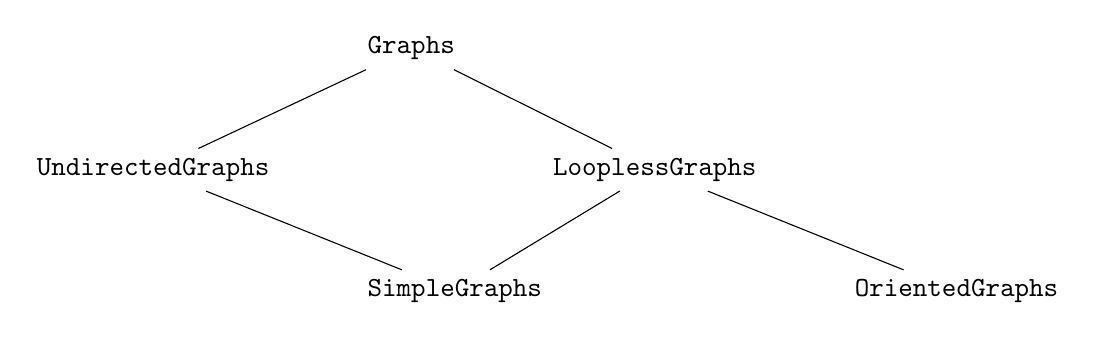
\begin{tikzpicture}[category/.style={font=\ttfamily}] \node (UG) [category]
{UndirectedGraphs}; \node (G) [category, above right=of UG] {Graphs}; \node
(SG) [category, below right=of UG] {SimpleGraphs}; \node (LG) [category, below
right=of G] {LooplessGraphs}; \node (OG) [category, below right=of LG]
{OrientedGraphs}; \draw (UG) -- (G) -- (LG) -- (OG); \draw (UG) -- (SG) --
(LG); \end{tikzpicture}   

This function is internally called by all graph constructing operations in \textsf{YAGS} to decide the graph category that the newly constructed graph is going to
belong. New graphs are always forced to comply with the \texttt{TargetGraphCategory}, so loops may be removed, and arrows may replaced by edges or vice versa,
depending on the category that the new graph belongs to. 

The \mbox{\texttt{\mdseries\slshape options stack}} is a mechanism provided by \textsf{GAP} to pass implicit parameters and is used by \texttt{TargetGraphCategory} so that the user may indicate the graph category she/he wants for the new
graph. 

 
\begin{Verbatim}[commandchars=!@|,fontsize=\small,frame=single,label=Example]
  !gapprompt@gap>| !gapinput@SetDefaultGraphCategory(SimpleGraphs);             |
  !gapprompt@gap>| !gapinput@g1:=CompleteGraph(2);                              |
  Graph( Category := SimpleGraphs, Order := 2, Size := 
  1, Adjacencies := [ [ 2 ], [ 1 ] ] )
  !gapprompt@gap>| !gapinput@g2:=CompleteGraph(2:GraphCategory:=OrientedGraphs);|
  Graph( Category := OrientedGraphs, Order := 2, Size := 
  1, Adjacencies := [ [ 2 ], [  ] ] )
  !gapprompt@gap>| !gapinput@DisjointUnion(g1,g2);|
  Graph( Category := LooplessGraphs, Order := 4, Size := 
  3, Adjacencies := [ [ 2 ], [ 1 ], [ 4 ], [  ] ] )
  !gapprompt@gap>| !gapinput@DisjointUnion(g1,g2:GraphCategory:=UndirectedGraphs);|
  Graph( Category := UndirectedGraphs, Order := 4, Size := 
  2, Adjacencies := [ [ 2 ], [ 1 ], [ 4 ], [ 3 ] ] )
\end{Verbatim}
 

In the previous examples, \texttt{TargetGraphCategory} was called internally exactly once for each new graph constructed with the
following parameters: 

 
\begin{Verbatim}[commandchars=!@|,fontsize=\small,frame=single,label=Example]
  !gapprompt@gap>| !gapinput@TargetGraphCategory();|
  <Category "SimpleGraphs">
  !gapprompt@gap>| !gapinput@TargetGraphCategory(:GraphCategory:=OrientedGraphs);|
  <Category "OrientedGraphs">
  !gapprompt@gap>| !gapinput@TargetGraphCategory([g1,g2]);                       |
  <Category "LooplessGraphs">
  !gapprompt@gap>| !gapinput@TargetGraphCategory([g1,g2]:GraphCategory:=UndirectedGraphs);|
  <Category "UndirectedGraphs">
\end{Verbatim}
 }

 

\subsection{\textcolor{Chapter }{Tetrahedron}}
\logpage{[ "B", 20, 2 ]}\nobreak
\hyperdef{L}{X7B44DDD485145773}{}
{\noindent\textcolor{FuncColor}{$\triangleright$\ \ \texttt{Tetrahedron\index{Tetrahedron@\texttt{Tetrahedron}}
\label{Tetrahedron}
}\hfill{\scriptsize (global variable)}}\\


 

The 1-skeleton of Plato's tetrahedron. 

 
\begin{Verbatim}[commandchars=!@|,fontsize=\small,frame=single,label=Example]
  !gapprompt@gap>| !gapinput@Tetrahedron;|
  Graph( Category := SimpleGraphs, Order := 4, Size := 
  6, Adjacencies := [ [ 2, 3, 4 ], [ 1, 3, 4 ], [ 1, 2, 4 ], 
    [ 1, 2, 3 ] ] )
\end{Verbatim}
 }

 

\subsection{\textcolor{Chapter }{TimeInSeconds}}
\logpage{[ "B", 20, 3 ]}\nobreak
\hyperdef{L}{X86C7A3E27AF64042}{}
{\noindent\textcolor{FuncColor}{$\triangleright$\ \ \texttt{TimeInSeconds({\mdseries\slshape })\index{TimeInSeconds@\texttt{TimeInSeconds}}
\label{TimeInSeconds}
}\hfill{\scriptsize (operation)}}\\


 

Returns the time in seconds since 1970-01-01 00:00:00 UTC as an integer. This
is useful to measure execution time. It can also be used to impose time
constraints on the execution of algorithms. Note however that the time
reported is the \emph{wall time}, not necessarily the time spent in the process you intend to measure. 


\begin{Verbatim}[commandchars=!@|,fontsize=\small,frame=single,label=Example]
  !gapprompt@gap>| !gapinput@TimeInSeconds();|
  1415551598
  !gapprompt@gap>| !gapinput@K:=CliqueGraph;;NumCli:=NumberOfCliques;;I:=Icosahedron;;|
  !gapprompt@gap>| !gapinput@t1:=TimeInSeconds();NumCli(K(K(K(K(I)))));TimeInSeconds()-t1;|
  1415551608
  44644
  103
\end{Verbatim}
 

Currently, this operation is not working on MS Windows. }

 

\subsection{\textcolor{Chapter }{TimesProduct}}
\logpage{[ "B", 20, 4 ]}\nobreak
\hyperdef{L}{X803A2BC67C63AA25}{}
{\noindent\textcolor{FuncColor}{$\triangleright$\ \ \texttt{TimesProduct({\mdseries\slshape G, H})\index{TimesProduct@\texttt{TimesProduct}}
\label{TimesProduct}
}\hfill{\scriptsize (operation)}}\\


 

Returns the times product\index{times product}\index{product of graphs!times}\index{product of graphs!tensor}, \mbox{\texttt{\mdseries\slshape G}}$\times$\mbox{\texttt{\mdseries\slshape H}}, of two graphs \mbox{\texttt{\mdseries\slshape G}} and \mbox{\texttt{\mdseries\slshape H}} (also known as the tensor product). 

The times product is computed as follows: 

For each pair of vertices $x \in \mbox{\texttt{\mdseries\slshape G}}, y \in \mbox{\texttt{\mdseries\slshape H}}$ we create a vertex $(x,y)$. Given two such vertices $(x,y)$ and $(x',y')$ they are adjacent iff $x \sim x'$ and $y \sim y'$. 


\begin{Verbatim}[commandchars=!@|,fontsize=\small,frame=single,label=Example]
  !gapprompt@gap>| !gapinput@g:=PathGraph(3);h:=CycleGraph(4);                              |
  Graph( Category := SimpleGraphs, Order := 3, Size := 
  2, Adjacencies := [ [ 2 ], [ 1, 3 ], [ 2 ] ] )
  Graph( Category := SimpleGraphs, Order := 4, Size := 
  4, Adjacencies := [ [ 2, 4 ], [ 1, 3 ], [ 2, 4 ], [ 1, 3 ] ] )
  !gapprompt@gap>| !gapinput@gh:=TimesProduct(g,h);         |
  Graph( Category := SimpleGraphs, Order := 12, Size := 
  16, Adjacencies := [ [ 6, 8 ], [ 5, 7 ], [ 6, 8 ], [ 5, 7 ], 
    [ 2, 4, 10, 12 ], [ 1, 3, 9, 11 ], [ 2, 4, 10, 12 ], 
    [ 1, 3, 9, 11 ], [ 6, 8 ], [ 5, 7 ], [ 6, 8 ], [ 5, 7 ] ] )
  !gapprompt@gap>| !gapinput@VertexNames(gh);                 |
  [ [ 1, 1 ], [ 1, 2 ], [ 1, 3 ], [ 1, 4 ], [ 2, 1 ], [ 2, 2 ], 
    [ 2, 3 ], [ 2, 4 ], [ 3, 1 ], [ 3, 2 ], [ 3, 3 ], [ 3, 4 ] ]
\end{Verbatim}
 }

 

\subsection{\textcolor{Chapter }{TorusGraph}}
\logpage{[ "B", 20, 5 ]}\nobreak
\hyperdef{L}{X87B9CA2A8552F40A}{}
{\noindent\textcolor{FuncColor}{$\triangleright$\ \ \texttt{TorusGraph({\mdseries\slshape n, m})\index{TorusGraph@\texttt{TorusGraph}}
\label{TorusGraph}
}\hfill{\scriptsize (function)}}\\


 

Returns (the underlying graph of) a triangulation of the torus on $n.m$ vertices. This graph is constructed using $\{1,2,\ldots, n\}\times\{1,2,\ldots, m\}$ as the vertex set; two of them being adjacent if their difference belongs to $\{(1,0),(0,1),(1,1)\}$ module ${\ensuremath{\mathbb Z}}_n\times{\ensuremath{\mathbb Z}}_m$. Hence, in the category of simple graphs, TorusGraph is a 6-regular graph
when $n,m\geq 3$. \index{graph!torus} 

 
\begin{Verbatim}[commandchars=!@|,fontsize=\small,frame=single,label=Example]
  TorusGraph(4,4);
  Graph( Category := SimpleGraphs, Order := 16, Size := 48, Adjacencies := 
  [ [ 2, 4, 5, 6, 13, 16 ], [ 1, 3, 6, 7, 13, 14 ], [ 2, 4, 7, 8, 14, 15 ], 
    [ 1, 3, 5, 8, 15, 16 ], [ 1, 4, 6, 8, 9, 10 ], [ 1, 2, 5, 7, 10, 11 ], 
    [ 2, 3, 6, 8, 11, 12 ], [ 3, 4, 5, 7, 9, 12 ], [ 5, 8, 10, 12, 13, 14 ], 
    [ 5, 6, 9, 11, 14, 15 ], [ 6, 7, 10, 12, 15, 16 ], [ 7, 8, 9, 11, 13, 16 ], 
    [ 1, 2, 9, 12, 14, 16 ], [ 2, 3, 9, 10, 13, 15 ], [ 3, 4, 10, 11, 14, 16 ], 
    [ 1, 4, 11, 12, 13, 15 ] ] )
\end{Verbatim}
 

When $n,m\geq 4$, \texttt{TorusGraph( \mbox{\texttt{\mdseries\slshape n}}, \mbox{\texttt{\mdseries\slshape m}} )} is actually a Whitney triangulation: Every triangle of the graph is a face of
the triangulation. The clique behavior of these graphs were extensively
studied in \cite{LN99}. However, this operation constructs the described graph for all $n,m \geq 1$. 

 
\begin{Verbatim}[commandchars=!@|,fontsize=\small,frame=single,label=Example]
  !gapprompt@gap>| !gapinput@TorusGraph(2,4);|
  Graph( Category := SimpleGraphs, Order := 8, Size := 
  20, Adjacencies := [ [ 2, 4, 5, 6, 8 ], [ 1, 3, 5, 6, 7 ], 
    [ 2, 4, 6, 7, 8 ], [ 1, 3, 5, 7, 8 ], [ 1, 2, 4, 6, 8 ], 
    [ 1, 2, 3, 5, 7 ], [ 2, 3, 4, 6, 8 ], [ 1, 3, 4, 5, 7 ] ] )
  !gapprompt@gap>| !gapinput@TorusGraph(2,3);|
  Graph( Category := SimpleGraphs, Order := 6, Size := 
  15, Adjacencies := [ [ 2, 3, 4, 5, 6 ], [ 1, 3, 4, 5, 6 ], 
    [ 1, 2, 4, 5, 6 ], [ 1, 2, 3, 5, 6 ], [ 1, 2, 3, 4, 6 ], 
    [ 1, 2, 3, 4, 5 ] ] )
\end{Verbatim}
 

Note that in these cases, \texttt{TorusGraph( \mbox{\texttt{\mdseries\slshape n}}, \mbox{\texttt{\mdseries\slshape m}} )} is not 6-regular nor a Whitney triangulation. }

 

\subsection{\textcolor{Chapter }{TreeGraph}}
\logpage{[ "B", 20, 6 ]}\nobreak
\hyperdef{L}{X7C7EAB207C957EB1}{}
{\noindent\textcolor{FuncColor}{$\triangleright$\ \ \texttt{TreeGraph({\mdseries\slshape arity, depth})\index{TreeGraph@\texttt{TreeGraph}}
\label{TreeGraph}
}\hfill{\scriptsize (operation)}}\\
\noindent\textcolor{FuncColor}{$\triangleright$\ \ \texttt{TreeGraph({\mdseries\slshape ArityList})\index{TreeGraph@\texttt{TreeGraph}}
\label{TreeGraph}
}\hfill{\scriptsize (operation)}}\\


 

Returns a tree, a connected cycle-free graph. In its second form, the vertices
at height \mbox{\texttt{\mdseries\slshape k}} (the root vertex has height 1 here) have \texttt{ArityList[\mbox{\texttt{\mdseries\slshape k}}]} children. In its first form, all vertices, but the leaves, have \mbox{\texttt{\mdseries\slshape arity}} children and the height of the leaves is \mbox{\texttt{\mdseries\slshape depth}}+1. \index{graph!tree} 

 
\begin{Verbatim}[commandchars=!@|,fontsize=\small,frame=single,label=Example]
  !gapprompt@gap>| !gapinput@TreeGraph(2,3);                                                  |
  Graph( Category := SimpleGraphs, Order := 15, Size := 
  14, Adjacencies := [ [ 2, 3 ], [ 1, 4, 5 ], [ 1, 6, 7 ], [ 2, 8, 9 ], 
    [ 2, 10, 11 ], [ 3, 12, 13 ], [ 3, 14, 15 ], [ 4 ], [ 4 ], [ 5 ], 
    [ 5 ], [ 6 ], [ 6 ], [ 7 ], [ 7 ] ] )
  !gapprompt@gap>| !gapinput@TreeGraph([3,2,2]);|
  Graph( Category := SimpleGraphs, Order := 22, Size := 
  21, Adjacencies := [ [ 2, 3, 4 ], [ 1, 5, 6 ], [ 1, 7, 8 ], 
    [ 1, 9, 10 ], [ 2, 11, 12 ], [ 2, 13, 14 ], [ 3, 15, 16 ], 
    [ 3, 17, 18 ], [ 4, 19, 20 ], [ 4, 21, 22 ], [ 5 ], [ 5 ], [ 6 ], 
    [ 6 ], [ 7 ], [ 7 ], [ 8 ], [ 8 ], [ 9 ], [ 9 ], [ 10 ], [ 10 ] ] )
\end{Verbatim}
 }

 

\subsection{\textcolor{Chapter }{TrivialGraph}}
\logpage{[ "B", 20, 7 ]}\nobreak
\hyperdef{L}{X82C1EADA7E3EE838}{}
{\noindent\textcolor{FuncColor}{$\triangleright$\ \ \texttt{TrivialGraph\index{TrivialGraph@\texttt{TrivialGraph}}
\label{TrivialGraph}
}\hfill{\scriptsize (global variable)}}\\


 

The one vertex graph. \index{graph!trivial} 

 
\begin{Verbatim}[commandchars=!@|,fontsize=\small,frame=single,label=Example]
  !gapprompt@gap>| !gapinput@TrivialGraph;|
  Graph( Category := SimpleGraphs, Order := 1, Size := 
  0, Adjacencies := [ [  ] ] )
\end{Verbatim}
 }

 }

 
\section{\textcolor{Chapter }{U}}\label{U}
\logpage{[ "B", 21, 0 ]}
\hyperdef{L}{X87EA348E87EA348E}{}
{
  

\subsection{\textcolor{Chapter }{UFFind}}
\logpage{[ "B", 21, 1 ]}\nobreak
\hyperdef{L}{X795BE08A79C126FC}{}
{\noindent\textcolor{FuncColor}{$\triangleright$\ \ \texttt{UFFind({\mdseries\slshape UFS, x})\index{UFFind@\texttt{UFFind}}
\label{UFFind}
}\hfill{\scriptsize (function)}}\\


 

For internal use. Implements the \mbox{\texttt{\mdseries\slshape find}} operation on the \mbox{\texttt{\mdseries\slshape union-find structure}}. }

 

\subsection{\textcolor{Chapter }{UFUnite}}
\logpage{[ "B", 21, 2 ]}\nobreak
\hyperdef{L}{X8105AD137ECF5AE4}{}
{\noindent\textcolor{FuncColor}{$\triangleright$\ \ \texttt{UFUnite({\mdseries\slshape UFS, x, y})\index{UFUnite@\texttt{UFUnite}}
\label{UFUnite}
}\hfill{\scriptsize (function)}}\\


 

For internal use. Implements the \mbox{\texttt{\mdseries\slshape unite}} operation on the \mbox{\texttt{\mdseries\slshape union-find structure}}. }

 

\subsection{\textcolor{Chapter }{UndirectedGraphs}}
\logpage{[ "B", 21, 3 ]}\nobreak
\hyperdef{L}{X7CC6D5C77C0CCFA3}{}
{\noindent\textcolor{FuncColor}{$\triangleright$\ \ \texttt{UndirectedGraphs({\mdseries\slshape G})\index{UndirectedGraphs@\texttt{UndirectedGraphs}}
\label{UndirectedGraphs}
}\hfill{\scriptsize (function)}}\\


 \texttt{UndirectedGraphs} is a graph category in \textsf{YAGS}. A graph in this category may contain edges and loops, but no arrows. The
parent of this category is \texttt{Graphs}. \index{graphs!undirected} 

 
\begin{Verbatim}[commandchars=!@|,fontsize=\small,frame=single,label=Example]
  !gapprompt@gap>| !gapinput@GraphByWalks([1,1],[1,2],[2,1],[3,2]:GraphCategory:=Graphs);|
  Graph( Category := Graphs, Order := 3, Size := 4, Adjacencies := 
  [ [ 1, 2 ], [ 1 ], [ 2 ] ] )
  !gapprompt@gap>| !gapinput@GraphByWalks([1,1],[1,2],[2,1],[3,2]:GraphCategory:=UndirectedGraphs);|
  Graph( Category := UndirectedGraphs, Order := 3, Size := 
  3, Adjacencies := [ [ 1, 2 ], [ 1, 3 ], [ 2 ] ] )
\end{Verbatim}
 }

 

\subsection{\textcolor{Chapter }{UnitsRingGraph}}
\logpage{[ "B", 21, 4 ]}\nobreak
\hyperdef{L}{X7FDA5DD47D181699}{}
{\noindent\textcolor{FuncColor}{$\triangleright$\ \ \texttt{UnitsRingGraph({\mdseries\slshape Rng})\index{UnitsRingGraph@\texttt{UnitsRingGraph}}
\label{UnitsRingGraph}
}\hfill{\scriptsize (operation)}}\\


 

Returns the graph G whose vertices are the elements of \mbox{\texttt{\mdseries\slshape Rng}} such that x is adjacent to y iff x+z=y for some unit z of \mbox{\texttt{\mdseries\slshape Rng}}. \index{graph!UnitsRing} 


\begin{Verbatim}[commandchars=!@|,fontsize=\small,frame=single,label=Example]
  !gapprompt@gap>| !gapinput@UnitsRingGraph(ZmodnZ(8));    |
  Graph( Category := SimpleGraphs, Order := 8, Size := 
  16, Adjacencies := [ [ 2, 4, 6, 8 ], [ 1, 3, 5, 7 ], [ 2, 4, 6, 8 ], 
    [ 1, 3, 5, 7 ], [ 2, 4, 6, 8 ], [ 1, 3, 5, 7 ], [ 2, 4, 6, 8 ], 
    [ 1, 3, 5, 7 ] ] )
\end{Verbatim}
 }

 }

 
\section{\textcolor{Chapter }{V}}\label{V}
\logpage{[ "B", 22, 0 ]}
\hyperdef{L}{X7E7AA1957E7AA195}{}
{
  

\subsection{\textcolor{Chapter }{VertexDegree}}
\logpage{[ "B", 22, 1 ]}\nobreak
\hyperdef{L}{X7B5898D98493A41D}{}
{\noindent\textcolor{FuncColor}{$\triangleright$\ \ \texttt{VertexDegree({\mdseries\slshape G, x})\index{VertexDegree@\texttt{VertexDegree}}
\label{VertexDegree}
}\hfill{\scriptsize (operation)}}\\


 

Returns the degree of vertex\index{degree!of a
vertex} \mbox{\texttt{\mdseries\slshape x}} in Graph \mbox{\texttt{\mdseries\slshape G}}. 

 
\begin{Verbatim}[commandchars=!@|,fontsize=\small,frame=single,label=Example]
  !gapprompt@gap>| !gapinput@g:=PathGraph(3);|
  Graph( Category := SimpleGraphs, Order := 3, Size := 
  2, Adjacencies := [ [ 2 ], [ 1, 3 ], [ 2 ] ] )
  !gapprompt@gap>| !gapinput@VertexDegree(g,1);|
  1
  !gapprompt@gap>| !gapinput@VertexDegree(g,2);|
  2
\end{Verbatim}
 }

 

\subsection{\textcolor{Chapter }{VertexDegrees}}
\logpage{[ "B", 22, 2 ]}\nobreak
\hyperdef{L}{X8406A82E7973EC00}{}
{\noindent\textcolor{FuncColor}{$\triangleright$\ \ \texttt{VertexDegrees({\mdseries\slshape G})\index{VertexDegrees@\texttt{VertexDegrees}}
\label{VertexDegrees}
}\hfill{\scriptsize (operation)}}\\


 

Returns the list of degrees of the vertices in graph \mbox{\texttt{\mdseries\slshape G}}. 

 
\begin{Verbatim}[commandchars=!@|,fontsize=\small,frame=single,label=Example]
  !gapprompt@gap>| !gapinput@g:=GemGraph;|
  Graph( Category := SimpleGraphs, Order := 5, Size := 
  7, Adjacencies := [ [ 2, 3, 4, 5 ], [ 1, 3 ], [ 1, 2, 4 ], 
    [ 1, 3, 5 ], [ 1, 4 ] ] )
  !gapprompt@gap>| !gapinput@VertexDegrees(g);|
  [ 4, 2, 3, 3, 2 ]
\end{Verbatim}
 }

 

\subsection{\textcolor{Chapter }{VertexNames}}
\logpage{[ "B", 22, 3 ]}\nobreak
\hyperdef{L}{X86050933823255F1}{}
{\noindent\textcolor{FuncColor}{$\triangleright$\ \ \texttt{VertexNames({\mdseries\slshape G})\index{VertexNames@\texttt{VertexNames}}
\label{VertexNames}
}\hfill{\scriptsize (attribute)}}\\


 

Return the list of names of the vertices of \mbox{\texttt{\mdseries\slshape G}}. The vertices of a graph in \textsf{YAGS} are always $\{1,2, \ldots, Order(G)\}$, but depending on how the graph was constructed, its vertices may have also
some \mbox{\texttt{\mdseries\slshape names}}, that help us identify the origin of the vertices. \textsf{YAGS} will always try to store meaningful names for the vertices. For example, in
the case of the LineGraph, the vertex names of the new graph are the edges of
the old graph. 

 
\begin{Verbatim}[commandchars=!@|,fontsize=\small,frame=single,label=Example]
  !gapprompt@gap>| !gapinput@g:=LineGraph(DiamondGraph);          |
  Graph( Category := SimpleGraphs, Order := 5, Size := 
  8, Adjacencies := [ [ 2, 3, 4 ], [ 1, 3, 4, 5 ], [ 1, 2, 5 ], 
    [ 1, 2, 5 ], [ 2, 3, 4 ] ] )
  !gapprompt@gap>| !gapinput@VertexNames(g);|
  [ [ 1, 2 ], [ 1, 3 ], [ 1, 4 ], [ 2, 3 ], [ 3, 4 ] ]
  !gapprompt@gap>| !gapinput@Edges(DiamondGraph);|
  [ [ 1, 2 ], [ 1, 3 ], [ 1, 4 ], [ 2, 3 ], [ 3, 4 ] ]
\end{Verbatim}
 }

 

\subsection{\textcolor{Chapter }{Vertices}}
\logpage{[ "B", 22, 4 ]}\nobreak
\hyperdef{L}{X79E4BB4F849AC8A1}{}
{\noindent\textcolor{FuncColor}{$\triangleright$\ \ \texttt{Vertices({\mdseries\slshape G})\index{Vertices@\texttt{Vertices}}
\label{Vertices}
}\hfill{\scriptsize (operation)}}\\


 

Returns the list [1..Order( \mbox{\texttt{\mdseries\slshape G}} )]. 

 
\begin{Verbatim}[commandchars=!@|,fontsize=\small,frame=single,label=Example]
  !gapprompt@gap>| !gapinput@Vertices(Icosahedron);|
  [ 1 .. 12 ]
\end{Verbatim}
 }

 }

 
\section{\textcolor{Chapter }{W}}\label{W}
\logpage{[ "B", 23, 0 ]}
\hyperdef{L}{X790AD29C790AD29C}{}
{
  

\subsection{\textcolor{Chapter }{WheelGraph}}
\logpage{[ "B", 23, 1 ]}\nobreak
\hyperdef{L}{X817EA60D828A765E}{}
{\noindent\textcolor{FuncColor}{$\triangleright$\ \ \texttt{WheelGraph({\mdseries\slshape n})\index{WheelGraph@\texttt{WheelGraph}}
\label{WheelGraph}
}\hfill{\scriptsize (operation)}}\\
\noindent\textcolor{FuncColor}{$\triangleright$\ \ \texttt{WheelGraph({\mdseries\slshape n, r})\index{WheelGraph@\texttt{WheelGraph}}
\label{WheelGraph}
}\hfill{\scriptsize (operation)}}\\


 

In its first form \texttt{WheelGraph} returns the wheel graph on \mbox{\texttt{\mdseries\slshape n}}+1 vertices. This is the cone of a cycle: a central vertex adjacent to all the
vertices of an \mbox{\texttt{\mdseries\slshape n}}-cycle. \index{graph!wheel} 

 
\begin{Verbatim}[commandchars=!@|,fontsize=\small,frame=single,label=Example]
  !gapprompt@gap>| !gapinput@WheelGraph(5);|
  Graph( Category := SimpleGraphs, Order := 6, Size := 
  10, Adjacencies := [ [ 2, 3, 4, 5, 6 ], [ 1, 3, 6 ], [ 1, 2, 4 ], 
    [ 1, 3, 5 ], [ 1, 4, 6 ], [ 1, 2, 5 ] ] )
\end{Verbatim}
 

In its second form, \texttt{WheelGraph} returns returns the wheel graph, but adding \mbox{\texttt{\mdseries\slshape r}}-1 layers, each layer is a new \mbox{\texttt{\mdseries\slshape n}}-cycle joined to the previous layer by a zigzagging 2\mbox{\texttt{\mdseries\slshape n}}-cycle. This graph is a triangulation of the disk. 

 
\begin{Verbatim}[commandchars=!@|,fontsize=\small,frame=single,label=Example]
  !gapprompt@gap>| !gapinput@WheelGraph(5,2);|
  Graph( Category := SimpleGraphs, Order := 11, Size := 
  25, Adjacencies := [ [ 2, 3, 4, 5, 6 ], [ 1, 3, 6, 7, 8 ], 
    [ 1, 2, 4, 8, 9 ], [ 1, 3, 5, 9, 10 ], [ 1, 4, 6, 10, 11 ], 
    [ 1, 2, 5, 7, 11 ], [ 2, 6, 8, 11 ], [ 2, 3, 7, 9 ], 
    [ 3, 4, 8, 10 ], [ 4, 5, 9, 11 ], [ 5, 6, 7, 10 ] ] )
  !gapprompt@gap>| !gapinput@WheelGraph(5,3);|
  Graph( Category := SimpleGraphs, Order := 16, Size := 
  40, Adjacencies := [ [ 2, 3, 4, 5, 6 ], [ 1, 3, 6, 7, 8 ], 
    [ 1, 2, 4, 8, 9 ], [ 1, 3, 5, 9, 10 ], [ 1, 4, 6, 10, 11 ], 
    [ 1, 2, 5, 7, 11 ], [ 2, 6, 8, 11, 12, 13 ], [ 2, 3, 7, 9, 13, 14 ],
    [ 3, 4, 8, 10, 14, 15 ], [ 4, 5, 9, 11, 15, 16 ], 
    [ 5, 6, 7, 10, 12, 16 ], [ 7, 11, 13, 16 ], [ 7, 8, 12, 14 ], 
    [ 8, 9, 13, 15 ], [ 9, 10, 14, 16 ], [ 10, 11, 12, 15 ] ] )
\end{Verbatim}
 }

 }

 
\section{\textcolor{Chapter }{Y}}\label{Y}
\logpage{[ "B", 24, 0 ]}
\hyperdef{L}{X8771504C8771504C}{}
{
  

\subsection{\textcolor{Chapter }{YAGSExec}}
\logpage{[ "B", 24, 1 ]}\nobreak
\hyperdef{L}{X8150D2E37EA1F25D}{}
{\noindent\textcolor{FuncColor}{$\triangleright$\ \ \texttt{YAGSExec({\mdseries\slshape ProgName, InString})\index{YAGSExec@\texttt{YAGSExec}}
\label{YAGSExec}
}\hfill{\scriptsize (operation)}}\\


 

For internal use. Calls external program \mbox{\texttt{\mdseries\slshape ProgName}} located in directory \texttt{YAGS-DIR/bin/} feeding it with \mbox{\texttt{\mdseries\slshape InString}} as input and returning the output of the external program as a string. \texttt{fail} is returned if the program could not be located. 


\begin{Verbatim}[commandchars=!@|,fontsize=\small,frame=single,label=Example]
  !gapprompt@gap>| !gapinput@YAGSExec("time","");|
  "1415551127\n"
  !gapprompt@gap>| !gapinput@YAGSExec("nauty","l=0$=1dacn=5 g1,2,3. xbzq");|
  "(4,5)\n(2,3)\n[2,3,4,5,1]\n[\"cb0c\",\"484f264\",\"b0e19f1\"]\n"
\end{Verbatim}
 

Currently, this operation is not working on MS Windows nor in Mac OS X. }

 

\subsection{\textcolor{Chapter }{YAGSInfo}}
\logpage{[ "B", 24, 2 ]}\nobreak
\hyperdef{L}{X865EB51A79C27268}{}
{\noindent\textcolor{FuncColor}{$\triangleright$\ \ \texttt{YAGSInfo\index{YAGSInfo@\texttt{YAGSInfo}}
\label{YAGSInfo}
}\hfill{\scriptsize (global variable)}}\\


 

A global record where much \textsf{YAGS}-related information is stored. This is intended for internal use, and much of
this information is undocumented, but some of the data stored here could
possibly be useful for advanced users. 

However, storing user information in this record and/or changing the values of
the stored information is discouraged and may produce unpredictable results
and an unstable system. 


\begin{Verbatim}[commandchars=!@|,fontsize=\small,frame=single,label=Example]
  !gapprompt@gap>| !gapinput@YAGSInfo;|
  rec( Arch := 1, DataDirectory := "/opt/gap4r8/pkg/yags/data", 
    Directory := "/opt/gap4r8/pkg/yags", 
    Draw := 
      rec( opts := [  ], 
        prog := "/opt/gap4r8/pkg/yags/bin/draw/application.linux64/draw" ), 
    InfoClass := YAGSInfoClass, InfoOutput := "*stdout*", Version := "0.0.1",
    graph6 := rec( BinListToNum := function( L ) ... end,
        BinListToNumList := function( L ) ... end,
        HararyList := [ [ 1, 0, 1 ], [ 2, 0, 1 ], [ 2, 1, 1 ],
            [ 3, 0, 1 ], [ 3, 1, 1 ], [ 3, 2, 1 ], [ 3, 3, 1 ],
            [ 4, 0, 1 ], [ 4, 1, 1 ], [ 4, 2, 1 ], [ 4, 3, 3 ],
            [ 4, 2, 2 ], [ 4, 3, 1 ], [ 4, 3, 2 ], [ 4, 4, 1 ],
  	  
     --- many more lines here ---
     
            [ 6, 13, 1 ], [ 6, 11, 7 ], [ 6, 11, 9 ], [ 6, 11, 8 ],
            [ 6, 12, 4 ], [ 6, 12, 5 ], [ 6, 13, 2 ], [ 6, 14, 1 ],
            [ 6, 15, 1 ] ], McKayN := function( n ) ... end,
        McKayR := function( L ) ... end,
        NumListToString := function( L ) ... end,
        NumToBinList := function( n ) ... end,
        PadLeftnSplitList6 := function( L ) ... end,
        PadRightnSplitList6 := function( L ) ... end,
        StringToBinList := function( Str ) ... end ) )
\end{Verbatim}
 }

 

\subsection{\textcolor{Chapter }{YAGSInfo.InfoClass}}
\logpage{[ "B", 24, 3 ]}\nobreak
\hyperdef{L}{X8602312E8239A2C0}{}
{\noindent\textcolor{FuncColor}{$\triangleright$\ \ \texttt{YAGSInfo.InfoClass\index{YAGSInfo.InfoClass@\texttt{YAGSInfo.InfoClass}}
\label{YAGSInfo.InfoClass}
}\hfill{\scriptsize (global variable)}}\\


 

\index{InfoClass@\texttt{InfoClass}}\index{progress reporting}\index{YAGSInfoClass@\texttt{YAGSInfoClass}} \index{InfoLevel@\texttt{InfoLevel}}\textsf{YAGS} uses the  \textbf{Reference: InfoLevel} mechanism in some algorithms for progress reporting. This is useful in
algorithms that may take a lot of time to finish, so the user is informed
about how much work is already done and how much work remains to be done; this
way, the user can decide whether to wait for the response or not. 

Enabling and disabling progress reporting is done by changing the \texttt{InfoLevel} of \texttt{YAGSInfo.InfoClass} to the appropiate level. The default \texttt{InfoLevel} for \texttt{YAGSInfo.InfoClass} is 0, and some of \textsf{YAGS} algorithms report at \texttt{InfoLevel} 1, and others at \texttt{InfoLevel} 3. 
\begin{Verbatim}[commandchars=!@|,fontsize=\small,frame=single,label=Example]
  !gapprompt@gap>| !gapinput@SetInfoLevel(YAGSInfo.InfoClass,3);           |
  !gapprompt@gap>| !gapinput@FullMonoMorphisms(PathGraph(3),CycleGraph(3));|
  #I [  ]
  #I [ 1 ]
  #I [ 1, 2 ]
  #I [ 1, 3 ]
  #I [ 2 ]
  #I [ 2, 1 ]
  #I [ 2, 3 ]
  #I [ 3 ]
  #I [ 3, 1 ]
  #I [ 3, 2 ]
  [  ]
  !gapprompt@gap>| !gapinput@SetInfoLevel(YAGSInfo.InfoClass,0);           |
  !gapprompt@gap>| !gapinput@FullMonoMorphisms(PathGraph(3),CycleGraph(3));|
  [  ]
\end{Verbatim}
 

The algorithms that report progress at \texttt{InfoLevel} 1 are \texttt{ParedGraph} (\ref{ParedGraph}) and \texttt{Cliques} (\ref{Cliques}), and also the algorithms that use those, namely: \texttt{CliqueGraph} (\ref{CliqueGraph}), \texttt{CliqueNumber} (\ref{CliqueNumber}), \texttt{CompletelyParedGraph} (\ref{CompletelyParedGraph}), \texttt{IsCliqueGated} (\ref{IsCliqueGated}) and \texttt{NumberOfCliques} (\ref{NumberOfCliques}). 

The algorithm that report at \texttt{InfoLevel} 3 is \texttt{Backtrack} (\ref{Backtrack}) and the algorithms that use that one, namely: \texttt{BacktrackBag} (\ref{BacktrackBag}), \texttt{CompletesOfGivenOrder} (\ref{CompletesOfGivenOrder}), \texttt{Orientations} (\ref{Orientations}) and all the morphism-related operations in Chaper \ref{morphismsofgraphs}. The meaning of the progress strings reported in all these functions are
described in Section \ref{debuggingbacktracks}. 

The output of the progress info may be redirected to a file or character
device by setting the variable \texttt{YAGSInfo.InfoOutput} (\ref{YAGSInfo.InfoOutput}) accordingly. }

 

\subsection{\textcolor{Chapter }{YAGSInfo.InfoOutput}}
\logpage{[ "B", 24, 4 ]}\nobreak
\hyperdef{L}{X837885A8851D670D}{}
{\noindent\textcolor{FuncColor}{$\triangleright$\ \ \texttt{YAGSInfo.InfoOutput\index{YAGSInfo.InfoOutput@\texttt{YAGSInfo.InfoOutput}}
\label{YAGSInfo.InfoOutput}
}\hfill{\scriptsize (global variable)}}\\


 

The output of the progress info reported by some algorithms (see \texttt{YAGSInfo.InfoClass} (\ref{YAGSInfo.InfoClass})) may be redirected to a file by setting the variable \texttt{YAGSInfo.InfoOutput} accordingly. The default value \texttt{YAGSInfo.InfoOutput:="*stdout*"} means the console; but setting the name of a file as the value of \texttt{YAGSInfo.InfoOutput} sends the output to that file. In Unix-like systems, we can also use the name
of a character device (like \texttt{"/dev/null"}, \texttt{"/dev/tty"} or \texttt{"/dev/pts/1"}) to redirect the progress info output to that device. }

 }

 }

\def\bibname{References\logpage{[ "Bib", 0, 0 ]}
\hyperdef{L}{X7A6F98FD85F02BFE}{}
}

\bibliographystyle{mapbib}
\bibliography{biblio}

\addcontentsline{toc}{chapter}{References}

\def\indexname{Index\logpage{[ "Ind", 0, 0 ]}
\hyperdef{L}{X83A0356F839C696F}{}
}

\cleardoublepage
\phantomsection
\addcontentsline{toc}{chapter}{Index}


\printindex

\newpage
\immediate\write\pagenrlog{["End"], \arabic{page}];}
\immediate\closeout\pagenrlog
\end{document}
